
\documentclass[twoside,a4,12p,oepnright]{report} %,draft,openright]
\makeatletter
	\setlength{\@fptop}{0pt}
\makeatother
%\documentclass[twoside,11pt,openright]
%% Latex documents that need direct input
%  The following command loads a graphics package to include images
%  in the document. It may be necessary to specify a DVI driver option,
%  e.g., [dvips], but that may be inappropriate for some LaTeX
%  installations.
\usepackage[]{graphicx}

% In order to include files without having a clear page using \include*,
% the newclude package is required
%\usepackage{newclude}

% Required for acronyms
% use \acresetall to reset the acroyms counter
% macros=True, allows for calling \myTriger rather than \ac{myTriger}
\usepackage[single=true, macros=false, xspace=true]{acro}

% In SPIE template, biblatex can NOT be used to manage the referencing
%
%\usepackage[style=spiebib, backend=biber]{biblatex}

% Clever cross referencing. Using cleverref, instead of writting
% figure~\ref{...} or equation~\ref{...}, only \cref{...} is required.
% The package interprates the references and introduces the figure, fig.,
% equation, eq., etc keywords. \Cref forces first letter capital.
% >> WARNING: This package needs to be loaded after hyperref, math packages,
%             etc. if used.

%             Cleveref is recomended to load late
\usepackage{amsmath}
\usepackage{hyperref}
\usepackage{cleveref}
% To create random text use lipsum
\usepackage{lipsum}
\usepackage{siunitx}
\usepackage[doublespacing]{setspace}
\usepackage{scalefnt,lmodern}
\DeclareSIUnit\px{px}
\usepackage{epsf,graphicx,subfig}
\usepackage{epsfig}
\usepackage{epstopdf}
\usepackage{latexsym,amssymb}
\usepackage{lipsum}
\usepackage{xcolor}
\usepackage{algorithm}
\usepackage{algorithmic}
\usepackage{tabularx}
\usepackage{longtable}
\usepackage{afterpage}
\usepackage{booktabs}
\usepackage{courier}
\usepackage{array,multirow}
\usepackage{pbox}
\usepackage{colortbl,bigdelim}
\usepackage{arydshln}
\usepackage{enumerate}
\usepackage{threeparttable}
\usepackage{lscape}
\usepackage{pdflscape}
\usepackage{emptypage}
%\usepackage{xepersian}
%\usepackage{bidi}% this should be the last package to load.

%\usepackage{wrapfig} 
%\usepackage{setspace,cite}
%\usepackage{moreverb} % Verbatim-Umgebung
%\usepackage{cite}	  %Zitate
%\usepackage{xcolor}		%colors
%\usepackage{pxfonts}
\usepackage{tikz,xifthen}
\usetikzlibrary{shadows,arrows,calc,positioning,backgrounds,snakes,decorations.text,decorations.markings,shapes,patterns,fit,chains,decorations.pathreplacing}
\usepackage{url}
\hypersetup{
   colorlinks,%
   citecolor=black,%
   %figurecolor = green,%
   filecolor=black,%
   linkcolor=black,%
   urlcolor=black
}

% for margins left, right top bottom
\usepackage{anysize}
\marginsize{4cm}{2.5cm}{4cm}{4cm}

%\usepackage{draft} %draft option - doesn't put full figures in - useful when editing
%does the headers on the pages - keep in
\usepackage{fancyhdr}

%\urldef{\mailsa}\path|{alfred.hofmann, ursula.barth, ingrid.haas, frank.holzwarth,|
%\urldef{\mailsb}\path|anna.kramer, leonie.kunz, christine.reiss, nicole.sator,|
%\urldef{\mailsc}\path|erika.siebert-cole, peter.strasser, lncs}@springer.com|    

\DeclareMathOperator*{\argmin}{arg\,min}
\DeclareMathOperator*{\argmax}{arg\,max}
\definecolor{dgreen}{rgb}{ 0    0.52    0.25}
%\newcommand{\fullyGuidedColor}{(dark-green)}

\let\origdoublepage\cleardoublepage
\newcommand{\clearemptydoublepage}{%
  \clearpage
  {\pagestyle{empty}\origdoublepage}%
}

%\usepackage[T1]{fontenc}
%\usepackage[utf8]{inputenc}
\usepackage[catalan, english]{babel}
%\usepackage{lmodern}

%%Definició de la ela geminada per tal que accepti el punt volat del teclat
%\def·#1{%
%  \ifmmode
%    \cdot #1
%    %\csname normal@char\string"\endcsname l%
%  \else%
%    \def\argument{#1}%
%    \if\argument l%
%      \leftllkern=0pt\rightllkern=0pt\raiselldim=0pt%
%      \setbox0\hbox{l}\setbox1\hbox{l\/}\setbox2\hbox{.}%
%      \advance\raiselldim by \the\fontdimen5\the\font
%      \advance\raiselldim by -\ht2%
%      \leftllkern=-.25\wd0%
%      \advance\leftllkern by \wd1%
%      \advance\leftllkern by -\wd0%
%      \rightllkern=-.25\wd0%
%      \advance\rightllkern by -\wd1%
%      \advance\rightllkern by \wd0%
%      \allowhyphens\discretionary{-}{l}%
%      {\hbox{}\kern\leftllkern\raise\raiselldim\hbox{.}%
%        \kern\rightllkern\hbox{l}}\allowhyphens%
%    \else
%      \if\argument L%
%        \leftllkern=0pt\rightllkern=0pt\raiselldim=0pt%
%        \setbox0\hbox{L}\setbox1\hbox{L\/}\setbox2\hbox{.}%
%        \advance\raiselldim by .5\ht0%
%        \advance\raiselldim by -.5\ht2%
%        \leftllkern=-.125\wd0%
%        \advance\leftllkern by \wd1%
%        \advance\leftllkern by -\wd0%
%        \rightllkern=-\wd0%
%        \divide\rightllkern by 6%
%        \advance\rightllkern by -\wd1%
%        \advance\rightllkern by \wd0%
%        \allowhyphens\discretionary{-}{L}%
%        {\hbox{}\kern\leftllkern\raise\raiselldim\hbox{.}%
%           \kern\rightllkern\hbox{L}}\allowhyphens%
%      \else
%        #1
%      \fi
%    \fi
%  \fi
%  }
        % contains the latex packages
%%%%%%%%%%%%%%%%%%%%%%%%%%%%%%%%%%%%%%%%%%%%%%%%%%%%%%%%%%%%% 
%>>>> uncomment following for page numbers
% \pagestyle{plain}    
%>>>> uncomment following to start page numbering at 301 
%\setcounter{page}{301} 
      % contains package and variables init.
%% Acronym definition example using glossaries package
%% \usepackage{acro} is required
%% 
%% For a powerful usage of the acro package look at http://tex.stackexchange.com/questions/135975/how-to-define-an-acronym-by-using-other-acronym-and-print-the-abbreviations-toge

\DeclareAcronym{cad}{
  short = CAD, 
  long = Computer-Aided Diagnosis
}
\DeclareAcronym{us1}{
	short = US, 
	long = ultra-sound
}
\DeclareAcronym{cds}{
  short = CDS, 
  long = Clinical Diagnosis Support 
}
\DeclareAcronym{npd}{
  short = NPD, 
  long = nonpolarized dermoscope
}
\DeclareAcronym{clsm}{
  short = CLSM, 
  long = confocal laser scanning microscopy
}
\DeclareAcronym{pd}{
  short = PD, 
  long = polarized dermoscope
}
\DeclareAcronym{oct}{
  short = OCT, 
  long = optical coherence tomography 
}
\DeclareAcronym{psls}{
  short = PSLs, 
  long = pigmented skin lesions
}
\DeclareAcronym{psl}{
  short = PSL, 
  long = pigmented skin lesion
}
\DeclareAcronym{who}{
  short = WHO, 
  long = World Health Organization
}
\DeclareAcronym{ct}{
  short = CT, 
  long = computed tomography
}
\DeclareAcronym{mri}{
  short = MRI, 
  long = Magnetic Resonance Imaging
}
\DeclareAcronym{acs}{
  short = ACS, 
  long = American Cancer Society
}
\DeclareAcronym{msi}{
  short = MSI,
  long =  multispectral imaging
}
\DeclareAcronym{msd}{
  short = MSD,
  long =  multispectral dermoscope
}
\DeclareAcronym{pi}{
  short = PI, 
  long = polarized imaging 
}
\DeclareAcronym{nir}{
  short = NIR, 
  long = near infrared 
}
\DeclareAcronym{uv}{
  short = UV, 
  long = ultra-violet 
}
% classifiers 
\DeclareAcronym{rf}{
  short = RF,
  long = Random Forests
}
\DeclareAcronym{svm}{
  short = SVM,
  long = support Vector Machine
}
\DeclareAcronym{nb}{
  short = NB,
  long = Naive Bayes
}
\DeclareAcronym{gb}{
  short = GB,
  long = Gradient Boosting
}
\DeclareAcronym{ecoc}{
  short = ECOC,
  long = Error Correcting Output Coding
}
\DeclareAcronym{adb}{
	short = AdB, 
	long = AdaBoost
}
\DeclareAcronym{svd}{
  short = SVD,
  long =  Singular Value Decomposition 
}
\DeclareAcronym{omp}{
	short = OMP, 
	long = orthogonal matching pursuit
}
\DeclareAcronym{bp}{
	short = BP, 
	long = basis pursuit
}
\DeclareAcronym{map}{
	short = MAP, 
	long = Maximum a Posteriori
}
\DeclareAcronym{ml}{
	short = ML, 
	long = Maximum Likelihood
}
\DeclareAcronym{mlp}{
	short = MLP, 
	long = Multi Layer Perceptron
}
\DeclareAcronym{dt}{
	short = DT,
	long = Decision Trees
}
\DeclareAcronym{qda}{
	short= QDA, 
	long = Quadratic Discriminant Analysis
}
\DeclareAcronym{lmt}{
	short = LMT,
	long = Logistic Model Trees
}
%segmentation and pre-processing
\DeclareAcronym{gvf}{
	short = GVF, 
	long = Gradient Vector Flow  
}
\DeclareAcronym{jpeg}{
	short = JPEG, 
	long = Joint Photographic Experts Group
}
\DeclareAcronym{pde}{
	short = PDE, 
	long = partial differential equations
}
\DeclareAcronym{awb}{
	short = AWB, 
	long = auto-white-balance
}
\DeclareAcronym{cwb}{
	short = CWB, 
	long = custom-white-balance
}
%features
\DeclareAcronym{hog}{
	short = HOG, 
	long = Histogram of Oriented Gradients
}
\DeclareAcronym{lbp}{
	short = LBP, 
	long = Local Binary Pattern
}
\DeclareAcronym{glcm}{
	short = GLCM, 
	long = Grey-Level Co-Occurrence Matrix 
}
\DeclareAcronym{sift}{
	short = SIFT, 
	long = Scale-Invariant Feature Transform
}
\DeclareAcronym{surf}{
	short = SURF, 
	long = Speeded Up Robust Features
}
\DeclareAcronym{clbp}{
	short = CLBP,
	long = Completed Local Binary Pattern
}

%dimension reductions
\DeclareAcronym{mrmr}{
	short = mRMR, 
	long = Minimum Redundancy Maximum Relevance
}
\DeclareAcronym{cfs}{
	short = CFS, 
	long = Correlation Feature Selection
}
\DeclareAcronym{sffs}{
	short = SFFS, 
	long = Sequential Forward Feature Selection
}
\DeclareAcronym{sbfs}{
	short = SBFS, 
	long = Sequential Backward Feature Selection
}
\DeclareAcronym{pca}{
  short = PCA, 
  long = Principal Component Analysis 
}
\DeclareAcronym{lda}{
	short = LDA, 
	long = Linear Discriminant Analysis
}
\DeclareAcronym{lle}{
	short = LLE, 
	long = Locally Linear Embedding
}
\DeclareAcronym{mvu}{
	short = MVU, 
	long = Maximum Variance Unfolding
}
\DeclareAcronym{bow}{
	short = BoW, 
	long = Bag of Words
}
\DeclareAcronym{scf}{
	short = SCF, 
	long = Sparse Coded Features 
}
% balancing
\DeclareAcronym{os}{
	short = OS,
	long = Over-Sampling
}
\DeclareAcronym{us}{
	short = US, 
	long = Under-Sampling
}
\DeclareAcronym{smote}{
	short = SMOTE, 
	long = Synthetic Minority Over-Sampling
}
\DeclareAcronym{tl}{
	short= TL, 
	long = Tomek-Link
}
\DeclareAcronym{nm}{
	short = NM,
	long = NearMiss
}	
\DeclareAcronym{nm1}{
	short = NM1, 
	long = NearMiss-1
}
\DeclareAcronym{nm2}{
	short = NM2, 
	long = NearMiss-2
}
\DeclareAcronym{nm3}{
	short = NM3, 
	long = NearMiss-3
}
\DeclareAcronym{cus}{
	short = CUS, 
	long = Clustering
}
\DeclareAcronym{ncr}{
	short = NCR, 
	long = Neighborhood Cleaning Rule
}
\DeclareAcronym{ros}{
	short = ROS, 
	long = Random Over-Sampling
}
\DeclareAcronym{rus}{
	short = RUS, 
	long = Random Under-Sampling
}
\DeclareAcronym{nn}{
	short = NN, 
	long = Nearest Neighbor
}
\DeclareAcronym{enn}{
	short = ENN, 
	long = Editted Nearest Neighbor
}
\DeclareAcronym{mp}{
	short = MP, 
	long = matching pursuit
}
\DeclareAcronym{dos}{
	short = DOS, 
	long = data space over-sampling
}
% validation and Evaluation
\DeclareAcronym{loocv}{
	short = LOOCV,
	long = leave-one-out-cross-validation
}
\DeclareAcronym{kcv}{
	short = k-CV, 
	long = k fold cross-validation
}
\DeclareAcronym{tp}{
	short = TP, 
	long = true positive
}
\DeclareAcronym{tn}{
	short = TN, 
	long = true negative
}
\DeclareAcronym{fp}{
	short = FP, 
	long = false positive
}
\DeclareAcronym{fn}{
	short = FN, 
	long = false negative
}
\DeclareAcronym{se}{
  	short = SE,
  	long = sensitivity
}
\DeclareAcronym{sp}{
  	short = SP,
  	long =  specificity
}
\DeclareAcronym{ppv}{
	short = PPV, 
	long = precision (positive predictive value)
}
\DeclareAcronym{acc}{
	short = ACC, 
	long = accuracy
}
\DeclareAcronym{roc}{
	short = ROC,
	long = Recever Operating Characteristics
}
\DeclareAcronym{fpr}{
	short = FPR,
	long = false positive rate
}
\DeclareAcronym{auc}{
	short = AUC,
	long = area under the curve
}
\DeclareAcronym{ann}{
	short = ANN,
	long = Artificial Neural Network
}
\DeclareAcronym{delm}{
	short = D-ELM,
	long= digital epiluminescene microscopy images
}
% The methdo Chapter3 
\DeclareAcronym{pdf}{
	short = pdf,
	long = probablity density function
}
\DeclareAcronym{fcm}{
	short = FCM, 
	long = Fuzzy-C-\textit{means}
}
\DeclareAcronym{staple}{
	short = STAPLE,
	long = simultaneous truth and performance level estimation
}
\DeclareAcronym{dog}{
	short = DoG, 
	long = difference of gaussian
}
\DeclareAcronym{bd}{
  short = BD,
  long = barrel deformation
}

\DeclareAcronym{rdgm}{
  short = RDGM,
  long = random deformation using gaussian motion 
}
% Polarimetry 
\DeclareAcronym{dop}{
	short = DOP, 
	long = degree of polarization
}
\DeclareAcronym{dolp}{
	short = DOLP, 
	long = degree of linear polarization
}
\DeclareAcronym{docp}{
	short = DOCP, 
	long = degree of circular polarization
}
\DeclareAcronym{lctf}{
	short = LCTF, 
	long = liquid crystal filter
}
\DeclareAcronym{pem}{
	short = PEM,
	long = photoelastic modulator 
}
\DeclareAcronym{ac}{
	short = AC,
	long = Alternative Current
}
\DeclareAcronym{dc}{
	short = DC, 
	long = Direct Current
}
\DeclareAcronym{psg}{
	short = PSG,
	long = polarized state generator
}
\DeclareAcronym{psa}{
	short = PSA, 
	long = polarized state analyzer
}
\DeclareAcronym{lc}{
	short = LC,
	long = liquid crystal variable retarders
}
\DeclareAcronym{cmos}{
	short = CMOS, 
	long = complementary metal oxide semiconductor
}
\DeclareAcronym{ufraw}{
	short = UFRaw,
	long =  Unidentified Flying Raw
}
\DeclareAcronym{tiff}{
	short = TIFF, 
	long= Tagged Image File Format
}
\DeclareAcronym{aolp}{
	short = AOLP, 
	long = angle of linear polarization
}
\DeclareAcronym{dofp}{
	short = DoFP, 
	long  = division-of-focal-plane
}

      % contains the acronims


%omitting any of these makes the thesis compile without the omitted
%chapter - good for editing single chapters.
%\includeonly{header,introduction,problem,stateart,methodology,results,conclusion,appendix}

\begin{document}
\newpage

%Puts page numbering of preamble in roman and of main body of thesis in
%arabic. Also defines how chapters and sections are made
%\pagenumbering{arabic}
%\setcounter{page}{1} \pagestyle{fancy}
%\renewcommand{\chaptermark}[1]{\markboth{\chaptername}}
%%\ \thechapter:\,\ #1}{}}
%\renewcommand{\sectionmark}[1]{\markright{\thesection\,\ #1}}

%DEFINES TITLE PAGE, and contains abstract, acknowledgements, etc.
%sets up headers for lefthand and righthand pages. To alter, edit
%these lines and the chaptermark/sectionmark lines above
\addtolength{\headheight}{3pt} \fancyhead{}
\fancyhead[LE]{\sl\leftmark} \fancyhead[LO,RE]{\rm\thepage}
\fancyhead[RO]{\sl\rightmark} \fancyfoot[C,L,E]{}

%%%%%%%%%%%%%%%%%%%%%%%%%%%%%%%%%%%%%%%%%%%%%%%%%%%%%%%%%%%%%%%%%%%%%%%%%%%
% This is a sample header for a sample dissertation. Fill in the name,
% and the other information. LaTeX will work out the table of
% content, the list of figures and of tables for you.
%%%%%%%%%%%%%%%%%%%%%%%%%%%%%%%%%%%%%%%%%%%%%%%%%%%%%%%%%%%%%%%%%%%%%%%%%%%
\pagenumbering{gobble} 

\newpage
\thispagestyle{empty}

% ******* Title page  One *******
% *******************************
\vspace{3cm}
\begin{center}

\includegraphics[width=0.5\textwidth]{Figures/logo/udglogo2.png}\

\includegraphics[width= 0.4\textwidth]{Figures/logo/logoub.png}
\end{center}
\vspace{0.5cm}
\begin{center}
PhD Thesis
\end{center}
\vspace{1cm}
\begin{center}
\LARGE{\LARGE{\textbf{An approach to melanoma classification exploiting polarization information
%Classification of melanoma lesions using cross-polarized and Stokes polarimetry
}}}
\end{center}
\vspace{1.5cm}
\begin{center}
{\large{\textbf{Mojdeh Rastgoo}}}
\end{center}
\vspace{1.5cm}
\begin{center}
\textbf{2016}
\end{center}

%\clearpage 
%\newpage
%\thispagestyle{empty}
\cleardoublepage

\newpage
\thispagestyle{empty}

% ******* Title page Two *******
% ******************************
\vspace{3cm}
\begin{center}

\includegraphics[width=0.5\textwidth]{Figures/logo/udglogo2.png}\

\includegraphics[width= 0.4\textwidth]{Figures/logo/logoub.png}
\end{center}
\vspace{0.3cm}
\begin{center}
PhD Thesis
\end{center}
\vspace{0.7cm}
\begin{center}
\LARGE{\LARGE{\textbf{An approach to melanoma classification exploiting polarization information
%Classification of melanoma lesions using non-conventional screening techniques
}}}
\end{center}
\vspace{0.5cm}
\begin{center}
{\large{\textbf{Mojdeh Rastgoo}}}
\end{center}
\vspace{0.5cm}
\begin{center}
\textbf{2016}
\end{center}
\vspace{0.5cm}
\begin{center}
DOCTORAL PROGRAM IN TECHNOLOGY 
\end{center}
\vspace{0.5cm}
\begin{center}
Supervised by: Dr.~Rafael~Garc\'{\i}a, Dr.~Franck~Marzani, and Dr.~Olivier~Morel
\end{center}
\vspace{0.5cm}
\begin{center}
Work submitted to the universitat de Girona and Universit\'e de Bourgogne in partial fulfillment of the requirements for the degree of Doctor of Philosophy
\end{center}

\cleardoublepage


%******** Dedication Page ********
%*********************************

\newpage
\thispagestyle{empty}

\begin{flushright}
\begin{tabular}{l}
\textit{Dedicated to Mojgan, Majid, Vahid, Moujan, and Guillaume}
\end{tabular}
\end{flushright}

\cleardoublepage

%************************************
\pagenumbering{roman}
\setcounter{page}{5} \pagestyle{plain}

\newpage
\thispagestyle{empty}
% Publication 
\chapter*{Publications}
%\addcontentsline{toc}{chapter}{\protect\numberline{Publication\hspace{-96pt}}}
\textbf{Journal:}\\
\noindent \textbf{M. Rastgoo, O. Morel, F. Marzani and R. Garcia}, ``Automatic Differentiation of Melanoma from Dysplastic Nevi'', \emph{Computerized Medical Imaging and Graphics}, vol.43, pp 44-52, 2015\\\\

\noindent \textbf{International Conferences:}\\
\noindent\textbf{M. Rastgoo, G. Lemaitre, J. Massich, O.Morel, F. Marzani, R. Garcia and F. Meriaudeau}, ``Tackling the Problem of Data Imbalancing for Melanoma Classification'', \emph{$3^{rd}$ International Conference on BIOIMAGING 2016.} Rome: Italy (February 2016)\\

\noindent\textbf{M. Rastgoo, G. Lemaitre, O.Morel, J. Massich, F. Marzani, R. Garcia and D. Sidibe}, ``Classification of melanoma lesions using sparse coded features and radnom forests'', \emph{SPIE Medical Imaging 2016.} San Diego: USA (February 2016)\\

\noindent\textbf{M. Rastgoo, O. Morel, F. Marzani and R. Garcia}, ``Ensemble Approach for Differentiation of Malignant Melanoma'', \emph{International Conference on Quality Control and Artificial Vision (QCAV) 2015.} Le Creusot: France (June 2015)\\

\cleardoublepage

%**********************************
\addcontentsline{toc}{chapter}{List of Abbreviations}
\printacronyms[name = Abbreviations]

\addcontentsline{toc}{chapter}{\listfigurename}
\listoffigures
\cleardoublepage
%\listoffigures
\addcontentsline{toc}{chapter}{\listtablename}
\listoftables
\cleardoublepage

%************************************

\newpage
\thispagestyle{empty}
\chapter*{Acknowledgments}	
\singlespacing
I am absolutely grateful to my supervisors, Rafael Garc\'ia, Franck Marzani and Olivier Morel.	
Without their supports, guidelines, insights and encouragements, this work would not be simply possible. 

I would also like to thank Fabrice M\'eriaudeau for his constant support.
Thanks to D\'esir\'e Sidib\'e as well for sharing his brilliant ideas. 
Thanks to Pablo Iglesias and Beatriz Alejo Galindo for being patient and providing me with the medical insight and data; also to Dr. Josep Malvehy and Susana Puig for sharing their time and valuable clinical insights for the improvement of this project.
A particular thanks to Steven Jacques for sharing his valuable knowledge and most importantly being inspiring.

I would like to thank my friends; Habib, Sarah, Amanda, Sonia, Sharad, Shihav, David, Abir, Mohamed, Cansen, Qinglin, Richa, Armine, Priyanka, Joan -for having his unique way of thinking- and Konstantin whom patiently and perfectly corrected the final manuscript and provided me with his thoughtful ideas. 
Thank you all for the shared happy moments and your help and support during this time.

Also I would like to thank my colleagues, Nuno, Tudor, L\'aszl\'o, Josep, Ricard P., Ricard C. and Konstantin for all the interesting lab meetings and their help for the final preparation of the thesis; to Joseta, Mireia and Montse, for being always there and helping me with endless amount of paperwork and questions.

My gratitude, as well, to the anonymous reviewers and the members of the defense panel for evaluating my work.
I would also like to acknowledge AGAUR FI-DGR 2012 grant, provided by the Autonomous Government of Catalunia which is the sole reason for existence of this thesis.
It is an honored to be among its holders. 

Foremost, I would like to thank my family that has always being there for me, despite the long distance between us.
Their love, support and motivation gave me the strength to finish the thesis.
My most loving thanks to my parents, Mojgan and Majid, brother Vahid, sister Moujan, both grandmothers: Maman Alam and Maman joon, aunt Mahboubeh, aunt Manijeh, cousin Sudeh, cousin Somayeh and cousin Maryam.
And all the family.

I would like to thank Ginette, Patrice, Cedric, Vero, Julian and Sarah for being my family here.


Last but not least, I want to thank my husband and best colleague Guillaume for his love and support and being my best friend. 
  

 

%\addcontentsline{toc}{chapter}{\protect\numberline{Acknowledgments\hspace{-96pt}}}
\cleardoublepage
\doublespacing

%************************************

\tableofcontents
\cleardoublepage

%\vspace{1.2cm}
%\begin{center}
%
%\vspace{0.9cm}
%{\large A Thesis Submitted for the Degree of Doctor of Philosophy in computer vision and robotics (Universitat de Girona) and Le2i laboratory (Univerist\'e de Bourgogne)\\\vspace{0.3cm} $\cdot$ 2015
%$\cdot$}
%\end{center}
%\singlespacing

\singlespacing
%ABSTRACT
%\begin{abstract}
\begin{center}\textbf{Abstract}\\\end{center}
Malignant melanoma is the deadliest of skin cancers and causes the majority of deaths in comparison to other skin-related malignancies.
Yet it is the most treatable type of cancer, thanks to its early diagnosis.
Subsequently, early diagnosis is crucial for patient survival rate and numerous \ac{cad} systems have been proposed by the research community to assist dermatologists in early diagnosis.
These systems are based on the most common skin imaging modality, cross-polarized dermoscopy.
Cross-polarized dermoscopes (PD) allow for the visualization of the subsurface anatomic structure of the epidermis and papillary dermis and eliminate the specular reflection of the surface.
Although this modality has been used extensively, the full potential of polarized measurements has not been realized in the field of skin imaging.

This research first extensively analyzes different aspects of the automated classification of \ac{psls} and proposes a \ac{cad} system for automatic recognition of melanoma lesions based on the PD images.
The proposed \ac{cad} system is evaluated over extensive experiments on two dermoscopic datasets.
Later for further investigation of polarized imaging, a novel partial Stokes polarimeter system is proposed.
This system is able to acquire polarized images of in-vivo \ac{psls} and capture the epidermis and superficial dermal layers, where skin lesions are often originated.
The polarized and dermoscopy properties of the acquired images are then analyzed to propose a new \ac{cad} system based on image polarimetry.
The initial tests with the first prototype of Stokes polarimeter revealed the potential and benefits of such systems for providing additional information beyond RGB images acquired with PD devices.
In order to acquire a wider clinical dataset and identify the drawbacks of the first prototype, this device is currently being used in the Melanoma Unit at the Clinic Hospital of Barcelona.
\clearpage

%\end{abstract}

%%% Catalan Abstract %%%%%%%%%%%%%%%%%%%%%%%%%%%%%%%%%%%%%%%%%%%%%%%%%%%%%% 
\begin{center}\textbf{Resum}\\\end{center}
El melanoma maligne \'es el m\'es mortal dels c\`ancers de pell i provoca la majoria de les morts en comparaci\'o amb altres tumors malignes relacionats amb la pell.
No obstant aix\`o, \'es el tipus m\'es tractable de c\`ancer, gr\`acies al seu diagn\`ostic preco\c{c}.
Per tant, el diagn\`ostic preco\c{c} \'es crucial per a la superviv\'encia dels pacients.
Nombrosos sistemes de diagn\`ostic assistit per ordinador (CAD, de l'angl\'es Computer Aided Diagnosis) han estat proposats per la comunitat investigadora per ajudar als dermat\`olegs en el diagn\'ostic preco\c{c}.
Aquests sistemes es basen en la modalitat m\'es emprada d'adquisici\'o d'imatges de pell, la dermatosc\`opia de polaritzaci\'o creuada (PD, de l'angl\`es Polarized Dermatoscopy).
La dermatosc\`opia de polaritzaci\'o creuada permet la visualitzaci\'o de l'estructura anat\`omica del subs\`ol de l'epidermis i la dermis papil.lar, eliminant les reflexions especulars de la superf\'icie. Tot i que aquesta modalitat ha estat utilitzada \`ampliament, no tot el potencial de les mesures polaritzades ha estat aprofitat en el camp de la imatge de pell.

Aquest treball de recerca analitza \`ampliament, en primer lloc, diversos aspectes de la classificaci\'o automatitzada de les lesions cut\`anies pigmentades (PSLs, de l'angl\`es Pigmented Skin Lesions) i proposa un sistema CAD per al reconeixement autom\`atic de lesions de melanoma en base a les imatges de PD.
El sistema CAD proposat es va avaluar en el transcurs d'extensos experiments en dos conjunts de dades dermatosc\`opiques. Posteriorment, en una investigaci\'o m\'es extensa pel que fa a la formaci\'o d'imatges polaritzades, es proposa un nou sistema de partial Stokes polarimeter.
Aquest sistema \'es capa\c{c} d'adquirir imatges polaritzades dels PSLs en viu, capturant l'epidermis i les capes d\'ermiques superficials, on sovint s'originen les lesions de la pell.
Les propietats de polaritzaci\`o i dermoscopia de la imatge s\'on analitzades a continuaci\'o, proposant un nou sistema CAD basat en la imatge de polarimetria.
Les proves inicials, amb el primer prototip d'Stokes polarimeter, han revelat el potencial i els beneficis de tals sistemes per proporcionar informaci\'o addicional m\'es enll\`a de les imatges RGB adquirides amb dispositius PD.
Per tal d'adquirir un conjunt de dades cl\'iniques m\'es ampli i identificar els inconvenients del primer prototip, aquest dispositiu s'est\`a utilitzant actualment a la Unitat de Melanoma de l'Hospital Cl\'inic de Barcelona.
\clearpage

%%% Spanish Abstract %%%%%%%%%%%%%%%%%%%%%%%%%%%%%%%%%%%%%%%%%%%%%%%%%%%%%%%%%%%%%
\begin{center}\textbf{Resumen}\\\end{center}
El melanoma maligno es el m\'as mortal de los c\'anceres de piel y provoca la mayor\'ia de las muertes en comparaci\'on con otros tumores malignos relacionados con la piel.
Sin embargo, es el tipo m\'as tratable de c\'ancer, gracias a su diagn\'ostico precoz.
Por lo tanto, el diagn\'ostico precoz es crucial para la supervivencia de los pacientes.
Numerosos sistemas de diagn\'ostico asistido por ordenador (CAD, del ingl\'es Computer Aided Diagnosis) han sido propuestos por la comunidad investigadora para ayudar a los dermat\'ologos en el diagn\'ostico precoz.
Estos sistemas se basan en la modalidad m\'as empleada de adquisici\'on de im\'agenes de piel, la dermatoscopia de polarizaci\'on cruzada (PD, del ingl\'es Polarized Dermatoscopy).
La dermatoscopia de polarizaci\'on cruzada permite la visualizaci\'on de la estructura anat\'omica del subsuelo de la epidermis y la dermis papilar, eliminando las reflexiones especulares de la superficie.
Aunque esta modalidad ha sido utilizada ampliamente, no todo el potencial de las medidas polarizadas ha sido aprovechado en el campo de la imagen de piel.

Este trabajo de investigaci\'on analiza ampliamente, en primer lugar, varios aspectos de la clasificaci\'on automatizada de las lesiones cut\'aneas pigmentadas (PSLs, del ingl\'es Pigmented Skin Lesiones) y propone un sistema CAD para el reconocimiento autom\'atico de lesiones de melanoma en base a las im\'agenes de PD.
El sistema CAD propuesto se evalu\'o en el transcurso de extensos experimentos en dos conjuntos de datos dermatosc\'opicos. Posteriormente, en una investigaci\'on m\'as extensa en cuanto a la formaci\'on de im\'agenes polarizadas, se propone un nuevo sistema de partial Stokes polarimeter.
Este sistema es capaz de adquirir im\'agenes polarizadas de los PSLs en vivo, capturando la epidermis y las capas d\'ermicas superficiales, donde a menudo se originan las lesiones de la piel.
Las propiedades de polarizaci\'on y dermoscopia de la imagen son analizadas a continuaci\'on, proponiendo un nuevo sistema CAD basado en la imagen de polarimetr\'ia. Las pruebas iniciales, con el primer prototipo de Stokes polarimeter, han revelado el potencial y los beneficios de tales sistemas para proporcionar informaci\'on adicional m\'as all\'a de las im\'agenes RGB adquiridas con dispositivos PD.
Para adquirir un conjunto de datos cl\'inicos m\'as amplio e identificar los inconvenientes del primer prototipo, este dispositivo se est\'a utilizando actualmente en la Unidad de Melanoma del Hospital Cl\'inic de Barcelona.
\clearpage
%%% French Abstract %%%%%%%%%%%%%%%%%%%%%%%%%%%%%%%%%%%%%%%%%%%%%%%%%%%%%%%%%%%%%%%%%%
\begin{center} \textbf{R\'esum\'e}\\ \end{center}
Le m\'elanome malin est le plus mortel des cancers de la peau.
Il cause la majorit\'e des d\'ec\`es au regard des autres pathologies malignes de la peau.
Toutefois, ce type de cancer se soigne d\'es lors qu'un diagnostic est pos\'e pr\'ecocement.
Ainsi, le taux de survie est fortement corr\'el\'e \`a un diagnostic pr\'ecoce ; de nombreux syst\`emes d'aide au diagnostic (CAD) ont \'et\'e propos\'es par la communaut\'e pour assister les dermatologues dans leur diagnostic.
La modalit\'e d'imagerie de la peau la plus classiquement utilis\'ee est la dermatoscopie avec polarisation crois\'ee.
Les dermatoscopes avec polarisation crois\'ee (PD) permettent la visualisation de la structure anatomique inf\'erieure de l'\'epiderme, le derme papillaire et \'eliminent la r\'eflexion sp\'eculaire de surface.
Bien que cette modalit\'e ait \'et\'e utilis\'ee tr\`es fr\'equemment, le fort potentiel des mesures de polarisation n'a pas \'et\'e \'etudi\'e dans le domaine de l'imagerie de la peau.

Dans un premier temps, notre recherche a port\'e sur une analyse pouss\'ee des diff\'erents aspects de la classification automatique des l\'esions pigmentaires (PSLs) ce qui nous permet de proposer un syst\`eme CAD pour la reconnaissance automatique des l\'esions de type m\'elanome \`a partir d'images de modalit\'e PD.
Ce syst\`eme CAD est \'evalu\'e \`a partir de nombreuses exp\'erimentations effectu\'ees sur deux bases de donn\'ees d'images.
Dans un deuxi\`eme temps, afin d'\'etudier l'imagerie de polarisation, un nouveau syst\`eme de polarim\'etrie partiel de type Stokes est propos\'e.
Ce syst\`eme est capable d'acqu\'erir des images polaris\'ees de PSLs in-vivo de l'\'epiderme et des couches superficielles du derme, fr\'equemment \'a l'origine des l\'esions de la peau.
Les propri\'et\'es de polarisation et de dermatoscopie des images acquises sont ensuite analys\'ees afin de proposer un nouveau syst\`eme CAD bas\'e sur l'imagerie de polarisation.
Les tests pr\'eliminaires avec ce premier polarim\'etre de Stokes montrent le potentiel et les b\'en\'efices possibles afin de produire des informations complémentaires \`a celles issues des images couleur RGB classiquement obtenues avec la modalit\'e PD. Ce prototype est actuellement en cours d'utilisation au Melanoma Unit de la Clinic Hospital de Barcelone (Espagne) afin de constituer une base d'images plus cons\'equente et ainsi identifier les d\'esavantages d'un tel syst\`eme.
\cleardoublepage

\doublespacing

\pagestyle{empty}

\pagestyle{fancy}



%%%
%%%\clearpage
%%%\newpage
%%%\tableofcontents
%%%\cleardoublepage
%%%% \phantomsection
%%%\addcontentsline{toc}{chapter}{\listfigurename}
%%%\listoffigures
%%%\cleardoublepage
%%%%\listoffigures
%%%\addcontentsline{toc}{chapter}{\listtablename}
%%%\listoftables
%%%\cleardoublepage
%\pagebreak


%\chapter*{Acknowledgments}
%		
%\addcontentsline{toc}{chapter}
%         {\protect\numberline{Acknowledgments\hspace{-96pt}}}
%
%\pagestyle{fancy}




\newpage
\pagenumbering{arabic}

%\singlespacing
%\doublespacing
%\onehalfspacing
\onehalfspacing
\acresetall
\chapter{Introduction}
\label{chp:chapter1}
\section{The Human Skin}\label{sec:chp1sec1}
Skin is the largest organ of the human body and consists of three main layers; epidermis, dermis and subcutaneous fat  \cite{anderson1981optics} (see Fig.\ref{fig:SkinAnatomy}).\\
		\begin{figure}
		\centering
		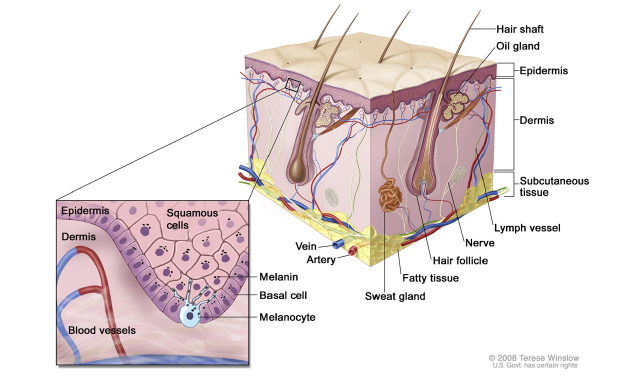
\includegraphics[width = 0.8\textwidth]{Chapter1/Figuers/SkinAnatomy.png}	
	\caption[Skin Anatomy]{Anatomy of the skin, showing the three structure layers of epidermis, dermis and subcutaneous tissue \cite{korotkov2012computerized}.}
		\label{fig:SkinAnatomy}
		\end{figure}	 
\begin{description}
	\item[Epidermis] is the outer layer or surface of the skin. This layer is divided into four sub-layers from top to bottom; stratum corneum, stratum granulosum, stratum spinosum and stratum basal \cite{mcgrath2010anatomy}.

The aforementioned layers contain four types of cells including keratinocytes, melanocytes, Langerhans' cells and Merkel cells. 
The majority of the cells in the epidermis are keratinocytes, the main force for continuous renewal of the skin \cite{mcgrath2010anatomy}.
These cells contain two main attributes of division and differentiation which enable them to renew the outer layer of the epidermis within thirty days.
During this journey, the keratinocytes, which are produced by division of the basal cells (keratinocytes in the basal layer are called basal cells), will move to the next layer while they go through a differentiation process.
Differentiation refers to this morphology and biochemistry transformation of the cells.
At the end of this journey, the keratinocyte cells will lose their nuclie and be transformed to flattened cells filled with keratine.
These cells form the outer most layer of the epidermis (stratum corneum).
At the end of the differentiation process, the corneocytes lose their cohension and separate from the surface in the desquamation process, resulting in renewed skin.

Langerhans' cells are responsible for the detection of foreign bodies (antigens) which invade the epidermis, transporting them to the local lymph nodes, while Merkel cells act as mechanosensory receptors in response to touch, forming close connections with sensory nerve endings \cite{mcgrath2010anatomy}.

Melanocyte cells are found in the basal layer of the epidermis \cite{mcgrath2010anatomy}.
These cells are responsible for distributing packages of melanin pigment, which lead to individual skin and hair colors, to the surrounding keratinocytes.
This chromophore mainly protects the subcutaneous tissue from being damaged by UV radiation.
Whenever the level of UV radiation increases, melanocytes start producing more melanin, resulting in our tanning reaction to sun exposure.
Melanin is the major chromophore of the epidermis which occupies the top 50-100 \si{\micro\meter}, with the exception of superior layers of epidermis.  

In most light propagation models through skin, the sublayers of epidermis are considered as one layer~\cite{lu2000modeling,jolivot2011developpement}.
The epidermal thickness can vary depending on different body parts, however on average, it is usually around 0.1 mm.
The most external sublayer of the epidermis is the stratum corneum.
It is composed of dry dead cells without organelles and is filled with keratin fibres.
Light is absorbed mainly in this layer, due to the epidermis major component melanin.	

\item[Dermis] is the middle layer between the epidermis and the hypodermic layer.
This layer is thicker than the epidermis, with an average thickness of 0.6 to 3 mm \cite{anderson1981optics}. 
The thermoregulation, the mechanical resistance and nourishing of the epidermis are the main functions of this layer. 
The dermis is composed of elastic collagen fibres, blood vessels, nerves, lymph vessels, hair follicles and sweat glands but its principal molecules, with relevant optical properties, are haemoglobin, carotene and bilirubin. 
Haemoglobin is a chromophore of red colour found in the microvascular network of the dermis, typically 100-500 \si{\micro\meter} below the skin's surface. 
This chromophore carries oxygen through vessels and capillaries and accordingly is called oxy-haemoglobin since it contains oxygen and deoxy-haemoglobin. 
The dermis is divided into two sublayers, the papillary dermis with the principal function of thermoregulation and the reticular dermis which gives the skin its strength and elasticity. 

\item[Subcutaneous fat] or hypodermic fat is the deepest layer of the skin, with an average thickness of 4 to 9 mm. 
This layer is composed of connective tissues, fat cells and blood vessels. 

\end{description}

	
% Nevertheless, it is not the aesthetic results of melanocyte activity that draw our attention, but their malignant transformation potential. Although cancer can develop in almost any cell in the body, certain cells are more cancer-prone than others and the skin is no exception. Most skin cancers develop from non-pigmented basal and squamous keratinocytes. Their transformation results in basal cell carcinoma and squamous cell carcinoma, respectively [1, 4]. However, melanocytes that undergo a malignant transformation produce a less common but far more deadly and aggressive cancer: malignant melanoma. The epidemiology and treatment of this cancer, as well as some skin lesions known as its precursors, are described in the following sections.



Cancer can develop in almost any cell in the body. 
However, certain cells are more cancer prone compared to others and the skin is no exception. 
The three most common malignant skin cancers are called basal cell carcinoma, squamous cell carcinoma and melanoma which develop from basal cells, squamous keratinocytes, and melanocytes, respectively. 
Melanocyte cells and their transformation, due to their malignant transformation potential, are our main concern in this thesis. 
Melanoma is less common in comparison to basal cell carcinoma and squamous cell carcinoma.
However, it is the deadliest and most aggressive type of skin cancer. 
The characteristics and treatment of this cancer, as well as some skin lesions very prone to malignancy are described in the following sections.


  %%% Local Variables: 
  %%% mode: latex
  %%% TeX-master: "../thesis"
  %%% End: 
\section{Pigmented Skin Lesions}\label{sec:chp1sec2}

Pigmented skin lesions or melanocytic nevi appear on the surface of the skin~\cite{kaufman2005melanoma}, where the melanocyte cells grow in clusters beside the normal skin cells. 
This is a natural transformation of skin cells and creates benign \ac{psls} such as: 

%\begin{figure}[ht]
%\centering
%		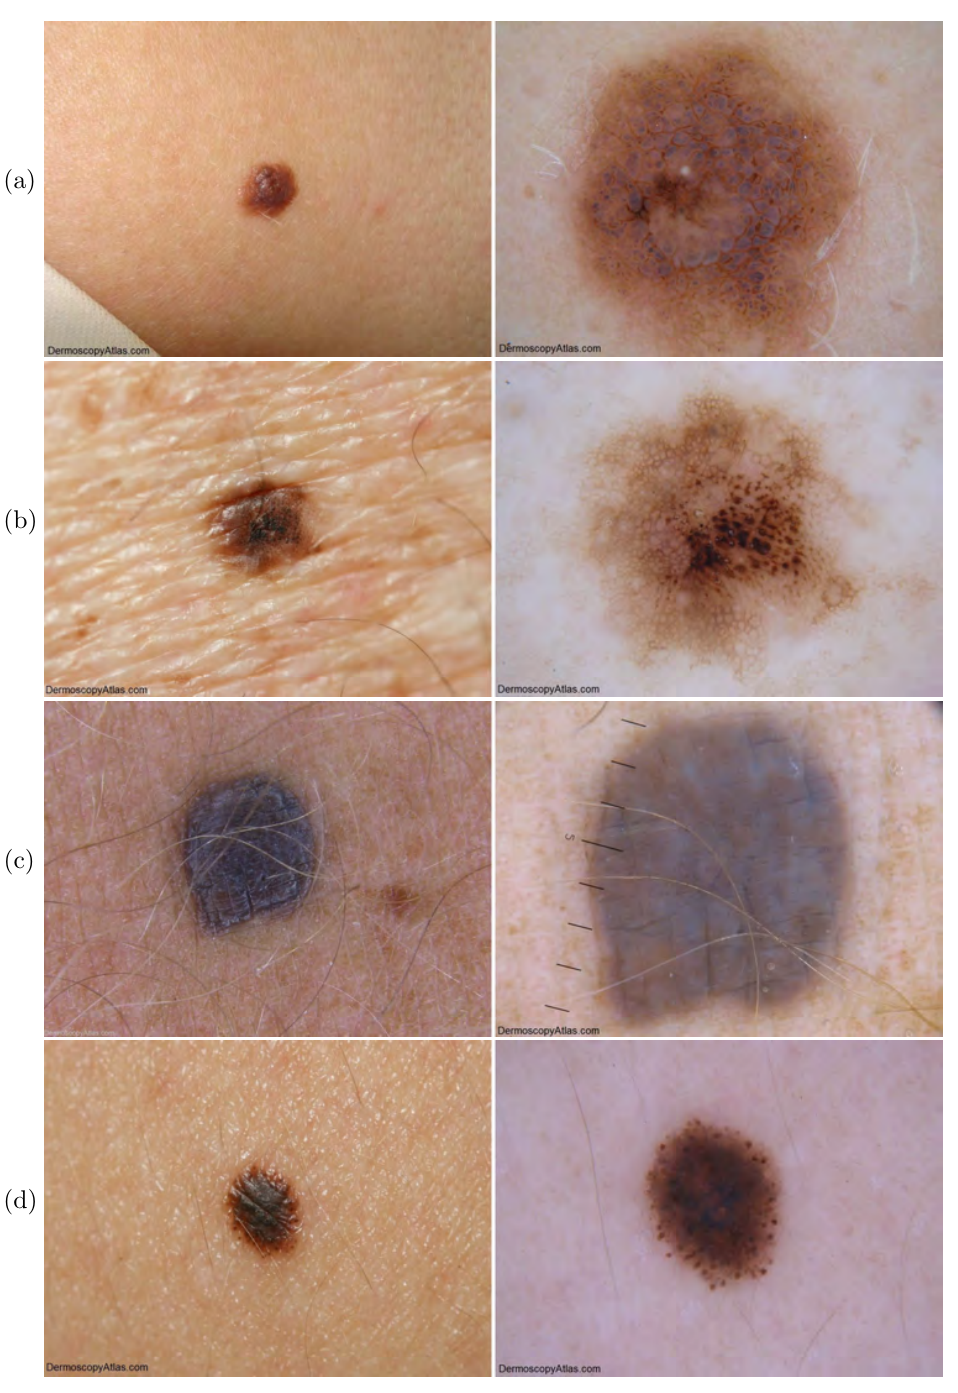
\includegraphics[width = 0.6\textwidth]{Chapter1/Figures/Clinical_DP.png}	
%	\caption{Images of pigmented skin lesions, right column represent the cinical images and left dermoscopy images are presented: (a) congenital nevus; (b) dysplastic nevus; (c) blue nevus; (d) Spitz nevus. {\color{red} ask for permission}}
%		\label{fig:PSLs}
%\end{figure}

\begin{description}
   \item [Freckle] or ephelis are pale-brown macular lesions which are usually of less than 3 \si{\milli\meter} diameter with a poorly defined lateral margin \cite{newton2010lentigos}. 
% which appears and darkens on light-exposed skin sites if  being exposed to ultraviolet
   \item [Common nevi] which are typical flat melanocytic nevi or moles.
   \item [Congenital nevi] which are moles that appear at birth, also known as ``birth marks''.
   \item [Atypical or dysplastic nevi] are common nevi with inconsistent coloration, irregular edges, blurry borders, scale-like texture and a diameter greater than 5 \si{\milli\meter} ~\cite{kaufman2005melanoma}. 
Atypical mole syndrome or dysplastic nevus syndrome, describes individuals with large quantities of dysplastic nevi. 
Such individuals face a higher risk of developing melanoma (6 to 10 times greater than other people with few nevi)~\cite{newton2010lentigos}. 
However, only a small number of these dysplastic nevi might develop into melanoma and most dysplastic nevi will never become cancer.

  \item [Blue nevi] are melanocytic nevi comprised of abnormal collections of benign pigment melanocytes located in the dermis rather than at the dermoepidermal junction~\cite{newton2010lentigos}.
The blue or blue-black appearance of the lesion is caused by light reflection of melanin in the dermis.  
  \item [Pigmented Spitz nevi] are uncommon benign nevi that share a similar physical characteristics to melanoma and are usually seen in children~\cite{newton2010lentigos}. 

\end{description}

From the aforementioned lesions, congenital and dysplastic nevi are most likely to develop into malignant melanoma~\cite{friedman1985early}.  


 
 %%% {I dont know if it is necessary to include this or not} Atypical mole syndrome, also known as “Familial Atypical Multiple Mole Melanoma” (FAMMM) or dysplastic nevus syndrome, describes individuals with large quantities of atypical nevi and possibly inherited melanomas. The relative risk of developing a melanoma in such individuals is around 6 to 10 times that of people with very few nevi [5].



%%% Local Variables: 
%%% mode: latex
%%% TeX-master: "../thesis"
%%% End: 
\section{Malignant Melanoma} \label{sec:chp1sec3}
Although malignant melanoma accounts for less than 2\% of all skin cancer cases, it is the deadliest type and causes the vast majority of deaths \cite{CancerFactsFigures2014}.
The incidence of melanoma has increased in the past few decades currently reaching 132,000 melanoma cases per year according to the \ac{who}. 
%The \Ac{acs} also reported the estimated deaths of melanoma in 2014 as $9710$ individuals and new cases as $76,100$ individuals. 

Melanoma cancer is incurable in its advanced stages and the patient should go through surgery, possibly immunotherapy, chemotherapy, and/or radiation therapy. 
However, if it is diagnosed at an early stage, it is the most treatable kind of cancer~\cite{CancerFactsFigures2014,forsea2012melanoma}.
In fact, patient survival rate has increased significantly, over the past few decades, thanks to early diagnosis and treatment of melanoma in its early stages. 

The stages of melanoma are measured based on how the lesion has grown, including its invasion depth though the skin to nearby lymph nodes or other organs.
This factor is measured through physical exam, biopsies, and different imaging tests such as \ac{ct} or \ac{mri} ~\cite{CancerFactsFigures2014}.
Depending on the measurements obtained, melanoma skin cancers are divided into four types.

The first three types begin \textit{in situ}, meaning that they spread along the top layers of the skin and become invasive in the final stages, while the fourth is invasive from the start.
Invasive melanoma can be very dangerous since they are in the deeper layers of the skin and can spread faster to other body parts. The four types of cutaneous melanoma are listed in the following: 
	\begin{description}
	\item [Superficial spreading melanoma] 
	is the most common type and is the leading cause of cancer death in young adults. 
	Approximately 70\% of all melanoma diagnosis are counted as superficial spreading melanoma. 
	This type grows along the top layer of the skin and often occurs in a previously benign mole. 
	The location of this melanoma can be anywhere in the body, however, it is usually found on the trunk and back in male patients and on the legs and back in females patients.   
	\item [Acral lentiginous melanoma]
	accounts for less than 5\% of all melanoma diagnosis and is the most common type in dark skinned individuals. 
	This disease is usually located on the palms, soles of the feet and under the finger nails and often looks like a bruise or injury on the body.
	For this reason, the melanoma may be discovered later than other forms.  	
	\item [Letingo maligna melanoma]
	accounts for 5-10 \% of melanoma diagnosis. Letingo maligna melanoma arises from a pre-existing letingo rather than a mole and mostly occurs on the face of middle-aged and elderly individuals as a result of sun damage. 
If this cancer goes undiagnosed, being mistaken for a sun spot, it can spread to the deeper layers of the skin and endanger the patient's life. 
Cancer lesions of this type usually have a very irregular border and vary in shades of brown or black.
However, like other types of melanoma, they can be blue, red, gray or white. 
	\item [Nodular melanoma]
	accounts for 15-30\% of all melanoma diagnosis. 
	This is the most aggressive type due to the fact that it spreads more rapidly in depth and it is difficult to visualize the progression of the cancer.
Nodular melanoma is more common in males than in females. 
The lesion is usually darkly pigmented (blue-black) and is often found in pink or red. 
	\end{description}
	
%%% Local Variables: 
%%% mode: latex
%%% TeX-master: "../thesis"
%%% End: 
\section{Melanoma Diagnosis and Screening}\label{sec:chp1sec4}
The clinical prognosis of early stage melanoma is commonly done via visual inspection of the lesions, based on a set of rules or guidelines, such as ``ABCDE''~\cite{abbasi2004early} or Glasgow 7-point checklist~\cite{abbasi2004early}.
The ``ABCDE'' rule characterizes the lesion based on its asymmetry (A), irregular borders (B), variegated colors (C), diameter $\geq$ 6  \si{\milli\meter} (D) and evolving stage over time (E).
The Glasgow 7-point checklist contains 7 criteria: 3 major (changes in size, shape and color) and 4 minor (diameter $\geq$ 7\si{\milli\meter}, inflammation, crusting or bleeding, and sensory change). 
The former rule has been extensively used in clinical routine, rather than the latter one, due to its simplicity.


The visual inspection of lesions is carried out using different non-invasive imaging techniques such as: clinical photography, dermoscopy, \acf{clsm}, \acf{oct}, \acf{msi}, high frequency \acf{us1}, and \acf{mri} among other spectroscopic imaging. 
Concerning the aforementioned techniques, some are well-utilized by clinicians and dermatologists. 
We will refer here and after to these techniques as ``conventional'' techniques.
Clinical photography, dermoscopy, \ac{oct}, and \ac{clsm} belong to this category. 
While the rest, such as \ac{mri}, \ac{us1}, \ac{msi} and \ac{pi} are categorized as ``non-conventional'' techniques.  

We focus our research on conventional techniques such as clinical and dermoscopy as well as non-conventional techniques such as \ac{pi}. 

\subsection{Clinical photography}
Clinical photographs are referred to as digital or non-digital images captured from the surface of the skin, showing one or more lesions. 
These images reproduce what a clinician sees with the naked eye~\cite{day2000automated} and are commonly tainted with unnecessary highlights and reflections from the outer layer of the epidermis. 
The left column of Fig.\,\ref{fig:fig2} shows such images. 
%Breslow thickness 0.8 \si{\milli\meter},
\begin{figure}\centering
\subfloat[In situ melanoma (stage 0)]{
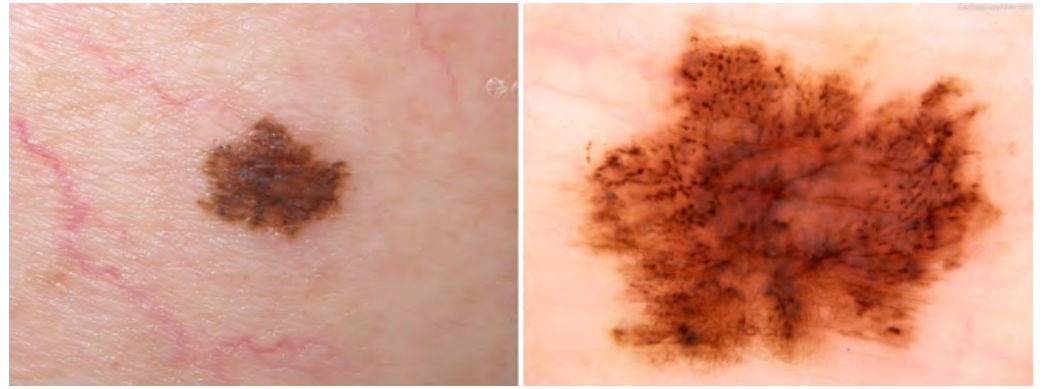
\includegraphics[width = 0.5\textwidth]{Chapter1/Figuers/CD1.png}	}\\
\subfloat[Invasive melanoma ( stage I/II)]{
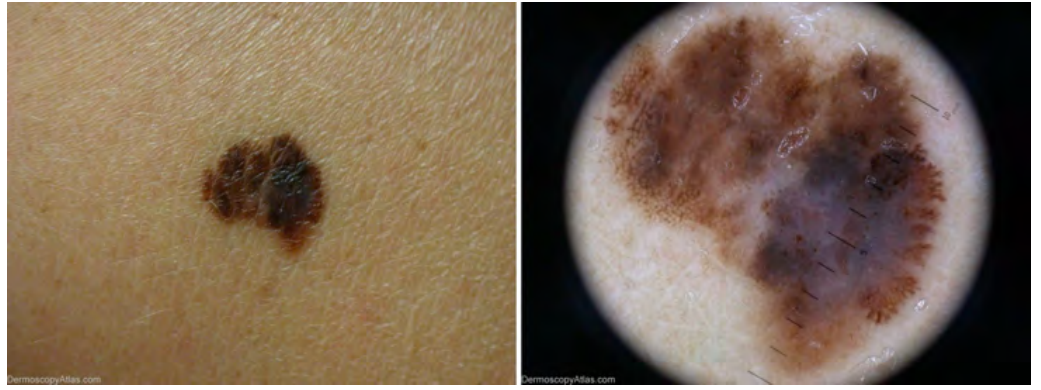
\includegraphics[width = 0.5\textwidth]{Chapter1/Figuers/CD2.png}	}
	\caption[Clinical and dermoscopy images]{Clinical and Dermoscopy images, right and left column, respectively. Images submitted
to www.dermoscopyatlas.com by Dr. Alan Cameron (a), Dr. Jean-Yves Gourhant (b). Used with permission.}
\label{fig:fig2}
\end{figure}

\subsection{Dermoscopy}
\label{subsec:derm}
Dermoscopy (also known as dermatoscopy or epiluminescence microscopy) is a well-established and effective non-invasive technique for early recognition of melanoma. 
This technique, introduced in 1971~\cite{mackie1972cutaneous, mackie1971aid}, uses a hand-held lighted magnifier to analyze skin lesions. 

Initially the device was used in conjunction with a thin layer of glass and an oil or alcohol interface to reduce light reflection, refraction and diffraction.
This material made the epidermis translucent and allowed in vivo visualization of subsurface anatomic structures of the epidermis and papillary dermis which are not visible with naked eye~\cite{rigel2010evolution,wang2010noninvasive}.
This first type of dermoscopes is called a \ac{npd}~\cite{wang2010noninvasive}. 

The second type, the \acf{pd}, was introduced later and made this process much easier by using cross-polarized light. 
This device is equipped with two polarized filters, one in front of the light source and one in front of the sensor. 
The two polarized filters are perpendicular to each other in order to capture the backscattered light from the deeper levels of the skin. 
The light reflected from the skin has the same angle as the polarized incident light, hence it is eliminated with the cross-polarized filter in front of the sensor. 
However, the backscattered light from the skin, due to the structural nature of the tissue, will become unpolarized and passes through the filter.
This technique eliminates the need for fluid or direct contact with the skin.

A sample of commercially available dermoscopes (Dermlite$^{\circledR}$) with and without polarized light are shown in Fig~\ref{fig:fig4}.
MoleMax (Derma Medical System, Vienna, Austria) is another commercially available system that includes a polarized dermoscope.
MoleMax is a computer based device and by providing its own software, allows live-video dermoscopy and total body photography~\cite{marghoob2003instruments,rigel2010evolution}.

\begin{figure}[h]
\centering
\subfloat[Dermlite$^{\circledR}$ II Fluid]{
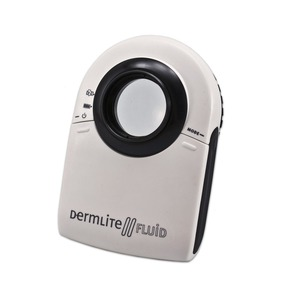
\includegraphics[width = 0.3\textwidth]{Chapter1/Figuers/Dermlite_fluid.jpg}	}
\subfloat[Dermlite$^{\circledR}$ II Pro HR]{
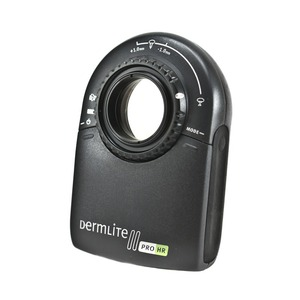
\includegraphics[width = 0.3\textwidth]{Chapter1/Figuers/Dermlite_PD.jpg}	}
\caption[Dermoscopes]{Commercially available dermoscopes by Dermlite$^{\circledR}$:  (a) immersion fluid dermoscope using non-polarized light; (b) cross-polarized light dermoscope. Both devices can be attached to a digital camera.}
\label{fig:fig4}
\end{figure}

The images captured using a \ac{pd} or a \ac{npd} are relatively similar.
However, the surface dermoscopic structures (such as the blue white veil) are better observed with a \ac{npd} while deep structures (such as vessels) are better seen with a \ac{pd}~\cite{wang2010noninvasive, benvenuto2007differences}.
The right column of Fig~\ref{fig:fig2} demonstrates the dermoscopic images of the same lesions captured with an \ac{npd}.
Figure~\ref{fig:fig3} shows difference of clinical, \ac{npd}, and \ac{pd} imaging for a melanoma lesion.

\begin{figure}\centering
\subfloat[Clinical]{
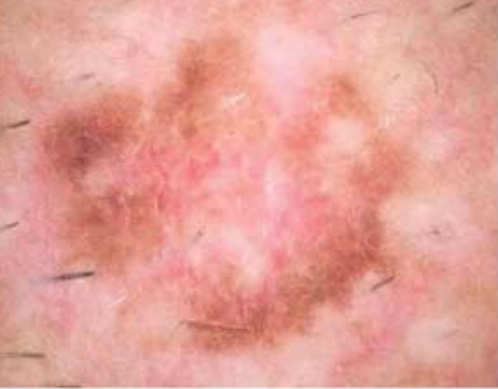
\includegraphics[width = 0.33\textwidth]{Chapter1/Figuers/Melanoma_Clinical.png}}
\subfloat[\ac{npd} ]{
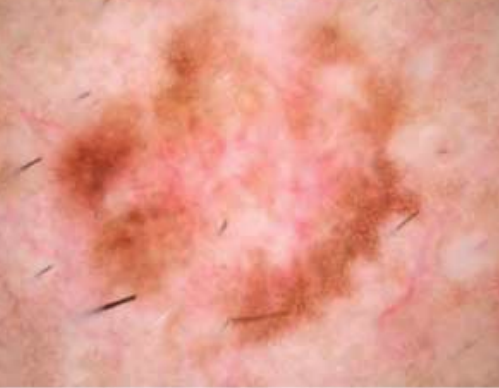
\includegraphics[width = 0.33\textwidth]{Chapter1/Figuers/Melanoma_NPD.png}}
\subfloat[\ac{pd} ]{
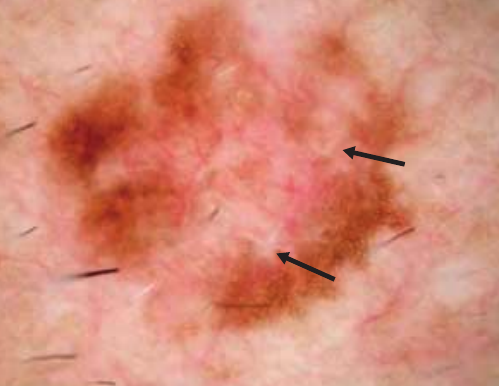
\includegraphics[width = 0.33\textwidth]{Chapter1/Figuers/Melanoma_PD.png}}
	\caption[Clinical, \ac{npd} and \ac{pd} images of melanoma]{Melanoma lesion captured by clinical photography,  An \ac{npd}, and a \ac{pd}, respectively. Shiny white streaks (arrow in (c)) within the melanoma are only visible with the \ac{npd}. The images are taken from Benvenuto~et al.~\cite{benvenuto2007differences}}
\label{fig:fig3}
\end{figure}


Besides the \ac{npd} and the \ac{pd}, another dermoscopy technique, via transillumination, was introduced by Dhawan~et.al.~\cite{Dhawan1985,Dhawan1984}.
In this technique, light is directed to the skin in such a way that allows the backscattered light to illuminate the lesion from within. 
Novescope is a patented device developed for this technique. 
%Figure~\ref{fig:fig5} shows a schematic of this design. The device used for this design is patented and called Nevoscope~\cite{Dhawan1985,Dhawan1984}. 
 


%%% Ask for permission first. 
%\begin{figure}[h]
%\centering
%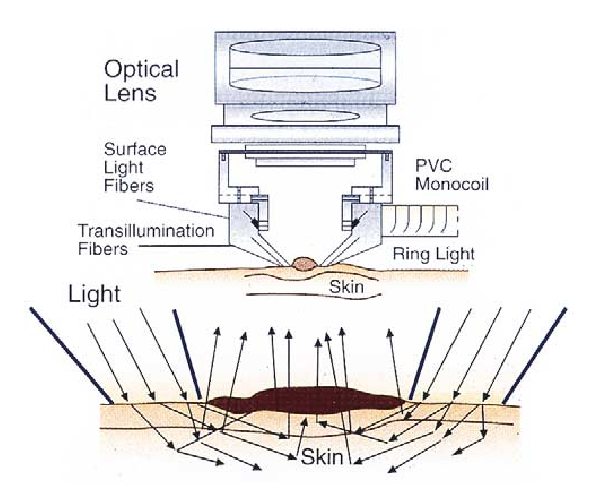
\includegraphics[width = 0.3\textwidth]{Chapter1/Figures/Nevoscope.jpg}	
%\caption{Dermoscopy techniques by transillumination oflesion (Nevoscope)}
%\label{fig:fig5}
%\end{figure}

% for more information the interested reader can refer to : Marghoob 2003, Quintana 2012, L.Smith 2011, Rigel 2010, Wang 2010, Gadeliya 2009, Pstay 2009, Esmaili 2008, Patel 2008  
%\subsection{Confocal Laser Scanning Microscopy}
%\ac*{clsm} is another non-invasive technique, that provides real time in-vivo images of skin at variable depths in horizontal planes equivalent to the resolution of conventional microscope~\cite{rigel2010evolution}. 
%The high resolution of the microscope allows to capture nuclear, cellular, and tissue architectures of the epidermis and underlying structures, without any biopsy.
%In comparison to fluorescence microscopic , the skin is difficult to investigate because it reflects and scatters incoming light and melanin and other chromophores, significantly attenuate visible wavelength. 
%\subsection{Optical Coherence tomography}

\subsection{Polarized imaging}
In \acf{pi} or image polarimetry systems a polarizer state generator and analyzer are used to create a set of polarized images. 
These images define the polarization state of the light beam and the depolarization property of the tissue.
The former is represented by four measurable quantities called Stokes parameters and the later is represented by the Mueller matrix. 
The advantage and benefits of \ac{pi} systems besides being cross-polarized are not as evident in the field of skin imaging or tissue imaging in general.
Over the last few decades, few studies have been dedicated to finding and exploring the depolarization properties of tissues~\cite{Anastasiadou2008,manhas2009polarized,manhas2009polarized,Jacques12175282}
%Anastasiadou~et al.\ proposed a Mueller polarimetry system for diagnosing the cervical cancer \cite{Anastasiadou2008} and Manhas~et al.\ proposed a Mueller polarimetry system for measuring polarized diffuse reflectance on cancerous and non-cancerous regions of oral cavity and breast tissues \cite{manhas2009polarized}. 
%In the field of skin tissue, Jacques~et al.\ proposed Stokes polarimetry to differentiate different pigmented lesions \cite{}. 
%Another work recently was proposed by Tchvialeva~et al.\ where polarized speckle imaging was suggested for in vivo screening of pigmented lesions \cite{manhas2009polarized}. 
The Stokes and Mueller measurements along with the basics of polarization and the methods proposed by the research community are further explained in Chap.\,\ref{chp:chapter4}
%The Stokes polarimetry, Mueller matrix measurements, and the proposed methods by the research community are further explained in Chapt.\,\ref{chp:chapter4}.


%\subsection{Multispectral Imaging}
%In multispectral imaging, a set of wavelength dependent images are acquired in order to visualize different depths and layers of the skin. 
%This is possible since depth of light penetration into the skin is directly related to wavelength. 
%The wavelengths can range from \ac{uv} to \ac{nir}. 
%This technique offers the advantage of analyzing the sub-layers which are not visible to the human eye, probing up to 2 \si{\milli\meter} below the surface of the skin~\cite{rigel2010evolution}~(see Fig.~\ref{fig:MSI_ex1}).

%\begin{figure}[h]\centering
%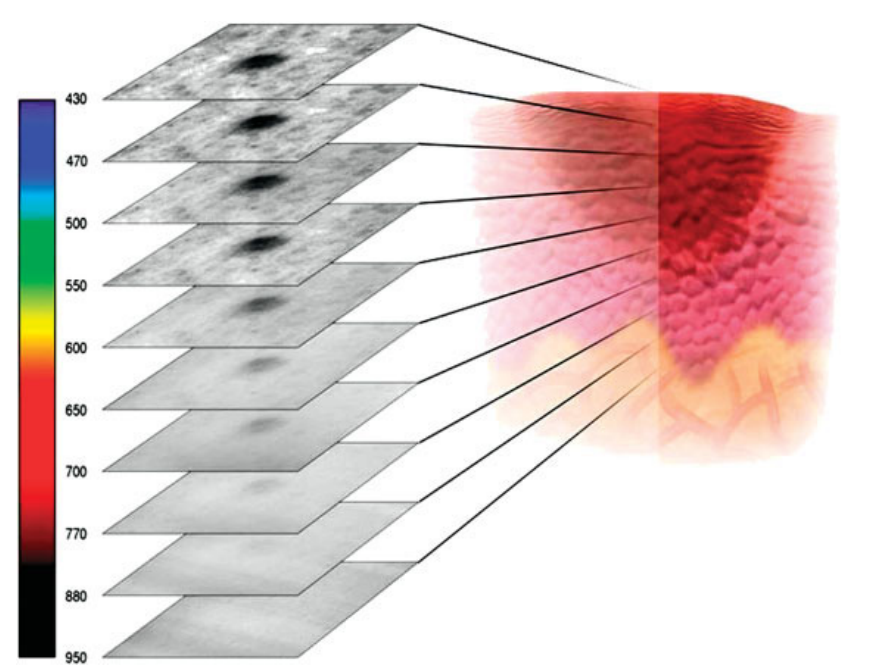
\includegraphics[scale=0.5]{Chapter1/Figuers/MS_example.png}
%\caption[Multispectral analysis of pigmented skin lesions]{Multispectral analysis of pigmented skin lesion. Longer wavelength penetrates deeper into the skin, providing diagnostic features. The image is taken from Rigel~et al.~\cite{rigel2010evolution} }
%\label{fig:MSI_ex1}
%\end{figure} 
%Opposed to standard color cameras which capture the skin image in three channels (red, green, blue), \ac{msi} acquires a sequence of gray level images at different wavelengths. 
%This extended spectral capacity provides a high advantage in skin imaging since it is reducing the effects of metameric mismatches, which may occur due to different illumination and variability of sensor spectral responses \cite{jolivot2011developpement}.
%The spectral device of \ac{msi} can be placed either along the incident path, or in detection path.
%In either way, the main motivation is to go beyond the limited red, green and blue color information which are available by other imaging techniques. 
%This technique combines the advantage of both a spectrophotometer and a digital camera. 
%The \ac{msi} system acquires three-dimensional data, the spatial information in 2 dimensions and a spectral information in the third dimension, obtaining spectral information for each pixel in the image. 	
%	
%Currently, several multispectral dermoscopes are commercially available: MelaFind~\cite{elbaum2001automatic,Gutkowicz-Krusin1997}, SolarScan~\cite{menzies2001short,menzies2005performance}, and SIAscope~\cite{moncrieff2002spectrophotometric}. 
%This topic is extensively discussed in Chapt.\,\ref{chp:chapter5}.





  %%% Local Variables: 
  %%% mode: latex
  %%% TeX-master: "../thesis"
  %%% End
\section{Automated Diagnosis of Melanoma}
\Ac{cad} or \ac{cds} systems are proposed to provide automated diagnosis of melanoma lesions. 
These systems are intended to reproduce the decision of the dermatologists when observing images of \ac{psls}. 
Automated diagnosis of melanoma was proposed to assist dermatologists and increase the sensitivity and specificity of melanoma recognition in their early stages as well as to reduce unnecessary excisions.
From a computer vision and pattern recognition point of view, \ac{cad} systems for melanoma intend to classify and differentiate melanoma lesions from others.
In general, image processing techniques are used to locate and delineate the lesions and extract the image parameters (features) which coincide with the dermatologist's point of view and dermatological features. 
The extracted parameters are further used with machine learning tools to perform a diagnosis (classification). 
Such systems are being developed for various imaging modalities~\cite{Marchesini2002,Vestergaard2008,korotkov2012computerized}. 
However, dermoscopy being the most conventional imaging technique, most \ac{cad} systems are dedicated to this modality. 
%This research is aimed to provide an automate classification framework of melanoma lesions based on conventional dermoscopy and non-conventional \ac{pi}.

This research is aimed at analyzing the effects of polarized illumination beyond that of usual dermoscopes, for the detection of melanoma lesions and providing a \ac{cad} system for an automated classification of melanoma lesions based on conventional dermpscopes and image polarimetry.
%In our research, we considered automated classification of melanoma based on conventional dermoscopy, and non-conventional \ac{msi} and \ac{pi} imaging.  
The general steps of a \ac{cad} system are extensively discussed in Chap.\,\ref{chp:chapter2}.

\subsubsection{Clinical impact}
Numerous research projects have been dedicated to the development of a \ac{cad} or \ac{cds} system and studies show that their performance is sufficient under experimental conditions~\cite{Fruhauf2012}. 
The proposed systems can assist dermatologists, however, their practical value is still unclear and they cannot be recommended as a sole determinant of malignancy of a lesion.
Even though most patients would accept a computerized analysis of a melanoma, the \ac{cad} systems proposed cannot function alone due to their tendency to over diagnose benign melanocytic and non-melanocytic lesions~\cite{Fruhauf2012}.
Day and Barbour~\cite{Day2001} listed two main shortcomings for general approaches which are adapted to develop a \ac{cad} system for recognition of a melanoma:
\begin{enumerate}
\item A \ac{cad} system is expected to reproduce the decision of pathologists (a binary result like ``melanoma/non-melanoma lesion'') with only the input used by dermatologists: clinical or dermoscopic images;
\item Histopathological data are not available for all lesions, only for those considered suspicious by dermatologists.
\end{enumerate}
\noindent
The items listed refer to the lack of sufficient information and interaction with dermatologists used in the proposed method.
These items refer to the fact that the proposed methods lack sufficient information and interaction with dermatologists.
This fact was highlighted by Dreiseitl~et al.\,\cite{Dreiseitl2005} as well. 
The authors mentioned that current systems are designed to work ``in parallel with and not in support of'' physicians, thus only a few systems have been used in clinical routines.
In this regard, an ideal \ac{cad} or \ac{cds} system for melanoma recognition should be able to reproduce the dematologists's decision with extensive information regarding the reason and ground for that decisions~\cite{Dreiseitl2005}.

\section{Research Motivation}
\label{sec:chp1sec6}
Malignant melanoma is the deadliest type of skin cancer and accounts for the vast majority of skin cancer deaths~\cite{CancerFactsFigures2014}.
According to the latest reports, melanoma causes over 20,000 deaths annually in Europe~\cite{forsea2012melanoma}.
The \Ac{acs} also reported an estimated deaths of melanoma in 2014 as $9710$ individuals and new cases as $76,100$ individuals~\cite{CancerFactsFigures2014}.
Nevertheless, melanoma is the most treatable kind of cancer if diagnosed early.
Therefore, prevention and early diagnosis of melanoma lesions is crucial for the patients survival rate.

\acl{cad} systems have been proposed by the research community to assist dermatologists in early diagnosis of melanoma.
These systems are proposed to classify \acf{psls}.
Dermoscopy being the most common source of skin imaging, most of the \ac{cad} systems proposed are based on polarized dermoscopy (PD).
The \ac{pd} allows the visualization of the subsurface anatomic structure of the epidermis and papillary dermis.
Although \ac{pd} are used extensively by the dermatologist to document and analyze the \ac{psls}. 
The advantage and benefits of \acf{pi} beyond the cross-polarized filters, have not been fully explored in the field of skin cancer.

This work attempts to analyze more closely \ac{pi} in the field of skin cancer and intends to propose an automatic classification framework based on dermoscopy and image polarimetry.
For this purpose, a novel image polarimetry system able to provide the first three Stokes parameters is presented.
This system is implemented based on Stokes polarimetry since it can provide automatic, fast, accurate and less complex acquisition, in comparison to Mueller polarimetry. 

Towards providing a \ac{cad} system, different aspects of automated classification of \ac{psls} are extensively investigated and a \ac{cad} system based on dermoscopy images is proposed. 
Further using the proposed image polarimetry system, polarization properties of the \ac{psls} are analyzed and a \ac{cad} system based on new polarized features is presented.



\section{Thesis Outline}
\label{sec:chp1sec7}
This thesis describes the research work that resulted in the development and validation of the Stokes polarimetry device and a classification frameworks for differentiation of melanoma using conventional cross-polarized and non-conventional image polarimetry techniques. 

Prior to developing a polarimetry system and a \ac{cad} framework, the basics and principles of polarization and classification frameworks are explored.
The basics of polarization and a history of polarimetry images is presented in \textbf{Chapter~\ref{chp:chapter4}} while \textbf{Chapter~\ref{chp:chapter2}} discuss the related machine learning and computer vision techniques related to the classification framework.
%Since classification is the base of our \ac{cad} systems, related machine learning and computer vision techniques are discussed in \textbf{Chapter~\ref{chp:chapter2}}. 

\textbf{Chapter~\ref{chp:chapter3}} is dedicated to dermoscopy modality. 
State of the art of \ac{cad} systems, our proposed framework, experiments and results obtained for dermoscopy modality are depicted in this chapter. 

\textbf{Chapter~\ref{chp:chapter5}} presents the framework developed for the \ac{pi} modality. 
The \Ac{pi} system and the developed classification framework along with the results obtained are presented in this chapter. 

Finally \textbf{Chapter~\ref{chp:chapter6}} concludes the thesis and presents avenues for future research.

%Additional information on the techniques used in the implementation of the PSL mapping and change detection pipelines can be found in the \textbf{Appendix}. %~\ref{sect:appendixA}}.
	



%%% Local Variables: 
%%% mode: latex
%%% TeX-master: "../thesis"
%%% End: 

\clearemptydoublepage
\acresetall
\chapter{Polarization Principles and Image Polarimetry}
\label{chp:chapter4}

%\section{Introduction}\label{sec:chp4-sec1}
Light was thought as being non-scalar for the first time by Christian Huygens when he observed the propagation of light through crystals~\cite{goldstein2003polarized}.
Through observations it appeared that light had ``sides'', in the words of Newton.
This new vectorial nature of light was called polarization.
Later, Frensel and Arago discovered that light consisted of only two transverse components and the perpendicular components were assumed to propagate in the $z$ direction.
%The light was suggested for the first time to be non scalar by Christian Huygens when he observed the propagation of light through crystals. It appeared that light had "sides" in the words of Newton. The new vectorial nature of light is called polarization. Later Fresnel and Arago discovered that light consisted only of two transverse components. The components are perpendicular to each other and are assumed to propagate in $z$ direction. 

The concept of polarization arises from the transverse and vector nature of electromagnetic radiation.
This concept describes the resultant pattern of an electric field vector ($E(r,t)$) as a function of time ($t$) at a fixed location in space ($r$).
The classical theory of polarization and the nature of light are evidence that polarization is another fundamental property of light besides coherent, frequency and intensity.

%This chapter is organized such as, first polarized properties of light and the mathematical representation of these properties are presented, then the polarized properties of the medium and it's mathematical formulations are explained and finally the related works on image polarimetry systems are discussed.
In this chapter, the polarized properties of light and the mathematical representation of these properties are explained first.
This section focuses on the mathematical formulations used in dermopolarimetry. 
Later the polarized properties of the medium and it's mathematical formulations through the Stokes representation are presented and, finally, the related work on image polarimetry systems are explained.



%Finally we discuss the image polarimetry systems proposed by the research community.
% This chapter is organized such as, first the basic and principals of polarization are discussed, then the image polarimetry and related works to this filed are presented.
%\section{Polarization}
\section{Polarization Properties of Light}\label{sec:chp4-sec2}
The propagation of the optical field in the isotropic medium is described using three independent waves.
%Three independent waves are required to describe the propagation of the optical field in isotropic medium.
\begin{equation} 
\small
 	\nabla^{2} u_{i}(r,t) = \frac{1}{\nu^{2}}\frac{\partial^{2}u_{i}(r,t)}{\partial t^{2}}~,  \hspace{1cm}   i = x, y, z 
\label{eq:eq1}
\end{equation}
\noindent In Eq.~\ref{eq:eq1}, $\nu$ is the velocity of the oscillation and $r = r(x,y,z)$ defines a point in the Cartesian system.
In this system, $u_{x}(r,t)$ and $u_{y}(r,t)$ are called transverse components and $u_{z}(r,t)$ is the longitudinal component of the optical field:
\begin{subequations} \label{eq:eq2}
\small
	\begin{align}
 		u_{x}(r,t) =  u_{0x} \cos(\omega t - k . r + \delta_{x})~,\\
 		u_{y}(r,t) =  u_{0y} \cos(\omega t - k . r + \delta_{y})~,\\
 		u_{z}(r,t) =  u_{0z} \cos(\omega t - k . r + \delta_{z})~. 
 	\end{align}
\end{subequations}
 
In 1818, Fresnel and Arago carried out several experiments and concluded that the longitudinal component of light does not exist: in another words, light only contains transverse components.
By assuming the direction of propagation in the $z$ direction, the transverse components of the Eq.~\ref{eq:eq2} are reformulated by Eq.~\ref{eq:eq3}, where $\tau = \omega t - kz$ is the propagator, $E_{0x}$ and $E_{0y}$ are the maximum amplitude and $\delta_{x}$ and $\delta_{y}$ are the time independent phases of the two transverse components.

 \begin{subequations} \label{eq:eq3}
 \small
\begin{align}
 	E_{x}(z,t) = E_{0x} \cos(\omega t - kz+ \delta_{x})= E_{0x} \cos(\tau + \delta_{x})~,\\
 	E_{y}(z,t) = E_{0y} \cos(\omega t - kz + \delta_{y}) = E_{0y} \cos(\tau + \delta_{y})~.
 \end{align}
\end{subequations}
 
Transverse waves of light are said to be ``instantaneous'' since, at optimal frequencies, the time for a wave to go through one complete cycle is only \SI{e-15}{\second} \cite{goldstein2003polarized,2006opma.book.....T}.
Due to this feature, the electrical field vector is the result of two waves tracing a single curve almost instantaneously.
The theoretical case of this curve is an ellipse (Polarization ellipse) when $\delta = \delta_{x} - \delta_{y}$ is constant over time.
Equation\,\ref{eq:eq4} presents the formulation of the curve and the polarization ellipse.  

\begin{equation}\label{eq:eq4}
\small
 	\frac{E_{x}^2}{E_{0x}^2} + \frac{E_{y}^2}{E_{0y}^2}-2\frac{E_{x}E_{y}}{E_{0x}E_{0y}}\cos \delta = \sin^2 \delta    \hspace{1cm} (\delta = \delta_{y} - \delta_{x})~.
\end{equation}
 
Figure.~\ref{fig:PolEllipse} represents this ellipse bounded by a rectangle.
The sides of this rectangle are parallel to the coordinate axes of the ellipse with lengths of $2E_{0x}$ and $2E_{0y}$ respectively.
This ellipse is tangent to the sides of the rectangle at four points ($A, B, C, D$).
The formulations of these points are represented by Eq.~\ref{eq:eq5}, and Eq.~\ref{eq:eq6} shows the calculation of the polarized ellipse area. 
\begin{figure}
 \centering
 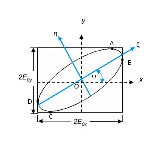
\includegraphics[width = 0.4\textwidth]{Chapter4/Figures/polellipse.eps}
 \caption{An elliptically polarized wave and the polarization ellipse.}
 \label{fig:PolEllipse}
\end{figure}
 
\begin{eqnarray}\label{eq:eq5}
\small
 	A: +E_{0x} \cos\delta,  +E_{0y} \hspace{1cm}
 	B: +E_{0x},  +E_{0y}\cos\delta \\ \nonumber
 	C: -E_{0x} \cos\delta, -E_{0y}\ \hspace{1cm}
 	D: -E_{0x},  -E_{0y}\cos\delta 	
\end{eqnarray}
\begin{equation}\label{eq:eq6}
	\textit{A} = \pi E_{0x}E_{0y}\sin\delta~.	
\end{equation}

\noindent Different values of $E_{0x}$, $E_{0y}$, and $\delta$ form various shapes of polarized ellipse and create different states of polarized light, including;

\begin{itemize}
	\item \textbf{Linearly horizontal / vertical polarized light}\\
	 When one of the transverse components does not exist ($E_{0y}$ = 0 or $E_{0x}$ = 0), oscillation happens in one direction only ($x$ or $y$ respectively).
	 The oscillation in $x$ direction is called linearly horizontal polarized and in the $y$ direction, linearly vertical polarized light.  
	\item \textbf{Linear $+45^{\circ}$ / $-45^{\circ}$ polarized light}\\
	 When $\delta = 0$ or $\pi$, Eq.~\ref{eq:eq4} is formulated by Eq. \ref{eq:eq7}.
	 In this form, light is linearly polarized with a slope of $\pm E_{0y} / E_{0x}$.
	 In this case, if $E_{0x} = E_{0y}$, the light is said to be linearly $+45^{\circ}$ polarized for parameter $\delta = \pi$ and linearly  $-45^{\circ}$ polarized for $\delta = 0$. 
	 \begin{equation}\label{eq:eq7}
	 \small
	 	E_{x} = \pm (\frac{E_{0y}}{E_{0x}})E_{y}~.
	 \end{equation}	 
	 \item \textbf{Left / right circular polarized light}\\
	When $\delta = \pi/2$ or $3\pi/2$, Eq.~\ref{eq:eq4} indicates the identical standard equation of the ellipse.
	In this condition, if $E_{0x} = E_{0y} = E_{0}$, the ellipse transforms into a circle and the light is said to be circularly left polarized ($\delta = \pi/2$) or circularly right polarized ($\delta = 3\pi/2$).
	\item \textbf{Un-polarized light}\\
	When the phase difference $\delta$ is unpredictable and rapidly varies in time, the light is said to be un-polarized.
	In this case, there is no particular polarization direction and the electrical field is equally distributed in all directions.
	 \end{itemize} 

Besides amplitudes and phase differences, a polarization ellipse contains two other elliptical parameters, the angle of rotation $\psi$ and the ellipticity angle $\chi$.
These two parameters are defined using the angle $\alpha$.
This angle is defined as $\tan(\alpha) = E_{0y}/E_{0x}$, where $\alpha$ is within the limits of $ 0\leq \alpha \leq \pi/2$.
Using this definition, the rotation and ellipticity angle of an ellipse is formulated as: 
\begin{subequations}\label{eq:eq8}
\small
	\begin{align}
	\tan 2\psi = \frac{2E_{0x}E_{0y}\cos\delta }{E_{0x}^{2}-E_{0y}^{2}} = (\tan 2\alpha) \cos\delta  \hspace{2 cm}  0\leq \psi \leq \pi~, \\
	\sin 2\chi =\frac{2E_{0x}E_{0y}\sin\delta }{E_{0x}^{2}+E_{0y}^{2}}= (\sin 2\alpha) \sin\delta  \hspace{1 cm}   -\pi/4\leq \chi\leq \pi/4~.
	\end{align}
\end{subequations}

The handedness of the elliptical polarization state can be defined using the sign $\chi$.
If $\chi$ is negative, then  $\delta$ is also negative and the field rotates counter-clockwise (from $x$ to $y$) which leads to a left handed orientated elliptical state.
On the other hand, if $\chi$ is positive, the polarization state is orientated to the right.

%\section{Stokes Parameters}\label{sec:chp4-sec3}
%Characteristics of the polarized light are explained with different formulations, such as Stokes parameters, Mueller matrix, Jones matrix, and Pincor\'e sphere.
%The full explanation of all these formulations are beyond our scope and we limited our explanations to Stokes and Mueller characteristics.


\section{Stokes Parameters}\label{sec:chp4-sec3}
In 1852, Sir George Gabriel Stokes discovered that polarization behavior could be represented in terms of observables.
Sir.~Stokes in an attempt to mathematically characterize un-polarized light, defined un-polarized light as light whose intensity is unaffected when a polarizer is rotated or while a retarder of any retardance value is present. 
In this characterization Sir~Stokes defined four measurable quantities known as  the Stokes polarization parameters. (See Eq.\ref{Eq:Stokeseq}).
\begin{equation}\label{Eq:Stokeseq}
\small
	(E_{0x}^{2}+ E_{0y}^{2})^{2} - (E_{0x}^{2}- E_{0y}^{2})^{2}- (2E_{0x}E_{0y}\cos\delta)^{2} =  (2E_{0x}E_{0y}\sin\delta)^{2}~,
\end{equation}
The first parameter expresses the total intensity of the optical field in terms of the total amount of horizontal and vertical linear polarization.
The second and third parameters describe the amount of linearly polarized light and the fourth parameter describes the amount of left or right circularly polarized light.
The total \acf{dop}, the \acf{dolp} and the \acf{docp} are calculated using Stokes parameters.
Equation.~\ref{Eq:stokevector} represents the Stokes vector with the parameters represented first in terms of amplitudes of the transverse components ($E_{0x}, E_{0y}$) and  $\delta$ angle, then using different states of polarization.
Here $I_{H}$ and $I_{V}$ stand for linear horizontal and vertical polarized, respectively and $I_{P}$, $I_{M}$, $I_{L}$, $I_{R}$ represent linear $+45^{\circ}$, linear $-45^{\circ}$, left circular and right circular polarized light, respectively. 

\begin{equation}\label{Eq:stokevector}
\small
S = 
	\begin{bmatrix}
	S_{0}\\
	S_{1}\\
	S_{2}\\	
	S_{3}\\
	\end{bmatrix} 
	= 
	\begin{bmatrix}
	I\\
	Q\\
	U\\	
	V\\
	\end{bmatrix} 
	= 1/2
	\begin{bmatrix}
	E_{0x}^{2} + E_{0y}^{2} \\
	E_{0x}^{2} - E_{0y}^{2}\\
	2E_{0x}E_{0y}\cos\delta\\	
	2E_{0x}E_{0y}\sin\delta\\
	\end{bmatrix} 
	= 
	\begin{bmatrix}
	I_{H}+ I_{V}\\
	I_{H}- I_{V}\\
	I_{P}- I_{M}\\
	I_{L}- I_{R}\\
	\end{bmatrix}~.	
\end{equation}

The four Stokes parameters are real quantities in terms of intensities and, for any state of polarized light, they always satisfy the relation shown in Eq.~\ref{Eq:Stokesineq}.
The equality sign applies when completely polarized light exists and inequality applies when partially polarized light or un-polarized light exists.
\begin{equation}\label{Eq:Stokesineq}
\small
	S_{0}^{2}\geqslant S_{1}^{2}+ S_{2}^{2}+S_{3}^{2}~.
\end{equation}

As mentioned above, the first element of the Stokes vector represents the total intensity of light.
The \ac{dop} of light is defined as the ratio of polarized intensity per total intensity.
In a similar manner, \ac{dolp} and \ac{docp} are calculated.
\begin{subequations}\label{Eq:DP}
\small
	\begin{align}
	\ac{dop}  & =  \rho =\frac{I_{pol}}{I_{tot}} = \frac{(Q^2 + U^2 + V^2)^{1/2}}{I}~, \\
	\ac{dolp} & = \rho_{l}= \frac{(Q^2 + U^2 )^{1/2}}{I}~, \\
	\ac{docp} & = \rho_{c} = \frac{V}{I}~.
	\end{align}
\end{subequations}

With respect to Eq.~\ref{eq:eq8}, the relation between rotation and the ellipticity angle of the polarized ellipse and Stokes parameters are defined by: 

\begin{equation}\label{Eq:ellipparStokes}
\small
	\sin 2\chi = S_{3}/S_{0}   \hspace{1.5cm} \tan 2\psi = S_{2}/S_{1}~.
\end{equation} 
\noindent With regard to Eq.~\ref{Eq:ellipparStokes}, the Stokes representation in terms of rotation, the ellipticity angle and $\alpha$ is given by: 

\begin{equation}\label{Eq:nrStokesvec}
\small
S = 	 S_{0}
	\begin{bmatrix}
	1 \\
	\cos 2\chi \cos 2\psi\\
	\cos 2\chi \sin 2\psi\\	
	\sin 2\chi
	\end{bmatrix} 
	= I_{0}
	\begin{bmatrix}
	1\\
	\cos 2\alpha \\
	\cos 2\alpha \cos\delta\\	
	\sin 2\alpha \sin\delta
	\end{bmatrix}~.
\end{equation}

Table~\ref{tab:chp4T1} illustrates polarization states and their relative Stokes vector.
\begin{table}
\small
\begin{center}
\caption{Stokes vector for polarization states.}
\resizebox{1.0\linewidth}{!}{
\begin{tabular}{c c c c c c c c }
    \hline
   & & & & & & & \\[-2.5ex] 
   Polarization states & H & V & $+45^{\circ}$ & $-45^{\circ}$ & R & L & Elliptical\\
   & & & & & & &  \\[-2.5ex] 
   \hline
   &   & & & & & & \\[-1.5ex]
   Stokes Vector  &  &   &   &  &  & & \\
   $\begin{bmatrix}
    S_{0}\\ S_{1}\\ S_{2}\\ S_{3}    
   \end{bmatrix}$ &    
   $\begin{bmatrix}
   1\\ 1\\ 0\\ 0    
   \end{bmatrix}$& 
   $\begin{bmatrix}
   1\\  -1\\  0\\  0    
   \end{bmatrix}$& 
   $\begin{bmatrix}
   1\\ 0\\ 1\\ 0    
   \end{bmatrix}$& 
   $\begin{bmatrix}
   1\\ 0\\ -1\\ 0    
   \end{bmatrix}$&  
   $\begin{bmatrix}
   1\\ 0\\ 0\\  1   
   \end{bmatrix}$&    
   $\begin{bmatrix}
   1\\ 0\\ 0\\ -1    
   \end{bmatrix}$& 
   $\begin{bmatrix}
	1 \\
	\cos 2\chi \cos 2\psi\\
	\cos 2\chi \sin 2\psi\\	
	\sin 2\chi 
   \end{bmatrix}$\\
    &  &  &  &  &  &  & \\
    \hline   
  \end{tabular}
  }
  \label{tab:chp4T1}
  \end{center}
\end{table}
There are different ways of measuring Stokes parameters. 
A classic way of measuring these parameters is by passing an optical beam through two optical elements, known as the retarder and the polarizer.
The retarder is an element that changes the phase between two transverse components of the light, and the polarizer is an element that changes the amplitude of the transverse components.
The incident light passes through the retarder which then advances the phase of the $x$ component ($E_{x}$) by  $\phi/2$ and retards the phase of the $y$ component by $\phi/2$. 
The beam merging from the retarder (the phase shifting element) passes through the polarizer next.
The polarizer has the ability to transmit the optical field through only one axes called the transmission axis. 
For instance, if the transmission axis of the polarizer is at $\theta$, only the $E'_{x}$ and $E'_{y}$ components in this direction pass through.

Using this set-up, the first three Stokes parameters are measured by removing the retarder and rotating the transmission axis of the polarizer to the angles $\theta = 0^{\circ}, \theta = +45^{\circ}$ and $\theta = +90^{\circ}$, respectively.
For measuring the final parameter, a retarder is added to the set-up with the angle of $\phi = 90^{\circ}$ (quarter-wave retarder), while the transmission axis of the polarizer is set to $\theta = +45^{\circ}$.
Equation.~\ref{Eq:cStokesmeas} represents how this set-up can be used to measure the Stokes parameters.
$I(\theta, \phi)$ shows the intensity produced by the retarder with a $\phi$ phase shift angle and the polarizer with its transmission axis at $\theta$.

 \begin{subequations}\label{Eq:cStokesmeas}
 \small
% \begin{center} 
 	\begin{align}
 	S_{0} & =  I(0, 0) + I(90,0)~, \\
 	S_{1} & =  I(0,0) - I(90,0)~, \\
 	S_{2} & = 2I(45,0)-I(0,0)-I(90,0)~,\\
 	S_{3} & = 2I(45,90) - I(0,0) -I(90,0)~. 
	\end{align} 
 %\end{center}
 \end{subequations}




\section{Optical Properties of Medium}\label{sec:chp4-sec4}

Besides the nature of the light and polarized states of incident light, we are interested in checking the polarized properties of the optical elements and subjected materials.
In this regard, this section is dedicated to describing the optical properties of the medium and their formulation.
%Mueller matrix is used to describe the transfer function and interaction of any medium with polarized light.
%In the previous section, we explained the polarization state of the the light through Stokes parameters.
%In this section, we describe the transfer function and interaction of any medium with polarized light using Mueller matrix. 
%%In this section, we present the Mueller matrix which describes the transfer function of any medium in its interaction with polarized light.

\subsection{Mueller matrix parameters}
\label{subsec:MuellerMeasurement}
%In the previous section, we explained the polarization state of the the light through Stokes parameters.
%In this section, we describe the transfer function and interaction of any medium with polarized light using Mueller matrix. 
%%In this section, we present the Mueller matrix which describes the transfer function of any medium in its interaction with polarized light.
The Mueller matrix is used to describe the transfer function and interaction of any medium with polarized light.
The $4 \times 4$ Mueller matrix was invented by Hans Mueller in the 1940s~\cite{goldstein2003polarized}.
If the incident polarized beam interacts with a polarizing medium, its elements will change, so the emerging Stokes vector is as shown in Eq.~\ref{Eq:Meuller1}.

\begin{equation}\label{Eq:Meuller1}
\small
	\begin{bmatrix}
	S_{0}\\S_{1}\\S_{2}\\S_{3}
	\end{bmatrix} = 
	\begin{bmatrix}
	m_{11} & & m_{12} & & m_{13} & & m_{14}\\m_{21}& & m_{22}& & m_{23}& & m_{24}\\m_{31}& & m_{32}& & m_{33}& & m_{34}\\m_{41}& & m_{42}& & m_{43}& & m_{44}
	\end{bmatrix}
	\begin{bmatrix}
	S'_{0}\\S'_{1}\\S'_{2}\\S'_{3}
	\end{bmatrix}~.
\end{equation}

After interaction with the medium, the polarization state of the optical beam can change in terms of:
%The polarization state of optical beam always will change after interacting with matter, these changes could be seen as: 
\begin{itemize}
\item Amplitude of the polarization state
\item Phase of the polarization state
\item Direction of the orthogonal field components
\item Energy of the polarized and un-polarized states by transferring energy between them. 
\end{itemize}

The optical device that changes the amplitude of the transverse components of an optical beam is called a \textit{polarizer} or \textit{diattenuator} and the optical element that introduces a phase shift between orthogonal components is called a \textit{retarder} (phase shifter, compensator or wave plate).
The optical element that rotates the orthogonal components is called a \textit{rotator}.
Finally, the element that transfers the energy of a polarized state to an un-polarized state is called a \textit{depolarizer}. 

A medium can have similar properties to any optical elements to change the polarization states of the incident light.
A medium can contain depolarization, birefringence (retardants) and diattenuation properties. 

\begin{description}
\item [Depolarizer], as mentioned above, transfers the energy of a polarized state to an un-polarized state.
If an initial state of the light is 100$\%$ polarized and the polarization degree of the existing state is less than 100$\%$, the mediun possesses a depolarization property.
Depolarization is usually due to multiple scattering of photons.

\item[Polarizer (diattenuator)] changes the amplitude of orthogonal components, thus the emerging beam after using the polarizer is represented by:
\begin{equation}\label{Eq:Pol}
\small
	E'_{x} = p_{x}E_{x}   \hspace{1 cm}	E'_{y} = p_{y}E_{y} \hspace{1 cm} ; 0 \leq p_{x}, p_{y}\leq 1
\end{equation}

\noindent The $p_{x}$ and $p_{y}$ are the amplitude attenuation coefficients along the orthogonal transmission axis.
For no attenuation or perfect transmission along an orthogonal axis $p_{x}p_{y}$ is set to one, and for complete attenuation, $p_{x}p_{y}$ is set to zero.
It is obvious that if one of the axis has an absorption coefficient of zero, there is no transmission along this axis and the polarizer is said to have a single transmission axis.
The Mueller matrix of the polarizer, considering the two amplitude attenuation coefficients, is given by Eq.~\ref{Eq:GenPolMul}.
In the case of a non-single transmission axis, the existence of $m_{44}$ in the Mueller matrix assures that initially elliptically polarized light remains unchanged.
%The existence of the element $m_{44}$ in this Mueller matrix indicates that in the case of non-single transmission axis the initially elliptically polarized light remains unchanged.
%it shows that if light was initially elliptically polarized it will remains elliptically polarized in the case of non-single transmission axis.

\begin{equation}\label{Eq:GenPolMul}
\small
	M = 1/2 
	\begin{bmatrix}
	p_{x}^{2}+p_{y}^{2} & p_{x}^{2}-p_{y}^{2} & 0 & 0\\ p_{x}^{2}-p_{y}^{2} & p_{x}^{2}+p_{y}^{2} & 0 & 0\\0 & 0 & 2p_{x}p_{y} & 0\\0 & 0 & 0 & 2p_{x}p_{y}\\
	\end{bmatrix}   \hspace{1cm} ; 0 \leq p_{x}, p_{y}\leq 1~,
\end{equation}
%The Mueller matrix of linear polarizer is mentioned in terms of angular form as well.
%This representation is shown in Eq.~\ref{Eq:AngPolMul}.
%\begin{equation}\label{Eq:AngPolMul}
%\small
%	M = p^{2}/2
%	\begin{bmatrix}
%	1 & & \cos 2\gamma & &  0  & & 0\\ \cos 2\gamma   & &1  & &0  & &0\\0  & &0  & &\sin 2\gamma  & &0\\0  & &0  & &0  & &\sin 2\gamma\\
%	\end{bmatrix}   \hspace{1cm} ; 0 \leq \gamma\leq 90
%\end{equation}
A medium can have the same property and change the attenuation of orthogonal polarization states due to absorption and scattering effects.
\item [Retarder] introduces a phase shift in the transverse components of the optical field.
The emerging beam after this element is given by: 
 
\begin{equation}\label{Eq:Ret}
\small
	E_{x}'(z,x) = e^{+i\phi/2}E_{x}(z,x)   \hspace{1 cm}	E_{y}'(z,y) = e^{-i\phi/2}E_{y}(z,y)~.
\end{equation}
\noindent Accordingly, the general form of the retarder Mueller matrix is shown as:
\begin{equation}\label{Eq:GenRetMul}
\small
	M = 
	\begin{bmatrix}
	1   & & 0  & & 0  & & 0\\ 0   & & 1  & & 0  & & 0\\0  & & 0  & & \cos\phi  & & \sin\phi\\0  & & 0  & & -\sin\phi  & &\cos\phi\\
	\end{bmatrix}~.
\end{equation}

\noindent Often, two special cases of retarder are used in optics; a \textit{quarter-wave retarder} ($\phi = 90^{\circ}$) and a \textit{half-wave retarder} ($\phi = 180 ^{\circ}$).
In these elements, the phase of one of light's component is delayed with respect to the other component by a one quarter wave and a half wave respectively.
The quarter-wave retarder is used to transform linearly polarized light (its axis at $\pm45^{\circ}$) to circularly polarized light (right/left respectively) or circularly polarized light to linearly polarized light.
The half-wave retarder has the ability to rotate the polarization ellipse.
The Mueller matrix for a quarter-wave and a half-wave retarder are shown in Table~\ref{Tab:Chp4T2}.
\input{Chapter4/Table2.tex}

Similarly, if a medium possesses this property (retardance), it causes a phase shift between the orthogonal components of polarized light.
%Retardance normally occurs due to differences in refractive indices of different polarized states.
Birefringence is a special case of retardance that occurs due to the anisotropic structure of the medium.
%Birefringence is another property and special case of retardance which occurs due to phase difference between orthogonal linear polarization states (between vertical and horizontal or between $45^{\circ}$ and -$45^{\circ}$ ).
Retardance normally occurs due to a refractive index difference between a variety of polarized states.


\item [Rotator] rotates the orthogonal components of an optical field with an angle $\theta$.
This is an angle between $E_{x}$ and $E'_{x}$.
If we consider angle $\beta$ as the angle between $E$ and $E_{x}$ (see Fig. \ref{fig:rotator}), the orthogonal components of the emerging beam after the rotator are defined by Eq.~\ref{Eq:Rot}.
The Mueller matrix of this element is given by Eq.~\ref{Eq:GenRotMul}. %represents the Mueller matrix of the rotator. 

\begin{figure}
 \centering
 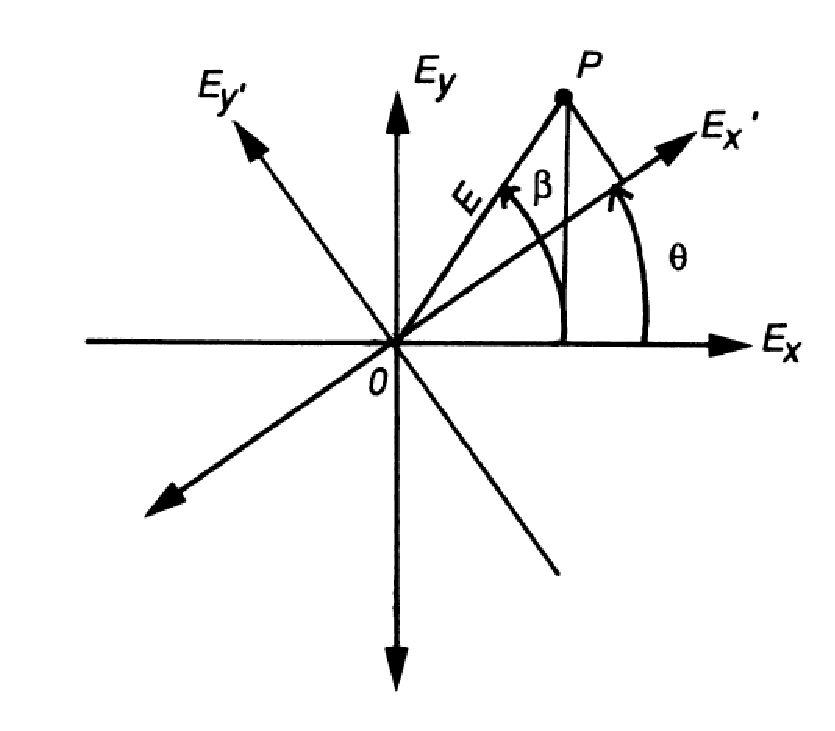
\includegraphics[width = 0.35\textwidth]{Chapter4/Figures/rotator.eps}
 \caption{Rotation of the opticalto Polarization field components by rotator}
 \label{fig:rotator}
\end{figure}
%\vspace{-1cm}

\begin{equation}
	\label{Eq:Rot}
\small
	E'_{x} = E_{x}\cos\theta + E_{y}\sin\theta \hspace{1 cm}
	E'_{y} = -E_{x}\sin\theta + E_{y}\cos\theta~. 
\end{equation}

\begin{equation}
\label{Eq:GenRotMul}
\small
	M(2\theta)= 
	\begin{bmatrix}
	1   & & 0  & & 0  & &0\\ 0   & &\cos 2\theta  & &\sin 2\theta  & &0\\0  & & -\sin 2\theta   & & \cos 2\theta  & & 0\\0  & &0  & & 0  & & 1\\
	\end{bmatrix}~.
\end{equation}

\end{description}
 

The polarizer and retarder are often rotated while being used in optics.
For this reason, it is useful to mention the Mueller matrix of the rotated polarizer and rotated retarder.
First, assume the polarizer is rotated at the same time.
The incident beam first goes through the rotator with the Mueller matrix of $M_{R}(2\theta)$, and then through the polarizer with the Mueller matrix ($M$).
In this case, the emerging Stokes vector in terms of original axis is given by \ref{Eq:rotpol}.
Eq.~\ref{Eq:RotPolMul} represents the Mueller matrix of the rotated polarizer.
%which is the result of multiplying inverse rotation Mueller matrix, the angular form of polarizer Mueller matrix and rotation Mueller matrix. 
\begin{equation}\label{Eq:rotpol}
\small
	S' = M_{R}(-2\theta)MM_{R}(2\theta)~.
\end{equation}

\begin{equation}\label{Eq:RotPolMul}
\small
	M = \frac{p^{2}}{2} 
	\begin{bmatrix}
	 1  & & \cos 2\gamma\cos 2\theta  & & \cos 2\gamma \sin 2\theta  & & 0\\ 
	 \cos 2\gamma\cos 2\theta   & & \cos^{2} 2\theta + \sin 2\gamma \sin^{2} 2\theta  & & (1-\sin 2\gamma)\sin 2\theta \cos 2\theta  & &  0\\
	 \cos 2\gamma \sin 2\theta   & & (1-\sin 2\gamma)\sin 2\theta \cos 2\theta  & & \sin^{2} 2\theta + \sin 2\gamma \cos^{2} 2\theta  & & 0\\
	 0  & & 0  & & 0  & & \sin 2\gamma\\
	\end{bmatrix}~,   
\end{equation}

\noindent The matrix represented in Eq.~\ref{Eq:RotPolMul} is the general form.
Thus, for different values of $\gamma = 0^{\circ} , 45^{\circ}$ and $90^{\circ}$, the matrix represent the linear horizontal polarizer, the neutral density filter and the linear vertical polarizer, respectively.
The Mueller matrix of an ideal linear horizontal polarizer is shown in Eq.~\ref{Eq:HRotPolMul}. 
\begin{equation}\label{Eq:HRotPolMul}
\small
	M = \frac{1}{2} 
	\begin{bmatrix}
	 1  & & \cos 2\theta  & & \sin 2\theta  & & 0\\ 
	 \cos 2\theta   & & \cos^{2} 2\theta  & & \sin 2\theta \cos 2\theta  & & 0\\
	  \sin 2\theta   & & \sin 2\theta \cos 2\theta  & & \sin^{2} 2\theta   & & 0\\
	 0  & &0  & &0  & &0\\
	\end{bmatrix}~.
\end{equation}
%Table \ref{Tab:Chp4T3} represents the Mueller matrices for horizontal, vertical and $\pm 45^{\circ}$ linear and circular polarizers. 
%\input{Chapter4/Table3.tex}

\noindent The Mueller matrix of a rotated retarder is calculated in the same manner.
Equation.~\ref{Eq:RotRetMul} represents the general form of rotated retarder Mueller matrix. 
\begin{equation}\label{Eq:RotRetMul}
\small
	M(\phi , 2\theta)= 
	\begin{bmatrix}
	 1  & & 0  & & 0  & & 0\\ 
	 0  & &\cos^{2} 2\theta + \cos \phi \sin^{2} 2\theta  & & (1-\cos \phi)\sin 2\theta \cos 2\theta  & &   -\sin \phi \cos 2\theta\\
	 0  & & (1-\cos\phi)\sin 2\theta \cos 2\theta  & & \sin^{2} 2\theta + \sin \phi \cos^{2} 2\theta  & & \sin \phi \cos 2\theta\\
	 0  & & \sin \phi \sin 2\theta  & & -\sin \phi \cos 2\theta  & &\cos \phi\\
	\end{bmatrix}~.
\end{equation}




%A medium can possesses similar properties than optical elements to change the polarization states of the incident light.
%A medium can contain depolarization, birefringence (retardants) and diattenuation properties. 

%	\begin{description}
%	\item[Depolarization] - If an initial state of the light is 100$\%$ polarized and polarization degree of the existing state is less than unity, the system posses the depolarization property. Depolarization is usually encountered due to multiple scattering of photons.
%	The general form of a pure depolarization Mueller matrix is shown in Eq.\ref{Eq:DepolarizationMul}.
%	Here $1-\vert a \vert$ and $1-\vert b \vert$ are depolarization factors for linear polarization states and $1-\vert c \vert$ represents depolarization factor for circular polarization. The net depolarization factor is shown in Eq. \ref{Eq:netDepolarizationfac}
%	\begin{equation}\label{Eq:DepolarizationMul}
%	\small
%		M_{\Delta} = \begin{bmatrix}
%	1 & & 0 & & 0 & & 0\\0 && a && 0 && 0\\ 0 && 0 && b && 0\\ 0 && 0 && 0 && c
%	\end{bmatrix} , \hspace{1 cm} \vert a \vert, \vert b \vert, \vert c \vert \leq 1
%	\end{equation}
%	\begin{equation}\label{Eq:netDepolarizationfac}
%	\small
%		\Delta  = 1 - \frac{\vert a \vert + \vert b \vert + \vert c \vert }{3} = 1 - \frac{\vert tr (M_{\Delta}-1)\vert}{3} , \hspace{0.5 cm} 0\leq \Delta \leq 1
%		\end{equation}		
%	\item[Retardance] - is the phase shift between orthogonal components of polarized light and it occurs due to differences in refractive indices of different polarized states. 
%	
%	Birefringence is a linear retardants which occurs due to phase difference between orthogonal linear polarization states (between vertical and horizontal or between $45^{\circ}$ and $-45^{\circ}$ ).
%	Mueller matrix of linear retardance ($\delta$) while its fast axis is rotated by angle $\theta$ with respect to the horizontal axis is shown in Eq.\ref{Eq:Birefringence}
%	\begin{equation}\label{Eq:Birefringence}
%	\small
%	M_{R_{B}}=\begin{bmatrix}
%	1 &&  0 &&  0  && 0\\
%	0 && \cos^{2}2\theta +\sin^{2}2\theta\cos\delta && \sin 2\theta\cos 2\theta(1-\cos\delta) &&  -\sin 2\theta \sin \delta\\ 
%	0 &&\sin 2\theta\cos 2\theta(1-\cos\delta) && \sin^{2}2\theta +\cos^{2}2\theta\cos\delta && \cos 2\theta \sin \delta\\
%	 0 && \sin 2\theta \sin \delta && -\cos 2\theta \sin \delta && \cos\delta
%	\end{bmatrix}
%	\end{equation}	

%	Beside linear retardance, there is circular retardance $\psi$ (optical rotation) as well, which arises due to phase difference between right circularly polarized (RCP) and left circularly polarized (LCP) states. 
%	The Mueller matrix for a circular retardance is shown in Eq.\ref{Eq:CircularRet}.
%	\begin{equation}\label{Eq:CircularRet}
%	\small
%	M_{R_{C}}=\begin{bmatrix}
%	1 &&  0 &&  0  && 0\\
%	0 && \cos 2\psi && -\sin 2\psi &&  0\\ 
%	0 && \sin 2\psi && \cos 2\psi && 0\\
%	 0 && 0 && 0 && 1
%	\end{bmatrix}
%	\end{equation}
%	
%	\item[Diattenuation ($d$)] - of an optical elements corresponds to differential attenuation (absorption and scattering) of orthogonal polarizations for both linear and circular polarizations states.
%	Accordingly linear diattenuation is defined as differential attenuation of two orthogonal linear polarization states and circular diattenuation is defined as differential attenuation of RCP and LCP.
%	Mueller matrix of linear diattenuator is defined in Eq.\ref{Eq:LinearDiattenuation}. 
%	Here two intensity transmittance (reflectance) parameters ($q$, $r$) are used for orthogonal states and $\theta$ is the orientation angle of principal axis. 
%	
%	\begin{equation}\label{Eq:LinearDiattenuation}
%	\small
%	M_{D}=\begin{bmatrix}
%	q+r &&  (q-r)\cos 2\theta &&  (q-r)\sin 2\theta && 0\\
%	(q-r)\cos 2\theta && (q+r)\cos^{2}2\theta + 2\sqrt{(qr)}\sin^{2}2\theta && (q+r-2\sqrt{(qr)})\sin 2\theta\cos 2\theta & & 0\\ 
%	(q-r)\sin 2\theta && (q+r-2\sqrt{(qr)})\sin 2\theta\cos 2\theta && (q+r)\cos^{2}2\theta + 2\sqrt{(qr)}\sin^{2}2\theta && 0\\
%	 0 && 0 && 0 && 2\sqrt{(qr)}
%	\end{bmatrix}
%	\end{equation}		
%	\end{description}

A medium (tissue) can possess different optical properties at the same time.
In order to obtain these properties, inverse polarimetry based on Mueller matrix decomposition is used.
The Lu-Chipman decomposition method \cite{lu1996interpretation} is a well known inverse polarimetry analysis explained in the following.

%{\color{red}
%you can mention that there is technics than can estimates or measure the Mueller matrix of a medium and then it is sometimes useful to decompose the measured matrix in order to deduce the physical properties of the medium.}

					

%Inverse polarimertry based on Mueller matrix decomposition is used to obtain the optical properties of the tissue.
%The mentioned optical properties of the tissue can be calculated using inverse polarimetry analysis based on Mueller matrix decomposition.
%The Lu-Chipman decomposition method \cite{lu1996interpretation} is a well known inverse polarimetry analysis which is explained in the following.

\subsection{The Lu-Chipman decomposition}
The proposed method of Lu-Chipman \cite{lu1996interpretation} allows a Mueller matrix to be decomposed into the product of three matrices of diattenuation, depolarization and retardant (See Eq.\ref{Eq:LuchimpanDec}).
In this representation, $M_{\Delta}$ describes the depolarizing effects of the medium, $M_{R}$ shows the effects of linear birefringence and $M_{D}$ includes the effect of linear and circular diattenuation. 

 	\begin{equation}\label{Eq:LuchimpanDec}
	\small
	M\Leftarrow M_{\Delta}.M_{R}.M_{D}~.\\
	\end{equation}
	
	
	\begin{align}
	M_{\Delta} = 
	\begin{bmatrix}
	1 &  \overrightarrow{0}\\ \overrightarrow{P_{\Delta}}  & m_{\Delta}
	\end{bmatrix} \qquad
	M_{R} = 
	\begin{bmatrix}
	1 & \overrightarrow{0}\\ 0 & m_{R}
	\end{bmatrix} \qquad \
	M_{D} = 
	\begin{bmatrix}
	1 & \overrightarrow{D}^{T}\\ \overrightarrow{D} &  m_{D} \
	\end{bmatrix}~.
	\end{align}
\noindent Each of these matrices can be calculated and further used to extract individual medium properties such as the \textit{diattenuation} factor $D$, \textit{depolarization} $\Delta$, \textit{linear retardance} $\delta$, and a circular retardance $\psi$. Calculation of these parameters are explained step by step in the following. 

Starting with diattenuation, the $3 \times 3$ sub-matrix $m_{D}$ is defined by: 

	\begin{equation}\label{eq:Diatt}
	\small
     m_{D}  = \sqrt{1-D^{2}}I  + \frac{1 - \sqrt{1-D^{2}}}{D^{2}} \overrightarrow{D} \overrightarrow{D}^{T}~,
	\end{equation}
\noindent where $I$ is the $3 \times 3$ unity matrix, $\overrightarrow{D}$ is the diattenuation vector and $D$ is the diattenuation value $D = \vert \overrightarrow{D} \vert$. 
\begin{align}\label{eq:diattenuationvec}
\overrightarrow{D} & = \frac{1}{m_{11}} [m_{12}\quad m_{13} \quad m_{14}]^{T}~,\\
D & = \frac{1}{m_{11}} \sqrt{m_{12}^{2} + m_{13}^{2} + m_{14}^{2}}~.
\end{align}
Using the diattenuation matrix, the depolarization matrix can be computed.
	\begin{equation}\label{eq:reformLCD}
	\small
	M_{\Delta}M_{R} = M' = M M_{D}^{-1} =
	\begin{bmatrix}
	1 & \overrightarrow{0}\\
	\overrightarrow{P_{\Delta}} & m'
	\end{bmatrix}~,
	\end{equation}
\noindent In this matrix, $\overrightarrow{P}_{\Delta}$ is based on  the polarizance vector $\overrightarrow{P}$ and the sub-matrix $m$ of the Mueller matrix $M$, (See Eq.\ref{eq:polarizance}) 	
	\begin{subequations}\label{eq:polarizance}
	\small
	\begin{align}	
	\overrightarrow{P} = \frac{1}{m_{11}}[m_{21} \quad m_{31} \quad m_{41} ]^{T}~,\\
	\overrightarrow{P_{\Delta}} = \frac{(\overrightarrow{P} - m \overrightarrow{D})}{1-D^{2}}~,
	\end{align}
	\end{subequations}
	
\noindent $m' = m_{\Delta}m_{R}$.
Since $m_{\Delta}$ is a symmetric matrix, its eigenvalues define its depolarization properties, $m_{\Delta}^{T} = m_{\Delta}$ and $m_{\Delta}^{2} = m'(m')^{T}$. Thus $m_{\Delta}$ can be represented in terms of eigenvalues of $m'(m')^{T}$.
\begin{align*}
\small 
m_{\Delta} & = \pm[m'(m')^{T} + (\sqrt{\lambda_{1}\lambda_{2}} + \sqrt{\lambda_{2}\lambda_{3}} + \sqrt{\lambda_{3}\lambda_{1}})I]^{-1} \\
& \times [(\sqrt{\lambda_{1}} +\sqrt{\lambda_{2}} + \sqrt{\lambda_{3}})m'(m')^{T} + \sqrt{\lambda_{1}\lambda_{2}\lambda_{3}} I]~.
\end{align*}

\noindent Once the depolarization matrix $m_{\Delta}$ is obtained, the sub-matrix of retardance is processed by $m_{R} = m_{\Delta}^{-1} m'$.
Following the sub-matrices obtained, the depolarization power and total retardance is calculated by: 
\begin{align}
\Delta & = 1 - \frac{\vert tr(m_{\Delta}) \vert}{3}~,\\
R  & = \cos^{-1} \left[ \frac{tr(M_{R})}{2} - 1\right]~.
\end{align}

%The last factor is retardant matrix $M_{R}$. which can be reformed as follows (See Eq.\ref{eq:MR}). In this representation $m_{R}$ is the sub-matrix of $M_{R}$ and is computed using polarizance and diattenuation factors and sub-matrix of $M$ as it is presented in Eq.\ref{eq:subMR}
%	\begin{equation}\label{eq:MR}
%	\small
%	M_{R} = \begin{bmatrix}
%	1 && \overrightarrow{0}^{T}\\
%	\overrightarrow{0} && m_{R}
%	\end{bmatrix}	
%	\end{equation}		
%	
%	\begin{equation}\label{eq:subMR}
%	\small
%	m_{R} = \frac{1}{\sqrt{(1-d^{2})}}[m - \frac{1-\sqrt{1-d^{2}}}{d^{2}}(\overrightarrow{P}.\overrightarrow{d}^{T})]
%	\end{equation}
%	
%The combined effects of linear and circular retardance is computed by Eq.\ref{eq:TR}. 
%	\begin{equation}\label{eq:TR}
%	\small
%	R = \cos^{-1}\lbrace{\frac{Tr(M_{R})}{2}-1 \rbrace}
%	\end{equation}

Using this method, the individual parameters of the medium can be computed.
Table~\ref{Tab:ParMed} summarizes these parameters, conditioned to having retardance, depolarization and diattenuation Mueller matrices.
In this table, $M(i,j)$ represents the element in the $i^{th}$ row and the $j^{th}$ column of the matrix. 

	\begin{table}
	\small
	\begin{center}
	\caption{Medium Characteristics}
	\begin{tabular}{|c|c|c|}
	\hline
	Parameters & Notations & Equation \\
	\hline 
	& & \\
	 Linear retardance & $\delta$ & $ \cos^{-1}(\sqrt{[M_{R}(2,2)+ M_{R}(3,3)]^{2} +[M_{R}(3,2)+ M_{R}(2,3)]^{2}}-1)$\\
	 & & \\
	Optical rotation & $\psi$ & $\tan^{-1}[(M_{R}(3,2)-M_{R}(2,3))(M_{R}(2,2)-M_{R}(3,3))^{-1}]$\\
	& & \\
	Diattenuation & $D$ & $M_{D}(1,1)^{-1}\sqrt{M_{D}(1,2)^{2}+M_{D}(1,3)^{2}+M_{D}(1,4)^{2}}$\\
	& & \\
	Depolarization & $\Delta$ & $1 - \frac{\vert Tr (M_{\Delta}-1)\vert}{3}$\\
	& & \\
	\hline   
  	\end{tabular}
  	\label{Tab:ParMed}
  	\end{center}
	\end{table}

%Since matrix multiplication is generally non commutative, one should concerns about the multiplication order of Lu-Chipman matrices and the effects displacement. The influence of these orders were investigated by \cite{ghosh2010influence}. Their results indicated that for the turbid media with weak diattenuation, the extracted polarization parameters are independent of the selected multiplication orders. These results were confirmed for biological tissues due to their weak diattenuation effects. Therefore it was concluded that individual tissue polarimetry effects can be successfully quantified despite their simultaneous occurrence, even in the presence of numerous complexities due to multiple scattering \cite{ghosh2010influence}.






\section{Image Polarimetry in Biomedical Field} \label{sec:chp4-sec5}
Image polarimetry refers to different approaches to describe the propagation of polarized light, its interactions with the optical system, and its medium polarized properties.
The Stokes and Mueller systems are well suited for polarimetry applications, since first they can document the full, partial and un-polarized state of light and second they provide an intensity measure and experimental data.

The Stokes and Mueller polarimetries refer to measuring the Stokes vector and the Mueller matrix, respectively.
These systems can be used either to highlight the different layers of the tissue by showing diffuse light coming from deeper layers and showing the medium response with different polarized conditions (Stokes polarimetry) or to highlight some medium characteristics (Mueller polarimetry).

Although the polarization filters are employed in a \acf{pd} in order to remove any specular reflection of light and capture the backscattered light from deeper levels of the skin, the full potential of image polarimetry in biomedicine has not been explored~\cite{ghosh2011tissue}.
%Gosh~et al.\,\cite{ghosh2011tissue} summarizes 
%Presumably this is due to the challenges such as~\cite{ghosh2011tissue}: 
%	\begin{itemize}
%	\item Extensive loss of polarization signal as a effect of tissue multiple scattering 
%	\item Complicated nature of polarization effects in tissue
%	\item Measurements difficulty, specially for small polarization signals
%	\item Challenges in analysis and quantification of measured signals or images 
%	\item Complexities in understanding and analyzing the obtained results 
%	\item Lack of detailed information on polarimetric properties of various tissues and their effects on polarized propagation.
%	\end{itemize}
	
Currently, several researchers are pursuing innovative solutions in the filed of image polarimetry.
A comprehensive summary of current research in polarimetry and it's problems is provided by Ghosh~et al.\,\cite{ghosh2011tissue}.
%Ghosh~et al.\,\cite{ghosh2011tissue} provided a good summary on the current stage of the research in polarimtery and its problems.
Polarimetry systems can be used either for tissue imaging or analyzing the tissue's optical characteristics.
We categorized the applied polarimetry systems into three groups: (i) partial Stokes polarimeters, (ii) Stokes polarimeters, and (iii) Mueller polarimeters.
The techniques in the first two categories are used to define the polarization state of the backscattered light from the object and the last one is used to detect the optical properties of the sample.
The aforementioned groups and their related studies are discussed in the following.


%However the Stokes-Mueller polarimetry is more suited for polarimetry applications due to two reasons. First the polarized light after interaction with the medium could be fully, partial or un-polarized and Jones calculus is only applicable for fully polarized light state.
%Second intensity measurements of polarized lights and experimental data are more desirable and Mueller formalism is based on experimental consideration of intensity measurements.
%Based on mentioned reasons, the Stokes-Mueller polarimetry is explained in the following. 
% Stokes-Mueller polarimetry system contains two major elements; \textit{PSA}, polarization states analyser and \textit{PSG}, polarization states generator. The \textit{PSA} contains a set of elements which analyse the polarization state of incoming light and \textit{PSG} contains the elements which generate the polarization states. Three main subcategory of polarimetry are introduced by \cite{goldstein2003polarized}, which includes:
%\begin{itemize}
%	\item Rotating element polarimetry \\
%	The Stokes vector and Mueller matrix parameters are measured here with rotating the polarized elements (polarizer, retarder). 	
%	\item Oscillating element polarimetry \\
%	Which rotates the polarization of light using some electro or magneto-optical device such as liquid crystal cell. 
%	\item Phase modulation polarimetry \\
%	These polarimeters use devices that vary in retardance in response to an electrical signal.
%\end{itemize} 
%
%However different types of imaging polarimetry systems had implemented in the literature which does not follow the mentioned category exactly. These systems are discussed with their details in section \ref{polState}.
%\input{Chapter4/ImagePolarimetry-LuChip.tex}

%\subsection{Polarimetry Systems in Biomedical field}
%\label{polState}
\subsection{Partial Stokes polarimeters}
Beside the conventional use of cross-polarized filters in dermoscopes, the polarization and polarimetry systems have been used by several researchers as imaging techniques.
This section describes the image polarimeters which were built to create the first two or three Stokes parameters.
	
Jacques et al \cite{Jacques12175282} were among the first researchers to consider analysing polarized images rather than single image for skin imaging.
In their research they proposed the use of two polarized filters.
A polarizer generator was placed in the incident path in order to create the linearly polarized light illumination and polarizer analyser in the detection path.
In this system the angle of the incident was chosen in a way that only backscattered light was collected with the camera.
The authors proposed two image acquisitions: one with the analysing polarizer oriented parallel to the illumination and one with the analyser positioned perpendicular to the illumination.
%The algebraic combination of these images ($I_{pol} = \frac{I_{par}-I_{per}}{I_{par}+I_{per}}$) leads to an image that emphasizes on the superficial skin structures which scattered the light rather than structures that absorb light \cite{Jacques12175282}.
The algebraic combination of these images ($I_{pol} = \frac{I_{\parallel}-I_{\perp}}{I_{\parallel}+I_{\perp}}$) leads to an image (depolarization ratio image) which is sensitive to superficially scattered polarized light and visualizes the disruption of the normal texture of the papillary and upper reticular dermis by skin pathology~\cite{Jacques12175282}. 
The authors used these imaging techniques for the differentiation of clinical images of skin pathologies. 
%The combination of co and cross polarized images $I_{pol}$ in addition to multispectral set up was used by \cite{yaroslavsky2003} as well. This set up was used for detection the boundaries of non melanoma parts with in the lesion. 

Another project based on the first two Stokes parameters was proposed by Anastasiadou~et al.\,\cite{Anastasiadou2008}.
In this work the authors proposed polarimetric imaging for imaging cervical cancers.
Figure.~\ref{fig:SPcervicalcancer} illustrates their proposed systems.
\begin{figure}[h]
\centering
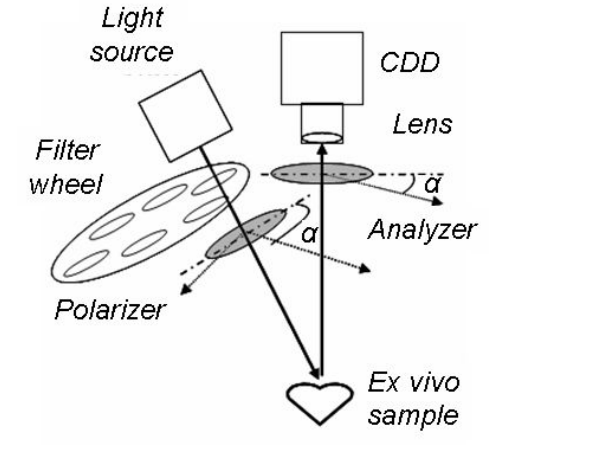
\includegraphics[width = 0.5\textwidth]{Chapter4/Figures/ImagePolarimetryCervicalCancer.png}
\caption[Polarimetry system proposed by \cite{Anastasiadou2008}]{Polarimetric image system proposed by \cite{Anastasiadou2008}.}
\label{fig:SPcervicalcancer}
\end{figure}
\noindent In this figure, $\alpha$ is the azimuth angle and the two images are acquired, $I_{\parallel}$ when the the two polarizers are positioned parallel to each other and $I_{\perp}$ when they are perpendicular.
The proposed system consists of a white light source (150 W halogen bulb), a fiber handle, a filter wheel (three channels 450, 550, and 650 \si{\nano\meter}), a linear polarizer/ analyzer, and finally a CCD camera~\cite{Anastasiadou2008}.
Using this setup, similar to the previous study, the $I_{pol}$ image is calculated as a final image (referred to as $DOP$ in the study).
A classification framework of ex-vivo cervical lesions (76 patients) using the images provided by the proposed imaging system, achieved a \ac{se} of 52-86\% and \ac{sp} of 93\%.
%Examination of the the proposed imaging system on ex-vivo cervical lesions, 76 patients, achieved a \ac{se} of 52-86\% and \ac{sp} of 93\%.
Figure.~\ref{fig:CC-Ex1} illustrates a sample of severe dysplasia comparing images seen under colposcopy and the proposed polarimetry system.
\begin{figure}[h]
\begin{center}
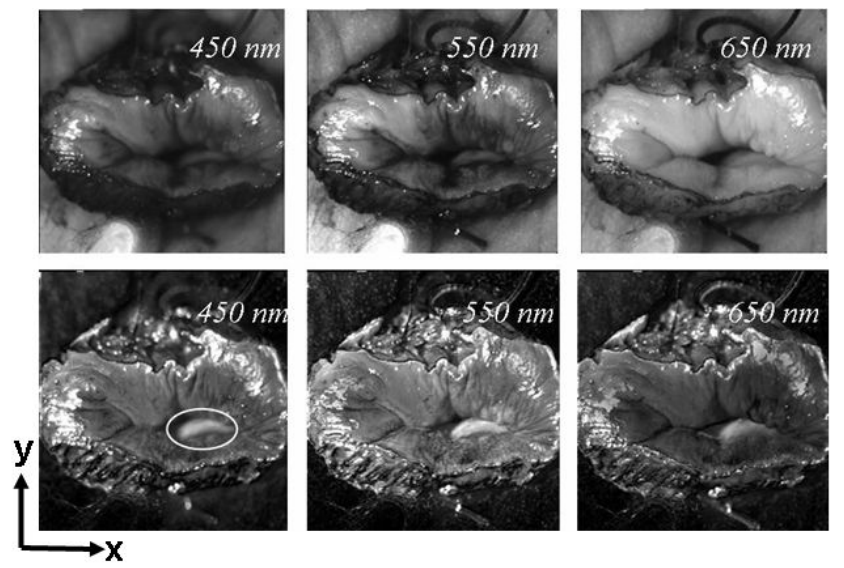
\includegraphics[width = 0.7\textwidth]{Chapter4/Figures/CC-Ex1.png}
\caption[Polarimetry images of ex-vivo cervical dysplasia~\cite{Anastasiadou2008}]{$I_{\parallel}$ and $I_{pol}$, first and second row, respectively. The images were taken with $\alpha = 0$ and at different wavelengths. Images presented by \cite{Anastasiadou2008}.}
\label{fig:CC-Ex1}
\end{center}
\end{figure}
This example was presented as a case, in which the confirmed dysplasia region was not obvious in ordinary images.
However it was clearly noted in the $I_{pol}$ image.

Zhao~et al.\,\cite{zhao2009} introduced another partial polarimetry (spectropolarimetric) imaging system to measure pathological changes of tissue birefringence and structure. 
Figure.~\ref{fig:Zhaosys} shows the proposed system by \cite{zhao2009}.
		\begin{figure}
		\centering
		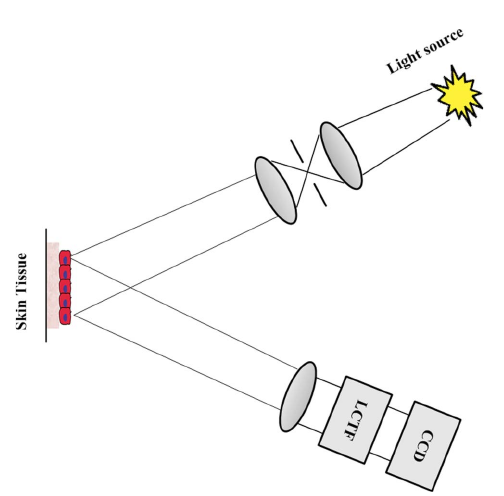
\includegraphics[width = 0.5\textwidth]{Chapter4/Figures/spectropolarimeter.png}	
	\caption[Polarimetry system proposed by \cite{zhao2009}]{The polarimetry system developed by \cite{zhao2009}.}
		\label{fig:Zhaosys}
		\end{figure}	
\noindent This system is composed of an incoherent white light source (halogen) illuminated in a collimated beam at an angle of \ang{25} to the normal of the skin surface and a CCD camera along with a \ac{lctf} used to acquire spectropolarimetric images.
The \ac{lctf} is a bandpass filter that can control the wavelength of the transmitting light and ranges from 400-720\si{\nano\meter}.
The spectropolarimetric images are acquired by manually rotating the \ac{lctf} at \ang{0}, \ang{45}, \ang{90}, and \ang{135} angles.
Using the acquired images the three first Stokes parameters as well as the \ac{dolp} were measured (see Eq.\,\ref{Eq:DP} and Eq.\,\ref{Eq:cStokesmeas}). 
Figure.~\ref{fig:Zhao-ex1} shows an example of the Stokes parameters and \ac{dolp} obtained for chilblain skin at 590 \si{\nano\meter}.
\begin{figure}[t]
\begin{center}
\subfloat[$S_{0}$]{
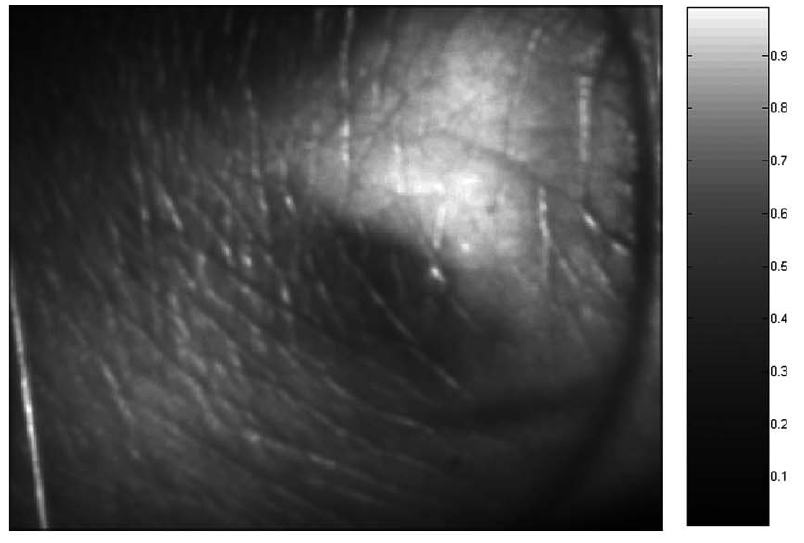
\includegraphics[width = 0.44\textwidth]{Chapter4/Figures/Zhao-ex1-a.png}}\
\subfloat[$S_{1}$]{
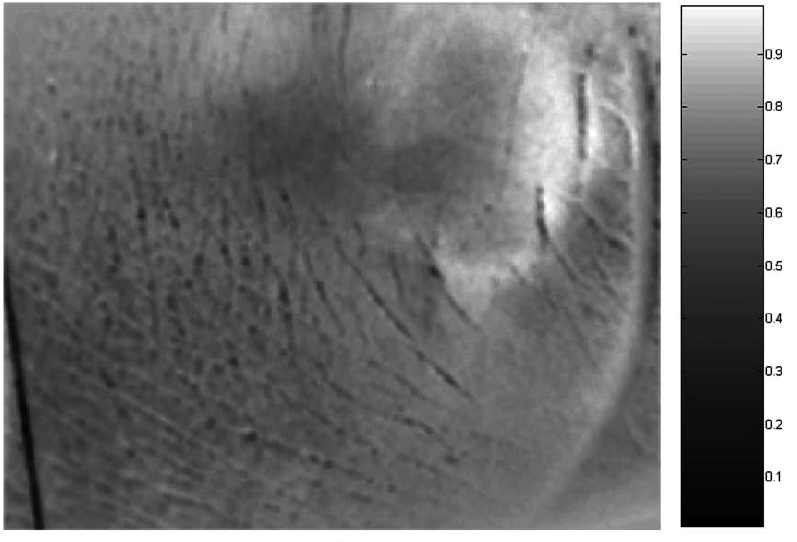
\includegraphics[width = 0.44\textwidth]{Chapter4/Figures/Zhao-ex1-b.png}}\\
\subfloat[$S_{2}$]{
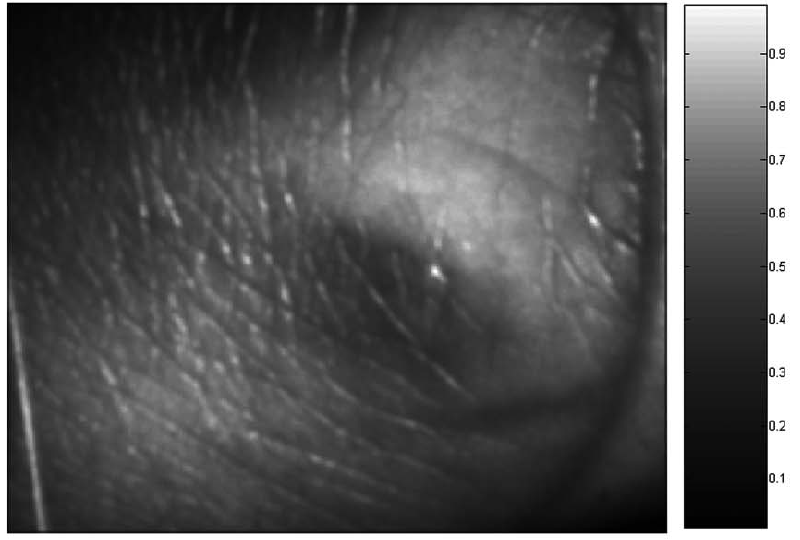
\includegraphics[width = 0.44\textwidth]{Chapter4/Figures/Zhao-ex1-c.png}}\
\subfloat[\ac{dolp}]{
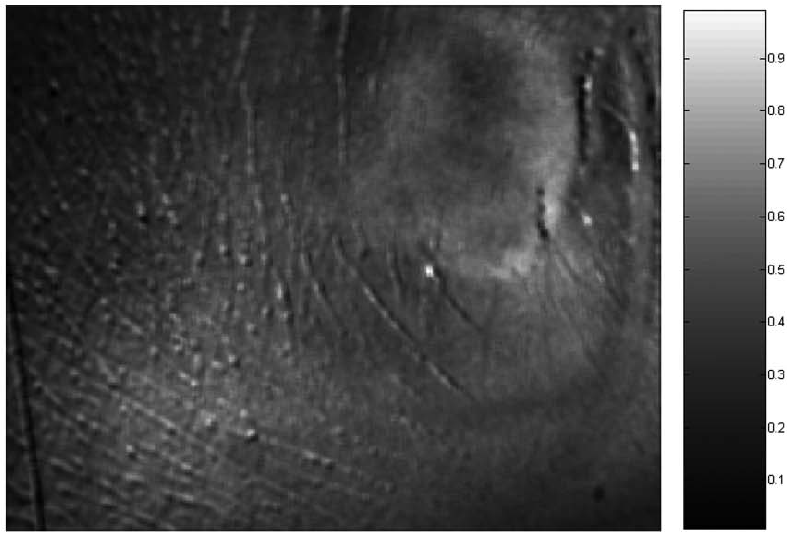
\includegraphics[width = 0.44\textwidth]{Chapter4/Figures/Zhao-ex1-d.png}}
\caption[Polarimetry images of Chilblain skin sample~\cite{zhao2009}]{Chilblain skin sample described by the first three Stokes parameters and \ac{dolp}. Images presented by \cite{zhao2009}.}
\label{fig:Zhao-ex1}
\end{center}
\end{figure} 

Recently, Tchvialeva~et al.\,\cite{tchvialeva2013polarization} proposed using polarization speckle patterns to differentiate and identify skin cancer lesions.
In this research the author proposed calculating the depolarization ratio ($I_{pol}$) from the backscattered speckle patterns using the proposed system shown in Fig.~\ref{fig:TchialevaSys}.
This system is composed of dual cameras, two diode lasers: a blue laser ($\lambda = 407$~\si{\nano\meter}) and a red laser ($\lambda = 663$~\si{\nano\meter}), a diaphragm and a beam splitter.
The speckle patterns are recorded simultaneously by both cameras, one captures the light parallel to the initial polarization and the other captures the light perpendicular to the initial polarization~\cite{tchvialeva2013polarization}.
Figure.~\ref{fig:tchvialeva-ex1} shows examples of polarization speckle patterns for a malignant melanoma, a squamous cell carcinoma, a basal cell carcinoma, a nevus, and a seborrheic keratosis using the blue laser. 
\begin{figure}[tb]
\begin{center}
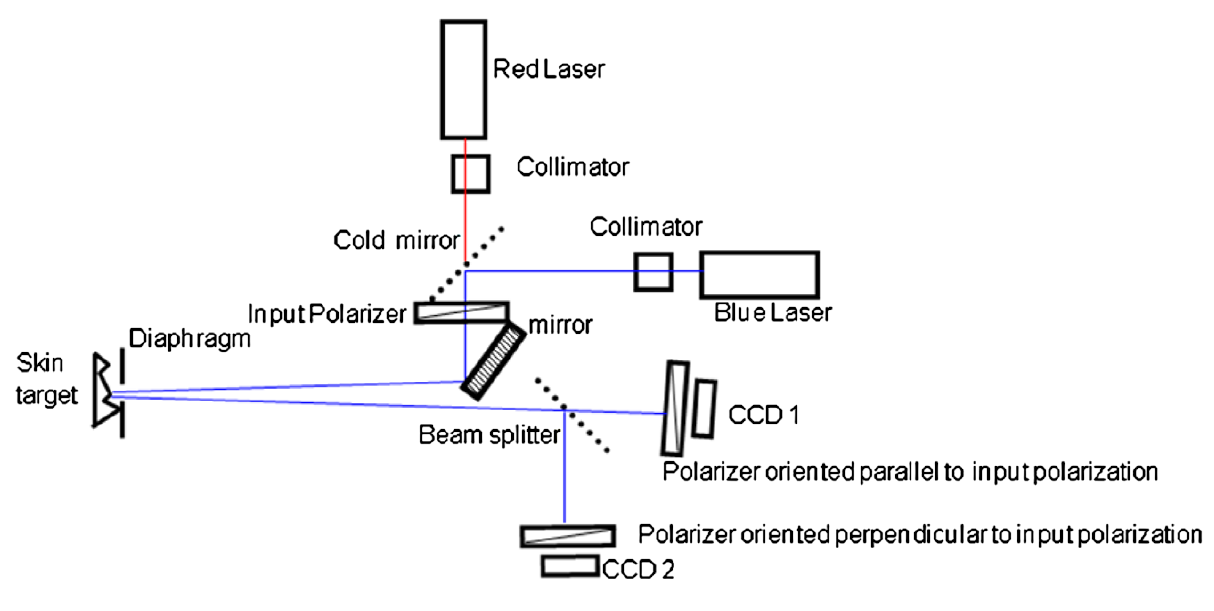
\includegraphics[width= 0.85\textwidth]{Chapter4/Figures/TchvialevaSys.png}
\caption[Polarimetry system proposed by \cite{tchvialeva2013polarization}]{The laser speckle device proposed by \cite{tchvialeva2013polarization}.}
\label{fig:TchialevaSys}
\end{center}
\end{figure}
\begin{figure}
\begin{center}
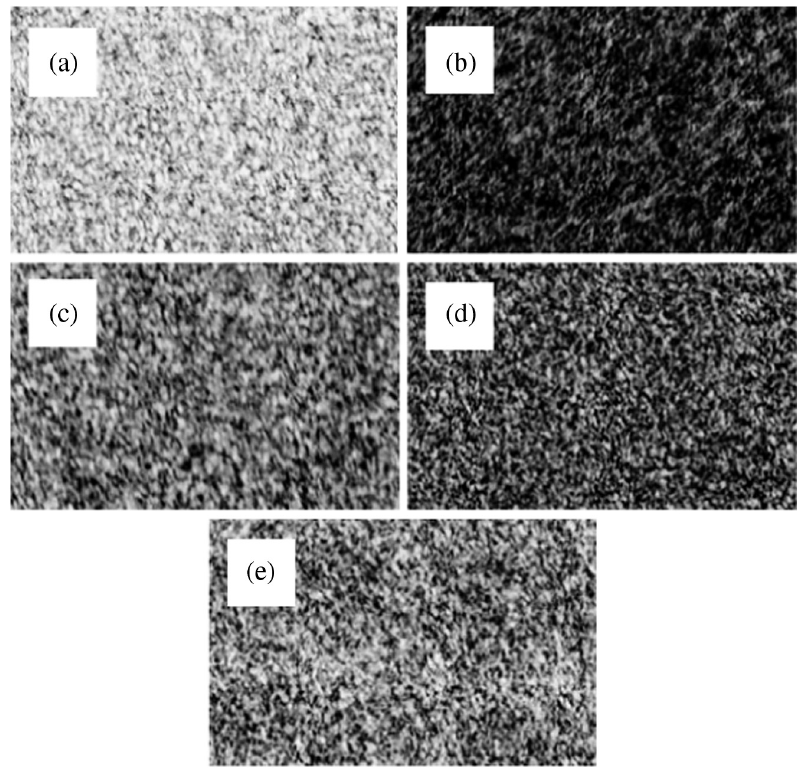
\includegraphics[width = 0.7\textwidth]{Chapter4/Figures/Tchvialeva-ex1.png}
\caption[Speckle polarimetry images of skin lesions]{Examples of polarization speckle patterns of skin lesions using a blue laser (407~\si{\nano\meter}); (a) A malignant melanoma, (b) A squamous cell carcinoma, (c) A basal cell carcinoma, (d) A nevus, and (e) seborrheic keratosis. Images are taken from \cite{tchvialeva2013polarization}.}
\label{fig:tchvialeva-ex1}
\end{center}
\end{figure}
\noindent The authors evaluated their proposed systems on in-vivo 214 skin lesions containing cancer and benign lesions where they reported that statistical moments of the polarization speckle pattern is able to separate malignant melanoma from sebrroheic keratosis, basal cell carcinoma, and squamous cell carcinoma.

	

\subsection{Stokes polarimeters}
A classical approach for measuring the four Stokes parameters was mentioned in Sect.~\ref{sec:chp4-sec3} (see Eq.~\ref{Eq:cStokesmeas}). 
As discussed in the previous section, this approach was partially used in several studies to measure the two or three first Stokes parameters~\cite{tchvialeva2013polarization,zhao2009,Jacques12175282,Anastasiadou2008}.
The choice of partial measurements using the aforementioned setup is because measuring the fourth parameter ($S_{3}$) is relatively more difficult and less accurate than the first three parameters.
This is due to reasons such as: (i) the optical energy absorbed by the retarder should be accounted for when measuring $S_{3}$, (ii) the retarder should be removed and replaced during the acquisition, and  (iii) the perfect alignment of the transmission axis of the polarizer at \ang{45} from the fast axis of the retarder is required.
These factors have made it difficult to accurately measure the $S_{3}$ parameter, using this setup.
To address this problem, Collett\,\cite{collett1984measurement} proposed to use one optical element instead of two.
Collett proposed using a circular polarizer constrcuted by a linear polarizer whose transmission axis is rotated at \ang{45} with respect to the horizontal axis followed by a quarter-wave retarder which its fast axis is parallel to the horizontal direction. 
Using this setup, the three intensities ($I_{C}(\theta)$) are measured when the circular polarizer is rotated at \ang{0}, \ang{45}, and \ang{90} with respect to the horizontal axis and the fourth intensity ($I_{L}(\theta)$) is measured by flipping the linear polarizer to the other side (i.e. the linear polarizer follows the quarter retarder) and keeping its axis parallel to the horizontal axis (i.e. $\theta = \ang{0}$)~\cite{collett1984measurement,ghosh2011tissue}.
The Stokes parameters are calculated from the four measured intensities using the following equation:
\begin{equation}\label{eq:CollettStokes}
\begin{bmatrix}
S_{0} \\ S_{1} \\ S_{2} \\ S_{3} 
\end{bmatrix} = 
\begin{bmatrix}
I_{C}(\ang{0}) + I_{C}(\ang{90}) \\
S_{0} - 2I_{C}(\ang{45}) \\
I_{C}(\ang{0}) - I_{C}(\ang{90})\\
-S_{0} +2I_{L}(\ang{0})
\end{bmatrix}~.
\end{equation}
\noindent This method was used in several researches to measure the Stokes parameters of the light or backscattered light from the tissue~\cite{sankaran1999polarization, ghosh2004depolarization}.

Although this method is more accurate than the classical approach, in order to improve the sensitivity of the measurement it was proposed to use polarization modulation with synchronized detection.
Although such systems provide signals rather than images, they have been used in several studies to measure sample polarization properties~\cite{sankaran2002comparative,wood2008towards}. 
The system proposed by Wood~et al.\,\cite{wood2008towards}, using polarization modulation and a synchronous lock-in-amplifier is shown in Fig.~\ref{fig:pmodulationStokes}.
	\begin{figure}
	\centering 
	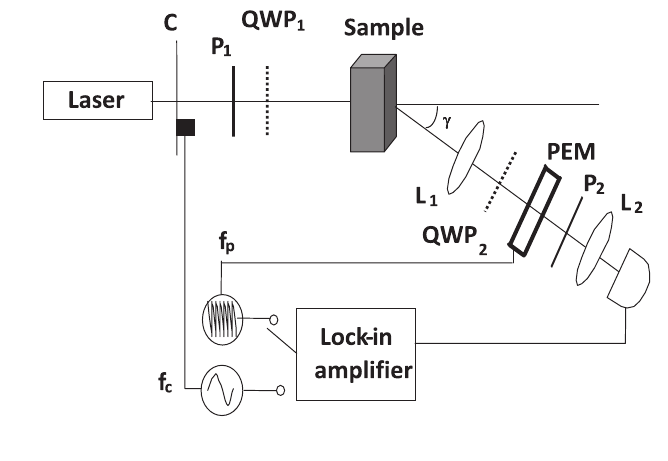
\includegraphics[width = 0.6\textwidth]{Chapter4/Figures/PMSDpolarimetry.png}	
	\caption[Polarimetry system proposed by Wood~et al.\,\cite{wood2008towards}]{Stoke polariemtry system using polarization modulation and a lock-in-amplifier. The image is taken form \cite{wood2008towards}.}
	\label{fig:pmodulationStokes}
	\end{figure}
In such a system, usually un-polarized light passes through the mechanical chopper and then the lock-in amplifier in order to establish its overall signal intensity levels. A linear polarizer ($P_{1}$), with or without a quarter wave plate ($QWP_{1}$) is used as input optics.
This set up is required in order to generate any of the four polarization states.
The detection path consists of a removable quarter wave plate ($QWP_{2}$) with its fast axis oriented at $-45^{\circ}$, a \ac{pem} and a linear polarizer, oriented at $45^{\circ}$.
The linear polarizer converts the \ac{pem} polarization modulation to intensity modulation suited for photodetection.
An interested reader is guided to the original article~\cite{wood2008towards} and Ghosh~et al.\,\cite{ghosh2011tissue} for further details regarding these systems.
%The PEM is a linearly birefringence resonant device, operating in $kHz$ range. The fast axis of the PEM is set to $0^{\circ}$ and its retardation is modulated according to the sinusoidal function $\delta_{PEM} = \delta_{0} \sin(\omega t)$. The $\delta_{0}$ is the user specified amplitude of the maximum retardation of $EPM$.


Besides the above methods for creating a full Stokes polarimetry system, a full Stokes image polarimetry system was proposed by Boulbry~et al.\,\cite{boulbry2006novel}.
The proposed spectro-polarimetric system is based on hemispherical backscattering for analysis of superficial skin lesions.
In order to remove the effect of rough skin backscattering and reflection, the proposed method is constructed with out-of-plane illumination~\cite{ramella2005out}.
The proposed system is composed of sixteen polarized light sources positioned over a hemisphere.
Each light source generates a collimated incident beam of blue, green or red illumination at the center of the hemisphere~\cite{boulbry2006novel}.
Figure \ref{fig:SVhemisphere} shows the position of the illumination source tubes (illuminators) over the hemisphere and the elements within each tube (a tri-color light emission diode, a thin film polarizer and a lens). 
	\begin{figure}
	\subfloat[]{%[width=0.3\textwidth]
	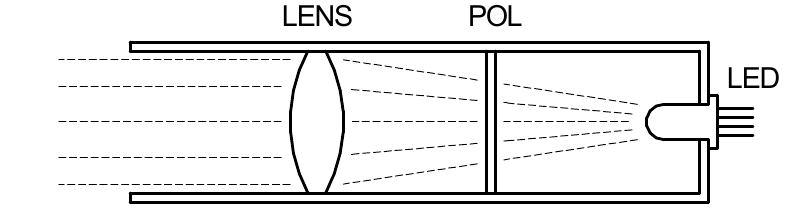
\includegraphics[width = 0.6\textwidth]{Chapter4/Figures/fig1hemisphere.png}
	}\ \hfil
	\subfloat[]{%[width=0.3\textwidth]
    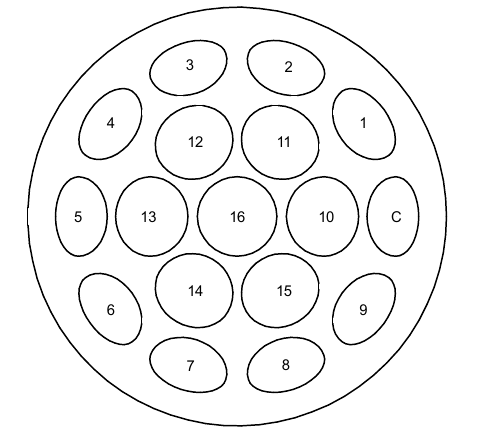
\includegraphics[height = 0.2\textheight , width = 0.35\textwidth]{Chapter4/Figures/fig2hemispher.png}
	}
	\caption[Polarimetric device proposed by \cite{boulbry2006novel}]{(a) The illumination tubeand (b) Sixteen illumination tubes and the camera $C$, on the surface of the hemisphere with respect to the normal of the sample. Images are taken from \cite{boulbry2006novel}.} 			 			    
	\label{fig:SVhemisphere}
	\end{figure}

\noindent A Stokes vector imaging is positioned on the shell at an oblique angle to the sample normal and consists of a 12 bits camera, two \ac{lc} and a fixed polarizer. 
Using seven retardance combinations of rotated crystal retarders, the four Stokes vectors were obtained~\cite{boulbry2006novel} via a least square solution, from which the polarized and unpolarized intensity of the light source as well as the parallel and perpendicular part of the polarized intensity were measured.
The method was only tested on a actinic keratosis and, unfortunately, was not tested on further skin lesions.


%Illuminators 1–9 and the camera are centered 49° from the surface normal, illuminators 10–15 are centered 24° from surface normal, and illuminator 16 is centered on the surface normal. The polarizers in illuminators 5, 10, 13, and 16 aligned 45° from the plane containing them, while those in the rest of the illuminators are aligned in the plane containing the respective illuminator and the surface normal.

%The authors used their implemented system for measuring the Stokes parameters and respectively the un-polaized image. They also suggest to divide the polarized part of the measurements into two categories of reference polarized intensity and cross-polarized reference intensity.  
%	
%	The measurement of four Stokes parameter was discussed in Sec. \ref{StokesMeasurement}. The explained set up was originally proposed by Collett et al. \cite{collett1984measurement}. This method was used by other researchers, such as \cite{ghosh2003depolarization,sankaran1999polarization,zhao2009,boulbry2006novel}, however when accurate quantification of the intrinsic tissue characteristics is required, a more sensitive approach should be considered. The sensitivity of the measurements can be improved by using a polarization modulation in combination with synchronous detection \cite{coa2004balanced,vitkin2002effects,studinski2000methodology,guo2006angular}. 
%	
%  	In \cite{coa2004balanced}, they demonstrate that it is possible to reduce the intensity noise and also direct measurements of Stokes parameters by using a amplitude or polarization modulation in combination with a phase-locked detector. 
%  	
% \cite{vitkin2002effects} used polarization modulation with a synchronize detection in the perpendicular and backscattering orientations to detect the scattered light from the liquid turbid samples containing varying amounts of left and right isometric forms of a chiral sugar. Their research was aimed towards non-invasive techniques of glucose sensing in diabetic patients.   
%
%A schematic of the experimental polarimetry system employing polarization modulation and synchronous detector with reference to \cite{guo2006angular,ghosh2011tissue} is shown in Fig.\ref{fig:PMSDpolarimetry}. In such a system, usually un-polarized light is passes through the mechanical chopper and then the lock-in amplifier in order to establish the overall signal intensity levels. A linear polarizer ($P_{1}$), with or without a quarter wave plate ($QWP_{1}$) is used as input optics. This set up is required in order to generate any of the four polarization states. The detection path consists of removable quarter wave plate ($QWP_{2}$) with its fast axis oriented at $-45^{\circ}$,  photoelastic modulator ($PEM$) and a linear polarizer, oriented at $45^{\circ}$. The linear polarizer converts the $PEM$ polarization modulation to intensity modulation suited for photo detection.
%
%The PEM is a linearly birefringence resonant device, operating in $kHz$ range. The fast axis of the PEM is set to $0^{\circ}$ and its retardation is modulated according to the sinusoidal function $\delta_{PEM} = \delta_{0} \sin(\omega t)$. The $\delta_{0}$ is the user specified amplitude of the maximum retardation of $EPM$.
%
%	\begin{figure}
%	\centering 
%	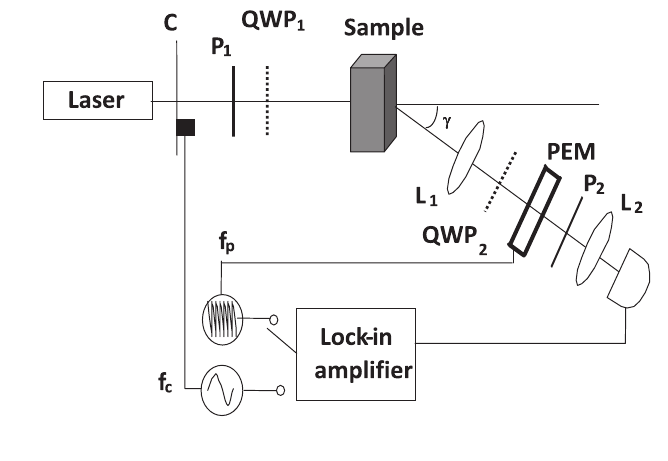
\includegraphics[width = 0.6\textwidth]{Chapter4/Figures/PMSDpolarimetry.png}	
%	\caption{ A schematic of the experimental polarimetry system with a polarization modulation and synchronous detector \cite{guo2006angular}}
%	\label{fig:PMSDpolarimetry}
%	\end{figure}

	
\subsection{Mueller polarimeter}
As explained earlier, Stokes vectors are not enough for measuring medium properties, so additional measurements and analysis is required.
The Mueller matrix provides these additional measurements at the cost of a more complicated setup.
This matrix and its parameters were explained in Sect.\,\ref{subsec:MuellerMeasurement}.
Sixteen elements of the Mueller matrix are measured via \acf{dc} sequential static measurements or \acf{ac} modulation based measurements \cite{ghosh2011tissue}.
In the latter approach, the four states of polarization (linear polarization at $0^{\circ}$, $45^{\circ}$, $90^{\circ}$ and rigth/left circular polaization $L$ and $R$) are applied individually as the input state, and the Stokes vector corresponding to each input is measured as an output.
The 16 elements of the Mueller matrix are then constructed using the measured Stokes vectors (see Eq. \ref{Eq:MuellerPolarimetry}) \cite{ghosh2009mueller}. 
	
	\begin{equation}\label{Eq:MuellerPolarimetry}
	\small
	M = 
	\begin{bmatrix}
	\frac{1}{2}(I_{H}+I_{V}) &  \frac{1}{2}(I_{H}-I_{V}) &  I_{P}-M(1,1) &  I_{R}-M(1,1)\\
    \frac{1}{2}(Q_{H}+Q_{V}) &  \frac{1}{2}(Q_{H}-Q_{V}) &  Q_{P}-M(2,1) &  Q_{R}-M(2,1)\\
	\frac{1}{2}(U_{H}+U_{V}) &  \frac{1}{2}(U_{H}-U_{V}) &  U_{P}-M(3,1) &  U_{R}-M(3,1)\\
	\frac{1}{2}(V_{H}+V_{V}) &  \frac{1}{2}(V_{H}-V_{V}) &  V_{P}-M(4,1) &  V_{R}-M(4,1)\\		
	\end{bmatrix}~,
	\end{equation}\\
	
\noindent where the four input states are denoted with $H$ for $0^{\circ}$, $V$ for $ 90^{\circ}$, $P$ for $45^{\circ}$, and $R$ for right circular polarized.
The Mueller matrix elements are represented by $M(i,j)$ with respect to their row and column.
This approach has been used by \cite{ghosh2009mueller,ghosh2008mueller}.
%The modulation/synchronous detection approach explained for Stokes polarimeter, can be used for Mueller polarimeter as well \cite{ghosh2009mueller,ghosh2009mueller}.

A dual rotating retarder approach is another way to generate the modulation-based Mueller matrix polarimeters \cite{ghosh2011tissue,goldstein1992mueller,azzam1978photopolarimetric,smith2002optimization}.
In this approach, the incident polarization states are generated by the \ac{psg} unit which contains a linear polarizer and a rotating linear retarder with retardance and angular speed of $\sigma_{1}$ and $\omega_{1}$, respectively.
The backscattered light from the sample are then analyzed by a \ac{psa} unit.
This unit contains a rotating linear retarder (retardance of $\sigma_{2}$ and angular speed of $\omega_{2}$) and a fixed linear polarizer in sequence.
In this set-up the axis of the polarizer and analyzer are kept parallel and the retardation of the two retarders is chosen to be the same $\sigma_{1} = \sigma_{2}= \pi/2$, while their angular frequencies differ from each other by five times ($\omega_{1} = \omega$, $\omega_{2} = 5\omega$ ).
The rotation of the retarders at different rates results in a modulation of a detected signal and encodes all the sixteen Mueller matrix elements into the amplitude and phases of 12 frequencies in the detected intensity signal.
The detected signal is Fourier analyzed and the Mueller matrix elements are constructed from the Fourier coefficients \cite{ghosh2011tissue,goldstein1992mueller,azzam1978photopolarimetric,smith2002optimization}. 

Dubreuil~et al.\,\cite{dubreuil2007snapshot} introduced another modulation-based Mueller matrix polarimeter, known as the Snapshot Mueller matrix.
The Snapshot system contains two linear birefringence retarders (wave plates) and a linear polarizer in the \ac{psg} unit and two birefringence retarders and a fixed linear polarizer (perpendicular to the one in the \ac{psg} unit) at the \ac{psa} unit (see Fig. \ref{fig:snaphotMueller}).
This technique measures the 16 elements of the Mueller matrix simultaneously by using wavelength polarization coding and decoding.
The resultant spectral signal is stored by the spectrometer and is Fourier analyzed in order to achieve the 16 elements of the Mueller matrix. 
	\begin{figure}
	\centering 
	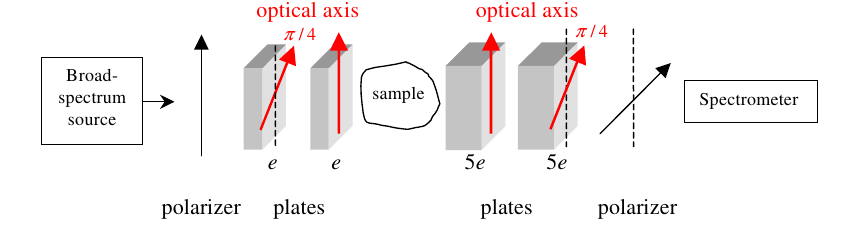
\includegraphics[width = 0.7\textwidth]{Chapter4/Figures/snapshotMueller.png}	
	\caption{ Snapshot Mueller polarimeter for the configuration, \cite{dubreuil2007snapshot}. }
	\label{fig:snaphotMueller}
	\end{figure}
\noindent In this system the \ac{psg} unit contains a linear polarizer at \ang{0} and two wave plates with their axis rotated at \ang{45} and \ang{0}, respectively.
The \ac{psa} unit contains two wave plates with their axis at \ang{0} and \ang{45}, respectively, and a linear polarizer at \ang{90}. 
One crucial parameter in this system is the choice of thickness of the birefringence plates.
The author proposed to having the birefringence in the \ac{psa} unit five times thicker than those in the \ac{psg}.

It should be noted that the Mueller polarimeters mentioned so far are suited for point polarimetry and are not applicable for large area imaging.
In this regard, several approaches are proposed and explained in the following.

Antonelli~\cite{antonelli2011biomedical} proposed three Mueller image polarimeters in her phd thesis; full Mueller imaging using focused illumination, Fourier space image polarimetry, and real space full Mueller imaging.
The latter system was proposed for thick tissue imaging while the two former, ones were designed for thinner tissue.
The first proposed instrument is shown in Fig.~\ref{fig:FIMueller}.
This system was implemented according to the system described by \cite{hielscher1997diffuse}.
Hielscher~et al.\,\cite{hielscher1997diffuse} developed the Mueller imaging system for analyzing the intensity patterns of backscattered light from the turbid media.
\begin{figure}[H]
\begin{center}
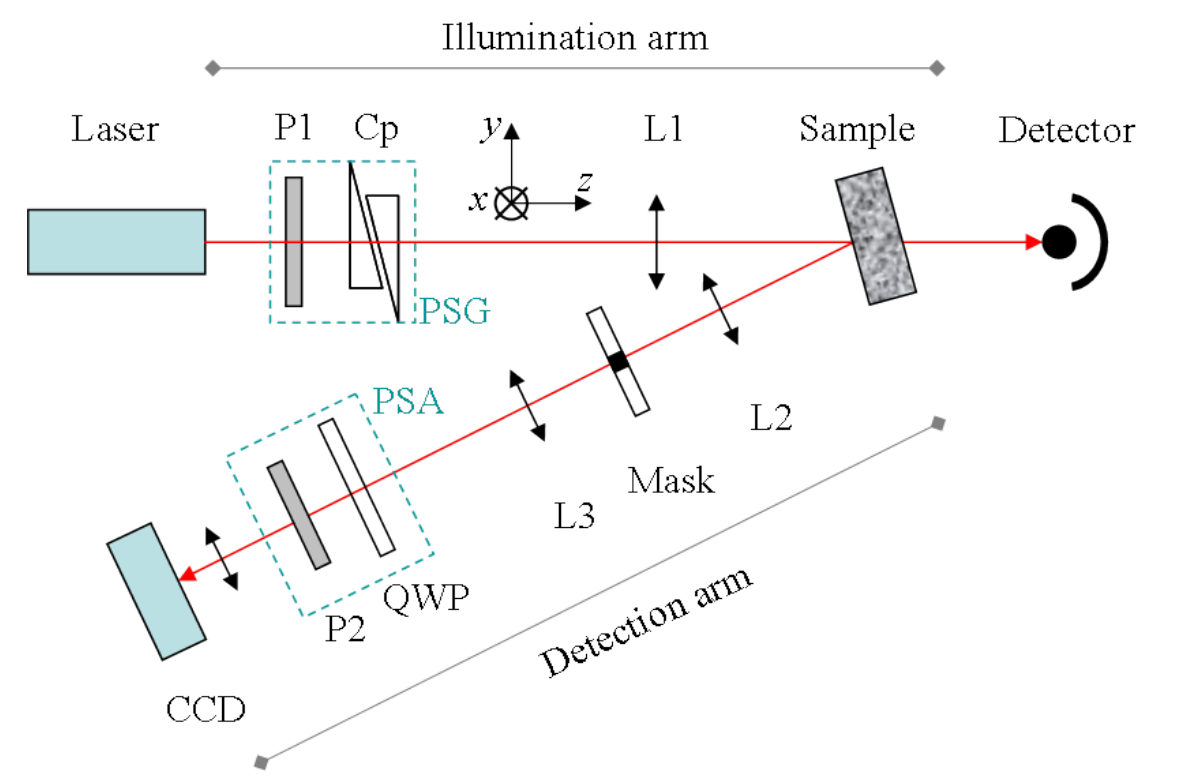
\includegraphics[width = 0.7\textwidth] {Chapter4/Figures/FIMueller.png}
\end{center}
\caption[Full Mueller polarimetry using focused illumination~\cite{antonelli2011biomedical}]{Full Mueller polarimetry system with focused illumination. The image is taken from \cite{antonelli2011biomedical}.}
\label{fig:FIMueller}
\end{figure}
\noindent The \ac{psg} unit of this system is composed of a linear polarizer ($P_{1}$) and a Babinet-Soleil-Bravais compensator (CP)~\cite{antonelli2011biomedical}, while the \ac{psa} unit is composed of a quarter wave plate (QWP) and a linear polarizer ($P_{2}$).
The compensator retardance is set to either \ang{180}, or \ang{90}.
The former is used to generate the linearly polarized states, and the later to generate circular polarized states.
In the \ac{psa} unit the QWP is set parallel to $P_{2}$ to measure the linear polarized state and it is rotated by \ang{45} to measure circular polarized states.
Using this setup, 36 raw images, corresponding to all the combinations of the polarization states possible in the \ac{psg} and \ac{psa} units, are acquired to complete the Mueller matrix. 
The final Mueller matrix, as a combination of the acquired 36 images, is shown in Fig.~\ref{fig:FIMuellermat}.
Here $O$ refers to an unpolarized state which is generated by the average of the two orthogonal state (i.e. H and V or P and M or L and R).
For each pair, for instance $HV$, the first element represents the polarization state of the \ac{psg} unit, while the polarization state of the \ac{psa} unit is represented by the second element.
\begin{figure}
\begin{center}
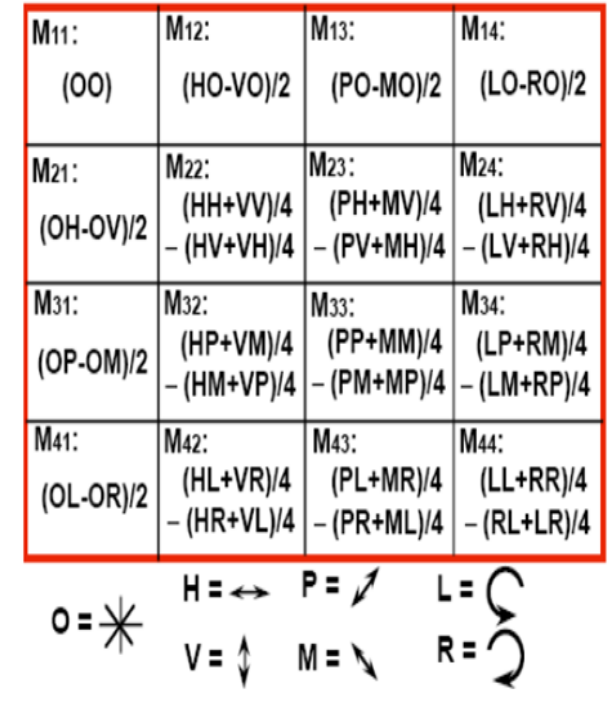
\includegraphics[width = 0.6\textwidth ]{Chapter4/Figures/FIMuellermat.png}
\end{center}
\caption[Mueller matrix obtained by full Mueller imaging with focused illumination system~\cite{antonelli2011biomedical}]{Mueller matrix as combination of 36 raw images acquired by full Mueller imaging with focused illumination setup~\cite{antonelli2011biomedical}.}
\label{fig:FIMuellermat}
\end{figure}

The second system, Fourier space image polarimetry, is shown in Fig.~\ref{fig:FSMueller}.
In this system, the \ac{psg} unit consists of a half wave plate (HWP), followed by a linear polarizer and QWP and the \ac{psa} unit contains one QWP followed by a linear polarizer.
Table~\ref{tab:AntonelliTable} illustrates the existence and rotation of each of the optic elements in the \ac{psg} and \ac{psa} units for creating different polarization states.
It should be noted that the polarization states generated in the \ac{psg} unit are independent from those generated in the \ac{psa} unit.

\begin{table}
\caption[Polarized state generator and \ac{psa} units setting proposed by \cite{antonelli2011biomedical}]{Setting for the \ac{psg} and \ac{psa} units for generating 6 polarization states in each unit~\cite{antonelli2011biomedical}.}
\begin{center}
\scriptsize{
\resizebox{0.7\textwidth}{!}{
\begin{tabular}{c ccc c	cc}
\toprule 
 & \multicolumn{3}{c}{\ac{psg}} &  & \multicolumn{2}{c}{\ac{psa}}\\
 \cmidrule{2-4} \cmidrule{6-7}
Polarization states & HWP & P & QWP & & QWP & P \\
\midrule
H & \ang{0} & \ang{0} & removed & & removed & \ang{0}\\
V & \ang{45} & \ang{90} & removed & & removed & \ang{90}\\
P & \ang{45} & \ang{45} & removed & & removed & \ang{45}\\
M & \ang{45} & \ang{315} & removed & & removed & \ang{135}\\
R & \ang{45} & \ang{90} & \ang{45} & & \ang{45} & \ang{0}\\
L & \ang{45} & \ang{90} & \ang{-45} & & \ang{-45} & \ang{90}\\
\bottomrule

\end{tabular}}}
\end{center}
\label{tab:AntonelliTable}
\end{table}

\begin{figure}
\begin{center}
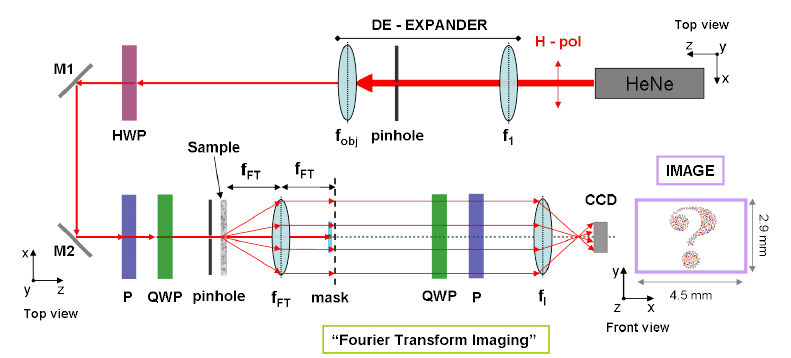
\includegraphics[width = 0.9\textwidth]{Chapter4/Figures/FourierTransformImaging.png}
\end{center}
\caption[Fourier space Mueller polarimetry~\cite{antonelli2011biomedical}]{ Fourier space Mueller polarimetry system proposed by \cite{antonelli2011biomedical}.}
\label{fig:FSMueller}
\end{figure}
\noindent Using the 36 raw images with different polarization states, the author also proposed using a so called polarimetric matrix ($6 \times 4$), whose columns are the components of the normalized Stokes vector and the lines are the input polarization states (see Fig.~\ref{fig:PM}).
Similar to the Mueller matrix (see Fig.~\ref{fig:FIMuellermat}), the polarization state of the \ac{psg} unit is represented by the first element while the second element shows the polarization state of the \ac{psa} unit.
	\begin{figure} [h]
	\centering 
	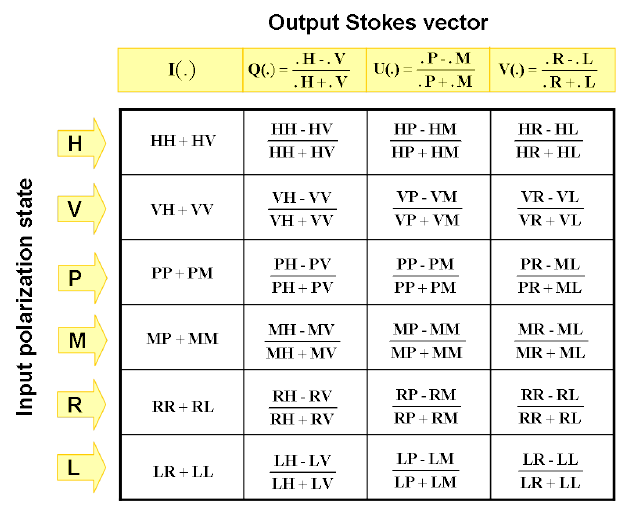
\includegraphics[width = 0.8\textwidth]{Chapter4/Figures/PolarimetricMatrix.png}	
	\caption[Polarimetric matrix]{Polarimetric matrix defined with Fourier space imaging~\cite{antonelli2011biomedical}. }
	\label{fig:PM}
	\end{figure}
	
The third system, real space full Mueller imaging, similar to \cite{de2004general} uses two \ac{lc} to eliminate the need of manual rotation of the optical parts in the \ac{psg} and \ac{psa} units (see Fig.~\ref{fig:RSMueller}).
This system was used for imaging ex-vivo cone biopsies.
	\begin{figure}[h]
	\centering 
	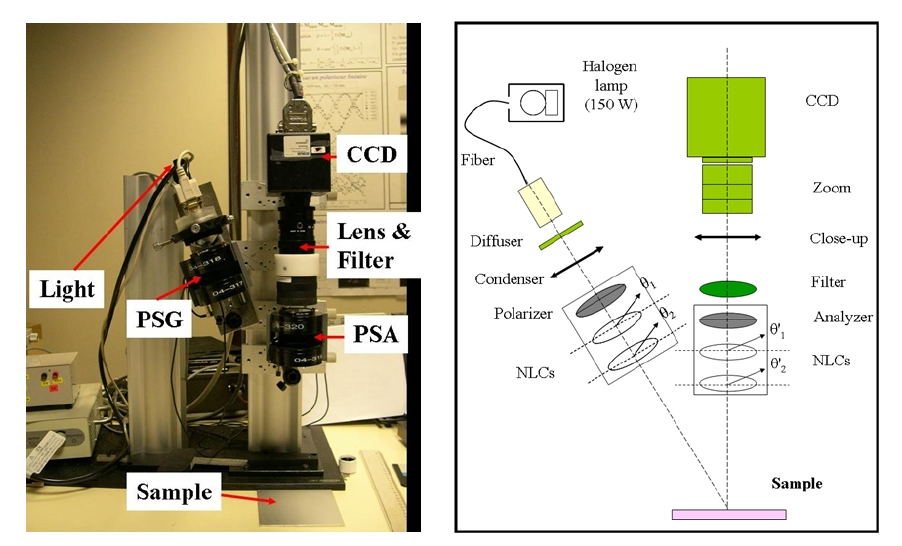
\includegraphics[width = 0.9\textwidth]{Chapter4/Figures/RealMuellerImagingSystem.png}	
	\caption[Real spape Mueller imaging proposed by \cite{antonelli2011biomedical}]{ The real space Mueller imaging system proposed by \cite{antonelli2011biomedical}. }
	\label{fig:RSMueller}
	\end{figure}

\noindent In this system, the \ac{psg} unit consists of a linear polarizer and two \ac{lc} elements and the \ac{psa} unit contains the same elements in reverse order (i.e. two \ac{lc} and then a linear polarizer).
Using different rotation angles for the two \ac{lc} allows to obtain the four polarization states for the \ac{psg} and \ac{psa} units (common choice of angles, $\theta_{1} = \ang{45}$, and $\theta_{2} = \ang{0}$).
Consider the four incident polarization states of the \ac{psg} unit as $4 \times 4$ matrix $W$ (polarization states as columns) and the four basic states of the \ac{psa} unit as $4 \times 4$ matrix $A$ (polarization states as rows).
Then the 16 raw data are the elements of a $4 \times 4$ real matrix $B$ (measurement matrix) such as~\cite{de2004general, antonelli2011biomedical}:
	\begin{equation}
	\label{eq:LCMuellerEq}
	B = AMW~,
	\end{equation}
\noindent where $M$ is the Mueller matrix of the sample.
Having the initial knowledge of the $A$ and $W$ matrices and measuring the $B$ matrix, the Mueller matrix $M$ is calculated.
The two matrices of $A$ and $W$ are known through the calibration procedure~\cite{compain1999general}.
%This matrix is obtained by measuring the $B$ matrix and  which can be calculated by measuring the $B$ matrix and having the initial knowledge of $A$ and $W$.
%The two matrices of $A$ and $W$ are known if the system is calibrated~\cite{compain1999general}.

Besides the aforementioned systems, Mueller polarimetry was used in several other studies to capture images of human and animal tissues~\cite{twietmeyer2008mueller,li2009mueller}.

Li~et al.\,\cite{li2009mueller} proposed another ex-vivo instrument to characterize muscle depolarization properties.
Comparing relax and stretch muscles and polystyrene solution, the authors concluded that the polarization properties of a muscle are clearly different from the polystyrene solution.
However, despite clear changes in raw polarization references, muscle stretching shows minimal changes in terms of its polarization properties. 

Twietmeyer~et al.\,\cite{twietmeyer2008mueller} proposed a Mueller polarimetry system for in-vivo imaging of the retina and tested their proposed method on 15 normal subjects.
The authors proposed adjusting the available scanning laser polarimeter GDx by using two \ac{lc} in the \ac{psg} and \ac{psa} units in order to change the polarization states.
Although no subjects with retinal diseases were evaluated, the authors concluded that the proposed system is well suited for monitoring the thickness of the nerve fiber and Henle layers and can be used as an indicator of the presence and progression of glaucoma~\cite{twietmeyer2008mueller}.




% Such a system will have lower sensitivity so alternative methods have been considered for instance using a liquid crystal variable retarders ($LC$) instead of manually rotating the optical parts of the PSG and PSA \cite{de2004general} (see Fig \ref{fig:LCMueller}).  The PSG unit of this system consists of a linear polarizer ($P_{1}$) and two liquid crystal variable retarders ($LC_{1}$, $LC_{2}$) with two retardance value of $\sigma_{1}$ and $\sigma{2}$ respectively. The PSA unit have a similar structure to PSG unit ($LC_{3}$, $LC_{4}$ and $P_{2}$) with the reverse order and the detection device at the end, in this case a CCD, for image acquisition. The structure of the LC polarimeter can be seen in Fig \ref{fig:LCMueller}.
%	\begin{figure} 
%	\centering 
%	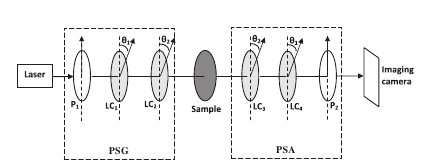
\includegraphics[width = 0.8\textwidth]{Chapter4/Figures/LCMueller.png}	
%	\caption{$LC$ Mueller matrix polarimeter \cite{ghosh2011tissue} }
%	\label{fig:LCMueller}
%	\end{figure}

%Usually the birefringence axis of the two retarders are kept at angles $\theta_{1}$ and $\theta_{2}$ respectively with reference to the axis of the polarizer $P_{1}$. (Generally the angles are chosen as: $\theta_{1} = 45 ^{\circ}$ and $\theta_{2} = 0 ^{\circ}$). Considering the optics elements order in the PSG unit, once can conclude how the incident polarizer states can be related to $\sigma_{1}$ and $\sigma_{2}$. This relation is illustrated in Eq.\ref{Eq:LCMuellerEq}.
%
%	\begin{equation}\label{Eq:LCMuellerEq}
%	\small
%	\begin{pmatrix} 
%	I_{f}\\
%	Q_{f}\\
%	U_{f}\\	
%	V_{f}\\
%    \end{pmatrix} = 		
%	\begin{pmatrix}
%	1 & 0 & 0 & 0 \\
%	0 & 1 & 0 & 0 \\
%	0 & 0 & \cos \sigma_{2} &  \sin \sigma_{2}\\
%	0 & 0 & -\sin \sigma_{2} &  \cos \sigma_{2}\\
%	\end{pmatrix}
%	\begin{pmatrix}
%	1 & 0 & 0 & 0 \\
%	0 & \cos \sigma_{1} & 0 & -\sin \sigma_{1} \\
%	0 & 0 & 1 & 0 \\
%	0 & \sin \sigma_{1} & 0 & \cos \sigma_{1} \\
%	\end{pmatrix} 
%	\begin{pmatrix}
%	1\\
%	1\\
%	0\\
%	0\\
%	\end{pmatrix} = 
%	\begin{pmatrix}
%	1 \\
%	\cos\sigma_{1}\\	
%	\sin \sigma_{2} \sin \sigma_{1}\\	
%	\cos \sigma_{2} \sin \sigma_{1}\\
%	\end{pmatrix}	
%	\end{equation} 

%%%The calibration of a system like the imaging polarimeter we are describing is a very
%%%difficult task by the usual approach involving a detailed model of the instrument, as this
%%%system is a "stack" of many elements, each of which may introduce serious artefacts which
%%%may be difficult to understand and model properly.
%%%A very different approach has been followed at LPICM [70] to develop the eigenvalue
%%%calibration method (ECM), which has been successfully used on many different Mueller
%%%polarimeters. Without getting into details, which would be outside the scope of this
%%%manuscript, this method can accurately retrieve the matrices W and A from four mea-
%%%surements on calibration samples by linear algebra techniques, without any modelling of
%%%the instruments. Moreover, the calibration samples are not very specific (typically one
%%%can use linear polarizers, retardation plates other than half wave) and do not need to be
%%%accurately known, as they are characterized during the calibration procedure itself. Of
%%%course, our imaging polarimeter was calibrated at each wavelength by using ECM, and
%%%provided polarimetric images with a typical maximum error of the order of 0.02 to 0.03
%%%on the normalized elements Mij ∗
%%% = Mij /M11, i, j = 1..4 i · j = 1.

%	\begin{figure}
%	\begin{center}
%	\subfloat[]{
%	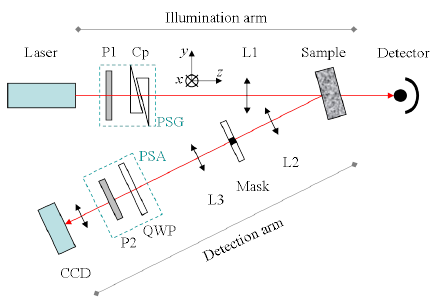
\includegraphics[width = 0.7\textwidth]{Chapter4/Figures/illuminationMueller.png}
%	\label{fig:focusedMueller}
%	}\  \\
%	\subfloat[]{%[width=0.3\textwidth]
%    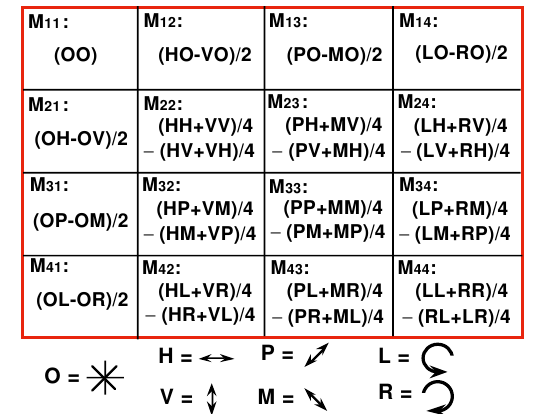
\includegraphics[width = 0.7\textwidth]{Chapter4/Figures/illuminationMueller_table.png}
%    \label{fig:illuminationMuellerTable}
%	}
%	\caption{(a)Full Mueller imaging system (b) Combination of the raw images for calculating the Mueller matrix elements   \cite{antonelli2011biomedical,hielscher1997diffuse}} 	
%	\end{center}
%	\end{figure}












\section{Conclusion}
The basics of polarization, how to exploit polarization and its parameters in bio-imaging and skin screening and the recent state of the art techniques were discussed. 
It was shown that partial or full Stokes and Mueller polarimetry allow screening which is of main interest. 
However as it was discussed, Mueller and full polarimetry systems are difficult to adjust for in-vivo screening. 
Therefore as the first step, we consider to exploit partial polarimetry and develop our \ac{pd} accordingly.
This device is further explained in Chap.\,\ref{chp:chapter5}.

%%In this chapter we presented the basics of polarization, different approaches of empoloying polarization and polarized parameters in bioimaging and 

%%% Local Variables: 
%%% mode: latex
%%% TeX-master: "../thesis"
%%% End: 

\clearemptydoublepage
\acresetall
\chapter{Machine Learning and Classification Principles}
\label{chp:chapter2}
\section{Introduction} \label{sec:chp2-sec1}
Machine learning is refers to a set of methods that can automatically detect patterns in data and use them in decision making and future data prediction~\cite{murphy2012machine}. 
Machine learning techniques are usually divided into two groups: descriptive (or unsupervised) and predictive (or supervised) learning.

Unsupervised learning intends to find ``interesting structures'' in a given data without any additional information about the expected output. 
These techniques formulate their problems as unconditional density estimation and multivariate probability models. 
Clustering approaches and dimension reduction methods, \acf{pca}, and graph structures are two examples of unsupervised learning.   

Supervised learning intends to find a mapping $f(.)$ which relates a set of inputs $x$ to a set of outputs $y$. 
The learning is comprehended using a set of $N$ samples and their labels $D = \{(x_{i}, y_{i})\}^{N}_{i = 1}$, called the training set.
The samples $x_{i}$ can vary from 2-D points in Cartesian coordinates to more complex forms such as images, sentences, time series, graphs, etc.
Similarly, the labels $y_{i}$ can be represented by any structure, however, in most methods they are considered to be either categorical or numerical. 
Supervised learning is known as a classification problem when $y_{i}$ is categorical; and when $y_{i}$ is a real value the problem is referred to as regression~\cite{murphy2012machine}. 

In this research, we are interested in supervised learning, and the classification problem in particular. 
Classification aims to map a set of inputs to a set of outputs, where the outputs are divided into different classes, $y \in \{1,...,C\}$.
%{\color{green}As previously mentioned classification aims to maps a set of input $x$ to a set of output $y$, where $y \in \{1,...,C\}$ and C is the number of classes.} 
If $C = 2$, it is a binary classification problem, while $C > 2$ makes it a multiclass classification. 
This project aims to separate melanoma from all other pigmented skin lesions, thus addressing a binary classification problem. 

Classification has numerous applications in real life.
Some of the most common and challenging areas include email spam filtering, data mining, face detection and recognition, document classification, and the problem of cancer detection among others.
In order to solve a classification problem, a framework consisting of several generic steps is required.
Figure~\ref{fig:GCF} shows such a general framework whose steps are described in the following sections of this chapter. 
Due to the broad studies of \ac{cad} systems of melanoma using dermoscopic images, in comparison to Stokes polarimetry, each step covers the state of the art related to conventional dermoscopic approaches.

%\tikzstyle{block} = [rectangle, draw, fill= blue!20,
%   text width=7em, text centered, rounded corners, minimum height=4em , minimum width = 7em]
%\tikzstyle{line} = [draw, -latex']
%\tikzstyle{block2} = [rectangle, draw, fill=gray!20,
%    text width=7em, text centered, rounded corners, minimum height=4em, minimum width = 7em]
%\tikzstyle{block3} = [rectangle, draw, fill=blue!40,
%    text width=7em, text centered, rounded corners, minimum height=3em , minimum width = 7em]
%\def\blockdist{1}
%\def\edgedist{1.5}
    \tikzstyle{block} = [rectangle, draw, fill=blue!30,text = black,
    text width=6em, text centered, rounded corners, minimum height=4em , minimum width = 7em]
    \tikzstyle{line}=[draw, -latex']
	\tikzstyle{block2} = [rectangle, draw, fill=white!20,
    text width=6em, text centered, rounded corners, minimum height=4em, minimum width = 7em]
    \tikzstyle{block3} = [rectangle, draw, fill=blue!30, text = black,
    text width=7em, text centered, rounded corners, minimum height=4em , minimum width = 7em]
\def\blockdist{1}
\def\edgedist{1.5}
\begin{figure}
\centering   
\begin{tikzpicture}[node distance = 1cm,scale=0.8, every node/.style={scale=0.8}]
    % Place nodes
	\node[block2] (input) {Input Data}; 
	\node[block, right of= input , node distance = 3cm](pp){Pre-processing};
	\node[block, right of = pp, node distance = 3 cm](fe){Feature extraction}; 
	\node[block, right of = fe, node distance = 3 cm](fr){Feature representation}; 
	\node[block, right of = fr, node distance = 3 cm](db){Data balancing}; 
	\node[block, right of = db, node distance = 3 cm](clas){Classification}; 
	
	% --- The arrows 
	
	%\path(pp)+(-0.8,0) node (n) {};
	\path [line] (input) -- (pp);
    \path [line] (pp) -- (fe);
    \path [line] (fe) -- (fr);
    \path [line] (fr) -- (db);
    \path [line] (db) -- (clas);
   

\end{tikzpicture}
\caption[General classification framework]{General classification framework.}
\label{fig:GCF}
\end{figure}
 

\section{Preprocessing} \label{sec:chp2-sec2}
Data preprocessing is an essential and important step in machine learning. 
This step ensures the quality of the data before further analysis and serves to compensate their imperfections. 
Thus, preprocessing acts as a foundation and assures precision in the developed framework.
In our research, samples are represented by images that must be preprocessed prior to further analysis to account for artifacts and variations in the images acquisition.
Moreover, despite that some studies treated image segmentation as an individual step~\cite{barata2013towards,capdehourat2009pigmented,celebi2007methodological}, we consider it as part of the preprocessing step, alongside image enhancement, denoising, and hair removal.
%Image enhancement, hair removal and segmentation are explained in the following as part of the preprocessing step.

%However in some studies it is treated as individual step.
%Image enhancement, hair removal and segmentation are explained in the following as part of preprocessing step.


\subsection{Image enhancement}\label{subsec:pp-enh}
Image enhancement is a set of adjustment processes on an image that make it more suitable for a specific application. 
Histogram equalization, gamma transformation, contrast and edge enhancement, illumination correction, white and color balancing, color calibration, as well as denoising belong to image enhancement techniques. 
%Contrast and edge enhancement or smoothing can be applied in frequency or spatial domain. 
In the field of skin imaging, among the aforementioned techniques, median filtering is mostly used to suppress noise, bright spots, reflections and small pores on the skin ~\cite{Chiem2007,Berenguer2009,Ruiz2011}. 
While this technique removes certain noise and artifacts, it also smooths the texture and border of the lesion, which is undesirable. 
%Probably, from lesion diagnosis point of view, the most important enhancement which can be applied is color calibration and correction. 
From the lesions diagnosis point of view, perhaps the most important enhancement concerns color calibration and correction. 
This operation aims to recover real colors of an image, allowing for more reliable use of color information in manual and automatic diagnosis~\cite{korotkov2012computerized}. 
The need for color correction while using the \acf{jpeg} format as opposed to RAW images was recently highlighted in~\cite{Quintana2011,Wighton2011a,celebiautomated}.
Figure~\ref{fig:Quintana1} shows \acf{awb}, \acf{cwb} and \ac{jpeg} color calibrated dermoscopic images acquired with two polarized cameras, while 
Fig.~\ref{fig:Quintana2} demonstrates the importance of calibrating RAW data in comparison with \ac{jpeg} dermoscopic images.



\begin{figure}
\centering
\subfloat[\ac{awb}]{
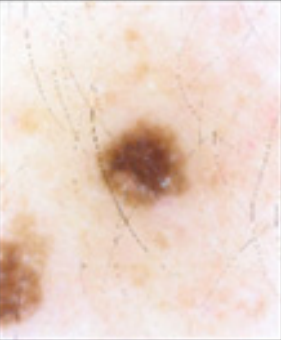
\includegraphics[height = 0.18\textheight, width= 0.16\textwidth]{Chapter2/Figures/quintana-awb_ex1.png}}\
\subfloat[\ac{cwb}]{
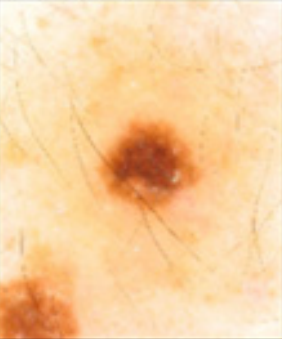
\includegraphics[height = 0.18\textheight, width= 0.16\textwidth]{Chapter2/Figures/quintana-cwb_ex1.png}}\
\subfloat[calibrated]{
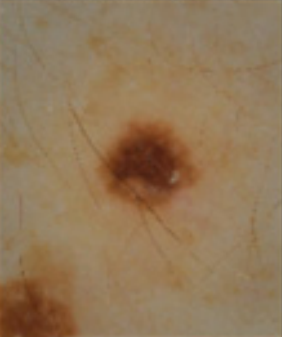
\includegraphics[height = 0.18\textheight, width= 0.16\textwidth]{Chapter2/Figures/quintana-calibrated_ex1.png}}\\
\subfloat[\ac{awb}]{
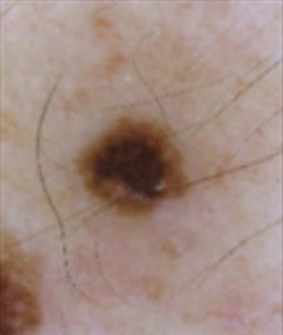
\includegraphics[height = 0.18\textheight, width= 0.16\textwidth]{Chapter2/Figures/quintana-awb_ex2.png}}\
\subfloat[\ac{cwb}]{
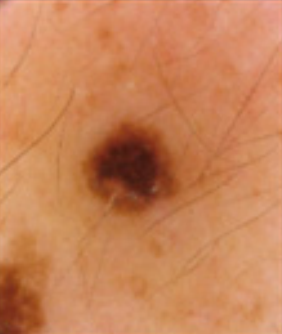
\includegraphics[height = 0.18\textheight, width= 0.16\textwidth]{Chapter2/Figures/quintana-cwb_ex2.png}}\
\subfloat[calibrated]{
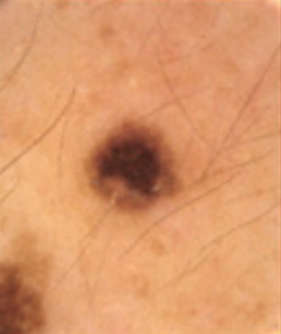
\includegraphics[height = 0.18\textheight, width= 0.16\textwidth]{Chapter2/Figures/quintana-calibrated_ex2.png}}
\caption[Color variations of dermoscopic images]{Variation in color depending on \Ac{awb}, \Ac{cwb} and \ac{jpeg} color calibration between images taken from two different dermoscopes. Images in the first row were taken with a Canon-A640 polarized dermoscope and the images in the second row were acquired with a Canon-G7 polarized dermoscope. Images are taken from~\cite{Quintana2011}.}
\label{fig:Quintana1}
\end{figure} 
 
\begin{figure}
\centering
\subfloat[\ac{cwb}]{
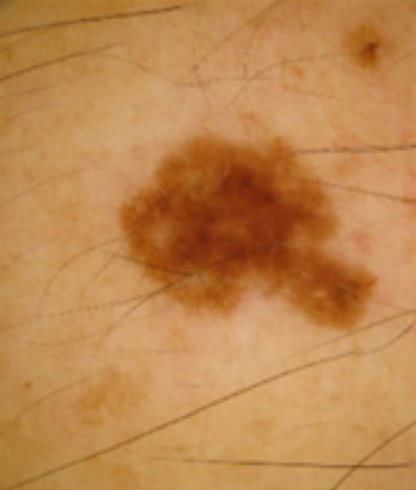
\includegraphics[height = 0.2\textheight, width= 0.19\textwidth]{Chapter2/Figures/quintana_cwb_ex3.png}}\
\subfloat[Calibrated-\ac{jpeg}]{
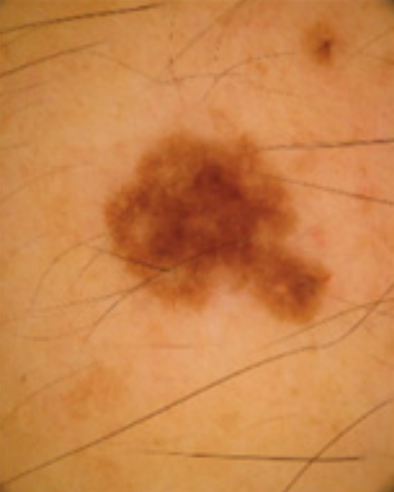
\includegraphics[height = 0.2\textheight, width= 0.19\textwidth]{Chapter2/Figures/quintana_JPEGCal_ex3.png}}\
\subfloat[Calibrated-RAW]{
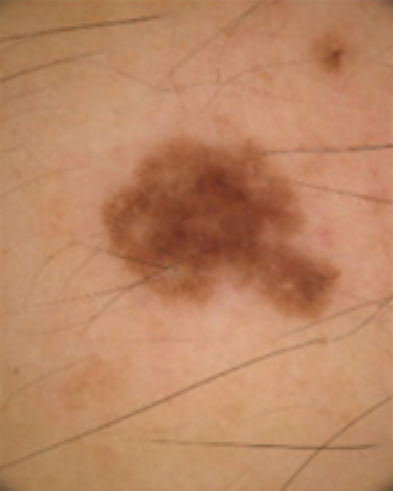
\includegraphics[height = 0.2\textheight, width= 0.19\textwidth]{Chapter2/Figures/quintana_RAWCal_ex3.png}}\\
\subfloat[\ac{cwb}]{
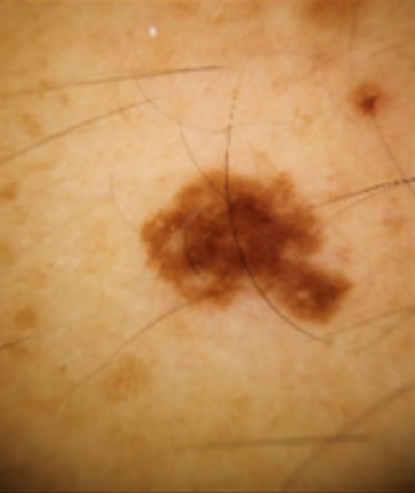
\includegraphics[height = 0.2\textheight, width= 0.19\textwidth]{Chapter2/Figures/quintana_cwb_ex4.png}}\
\subfloat[Calibrated-\ac{jpeg}]{
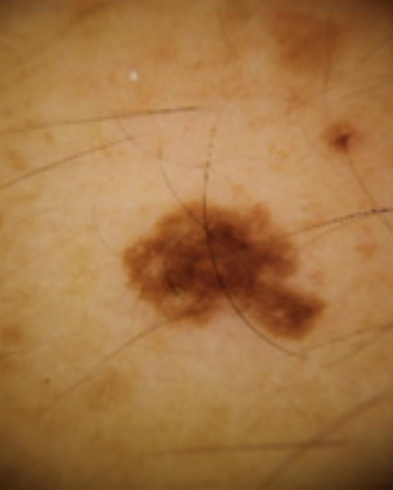
\includegraphics[height = 0.2\textheight, width= 0.19\textwidth]{Chapter2/Figures/quintana_JPEGCal_ex4.png}}
\subfloat[Calibrated-RAW]{
\includegraphics[height = 0.2\textheight, width= 0.19\textwidth]{Chapter2/Figures/quintana_RAWCal_ex4.png}}
\caption[Color variations between calibrated \ac{jpeg} and RAW images]{Variations in color between \Ac{cwb}, calibrated \ac{jpeg} and calibrated RAW images obtained with 2 different polarized dermoscopes. Images in the first row were acquired with Canon-G9 polarized dermoscope, while those in the second row were acquired with a Canon-5D polarized dermoscope. Images were taken from~\cite{Quintana2011}.}
\label{fig:Quintana2}
\end{figure}

\subsection{Artifacts removal} \label{subsec:artifactsremov}
Artifacts removal refers to noise removal in most image processing applications. 
However, in the field of skin imaging, it generally refers to elimination of hair, skin pores, ruler marks, air bubbles and specular reflections (see Fig.\ref{fig:artifacts}).
\begin{figure}
\centering
\subfloat[]{\includegraphics[height = 0.2\textheight, width= 0.3\textwidth]{Chapter2/Figures/artifacts-Hair-airbubble-Ruler.png}}\
\subfloat[]{\includegraphics[height = 0.2\textheight, width= 0.3\textwidth]{Chapter2/Figures/artifacts-SpecularReflection.png}}
\caption[Artifacts in dermoscopic images]{Artifacts in dermoscopic images: (a) hair, air bubbles and ruler marks, (b) specular reflection. The images are taken from Zhou~et al.\,\cite{Zhou2008a} and Gutenev~et al.\,\cite{Gutenev2001}, respectively.}
\label{fig:artifacts}
\end{figure}
Among these operations, hair removal is the most common and necessary step.  
If a lesion is occluded by hairs, their removal is essential to achieve correct segmentation and texture analysis.
To avoid digital hair removal, the patients are usually asked to shave before image acquisition.

A hair removal algorithm commonly consists of two steps: hair detection and hair restoration (or ``inpainting'')~\cite{korotkov2012computerized}.
Inpainting fills the image space previously occupied by hairs with estimated intensity/color values. 
Considering that original colors and borders of a lesion play an essential role in lesion diagnosis, intensity estimation of missing pixels is crucial and the best inpainting method should be applied. 
\begin{figure}
\hspace*{\fill}
\subfloat[]{
\includegraphics[height= 0.33\textheight, width= 0.3\textwidth]{Chapter2/Figures/Abas-comparison-original.png}}\hfill
\subfloat[]{
\includegraphics[height= 0.33\textheight, width= 0.3\textwidth]{Chapter2/Figures/Abas-comparison-mask.png}}\hfill
\subfloat[]{
\includegraphics[height= 0.33\textheight, width= 0.3\textwidth]{Chapter2/Figures/Abas-comparison-dullruze.png}}
\hspace*{\fill}\\
\hspace*{\fill}
\subfloat[]{
\includegraphics[height= 0.33\textheight, width= 0.3\textwidth]{Chapter2/Figures/Abas-comparison-d.png}}\hfill
\subfloat[]{
\includegraphics[height= 0.33\textheight, width= 0.3\textwidth]{Chapter2/Figures/Abas-comparison-e.png}}\hfill
\subfloat[]{
\includegraphics[height= 0.33\textheight, width= 0.3\textwidth]{Chapter2/Figures/Abas-comparison-fastmarching.png}}
\hspace*{\fill}
\caption[Comparison of inpainting methods]{Comparison of state of the art inpainting methods for hair removal algorithms. (a) Original image, (b) Highlighted hair mask, (c) DullRazor, (d) \ac{pde} non-linear inpainting, (e) exemplar-based inpainting, and (f) fast marching inpainting. The images are taken from \cite{Abbas2011a}.}
\label{fig:Abas-Comparison-repair}
\end{figure}
Lee~et al.\,\cite{Lee1997} proposed the first hair removal algorithm, DullRazor\textsuperscript{\textregistered}, for dermoscopic images. 
Kiani and Sharafat~\cite{Kiani2011} improved this algorithm to remove light-colored hairs as well as dark. 

Considering hair detection as a pixel classification problem, supervised learning was also applied in some studies~\cite{Debeir1999,Wighton2011}.
A recent survey on the topic was published by Abbas~et al.\,\cite{Abbas2011a}, where he reviewed the existing methods and proposed a broad classification based on the inpainting algorithms employed~\cite{korotkov2012computerized}: linear interpolation techniques~\cite{Lee1997,Fleming1998,Schmid-Saugeon2003,Nguyen2010}, inpainting by nonlinear \ac{pde}-based diffusion algorithms~\cite{Chung2000,Barcelos2009,Xie2009,Abbas2010a} and exemplar-based methods~\cite{Zhou2008a,Wighton2008,Abbas2010}. 
The authors~\cite{Abbas2011a,Abbas2012b} also proposed their own inpainting method based on fast marching inpainting. 
Figure~\ref{fig:Abas-Comparison-repair} shows an example demonstrating the results they achieved using different inpainting techniques.

\subsection{Image segmentation} \label{subsec:imgseg}
Image segmentation aims to decompose the image into meaningful parts with respect to a unique application. 
This technique uses image information such as grey level, texture, and color to divide the image into non-overlapping parts. 
Based on the information used, segmentation techniques are divided into four main groups: region-based, edge-based, clustering-based, and texture-based methods. 
Segmentation is also achievable via supervised learning. 

In automatic detection of melanoma, border delineation of the lesions is achieved by segmentation.
This is a challenging task due to variations in color, size, shape and texture of \ac{psls}, as well as occlusions and artifacts. 
In addition to the aforementioned challenges, segmentation algorithms face a problem of ground truth.  
%Moreover, due to difference of opinion among dermatologists and the fact that they do not require to delineate the lesion borders for their diagnosis~\cite{Day2001}, there is a ground truth problem.
It is very difficult to have a unique ground truth because dermatologists do not need to delineate lesion borders to make a diagnosis, and moreover, their individual delineations may vary significantly (see Fig.~\ref{fig:GTproblem}). 
So, normally the ground truth is generated as a fusion of different delineations done by experts. 
\begin{figure}
\centering
\subfloat[]{\includegraphics[height = 0.2\textheight, width= 0.3\textwidth]{Chapter2/Figures/Iyatomi-GT-original.png}}\	
\subfloat[]{\includegraphics[height = 0.2\textheight, width= 0.3\textwidth]{Chapter2/Figures/Iyatomi-GT-5D.png}}
\caption[Lesion delineation variations]{Example of manual delineation of clark nevus by 5 dermatologists. (a) Dermoscopy image, (b) Delineation by 5 dermatologists. Images are taken from Iyatomi~et al.\,\cite{Iyatomi2006}.}
\label{fig:GTproblem}
\end{figure}
Despite these challenges, numerous methods were proposed by the research community to tackle this problem.
Good comparisons of segmentation methods for dermoscopy images were published by Silveira~et al.\,\cite{silveira2009comparison}, Celebi ~et al.\,\cite{Celebi2009a}, and Ferreira~et al.\,\cite{ferreira2013wide}.  %Korotkov~et al.\,\cite{korotkov2012computerized}
The proposed methods can be categorized based on different criteria, for instance, technical properties, level of automation or their complexity.
A review of all the proposed methods is beyond the scope of this research. 
However, an overview of available reviews and certain approaches is presented in the following.

Thresholding was one of the first approaches applied to lesion segmentation.
This technique was applied in a single color channel at first~\cite{Gutkowicz-Krusin1997,Fleming1998} and then evolved to more sophisticated approaches such as iterative thresholding~\cite{Rajab2004}, type-2 fuzzy logic based thresholding~\cite{Yuksel2009}, fusion of thresholds~\cite{Celebi2009c,Celebi2010, Celebi2013}, hybrid~\cite{Garnavi2011}, local entropy~\cite{Abbas2013a} and color histogram thresholding~\cite{Peruch2013}.

Among the many segmentation approaches developed, a variety of methods were employed such as clustering~\cite{Schmid1999b, Zhou2009, Mete2011, Liu2012}, active contours~\cite{Yuan2009, Zhou2011a,Erkol2005}, supervised learning~\cite{Debeir1999, Wighton2011, Wighton2011b, Zortea2011}, and dynamic programming~\cite{Abbas2012}, just to name a few~\cite{korotkov2012computerized}.

It is clear that without a common dataset, a comparison of the proposed methods cannot be made. 
In this regard, some studies surveyed a comparison of several methods on their own datasets~\cite{Hance1996,Silveira2009,Celebi2007,Celebi2008a,ferreira2013wide}.

Six segmentation methods (split-and-merge, center split, multiresolution, fuzzy c-mean, PCT/median cut and adaptive thresholding) were compared in~\cite{Hance1996}, where the two latter approaches outperformed the others~\cite{korotkov2012computerized}.
Silveira~et al.\,\cite{Silveira2009} also made a comparison of 6 different methods including the level set, adaptive thresholding, expectation-maximization level set, fuzzy-based split-and-merge, adaptive snakes and \ac{gvf} algorithms.
In their experiments, the best performance was achieved by the adaptive snakes algorithm.
%Melli~\textit{et al.}~\cite{Melli2006} compared the performance of color clustering techniques with the mean-shift algorithm obtaining the best score.

Celebi~et al.\,\cite{Celebi2007,Celebi2008a}, introduced and compared statistical regional merging (SRM) with optimized thresholding, orientation-sensitive c-means~\cite{Schmid1999b}, \ac{gvf}, a dermatologist-like tumor extraction (DTEA) algorithm~\cite{Iyatomi2006} and a JSEG algorithm~\cite{Celebi2007b}.
Their results indicated the superiority of SRM, followed by DTEA and JSEG~\cite{korotkov2012computerized}.
In another recent study, Ferreia~et al.\,\cite{ferreira2013wide} reported that the \ac{gvf} snakes outperformed the automatic thresholding, k-means, mean-shift, region growing and watershed algorithms. 
These comparisons still do not provide unified results, firstly due to the different datasets and ground truth employed, and secondly, to the different evaluation metrics~\cite{korotkov2012computerized}.


%- illumination correction 
%- hair removal 
%- segmentation 

\section{Feature Extraction} \label{sec:chp2-sec3}
Feature extraction refers to the process of gathering a set of characteristics from samples that meaningfully and efficiently describe the most important information needed for further data analysis and classification.
The need for feature generation in the image processing field originated from our inability to use raw data. 
Even for a small $64 \times 64$ image, having all the pixels as features results in $4096$ feature dimensions which is too much for most classifiers~\cite{Theodoridis2006327}.
Thus, new features need to be generated from sample images.

Numerous approaches have been proposed for feature extraction in the literature.  
Based on the characteristics of the desired features, these approaches can be divided into four main categories; shape, color, texture, and edge.
Furthermore, they can be categorized into two general categories of pixel-wise and region-wise features. 
The former means that features are extracted at each pixel, and the later refers to a descriptor describing a region (i.e. histogram, percentile and moment are region-based). 
The edge features created by convolving the image with an operator such as sobel and prewitt, belong to pixel-wise features~\cite{lemaitre2015computer}. 
Some texture features such as the Gabor filter~\cite{gabor1946theory,daugman1985uncertainty}, wavelet, the \acf{glcm}~\cite{haralick1973textural}, fractal analysis~\cite{benassi1998identifying} and the \ac{lbp}-map extract features for each pixel.
However, others, such as \acf{hog}~\cite{dalal2005histograms}, histogram of \acf{lbp}-maps~\cite{ojala1996comparative}, the \acf{sift}~\cite{lowe2004distinctive}, and \acf{surf}~\cite{bay2006surf}, generate descriptors which are the most representative of a region.
Color features, such as statistics and color histograms, and shape features, such as asymmetry and thinness ratio, belong to this category as well.  

Among the aforementioned features, shape and color features have been widely adapted for classification of melanoma using dermoscopy images. 
These features simulate the most, characteristics of diagnostic rules such as ``ABCD''.
An extensive review of the feature extraction methods applied, using dermoscopic images is discussed in the following chapter (see Chapt.~\ref{chp:chapter3}, Sect.~\ref{chp3-subsec3}).

%{\color{red} check the pattern recognition book, shape features are region-wise features, thinness ratio, asymmetry, ... } 





%%% Local Variables: 
%%% mode: latex
%%% TeX-master: "../thesis"
%%% End: 

\section{Feature Representation} \label{sec:chp2-sec4}
The previous section described why there is a need for feature extraction.
This section discusses the reasons behind feature representation.
%we explained the need for feature extraction, in this section we discuss why there is a need for feature representation.

The ``Curse of dimensionality''(correlated and irrelevant features)~\cite{Theodoridis2006327} has always been a challenge in the field of classification and pattern recognition. 
Besides, high computational cost and over-fitting, learning with irrelevant features reduces the precision and performance of the system, hence, it is essential to learn the most representative and uncorrelated features.  
%Creating a new feature space either by reducing the original dimensionality to more representative, uncorrelated dimensions or by modeling it into a new feature space defines our idea of feature representation. 
The goal of feature representation is to create a new feature space either by reducing the original dimensionality to more representative and uncorrelated dimensions, or by modelling it into a new feature sapce.

\acf{sffs}, \acf{sbfs} \cite{ferri1994comparative}, and \acf{mrmr}~\cite{peng2005feature} are feature selection methods that pick only the most relevant feature dimensions from the original space.
\acf{lda}~\cite{martinez2001pca} and \ac{pca} are linear dimension reduction approaches, that linearly project data into a new subspace with lower dimensionality. 
Linear mapping of the data is not always achievable and in some cases, nonlinear projection of the feature space to lower subspaces is required.
Kernel \ac{pca} (non-linear \ac{pca})~\cite{mika1998kernel} is one of the methods used for non-linear mapping, among others.
%Nonlinear projections of the feature space to lower subspace is possible through kernel \ac{pca} (nonlinear \ac{pca}), \acf{mvu}, and  \acf{lle} among others.

The aforementioned methods reduce the dimensionality in one way or another, however, there are other approaches that can map feature space to a new separable space, e.g. \acf{bow} and \ac{scf}.
The former tries to find similar patterns in the feature space and perform the mapping based on their clusters (``visual words'').
The latter maps the feature space to a sparse space in which each sample is defined by a set a of few elements. 
A more detailed explanation of the above methods is presented in the following.

\begin{description}
\item \textbf{Sequential Forward/Backward Feature Selection (\ac{sffs}/\ac{sbfs})} are greedy algorithms that start with an empty or full set and sequentially add or remove the best or worst features to the set, respectively.
These suboptimal methods obtain a chain of nested subsets of features~\cite{ferri1994comparative}.
Nested subsets are the main drawback of these approaches, since once a feature set is added or subtracted, it can not be discarded or retained.

\item \textbf{\acf{mrmr}} is another feature selection approach that chooses attributes maximizing their relevance to or dependency on the distribution to a target class $c$, while keeping their redundancy to a minimum~\cite{peng2005feature}.
This technique is based on the idea that ``the $m$ best features are not the best $m$ features'', meaning that, besides selecting the best relevant features, we have to make sure that they are not highly dependent on each other. 

The relevance of a feature set is a measure of its efficacy with respect to the target class.
In simple terms, it determines how well a variable discriminates between classes~\cite{auffarth2010comparison}, which makes it a measure between the feature and the class. 
%Thus it is a measure between the feature and the class.
Several criteria can be used to measure the relevance of a feature set such as correlation and mutual information, among others~\cite{auffarth2010comparison}. 
Redundancy criteria measures the similarity between the attributes distribution in order to find mutually exclusive features. 
Similar to relevance, different criteria can be used to measure redundancy (e.g., redundancy fit criterion and sign test)~\cite{auffarth2010comparison}.

\item \textbf{\acf{lda}} (also called Fisher Discriminant Analysis) applies a supervised linear transformation to map the original space to a new one with a low dimensionality.
This approach searches for the subspaces in the underlying space that best discriminates between classes rather than those that best describe the data~\cite{martinez2001pca}. 
Considering a feature space, \ac{lda} creates a linear combination of independent features while preserving the largest mean difference between the desired classes and minimum mean distance within each classes. 
Formulating the problem, two measures are defined: (1) within-class scatter matrix, given by
$$ S_{w} = \sum\limits_{j=1}^{c}\sum\limits_{i=1}^{N_{j}}(x_{i}^{j}-\mu_{j})(x_{i}^{j}-\mu_{j})^{T},$$
\noindent where $x_{i}^{j}$ is the $i^{th}$ sample of class $j$, $\mu_{j}$ is the mean of class j, $N_{j}$ the number of samples in class $j$ and $C$ the number of classes.\\
\noindent(2) between-class scatter matrix, give by  
$$ S_{b} = \sum\limits_{j=1}^{c}(\mu_{j}-\mu)(\mu_{j}-\mu)^{T}, $$
where $\mu$ represents the mean of all the classes.
The final goal is to maximize the between-class measure ($S_{b}$) while minimizing the within-class distance ($S_{w}$). 
This is possible by maximizing the ratio $det\vert S_{b}\vert / det\vert S_{w}\vert$~\cite{martinez2001pca}.

\item \textbf{\Acf{pca}} is an unsupervised orthogonal linear transformation approach intended to search out subspaces in which the variation of the data is maximized. 
The transformed subspace by \ac{pca} is a new orthogonal uncorrelated coordinate system.
\ac{pca} transforms the data into a new coordinate system where the greatest data variance is along the first coordinate, the second greatest variance is along the second coordinate and so on. 
The data variation in the new coordinate system is modeled by eigenvalues $\lambda_{i}$  along their associated eigenvectors $e_{i}$.
In simpler terms, the coordinates of the new systems are defined by the eigenvectors (also called principal components).
Considering $W$ as an orthogonal linear transformation model that maps the original $D$-dimensional space to a $d$-dimensional space ($d \le D$), the new space $Y$ is defined by: 
\begin{equation}
Y = W^{T}X~.
\end{equation}
\noindent The transformation matrix $W$ is constructed by eigenvectors $e_{i}$ (each column of $W$ corresponds to one eigenvector) of the covariance or scatter matrix of the data ($ S = XX^{T}$). 
\begin{equation}
\lambda e = Se~.
\end{equation}
Using \ac{pca}, the dimensionality of the data can be reduced by considering only the first principal components. 
In doing so, the dimensionality of the data is reduced while maximal variance of the original data is preserved. 
\ac{pca} is scale sensitive, thus data normalization is crucial.
The data should also be mean-subtracted to assure that the eigenvector with the highest eigenvalues is along the maximum variance, and not the mean of the data.

\item \textbf{Kernel \ac{pca}} is a nonlinear, unsupervised transformation that assumes that the features are mapped with a nonlinear transformation $\phi(x)$ to a new $M$-dimensions feature space ($M$ could be much higher than the original data space $D$).
By using this transformation, each point $x_{n}$ is projected onto a point $\phi(x_{n})$. 
The idea of the kernel \ac{pca} is to perform a standard \ac{pca} in the feature space rather than the data space, which will create nonlinear principal components in the original data space (see Fig.~\ref{fig:kpca}).
\begin{figure}
\centering
\subfloat[]{\includegraphics[width = 0.45\textwidth]{Chapter2/Figures/Figure12_16a.png}}\hfill
\subfloat[]{\includegraphics[width = 0.45\textwidth]{Chapter2/Figures/Figure12_16b.png}}
\caption[Kernel \ac{pca}]{Illustration of kernel \ac{pca}. (a) Nonlinear principal component in the original data space, (b) Nonlinear projection of the original data space into features space ($\phi(x)$).
In this space it is possible to apply linear \ac{pca}, $v_{1}$ is the first principal component in the feature space and the green lines are linear projections of the data to the principal component. This figure was taken from Bishop~et al.\,\cite{bishop2006pattern}.}
\label{fig:kpca}
\end{figure}   
Assuming that the projected data in the feature space is zero-mean, the covariance matrix in the feature space is given by: 
\begin{equation}
C_{M \times M} = \frac{1}{N}\sum\limits_{n=1}^{N} \phi(x_{n})\phi(x_{n})^{T}~.
\label{eq:Covkpca}
\end{equation}
Similar to the standard \ac{pca}, our goal is to find the eigenvectors of this matrix where the eigendecomposition is given by: 
\begin{equation}
\lambda_{i} v_{i} = C v_{i}.
\label{eq:edeckpca}
\end{equation}
Substituting Eq.~\ref{eq:Covkpca} in Eq.~\ref{eq:edeckpca}, the eigenvectors are given by: 
\begin{equation}
v_{i} = \sum_{n=1}^{N} a_{in}\phi(x_{n}).
\end{equation}
Using the previous formulation in the eigendecomposition, and based on the kernel substitution, the mapping in the feature space can be represented in terms of a kernel function $k(x_{n}, x_{m})$: 
\begin{subequations}
\begin{align}
\frac{1}{N}\sum\limits_{n=1}^{N} k(x_{l}, x_{n}) \sum\limits_{m=1}^{N} a_{im}k(x_{n}, x_{m}) & = \lambda_{i} \sum\limits_{n=1}^{N} a_{in}k(x_{l}, x_{n})~,\\
K a_{i} & = \lambda_{i}N a_{i},
\end{align}
\end{subequations} 
\noindent Here $a_{i}$ is an $N$-dimensional vector and $K$ is an $N \times N$ matrix solved by eigenvalue decomposition.
Based on the aforementioned equations, we can now formulate the principal component projections in terms of the kernel function as illustrated below: 
\begin{equation}
y_{i}(x) = \phi(x)^{T}v_{i} = \sum\limits_{n =1}^{N} a_{in}\phi(x)^{T}\phi(x_{n}) = \sum\limits_{n=1}^{N} a_{in}k(x,x_{n})~.
\end{equation} 

%\item \textbf{\acf{mvu}}
%\item \textbf{\acf{lle}}

\item \textbf{\acf{bow}} is a modeling or mapping of the extracted features to a new space based on a set of main clusters in the feature space. 
This method looks for similar or strong patterns among the extracted features and presents all the features based on the number of occurrence of these patterns. 
\Ac{bow} clusters a set of low-level features using a \textit{k}-means algorithm to create a ``codebook'' of ``visual words''.
Each visual word is defined by a centroid of the corresponding cluster. 
After creating the codebook, each sample is represented as a histogram of size \textit{k} obtained by calculating the occurrence frequency of the \textit{k} words among the features extracted from the sample.

K-means is an iterative algorithm that finds k centroids by alternating assignment and update steps.
The assignment steps are based on $L_{2}$ norm (Euclidean) distance.
Different initialization methods can be used in order to assign the initial \textit{k} clusters~\cite{celebi2013comparative}.
In this research, these clusters are selected based on the greedy \textit{k}-means++ method~\cite{arthur2007k}.
The choice of the visual words (number of \textit{k} clusters) depends on the application, and different choices can be made. 
A suitable number is usually found via an exhaustive search or primary tests.  


\item \textbf{\acf{scf}}, or sparse signal representation, has become very popular over the past few decades and has led to state-of-the-art results in various applications such as face recognition~\cite{wright2009robust}, image denoising, image inpainting~\cite{elad2006image}, and image classification~\cite{sidibe2015discrimination}. 
The main goal of sparse modeling is to efficiently represent the samples/images as a linear combination of a few typical patterns, called atoms, selected from the dictionary.
Sparse coding consists of three main steps: (i) dictionary learning, (ii) low-level feature projection, and (iii) feature pooling~\cite{rubinstein2008efficient}. 
Considering our dictionary $D \in R^{n \times K}$ with $K$ atoms, where each column of $D$ represents one atom, the sparse coding problem of a signal $y \in R^{n}$ is defined as finding the sparsest vector $x$ so that $y \approx Dx$. 
This is an optimization problem that can be formulated as:
\begin{equation}
\min_{x} \|y-Dx\|_{2} \qquad \text{s.t.}\ \|x\|_{0} \leq \lambda \,,
\end{equation}  
\noindent where $\lambda$ is the sparsity level and $l^{0}$-norm accounts for the minimum number of non-zero elements in the sparse vector $x$. 
This optimization problem is NP hard~\cite{Elad2010}, subsequently approximation solutions are proposed either by using greedy algorithms such as \ac{mp}~\cite{mallat1993matching} and \ac{omp}~\cite{davis1994adaptive}, or by replacing the $l^{0}$-norm with $l^{1}$-norm such as in the \ac{bp} algorithm~\cite{chen1998atomic}.
%\noindent where $\lambda$ is the sparsity level and $l^{0}$-norm accounts for the minimum number of non-zero elements in sparse vector $x$. 
%This optimization problem is NP hard~\cite{Elad2010}.
%Subsequently approximation solutions are proposed either by using greedy algorithms such as \ac{mp}~\cite{mallat1993matching} and \ac{omp}~\cite{davis1994adaptive} or by replacing the $l^{0}$-norm with $l^{1}$-norm such as \ac{bp}~\cite{chen1998atomic}.
The dictionary is learned using K-SVD, a generalized version of \textit{k}-means clustering that uses \ac{svd}~\cite{aharon2006img}. 
The dictionary is built such that:
\begin{equation}
  \min_{Dx} \|y - Dx\|_{2} \qquad  \text{s.t.} \ \forall i \ \|x_{i}\|_{1} \leq \lambda \,,
\end{equation}

\noindent where $y$ is a low-level descriptor, $x$ is the sparse coded descriptor (i.e., high-level descriptor) with a sparsity level $\lambda$, and $D$ is the dictionary with $K$ atoms.
The K-SVD algorithm solves the optimization problem iteratively by alternating between $x$ and $D$. 
With $D$, the sparse code matrix $x$ is computed by any of the pursuit algorithms, and with $x$, $D$ is updated one atom at a time using \ac{svd}. 

Once the dictionary is learned, each $y_{i} \in R^{n}$ signal can be projected using $D$ to form a set of sparse codes $x_{i} \in R^{K}$. 
In the case of image samples, the sparse representation can be generated for patches in the image.
In this case, the final mapping is based on a combination of sparse codes, for instance by taking the maximum code from all the patches: 
\begin{equation}
f_{i} = \max_{j}(\vert X_{l}(i,j)\vert) \qquad  \forall  i = 1, 2, .., K \,,
\end{equation} 
\noindent where $X_{l} \in R^{K \times P}$ is the sparse code matrix~\cite{sidibe2015discrimination}. 
\end{description}



%In this research we choose, feature representation approaches such as \ac{pca}, \ac{bow}, and \ac{scf}. 



%%% Local Variables: 
%%% mode: latex
%%% TeX-master: "../thesis"
%%% End: 

\section{Balancing Strategies} \label{sec:chp2-sec5}

While performing classification for real world applications, we usually face a problem in which the number of samples of one class is far less than the samples of another class.
This problem is frequently referred to as the ``class imbalance'' problem~\cite{prati2009data} and has been encountered in many diverse areas such as telecommunication management~\cite{ezawa1996learning}, bioinformatics~\cite{radivojac2004classification}, fraud detection~\cite{phua2004minority}, and medical diagnosis~\cite{celebi2007methodological}. 
Imbalanced data substantially compromises the learning process since most of the standard machine learning algorithms expect a balanced class distribution or an equal misclassification cost~\cite{he2009learning}.
Medical data are prone to such drawbacks due to the fact that the portion of diseased samples or patients is far lower than healthy cases.
Furthermore, the detection and classification of minority malignant cases is essential, so the \ac{se} of the algorithms developed needs to be maximized.
Consequently, the problem of imbalanced data is usually addressed by employing different techniques that do not impair the topology of the data.
This section discusses some of the most used balancing techniques.
%Despite the fact that classification of malignant melanoma has been extensively studied, up to our knowledge, only few works tackled the issue implied by imbalanced dataset~\cite{barata2013two,celebi2007methodological}.
%Barata~\emph{et al.} generate new synthetic samples by adding a Gaussian noise with fixed parameters to the samples belonging to the minority class~\cite{barata2013two}.
%Celebi~\emph{et al.} and Capdehourat~\emph{et al.} over-sampled their dataset using \ac{smote}~\cite{chawla2002smote} to improve the \ac{se} of their algorithm~\cite{celebi2007methodological, capdehourat2009pigmented}.

Considering a binary classification problem, the class with the smallest number of samples is defined as the \textit{minority} class and its counterpart is defined as the \textit{majority} class.
%The problem of data balancing corresponds to equalize the number of samples of both the minority and majority classes. This task can be achieved in either data or feature space.
%Balancing strategies in data space refers to elimination of some majority samples or generation of synthetic minority samples.
%Variation of the mean shapes, using \ac{pca}, in handwritten character recognition is an example of generation of synthetic data samples. 
%In feature space, three strategies can be employed to overcome the problem of imbalance dataset: (i) \acf{us}, (ii) \acf{os}, and (iii) a combination of both.
Data balancing corresponds to a sample number equalization in both the minority and majority classes. 
This task can be achieved either in the data or feature space.
Balancing strategies in the data space include elimination of some of the majority samples or the generation of synthetic minority samples. 
An example of synthetic sample generation in handwritten character recognition is the alteration of the mean character shapes using a \ac{pca}. 
In the feature space, three strategies can be employed to overcome the problem of imbalanced dataset: (i) \acf{us}, (ii) \acf{os}, and (iii) a combination of both.
The following sections give an overview of the techniques used to tackle this issue.

\subsection{\acl{us}}

The goal of \ac{us} is to reduce the number of samples from the majority class so that it is equal to the number of samples from the minority class.
The following methods are considered to perform the data balancing.

\begin{description}
  \item[\Ac{rus}] is performed by randomly removing a subset of samples from the majority class (without replacement) so that the number of samples is then equal in both classes.
  \item[\Ac{tl}] can be used to under-sample the majority class of the original dataset~\cite{tomek1976two}.
Let $(x_i, x_j)$ define a pair of \ac{nn} samples so their associated class labels are different $y_i \neq y_j$.
The pair $(x_i, x_j)$ is defined as a \ac{tl} if, by relaxing the class label differentiation constraint, there is no other $x_k$ sample defined as the \ac{nn} of either $x_i$ or $x_j$.
\Ac{us} is performed by removing the samples belonging to the majority class and forming a \ac{tl}.
It must be noted that this \ac{us} strategy does not enforce a strict balance between the majority and the minority classes.

  \item[\Ac{cus}] refers to the use of $k$-means to cluster the feature space so that $k$ is set to be equal to the number of samples composing the minority class.
Hence, the centroids of these clusters define the new samples from the majority class. 
 
  \item[\Ac{nm}] offers three different methods to under-sample the majority class~\cite{mani2003knn}.
%In \ac{nm1}, samples from the majority class are selected such that for each sample, the average distance to the $k$ \ac{nn} samples from the minority class is minimum.
%\ac{nm2} diverges from \ac{nm1} by considering the $k$ farthest neighbours samples from the minority class.
%In \ac{nm3}, a subset $M$ containing samples from the majority class is generated by finding the $m$ \ac{nn} from each sample of the minority class.
%Then, samples from the subset $M$ are selected such that for each sample, the average distance to the $k$ \ac{nn} samples from the minority class is maximum.
%In our experiment, $k$ and $m$ are fixed to 3.
 % \item[\Ac{enn}] is another \ac{us} approach, which removes any sample whose class label differs, at least, from the labels of two of its three \ac{nn}~\cite{wilson1972asymptotic}.
%This method removes samples from both majority and minority class both.      
In \ac{nm1}, for each selected sample in the majority class, the average distance to the $k$ \ac{nn} samples in the minority class is minimum.
\ac{nm2} diverges from \ac{nm1} by considering the $k$ farthest neighbour samples in the minority class.
\ac{nm3} generates a subset $M$ of the majority class samples by finding the $m$ \ac{nn}s of each minority class sample.
The elements in $M$ whose average distance to the $k$ \ac{nn} samples in the minority class is maximum are retained.
%In our experiment, $k$ and $m$ are fixed to 3. \textcolor{red}{Which experiment?}
  
  \item[\Ac{enn}] is another \ac{us} approach which removes any sample whose class label differs from the labels of at least two of its three \ac{nn}s~\cite{wilson1972asymptotic}.
This method removes samples from both the majority and minority classes.      
  \item[\Ac{ncr}] consists of applying two rules depending on the class of each sample~\cite{laurikkala2001improving}.
This is a modification of the (\ac{enn}) method that performs a better data cleaning.
Let us define $x_i$ as a dataset sample with its associated class label $y_i$, and $y_m$ as the class of the majority vote of the $k$ \ac{nn}s of $x_i$.
If $y_i$ corresponds to the majority class and $y_i \neq y_m$, $x_i$ is rejected from the final subset.
If $y_i$ corresponds to the minority class and $y_i \neq y_m$, then the $k$ \ac{nn}s are rejected from the final subset.
	
\end{description}

\subsection{\acl{os}}
Data balancing can also be performed by \ac{os}: new minority class samples are generated to equalize the number of samples in both classes.
Two different methods are considered.

\begin{description}
\item[\Ac{ros}] is performed by randomly replicating samples in the minority class so that the number of samples is equal in both the minority and majority classes.
\item[\Ac{smote}] is a method to generate synthetic samples in the feature space~\cite{chawla2002smote}.
Let us define $x_i$ as a sample belonging to the minority class, and $x_{nn}$ as a randomly selected sample from the $k$ \ac{nn}s of $x_i$.
Then \ac{smote} can generate a new $x_j = x_i + \sigma \left( x_{nn} - x_i \right)$ sample, where $\sigma$ is a random number in the interval $\left[0,1\right]$.

\end{description}

\subsection{Combination of \ac{os} and \ac{us}}

\ac{os} methods can be combined with \ac{us} to clean the newly generated over-sampled set of minority class samples.
In that regard, two different combinations are tested.

\begin{description}
  \item[\ac{smote} + \ac{tl}] are combined to clean the samples created using \ac{smote}~\cite{batista2003balancing, prati2009data}.
\Ac{smote} over-sampling may lead to overfitting, which can be avoided by removing the \ac{tl} from both the majority and minority classes.
%Thus, the \ac{tl} method is applied to the over-sampled training set to perform data cleaning and instead of removing only the majority samples with tomek-links, it removes samples from both classes~\cite{prati2009data}. 

  \item[\ac{smote} + \ac{enn}] ~\cite{batista2004study}.
The \acl{enn} removes all the misclassified samples with respect to its 3 \ac{nn}s, without any concern for their class, and generally eliminates more samples in comparison with \ac{tl}.
It is expected to have a more in-depth data cleaning when using \ac{enn}~\cite{prati2009data}.
\end{description}

Here, to deal with the imbalance problem, the fastest, simplest and least parametric heuristic \ac{os} and \ac{us} methods are discussed.
However, there are other approaches, such as ensemble and cost-sensitive learning, that are beyond our interest in this thesis.
A curious reader can refer to the following references~\cite{he2009learning,chawla2005data} for more information on this topic.


%%% Local Variables: 
%%% mode: latex
%%% TeX-master: "../thesis"

\section{Classification} \label{sec:chp2-sec6}
The classification problem was discussed previously in Sect.~\ref{sec:chp2-sec1}.
%We discussed and introduced the classification problem previously in Sect.~\ref{sec:chp2-sec1}. 
Numerous approaches have been introduced by the research community to solve the classification problem. 
%Here we will discuss some of these approaches under two categories of single learner and ensemble. 
Here we discuss some of these approaches divided into two categories: ``single learner'' and ``ensemble''.  

\subsection{Single Learner}
This group contains a large number of classifiers, or base learners, that have a unique approach to learn from the training set. 
In the following, we discuss some of these classifiers: \ac{svm}, K-\ac{nn}, \ac{lda} and \ac{nb}. 

\begin{description}

\item[\acf{nb}] is one of the simplest probabilistic classifiers, based on Bayes' theorem. 
This classifier has a ``naive'' or independence assumption that states that features are conditionally independent given the class variable~\cite{murphy2012machine}. 
Given a sample to be classified represented by $n$ features, $\mathbf{x} = (x_{1}, ..., x_{n})$, the conditional probability of this sample belonging to class $C_{k}$ based on Bayes' theorem is given by: 
\begin{equation}
p(C_{k}|\mathbf{x}) = \frac{p(C_{k})p(\mathbf{x}|C_{k})}{p(\mathbf{x})}.
\label{eq:BT}
\end{equation}
This equation simply states that the posterior is equal to the prior times the likelihood while normalized.
Considering that the numerator of Eq.~\ref{eq:BT} can be written as a joint probability $p(C_{k}, x_{1}, ..., x_{n})$ and taking into account the conditional independence assumption, the \ac{nb} model is represented by: 
\begin{equation}
p(C_{k}|x_{1}, ..., x_{n}) = \frac{1}{Z}p(C_{k})\prod_{i =1}^{n} p(x_{i}|C_{k}),
\label{eq:nbM}
\end{equation} 
\noindent where $Z = p(x)$ is the normalization or scaling factor depending on $x_{1}, ...,x_{n}$.
For classification purposes, the \ac{nb} is combined with decision rules, such as \acf{map} or \acf{ml}: 
\begin{equation}
\hat{y} = \argmax_{k\in\{1,...,k\}} p(C_{k})\prod_{i=1}^{n} p(x_{i}|C_{k})~.
\end{equation}  

\item[K-Nearest Neighbor (k-\ac{nn})] is another simple and non-parametric classification method. 
This classifier assigns each sample's label based on the majority vote of its $K$ nearest neighbors. 
If $K$ is equal to 1, the output is assigned to the label of the nearest neighbor.
   
\item[\acf{lda}] or the Fisher linear discriminant analysis, was introduced in Sect.~\ref{sec:chp2-sec4} as a dimension reduction approach that takes the class label into account. 
Since this method contains the class information, it can be used for classification as well. 
However, it has a drawback, that regardless of the number of feature dimensions, it always maps the data to $L\leq C-1$. 
%Which indicates that for two class classification, it maps the data to one vector where the class margin is maximized~\cite{murphy2012machine}. 
This indicates that for a two class classification, in an attempt to maximize the margin between the two class, it maps the data to one vector~\cite{murphy2012machine}.

\item[\acf{svm}] is created based on the combination of the kernel trick and modified loss function~\cite{murphy2012machine}.
\ac{svm}~\cite{vapnik1963generalized} is a well known machine learning approach that aims to separate two classes by finding the best hyperplane maximizing the margin between the two classes: 
\begin{equation}
\min\limits_{\mathbf{w},\omega_{0}, \mathbf{\xi}} \frac{1}{2} \Vert \mathbf{w} \Vert^{2} + C \sum\limits_{i = 1}^{N} \xi_{i} \qquad \text{s.t. } \quad \xi_{i} \geq 0, \quad y_{i}(x_{i}^{T}\mathbf{w} + \omega_{0}) \geq 1 - \xi_{i}, i = 1:N .
\label{eq:svmop}
\end{equation}

Maximizing the margin is equivalent to minimizing the norm of the normal vector of the hyperplane: 
% Soft margine  no points should lie in the margin and can be solved as an optimization problem. 
\begin{equation}
\min\limits_{\mathbf{w}, \omega_{0}} \frac{1}{2} \Vert \mathbf{w}\Vert^{2} \qquad \text{s.t. } \quad  y_{i}(\mathbf{w}^{T}\mathbf{x_{i}} + \omega_{0}) \geq 1, i = 1: N.
\label{eq:svmsm}
\end{equation}
\noindent This constraint intends to force all the points to be on the correct side of the decision boundary (hyperplane) with a minimum distance of 1. 
This assumption is only valid if the data is linearly separable. 
Thus, for general cases, a slack variable $\xi_{i} \geq 0 $ is introduced. 
If the points are on/or inside the correct margin boundary, then $\xi_{i} = 0 $; if the points are inside the margin and still on the correct side of the decision boundary, then $0 < \xi_{i} \leq 1 $; otherwise, if the points lay on the wrong side of the decision boundary, $\xi_{i} > 1 $. 
This assumption introduces \textit{soft margin constraints}.
Considering the rule of $\xi_{i}$, the $\sum_{i} \xi_{i}$ term in Eq.~\ref{eq:svmop} describes the upper bound on the number of misclassified points and $C$ is the regularization parameter that controls the tolerance of the classifiers on the number of errors~\cite{murphy2012machine}. 
\end{description}  
   
\subsection{Ensemble}
Ensemble learners are defined by a combination of several base learners $f_{m}(.)$:
\begin{equation}
f(y|y, \pi) = \sum\limits_{m\in M} \omega_{m}f_{m}(y|x),
\label{eq:ensmeble}	
\end{equation} 
\noindent where $\omega_{m}$ is the tunable parameter~\cite{murphy2012machine}. 
Some ensembles are created based on the combination of base learners of the same type, such as \acf{rf} and \acf{adb}, whereas others combine different base learners in a specific way, e.g. stacking and \acf{ecoc}. 
Some well-known ensembles are described in the following. 

\begin{description}
\item[\acf{adb}] (short for Adaptive Boosting) is an ensemble learning algorithm that provides a high performance classifier via a linear combination of weak learners~\cite{freund1996experiments}.
Considering a training set $(x_{i}, y_{i})$, where $x$ is an $M$ dimensional feature vector and $y_{i}$ is its associated class label, \ac{adb} iteratively adds weighted weak learners ($\alpha_{t}h_{t}$) to assemble the final strong classifier.
Here, $\alpha_{t}$ is the weight and $h_{t}$ is the weak learner:
\begin{equation}
H(x) = sign (\sum\limits_{t =1}^{T} \alpha_{t}h_{t}(x))~.
\label{eq:adb}
\end{equation}
A weak learner is usually selected as a classifier that performs slightly better than randoms ($> 50\%$).
Weak learners are selected with their associated weight so that the sum of the training error $E_{t}$ of the resulting $t$ stage classifier is minimized. 
\begin{subequations}
\begin{align}
E_{t} &= \sum\limits_{i = 1}^{N} e^{-y_{i}H_{t}(x_{i})}~,\\
H_{t}(x) &= \alpha_{1}h_{1}(x) + ...+\alpha_{t}h_{t}(x)~.
\end{align}
\label{eq:adberror}
\end{subequations}
This ensemble is constructed with the aim of classifying harder patterns by re-weighting the distribution after each iteration~\cite{rokach2010ensemble}. 
Starting with equally distributed weights for our distribution $D_{1}(i) = 1/N, \quad i = 1: N$.
The distribution is updated after each iteration in a manner that the weights of correctly classified samples decrease and the weights of misclassified samples increase. 
\begin{equation}
D_{t+1}(i) = \frac{D_{t}(i).e^{-\alpha_{t}y_{t}h_{t}(x_{i})}}{Z_{t}}~.
\end{equation}
Re-weighting the distribution automatically forces the next weak learner to focus on the difficult samples.  
As mentioned previously, each weak learner is assigned a weight as well and the best weak learners have higher weights in comparison to the weakest learners.

A variety of learners can be adapted in the algorithm as weak learners such as neural networks or decision trees. 
One common weak learner is decision stump, which is a one-level decision tree, equivalent to the threshold that best splits the data.  
Each stump learner is characterized by three parameters: (i) the $m^{th}$ dimension of the features set where the classifier is applied, (ii) the decision level, i.e., the threshold splitting the data in the $m^{th}$ given dimension and (iii) the decision sign ($-$1 or +1) determining the inequality direction for the thresholding.
For a given batch of data with a set of features of size $M$, at each iteration of \ac{adb}, the decision stump that minimizes the error $t$ in an $m^{th}$ dimension of the training distribution is selected.
The information provided by the final set of decision stumps selected by \ac{adb} can also be used for determining the significant features of the data-stream and, more importantly the best split in the data.

\item[\acf{rf}] is an ensemble of decision trees~\cite{breiman2001random} that generalizes the classification process by applying two types of randomization: at the tree level, each tree is fed by a bootstrap made of $S'$ samples build from the original data of size $S$ so that  $S=S'$, and at the node level, a subset of feature dimensions $m$ is randomly selected from the original dimension $M$ so that $m=\sqrt{M}$. 
The trees in \ac{rf} are grown to their maximum length without any pruning.
Figure~\ref{fig:rftrain} shows the training stage of an \ac{rf} ensemble.
In this figure rows and columns represent the samples and the feature dimensions, respectively.
As it mentioned each tree is trained on the bootstrap of the original samples and in each node of a tree, subset of feature dimensions are used for prediction.  
In the testing stage, each tree in the ensemble casts a unit vote, and the final prediction is based on the combination of all the votes.
This process is shown in Fig~\ref{fig:rftest}.
\begin{figure}
\centering
\subfloat[]{
\includegraphics[width = 0.8\textwidth, height = 0.4\textheight]{Chapter2/Figures/RF_train.png}
\label{fig:rftrain}}\\
\subfloat[]{
\includegraphics[width = 0.5\textwidth, height = 0.4\textheight]{Chapter2/Figures/RF_test.png}
\label{fig:rftest}}
\caption[\acl{rf} classifier]{\Ac{rf} ensemble: (a) training stage of \ac{rf} ensemble. This ensemble randomizes the training by first creating different bootstraps for training each tree in the forests. Second, at each node of the tree, it randomly considers a smaller set of feature dimensions. Each node of a tree predicts one class. (b) testing stage of \ac{rf} ensemble. A test sample is passed through all the trees and its prediction is assigned by majority voting of predicted labels of the trees.}
\label{fig:rf}
\end{figure}

 
\item[\acf{gb}] is a generalization form of \ac{adb} able to use real-value weak learners and minimize different loss functions~\cite{zheng2007general}.
\ac{gb} builds the ensemble in a greedy manner. 
It iteratively selects the best pair of real-valued weak learners and adjusts their weights so they minimize a given differentiable loss function.
\begin{subequations}
\begin{align}
\mathcal{L} & = \sum\limits_{i = 1}^{N} L(y_{i}, \varphi(x_{i})),\\
\varphi(x) & = \sum\limits_{j = 1}^{M} \alpha_{j} h_{j}(x),
\end{align}
\end{subequations}
\noindent here $h_{j}(.)$ is the weak learner and $\alpha_{j}$ is the real value weight and the aim is to minimize $\mathcal{L}$. 
A common choice for the weak learner is a decision stump or regression tree while the loss function is generally an exponential or a logarithmic loss~\cite{becker2013supervised}. 
\begin{subequations}
\begin{align}
\text{Exponential loss } \qquad L &= e^{-y_{i}\varphi(x_{i})}, \label{eq:exploss} \\ 
\text{Log loss } \qquad L &= \log(1+e^{-2y_{i}\varphi(x_{i})}).
\end{align}

\end{subequations}
This minimization can be carried out via a gradient descent or a quadratic approximation.

\item[Stacking]~\cite{wolpert1992stacked} is another way to create an ensemble from multiple base learners.
The idea is to have a meta learner which considers the predictions of the previous base learners as input for the training stage and combines them into a final decision.
Using this technique, the training data is partitioned into two sets, which we call training and validation sets. 
Each base learner is trained on the training set and its prediction on the validation set is fed to the meta learner.
Similarly, the test sample is first classified by the base learners and their prediction is passed through the meta learner in order to arrive at the final decision.
Stacking seems to avoid overfitting and improves performance when it is used with cross-validation~\cite{dvzeroski2004combining}.
This technique was used for problems such as segmentation and labeling~\cite{murphy2012machine}.
Figure~\ref{fig:stacking} shows the principal of the staking approach. 
\begin{figure}[t]
\centering
\includegraphics[width = 0.5\textwidth]{Chapter2/Figures/Stacking.png}
\caption[Stacking ensemble]{Staking ensemble approach for three base learners (BL1, BL2, and BL3). Different base learners can be combined using this method.}
\label{fig:stacking}
\end{figure}

\item[\acf{ecoc}] is an interesting way of ensemble learning, especially suitable for multiclass classification~\cite{dietterich1995solving}.
This technique allows the application of binary classifiers for multiclass classification by randomly assigning different classes to a ``super-class'' (0 or 1). 
Let us consider a 5 class classification $C \in \{A,B,D,E,F\}$, each time a set of classes is randomly assigned to one of the super-classes.
For instance, lets consider a binary classifier, where $A$ and $F$ are categorized in super-class 1 and $B$,$D$, and $E$ belong to super-class 0. 
Repeating the binary classification several times, each class will be represented by a binary code. 
This binary code states that in each binary classification, our considered class was categorized in one or the other super-class. 
Going back to our example and assuming a 5 binary classification, having a binary code $11010$ for class $F$ shows that for binary classification problems of 1,2, and 4, $F$ was assigned to super-class 1 and the rest to 0. 
Subsequently, an ensemble is created as a combination of binary classifiers.
Similarly, a test sample is classified with all the binary classifiers and receives a predicted binary code.
The predicted class is assigned based on the closest class vector to the predicted vector. 
Hamming distance is used to find a closest class vector. 
Although the classes can be assigned in a pre-designed manner to maximize their distance to each other, James~et. al~\cite{james1998error} showed that the random code works just as well as the optimal code~\cite{murphy2012machine}. 
%{\color{blue} Eventually if the created code vector is long enough, the effect of randomness is not feasible.}

\item[Weighed combination] is a very simple way of ensemble learning, and, as its name suggests, it creates a weighted combination of base learners.
Each base learner will have a strength proportional to its assigned weight.
The assigned weight can be fixed or dynamically determined.
There are different approaches to determine the base learners' weights: majority voting (plurality vote), Bayesian combination, entropy weighting and performance weighting among others~\cite{rokach2010ensemble}.
Each base learner's weight is proportional to the aforementioned measures on the validation set.
Figure~\ref{fig:LC_general} shows an ensemble based on performance weighting of three base learners (BL). 
\begin{figure}
\centering
\includegraphics[width = 0.5\textwidth]{Chapter2/Figures/LC_gen.png}
\caption[Weighted Combination ensemble]{An ensemble of three base learners (BL1, BL2, and BL3, respectively) weighted by their performance on the validation.}
\label{fig:LC_general}
\end{figure} 
\end{description}



%%% Local Variables: 
%%% mode: latex
%%% TeX-master: "../thesis"
%%% End: 

\section{Validation and Evaluation} \label{sec:chp2-sec7}
This section first discusses different methods of validation and then presents different measurements of validation. 
\subsection{Validation}
Validation, or cross-validation, is an important part of the classification framework that ensures its generalization.
Validation also avoids having a bias classifier or overfitting. 
\acf{kcv} and \acf{loocv} are two different techniques for performing validation. 
In this section, we first discuss different methods for validation of a data classification framework and then present various measurements of its evaluation. 

\acl{kcv} randomly divides the dataset into $k$ partitions of equal size.
Among the $k$ partitions, one is used as the test set, and the classifier is trained on the remaining $k-1$ subsets. 
Using \ac{kcv}, the classification is performed $k$ times to ensure that each of the subsets is used as the test set once.

Leave-one-out-cross-validation can be seen as a form of \ac{kcv} when $k = n$, n is the total number of samples.
In this validation, the classification is repeated $n$ rounds. 
At each round, one sample is left out for testing and the classifier is trained on the remaining samples.
This method is suitable when dealing with a small or unbalanced dataset.    

\subsection{Evaluation}
Evaluation is another important part of the framework that measures the quality and performance of the framework.
While solving classification problems, a simple way to quantify the performance of the classifier is to look at the confusion matrix.
The confusion matrix is an error table that shows the performance of the algorithm.
Each row of the matrix represents instances in the predicted class and each column shows instances in their actual class (or vice-versa). 
Figure~\ref{fig:CM} shows the table and graphical representation of a confusion matrix.

\colorlet{circle edge}{blue!50}
\colorlet{circle area}{blue!20}


% Definition of circles
% \def\myRadius{1.5cm}
% \def\vennSpace{(0,0) rectangle (6cm,4cm)}
% \def\predictedCircle{(2cm,2cm) circle (\myRadius)}
% \def\actualCircle{(4cm,2cm) circle (\myRadius)}
% \def\myLabelRadius{1.3cm}

\def\myRadius{.75cm}
\def\vennSpace{(0,0) rectangle (3cm,2cm)}
\def\predictedCircle{(1cm,1cm) circle (\myRadius)}
\def\actualCircle{(2cm,1cm) circle (\myRadius)}
\def\myLabelRadius{.60cm}

\tikzset{fillbase/.style={fill=circle area, draw=circle edge, thick},
         filled/.style={pattern=crosshatch dots, draw=circle edge, thick},
         outline/.style={draw=circle edge, thick}}

\def\drawPredicted{
    \draw[outline] \predictedCircle node (x){}; % {$\bullet$};
    \node [above left=\myLabelRadius of x, anchor=center, outer sep=0](p){$P$};
    \node  at (p.300) {$+$};
    \node  at (p.120) {$-$};
}

\def\drawActual{
    \draw[outline] \actualCircle node (x){}; % {$\bullet$};
    \node [above right=\myLabelRadius of x, anchor=center, outer sep=0](a){$A$};
    \node  at (a.60) {$-$};
    \node  at (a.240) {$+$};
}

% Define the different metrics: tp, tn, fp, fn
\def\tp{
      \draw[outline] \vennSpace;
      \begin{scope}
        \clip \predictedCircle;
        \fill[filled] \actualCircle;
      \end{scope}
      \drawPredicted
      \drawActual
      % \draw[outline] (current bounding box.south west)
      %   rectangle (current bounding box.north east);
}

\def\tn{
      \draw[outline] \vennSpace;
  \begin{scope}[even odd rule]
    \fill[filled] \vennSpace
      \actualCircle
      \predictedCircle;
    \clip \actualCircle;
    \fill[white] \predictedCircle;
  \end{scope}
  \drawPredicted
  \drawActual
}

\def\fp{
      \draw[outline] \vennSpace;
      \begin{scope}
        \clip \predictedCircle;
        \fill[filled, even odd rule]
              \predictedCircle \actualCircle;
      \end{scope}
      \draw[outline] \vennSpace;
      \drawPredicted
      \drawActual
}

\def\fn{
      \draw[outline] \vennSpace;
      \begin{scope}
        \clip \actualCircle;
        \fill[filled, even odd rule]
              \actualCircle \predictedCircle;
      \end{scope}
      \draw[outline] \vennSpace;
      \drawPredicted
      \drawActual
}

\def\se{
  \fill[fillbase] \actualCircle;
      \begin{scope}
        \clip \predictedCircle;
        \fill[filled] \actualCircle;
      \end{scope}
      \draw[outline] \vennSpace;
      \drawPredicted
      \drawActual
}


\def\sp{
  \fill[fillbase, even odd rule]
    \vennSpace \actualCircle;
  \begin{scope}[even odd rule]
    \fill[filled] \vennSpace
      \actualCircle
      \predictedCircle;
    \clip \actualCircle;
    \fill[white] \predictedCircle;
  \end{scope}
  \draw[outline] \vennSpace;
  \drawPredicted
  \drawActual
  }


\begin{figure}[t]
  \def\myRadius{.65cm}
  \def\vennSpace{(0,0) rectangle (2.6cm,1.6cm)}
  \def\predictedCircle{(.8cm,.8cm) circle (\myRadius)}
  \def\actualCircle{(1.8cm,.8cm) circle (\myRadius)}
  \def\myLabelRadius{.450cm}
\centering{
\subfloat[]{
%\includegraphics[scale= 0.3]{Chapter2/Figures/confusion-matrix_1.png}}\hfill
\begin{tikzpicture}[scale=0.4]
      \node at (0,0){
      \scriptsize{
        \begin{tabular}{
            >{\centering}m{1em} >{\centering}m{1em} >{\centering}m{1in} >{\centering\arraybackslash}m{1in}}
          % c>{\centering}m{2em}ccc}
          & & \multicolumn{2}{c}{ Actual}\\
          & & A+ & A- \\
          \cline{3-4}
          & \multicolumn{1}{c|}{} & \multicolumn{1}{c|}{} & \multicolumn{1}{c|}{}\\
          \multirow{3}{*}{\rotatebox[origin=c]{90}{Predicted}}& \multicolumn{1}{c|}{P+} &  \multicolumn{1}{c|}{True Positive (TP)} & \multicolumn{1}{c|}{False Positive (FP)} \\
          &\multicolumn{1}{c|}{}  & \multicolumn{1}{c|}{}& \multicolumn{1}{c|}{} \\
          \cline{3-4}
          & \multicolumn{1}{c|}{} &\multicolumn{1}{c|}{} & \multicolumn{1}{c|}{}\\
          
          & \multicolumn{1}{c|}{P-} &\multicolumn{1}{c|}{False Negative (FN)}  &\multicolumn{1}{c|}{True Negative (TN)}\\
          & \multicolumn{1}{c|}{} &\multicolumn{1}{c|}{} & \multicolumn{1}{c|}{}\\
          \cline{3-4}
          \end{tabular}
      }};
    \end{tikzpicture}
    }\\

  \subfloat[]{
    \label{fig:evaluation-confusion_matrix}
    \begin{tikzpicture}[scale=0.4]
      \node at (0,0){
        \begin{tabular}{
            >{\centering}m{1em} >{\centering}m{1em} >{\centering}m{1in} >{\centering\arraybackslash}m{1in}}
          % c>{\centering}m{2em}ccc}
          & & \multicolumn{2}{c}{ Actual Class }\\
          & & A+ & A- \\
          % \parbox[t]{2mm}{\multirow{2}{*}{\rotatebox[origin=c]{90}{\usebox \centering Predicted Class}}}& P+ &  \tikz{\tp} & \tikz{\fp} \\
          \multirow{3}{*}{\rotatebox[origin=c]{90}{Predicted Class}}& P+ &  \tikz{\tp} & \tikz{\fp} \\
          & P- & \tikz{\fn} & \tikz{\tn}
        \end{tabular}
      };
    \end{tikzpicture}
  }
  }
  \caption[Confusion matrix]{Tabular (a) and graphical (b) representations of a confusion matrix with true and false positive samples (\acs{tp}, \acs{fp}) in the first row and false and true negative samples (\acs{fn}, \acs{tn}) in the second row (from left to right).}
  \label{fig:CM}
\end{figure}
True positive (\ac{tp}) and \acf{tn} instances are simply the samples that are correctly predicted to belong to the positive or negative class, respectively.
False positive (\ac{fp}) samples are predicted as the positive class while in reality they belong to the negative class; and \acf{fn} instances are predicted as the negative class while belonging to the positive class.
Various statistic measures are derived form the confusion matrix, among which the most popular ones are \acf{acc}, \acf{se}, \acf{sp}, and precision.

Accuracy (see Eq.~\ref{eq:acc}) measures the overall performance of the algorithm by considering the number of instances classified correctly without considering their classes.
Although this measure is important, it can be misleading in real-world classification problems because an overfitted or biased classifier can have high accuracy while not performing as desired.
\begin{equation}
\ac{acc} = \frac{TP+TN}{TP+TN+FP+FN}~.
\label{eq:acc}
\end{equation} 
The sensitivity, recall or true positive rate is another statistic that measures an performance of the algorithm with respect to the positive class only.
\begin{equation}
\ac{se}	 = \frac{TP}{TP+FN}~.
\label{eq:se}
\end{equation}
Opposite to \ac{se}, \acl{sp} or true negative rate measures the algorithm's performance with respect to the negative class:
\begin{equation}
\acs{sp} = \frac{TN}{TN+FP}.
\label{eq:sp}
\end{equation}
Figure~\ref{fig:sesp} shows a graphical illustration of \ac{se} and \ac{sp} in the confusion matrix.
\begin{figure}
 \def\myRadius{.65cm}
 \def\vennSpace{(0,0) rectangle (2.6cm,1.6cm)}
 \def\predictedCircle{(.8cm,.8cm) circle (\myRadius)}
 \def\actualCircle{(1.8cm,.8cm) circle (\myRadius)}
 \def\myLabelRadius{.450cm}
  
\centering
\begin{tikzpicture}[scale=0.5]
      \def\seEquation{$SE = \frac{TP}{TP+FN}$}
      \def\spEquation{$SP = \frac{TN}{TN+FP}$}
      \node[label={[]below:\seEquation}](se){\tikz{\se}};
      \node[right=5pt of se, label={[]below:\spEquation}]{\tikz{\sp}};
      %\node[label={[]right:\seEquation}](se){\tikz{\se}};
      %\node[below=5pt of se, label={[]right:\spEquation}]{\tikz{\sp}};
\end{tikzpicture}
    
\caption[Sensitivity and Specificity]{Sensitivity and \acl{sp} evaluation, corresponding to the ratio of the doted area over the blue area.}
\label{fig:sesp}
\end{figure}

Precision or positive predictive value (PPV), as its name suggests, is a measure of the algorithms precision.
Considering an algorithm that is more biased towards the positive class, this algorithm has high \ac{se}, however, it is less precise, since it considers most of the instances as more or less positive.
\begin{equation}
precision = \frac{TP}{TP+FP}~.
\label{eq:ppv}
\end{equation} 

All the aforementioned measures can be used to quantify the performance of an algorithm.
They can also be combined to generate a graphical plot such as \acf{roc} or precision-recall curve.
The \ac{roc}~\cite{zweig1993receiver} is a graphical curve of \ac{se} against a \acf{fpr} or (1 - \ac{sp}).
The curve is constructed by varying the discriminant threshold of the classifier.
Adjusting the threshold will lead to classifying more \ac{tp} samples, usually at the cost of increasing \ac{fp}s.
Due to this property, the \ac{roc} is a valuable tool, specially in the medical field when having high \ac{se} is important.
%This tool allows us to analyze the cost of having the highest \ac{se} in the trade off \ac{fp}.
This tool allows us to analyze the cost of having the highest \ac{se} against the number of \ac{fp}.
This curve is shown in Fig.~\ref{fig:roccurve}.
Here each point represents an \ac{se}/\ac{sp} pair corresponding to the discriminant threshold.
The \ac{roc} curve statistics are often represented by the \acf{auc}, which is a single number corresponding to the area under the \ac{roc} curve.
The \ac{auc} varies between 0.5 to 1 for algorithms with an average to perfect performance.

\begin{figure}
\begin{center}
\includegraphics[scale=1]{Chapter2/Figures/roccurve2}
\end{center}
\caption[\ac{roc} curve]{\ac{roc} curve.}
\label{fig:roccurve}
\end{figure}



%%% Local Variables: 
%%% mode: latex
%%% TeX-master: "../thesis"
%%% End: 

\section{Conclusion}
This Chapter presented a broad-view of different aspects of machine learning and classification.
It also discusses, the most used and well-known techniques of each steps and the flow of the classification framework.
It is important to notice that the choice of different techniques in each step is application dependent and the best configuration is mostly found emprically.
Next chapters presents our proposed frameworks, where different techniques are employed in each step.

%%% Local Variables: 
%%% mode: latex
%%% TeX-master: "../thesis"
%%% End: 

\acresetall
\chapter{Automated Melanoma Classification with Dermoscopic Images}
\label{chp:chapter3}

\section{Introduction}
\label{sec:chp3-sec1}
Dermoscopy is a well-known conventional skin screening technique. % in skin lesion analysis
It is used by most dermatologists for screening and analyzing skin lesions.
The main principle of the dermoscope, and more specifically, the polarized dermoscope, was discussed previously in Chapt.~\ref{chp:chapter1}, Sect.~\ref{subsec:derm}.
Due to the importance of an early diagnosis of melanoma, numerous research studies have been dedicated to vision-based automated systems that assist dermatologists in dermoscopy image analysis.
These studies have focused either on specific areas such as lesion delineation, feature extraction and lesion classification, or complete \ac{cad} systems, which include all the aforementioned areas.

In this chapter, we describe our framework for the classification of dermoscopic images in the following order.
First, a summary of work related to the classification of dermoscopy images is presented in Sect.~\ref{sec:chp3-sec2}.
Then in Sect.~\ref{sec:chp3-sec3} and \ref{sec:chp3-sec4}, the material, datasets and the progress of our research are discussed.
The experiments developed throughout the thesis, their results and conclusions are explained in Sect.~\ref{sec:chp3-sec5}.
Finally, we conclude our findings regarding the developed classification framework in Sect.~\ref{sec:chp3-sec7}.

%%% Local Variables: 
%%% mode: latex
%%% TeX-master: "../thesis"
%%% End: 

\section{Related Work}
\label{sec:chp3-sec2}
This section presents a summary of the algorithms for dermoscopic lesion classification proposed over the past decade.
Graphically, this summary is described in Table~\ref{tab:dermoscopy_Feature} and Fig.~\ref{fig:dermoscopy_Sens_PerformanceComparison}.

In 2001, Merler~et al.\,\cite{merler2001tuning} proposed a cost-sensitive boosting approach for the classification of melanoma (M) against benign (B) lesions, where they report \ac{se} and \ac{sp} of 97\% and 54\%, respectively.
They used a dataset called ``MEDS'', which contained 152 lesions, including 42 melanoma.

In another study, Kreutz~et al.\,\cite{kreutz2001automated} presented a classification framework of M~vs.~B lesions, in a dataset of 423 dermoscopic lesions.
In this study, the authors proposed a segmentation approach based on color clustering and a region growing technique. 
Using \acf{mlp} and features such as color statistics, shape and Gabor features, they reported \ac{se} and \ac{sp} of 98.7$\%$ and 76.5$\%$, respectively.

In the same year, Dreiseitl~et al.\,\cite{dreiseitl2001comparison} reported a comparison of different classifiers (kernel \ac{svm}, k-\ac{nn}, \ac{ann}, and \acf{dt}) with a dataset of 1619 lesions, among which 105 lesions were melanoma.
This comparison of M~vs.~B+D (Dysplastic) lesion classification methods reported that the best \ac{se} (92.05$\%$ ) and \ac{sp} (94.97$\%$) was achieved with the kernel \ac{svm}.

Ganster~et al.\,\cite{ganster2001automated} proposed an automated melanoma recognition framework using a very large dataset of 5363 lesions, including 96 melanoma.
The authors proposed segmenting lesions based on a fusion method of several thresholding stages.
Using a k-\ac{nn} classifier and a multiclass classification, the results for \ac{se} and \ac{sp} were 87$\%$ and 92$\%$, respectively.

Rubegni~et al.\,\cite{rubegni2002automated} also proposed an automated diagnosis framework for pigmented lesions, where they used \ac{ann} with shape and color statistics to differentiate M~vs.~B lesions.
Classifying a dataset of 588 lesions, including 217 melanomas, the authors reported \ac{se} and \ac{sp} of 99$\%$ and 92.6$\%$, respectively.

Later, Sboner~et al.\,\cite{sboner2003multiple} proposed an ensemble approach for classification of M~vs.~B lesions.
Their algorithm on a dataset of 152 lesions, containing 42 melanomas, achieved \ac{se} and \ac{sp} of 81$\%$ and 74$\%$, respectively.

Burroni~et al.\,\cite{burroni2005dysplastic} proposed an algorithm for differentiation of M~vs.~D lesions.
In their method, the authors segmented 174 lesions using a Laplacian filter and a zero-crossing algorithm. 
Using the extracted shape, color statistics, and \ac{glcm} features and the stepwise discriminant analysis as the classifier~\cite{burroni2005dysplastic}, they obtained \ac{se} and \ac{sp} of 71$\%$ and 75$\%$, respectively. 

%%% Table 1
\begin{table}[t]
	
	\caption[Summary of the features used in the state of the art]{Summary of the features used in the literature. The references highlighted in \textbf{bold} use \ac{bow} to represent features in a high-dimensional space.}
	\begin{center}
	\begin{threeparttable}
	    \small
	\resizebox{1.0\textwidth}{!}{
	\begin{tabular}{l l r}
	\hline
	\multicolumn{2}{c}{ Feature} & Reference \\
	\hline \\ [-1.5ex]
	\multirow{5}{*}{\textit{Shape}} & Irregularity and compactness ratio  & \cite{kreutz2001automated},\cite{dreiseitl2001comparison},\cite{ganster2001automated},\cite{schaefer2014ensemble},\textbf{\cite{ruela2013role}}\\
	& Fractal geometry & \cite{sboner2003multiple},\cite{kreutz2001automated},\cite{dreiseitl2001comparison},\cite{celebi2007methodological}\\
	& Fourier features & \color{blue}{\cite{ruela2013role}}\\
	& Area and perimeter& \cite{sboner2003multiple},\cite{rubegni2002automated},\cite{schaefer2014ensemble},\cite{burroni2005dysplastic},\cite{celebi2007methodological},\cite{tasoulis2010skin},\cite{ganster2001automated},\cite{capdehourat2011toward},\cite{faal2013improving},\textbf{\cite{ruela2013role}}\\ \\		 
    \multirow{4}{*}{\textit{Color}} &  Alternative color space descriptors  & \cite{capdehourat2009pigmented},\cite{ganster2001automated},\textbf{\cite{barata2013two}}\\
    & Color opponent angle & \textbf{\cite{barata2013two}}\\
    & Color variance and ratio & \cite{sboner2003multiple},\cite{Celebi2015},\cite{kreutz2001automated},\cite{schaefer2014ensemble},\cite{dreiseitl2001comparison},\cite{rubegni2002automated},\cite{burroni2005dysplastic},\cite{celebi2007methodological},\cite{iyatomi2008improved},\cite{tasoulis2010skin},\cite{ganster2001automated},\cite{gilmore2010support},\cite{capdehourat2011toward},\cite{faal2013improving},\textbf{\cite{situ2010modeling}}\\
    & Color quantization & \cite{sboner2003multiple},\cite{celebiautomated},\cite{barata2014color},\textbf{\cite{ruela2013color}},\textbf{\cite{barata2013role}}\\ \\
    \multirow{9}{*}{\textit{Texture}} & Wavelet based descriptor & \cite{garnavi2012computer},\textbf{\cite{situ2008malignant}},\textbf{\cite{situ2010modeling}}\\
    & Local binary pattern & \textbf{\cite{zortea2010automatic}}\\
    & Gabor filter & \cite{kreutz2001automated},\cite{dreiseitl2001comparison},\cite{capdehourat2009pigmented}\\
    & Gray-level co-occurrence matrices &  \cite{celebi2007methodological},\cite{iyatomi2008improved},\cite{Celebi2015},\cite{tasoulis2010skin},\cite{capdehourat2011toward},\cite{faal2013improving},\cite{schaefer2014ensemble},\textbf{\cite{situ2008malignant}}\\
    & Contrast and Entropy & \cite{rubegni2002automated}\\ 
    & Histogram of gradients & \textbf{\cite{barata2013two}}\\
    & SIFT and Color SIFT & \textbf{\cite{situ2010modeling}}\\
    & Difference of Gaussian & \textbf{\cite{barata2013role}}\\
    & Harris / Hessian -Laplace & \textbf{\cite{barata2013role}}\\ 
    [+1.5ex] 
    \hline %\\   
  \end{tabular}
  }
  \end{threeparttable}
\end{center}
\label{tab:dermoscopy_Feature}
\end{table}

Similar features were used later in \cite{celebi2007methodological}.
In their framework, the authors proposed segmenting lesions using a region growing and merging algorithm with a color similarity constraint.
Their experiments for classification of M~vs.~B+D lesions using kernel \ac{svm}, with a dataset of 564 lesions containing 88 melanomas, achieved \ac{se} and \ac{sp} of 92.34$\%$ and 93.33$\%$, respectively.

Iyatomi~et al.\,\cite{iyatomi2008improved} proposed a \ac{cad} system for recognition of M~vs.~B+D lesions.

The authors segmented lesions using a region growing algorithm and classified some shape, color and texture (\ac{glcm}) features, which resemble the ``ABCD'' characteristics, with an \ac{ann} classifier.
They reported that with a large dataset of 1258 lesions including 198 melanomas their algorithm achieved \ac{se} and \ac{sp} of 85.9$\%$ and 86$\%$, respectively.

Situ~et al.\,\cite{situ2008malignant} proposed representing image features using the \ac{bow} approach.
Classifying wavelet and Gabor texture features using the \ac{bow} representation and an \ac{svm} classifier, the authors reported \ac{se} and \ac{sp} of 88.8$\%$ and 69.26$\%$, respectively.
This study was dedicated to the differentiation of M~vs.~B+D lesions with a dataset of 100 lesions, containing 30 melanomas.
In a later study~\cite{situ2010modeling}, the authors proposed a different segmentation method based on the graph cut algorithm, and, using the same classification framework, they extracted color, \ac{sift}, and wavelet features instead.
As a result, with the same dataset, they achieved \ac{se} of 83$\%$ and \ac{sp} of 80.93$\%$. 

Another computerized framework was proposed by Capdehourat~et al.\,\cite{capdehourat2009pigmented} for the classification of M~vs.~B+D lesions with a dataset of 433 lesions, among which 80 lesions were melanomas.
The authors used the Dullrazor\textsuperscript{\textregistered}~\cite{Lee1997} algorithm for hair removal and proposed segmenting lesions using color thresholding based on Otsu's approach.
Using color statistics and texture features from \ac{glcm} and Gabor filters, and the \ac{adb} classifier, they achieved \ac{se} and \ac{sp} of 95$\%$ and 91.25$\%$, respectively.
They also proposed using the \ac{smote} balancing algorithm to deal with imbalanced data distributions.
Using the same pre-processing and classification framework on a larger dataset (544 lesions containing 111 melanomas), they later achieved \ac{se} and \ac{sp} of 90$\%$ and 77$\%$, respectively~\cite{capdehourat2011toward}. 

A combination of \ac{svm} and \ac{bow} representation was also used in \cite{zortea2010automatic} to differentiate M~vs.~B lesions in a dataset of 164 lesions (including 80 melanomas).
Using the \ac{bow} representation of \ac{lbp} features, the authors eliminated the segmentation stage and achieved \ac{se} and \ac{sp} of 73$\%$ and 73$\%$, respectively.
Later, using a larger dataset (206 lesions containing 37 melanomas), the authors proposed a framework for classification of M~vs.~B+D based on shape, color and texture features mimicking the ``ABCD'' characteristics~\cite{zortea2014performance}.
In this work, using feature selection techniques and the \acf{qda} classifier, their best results reached \ac{se} of 86$\%$ and \ac{sp} of 52$\%$. 

The \acl{svm} classifier was also used in \cite{gilmore2010support} for automatic recognition of M~vs.~D lesions.
In this work, the authors proposed extracting color statistics and shape features from the entire image without considering the segmentation step.
They later used a \ac{pca} to reduce the feature dimensions and achieved \ac{se} and \ac{sp} of 89$\%$ and 64$\%$.

In other work, Garnavi~et al.\,\cite{garnavi2012computer} proposed a \ac{cad} system for classification of M~vs.~B lesions.
In this study, the author compared manual and adaptive thresholding approaches for the segmentation of lesions.
As for feature extraction, they combined wavelet package features with shape statistics.
Their paper also provided a comparison between \ac{svm}, \ac{rf}, \ac{lmt}, and hidden \ac{nb} classifiers, where the best \ac{acc} of 88.30$\%$ was achieved with the \ac{rf} classifier.

Abbas~et al.\,\cite{abbas2012computer} proposed another \ac{cad} system for the classification of M~vs.~B+D lesions.
In this framework, the authors proposed their own hair removal~\cite{Abbas2011a} and lesion segmentation~\cite{Abbas2012} algorithms.
Using the \ac{svm} classifier and \ac{lbp}, wavelet, and color statistics as features, with a relatively small dataset of 120 lesions (containing 20 melanomas) they reported \ac{se} and \ac{sp} of 91.46$\%$ and 94.14$\%$, respectively.
Using the same framework, they later reported their results with a different dataset of 120 lesions, which contained 60 melanomas~\cite{abbas2013melanoma}.
With this dataset, the \ac{se} and \ac{sp} were at 88.2$\%$ and 91.3$\%$, respectively.

Barata~et al.\,\cite{barata2013two,barata2013role} and Ruela~et al.\,\cite{ruela2013role,ruela2013color} recently presented their research on different subsets of the PH$^{2}$ dataset~\cite{mendoncca2013ph}.
In this work, the authors compared the role of shape and color descriptors~\cite{ruela2013role,ruela2013color} for the detection of M~vs.~B+D lesions using the \ac{adb} classifier.
In \cite{barata2013two,barata2013towards}, they proposed using the \ac{bow} representation of color and gradient features.
Their results comparing the \ac{adb}, kernel \ac{svm}, and k-\ac{nn} classifiers indicated that the combination of the \ac{bow} representation and k-\ac{nn} classifier achieved the best performance with \ac{se} and \ac{sp} of 100$\%$ and 75$\%$, respectively.

Recent studies on automated melanoma recognition were presented in \cite{schaefer2014ensemble,Celebi2015}.
Schaefer~et al.~\cite{schaefer2014ensemble} proposed a M~vs.~B+D classification framework, using a dataset of 564 lesions, among which 88 lesions were melanoma.
The authors chose the \ac{smote} sampling to avoid the imbalance problem and used ensemble approaches to perform the classification.
Using shape, color and \ac{glcm} features, they achieved \ac{se} and \ac{sp} of 93.76$\%$ and 93.84$\%$, respectively.
Shimizu~et al.~\cite{Celebi2015} tackled a multiclass classification problem between melanoma, basal cell carcinoma, seborrheic keratosis, and dysplactic nevus.
They used an ensemble approach for classifying each group with a dataset of 964 lesions with 109 melanomas.
In their study, using color and \ac{glcm} features \ac{se} of 90.48$\%$ for melanoma lesions was achieved.
%\clearpage
\definecolor{autoGuided}{rgb}{ 0.3765    0.7294    0.9412}
\newcommand{\autoGuidedColor}{(light-Blue)}
\definecolor{fullyAuto}{rgb}{ 0.0941    0.3843    0.6627}
\newcommand{\fullyAutoColor}{(dark-blue)}
\definecolor{semiAuto}{rgb}{ 0.0784    0.5059    0.1686}
\newcommand{\semiAutoColor}{(light-green)}
\definecolor{fullyGuided}{rgb}{ 0.4275    0.6902    0.3176}
\newcommand{\fullyGuidedColor}{(dark-green)}
\begin{figure}
\centering
%\subfloat[]{       
{
\begin{tikzpicture} [scale=.99,every node/.style={scale=0.9}]  %[scale=.68]

\def\labels{
{\color{dgreen}\cite{sboner2003multiple}}, 
{\color{dgreen}\cite{merler2001tuning}}, 
{\color{dgreen}\cite{kreutz2001automated}},  
{\color{dgreen}\cite{rubegni2002automated}}, 
{\color{dgreen}\cite{situ2010modeling}}, 
{\color{dgreen}\cite{zortea2010automatic}},
{\color{dgreen}\cite{zortea2014performance}}, 
{\color{dgreen}\cite{burroni2005dysplastic}}, 
{\color{dgreen}\cite{gilmore2010support}}, 
{\color{dgreen}\cite{abbas2013melanoma}}, 
{\color{dgreen}\cite{barata2013two}}, 
{\color{dgreen}\cite{barata2013two}}, 
{\color{dgreen}\cite{ruela2013color}},
{\color{dgreen}\cite{ruela2013role}},
{\color{dgreen}\cite{barata2013role}},
{\color{dgreen}\cite{schaefer2014ensemble}}, 
{\color{dgreen}\cite{ganster2001automated}},
{\color{dgreen}\cite{celebi2007methodological}}, 
{\color{dgreen}\cite{situ2008malignant}}, 
{\color{dgreen}\cite{iyatomi2008improved}}, 
{\color{dgreen}\cite{capdehourat2009pigmented}}, 
{\color{dgreen}\cite{capdehourat2011toward}}, 
{\color{dgreen}\cite{abbas2012computer}}, 
{\color{dgreen}\cite{dreiseitl2001comparison}},
{\color{dgreen}\cite{faal2013improving}}
 }


%\cite{Celebi2015}, SE 90.48, multiclass, 105/964, Segmentation Color thresholding, color, GLCM %90.48, %82.51 but its four class classification,

\def\reward{81,97,98.7,99,83,73,86,71,89,88.2,96,100,96,92,98,93.76,87,92.34,88.8,85.9,95,90,91.64,92.05,83.53}
\def\spec{74,54,76.5,72.5,80.93,73,52,75,64,91.3,80,75,83,78,86,93.84,92,93.33,69.26,86,91.25,77,94.14,94.97,67.73}
\def\dbSize{42/152,42/152,na/423,217/588,30/100,80/164,37/206,38/174,101/199,60/120,25/176,25/176,24/169,24/169,25/167,88/564,96/5363,88/564,30/100,198/1258,80/433,111/544,20/180,105/1619,44/436}
\def\dbClass{2,2,3,4,1,2,2,2,2,2,2,2,2,2,2,4,5,4,1,5,3,4,2,5,3}
	
\def\cZoom{4.5} 
\def\percentageLabelAngle{10}
\def\nbeams{25}
\pgfmathsetmacro\beamAngle{(360/\nbeams)}
\pgfmathsetmacro\halfAngle{(180/\nbeams)}

\pgfmathsetmacro\globalRotation{\halfAngle}

\foreach \n  [count=\ni] in \labels
{
\pgfmathsetmacro\cAngle{{(\ni*(360/\nbeams))+\globalRotation}}
\draw	(\cAngle:{\cZoom*1.00})  node[fill=white] {\n};
\draw [thin] (0,0) -- (\cAngle:{\cZoom*0.9}) ;

}

% draw the % rings 
\foreach \x in {12.5,25, ...,100} 
\draw [thin,color=gray!50] (0,0) circle [radius={\cZoom*\x/110}];

\foreach \x in {50,75,100}
{ 
     \draw [thin,color=black!50] (0,0) circle [radius={\cZoom/110*\x}];
     \foreach \a in {0, 180} \draw ({\percentageLabelAngle+\a}:{\cZoom*0.01*\x}) node  [inner sep=0pt,outer sep=0pt,fill=white,font=\fontsize{3}{3.5}\selectfont]{$\x\%$};
}


% draw the path of the percentages
\def\aux{{\reward}}

\pgfmathsetmacro\origin{\aux[\nbeams-1]} 
\draw [blue, thick] (\globalRotation:{\cZoom*\origin/110}) \foreach \n  [count=\ni] in \reward { -- ({(\ni*(360/\nbeams))+\globalRotation}:{\cZoom*\n/110}) } ;


\def\auxx{{\spec}}
\pgfmathsetmacro\origin{\auxx[\nbeams-1]} 
\draw [black, thick] (\globalRotation:{\cZoom*\origin/110}) \foreach \n  [count=\ni] in \spec { -- ({(\ni*(360/\nbeams))+\globalRotation}:{\cZoom*\n/110}) };

% label all the percentags
\foreach \n [count=\ni] in \dbSize 
{
	\pgfmathsetmacro\cAngle{{(\ni*(360/\nbeams))+\globalRotation}}
	\pgfmathsetmacro\nreward{\aux[\ni-1]}
	\pgfmathsetmacro\nspec{\auxx[\ni-1]}
	\draw (\cAngle:{\cZoom*1.36}) node[align=center] {{\color{blue}\nreward $\%$ } \\{ \color{black}\nspec $\%$} \\{\color{red}\n}};
} ;


% draw the database rose
\def\dbScale{\9}
\foreach \n [count=\ni] in \dbClass
\filldraw[fill=red!20!white, draw=red!50!black]
(0,0) -- ({\ni*(360/\nbeams)-\halfAngle+\globalRotation}:{\cZoom*\n/9}) arc ({\ni*(360/\nbeams)-\halfAngle+\globalRotation}:{\ni*(360/\nbeams)+\halfAngle+\globalRotation}:{\cZoom*\n/9}) -- cycle;
\foreach \x in {1,2,3,4,5}
\draw [thin,color=red!50!black,dashed] (0,0) circle [radius={\cZoom*\x/9}];
   	
%%% draw the domain of each class 
  \def\puta{	7/0/{M vs. B},	
  			2/7/{M vs. D},
  			16/9/{M vs. D+B}}
\foreach \numElm/\contadorQueNoSeCalcular/\name [count=\ni] in \puta
 {

 	\pgfmathsetmacro\initialAngle{(\contadorQueNoSeCalcular*\beamAngle)+\halfAngle+\globalRotation}
 	\pgfmathsetmacro\finalAngle  {((\numElm+\contadorQueNoSeCalcular)*\beamAngle)+\halfAngle+\globalRotation}
	\pgfmathsetmacro\l  {\cZoom*1.5+.3pt}
	\draw (\initialAngle:{\cZoom*1.6}) -- (\initialAngle:{\cZoom*1.1});
	\draw [ |<->|,>=latex] (\initialAngle:\l) arc (\initialAngle:\finalAngle:\l) ;    									 
	\pgfmathsetmacro\r  {\cZoom*1.5+.45pt}
    	{\draw [decoration={text along path,  text={\name},text align={center}},decorate] (\finalAngle:\r) arc (\finalAngle:\initialAngle:\r);}
  
  
  
  }  
\end{tikzpicture}
}

\caption[Summary of the literature]{\small{Summary of the classification performances of the methods reviewed from the dermoscopic imaging literature.
The main results of the authors (references are presented in {\color{dgreen} green}) are illustrated in {\color{blue}blue} and black as sensitivity and specificity, respectively, while the size of the dataset is represented in {\color{red}red} (cf., number of melanoma lesions over the total number of lesions).
A comparison of the size of the datasets is also presented in the middle of the graph, which contains five groups.
We categorized datasets with less than 100 lesions as group~1, datasets with more than 100 and less than 200 lesions as group~2, dataset with less than 500 lesions as group~3, any datasets with over 500 lesions and less than 1000 lesions as group~4 and finally datasets with over 1000 lesions as group~5.
In this graph, $M$ vs. $D$ and $M$ vs. $B$ indicate that the dataset contains only malignant/dysplastic or melanoma/benign lesions, respectively, while $M$ vs. $D+B$ indicates that melanoma lesions were classified against benign and dysplastic lesions.}} 
\label{fig:dermoscopy_Sens_PerformanceComparison}
\end{figure}


All the studies described above are summarized in Fig.~\ref{fig:dermoscopy_Sens_PerformanceComparison} and Table~\ref{tab:dermoscopy_Feature}.
%and Table.~\ref{tab:dermoscopy_Classifiers}.
Figure.~\ref{fig:dermoscopy_Sens_PerformanceComparison} categorizes the methods in terms of the dataset size, classification scope (M~vs.~B, M~vs.~B~+~D, and M~vs.~D) and results achieved (\ac{se} and \ac{sp}).
In this figure, a categorization of different datasets is presented together with the ratio of melanoma samples over the total size of the dataset.
The datasets with less than 100 lesions are categorized as group~1, group~2 contains datasets with more than 100 and less than 200 lesions; datasets with more than 200 and less than 500 lesions are in group~3, while groups~4 and 5 contain datasets from 500 up to 1000 and over 1000 lesions, respectively.
%belong to group~3 and dataset with over 500 lesions and less than 1000 lesions are categorized as group~4 and finally any dataset over 1000 lesion is categorized as group~5.
Table~\ref{tab:dermoscopy_Feature} categorizes the research studies in terms of their choice of features.
In this table, the references that chose a \ac{bow} representation of the extracted features are highlighted in \textbf{bold}.
%In this table, the references which opted for the \ac{bow} representation of the extracted features are highlighted in \textbf{bold}.
%% Table 1
\begin{table}[t]
	
	\caption[Summary of the features used in the state of the art]{Summary of the features used in the literature. The references highlighted in \textbf{bold} use \ac{bow} to represent features in a high-dimensional space.}
	\begin{center}
	\begin{threeparttable}
	    \small
	\resizebox{1.0\textwidth}{!}{
	\begin{tabular}{l l r}
	\hline
	\multicolumn{2}{c}{ Feature} & Reference \\
	\hline \\ [-1.5ex]
	\multirow{5}{*}{\textit{Shape}} & Irregularity and compactness ratio  & \cite{kreutz2001automated},\cite{dreiseitl2001comparison},\cite{ganster2001automated},\cite{schaefer2014ensemble},\textbf{\cite{ruela2013role}}\\
	& Fractal geometry & \cite{sboner2003multiple},\cite{kreutz2001automated},\cite{dreiseitl2001comparison},\cite{celebi2007methodological}\\
	& Fourier features & \color{blue}{\cite{ruela2013role}}\\
	& Area and perimeter& \cite{sboner2003multiple},\cite{rubegni2002automated},\cite{schaefer2014ensemble},\cite{burroni2005dysplastic},\cite{celebi2007methodological},\cite{tasoulis2010skin},\cite{ganster2001automated},\cite{capdehourat2011toward},\cite{faal2013improving},\textbf{\cite{ruela2013role}}\\ \\		 
    \multirow{4}{*}{\textit{Color}} &  Alternative color space descriptors  & \cite{capdehourat2009pigmented},\cite{ganster2001automated},\textbf{\cite{barata2013two}}\\
    & Color opponent angle & \textbf{\cite{barata2013two}}\\
    & Color variance and ratio & \cite{sboner2003multiple},\cite{Celebi2015},\cite{kreutz2001automated},\cite{schaefer2014ensemble},\cite{dreiseitl2001comparison},\cite{rubegni2002automated},\cite{burroni2005dysplastic},\cite{celebi2007methodological},\cite{iyatomi2008improved},\cite{tasoulis2010skin},\cite{ganster2001automated},\cite{gilmore2010support},\cite{capdehourat2011toward},\cite{faal2013improving},\textbf{\cite{situ2010modeling}}\\
    & Color quantization & \cite{sboner2003multiple},\cite{celebiautomated},\cite{barata2014color},\textbf{\cite{ruela2013color}},\textbf{\cite{barata2013role}}\\ \\
    \multirow{9}{*}{\textit{Texture}} & Wavelet based descriptor & \cite{garnavi2012computer},\textbf{\cite{situ2008malignant}},\textbf{\cite{situ2010modeling}}\\
    & Local binary pattern & \textbf{\cite{zortea2010automatic}}\\
    & Gabor filter & \cite{kreutz2001automated},\cite{dreiseitl2001comparison},\cite{capdehourat2009pigmented}\\
    & Gray-level co-occurrence matrices &  \cite{celebi2007methodological},\cite{iyatomi2008improved},\cite{Celebi2015},\cite{tasoulis2010skin},\cite{capdehourat2011toward},\cite{faal2013improving},\cite{schaefer2014ensemble},\textbf{\cite{situ2008malignant}}\\
    & Contrast and Entropy & \cite{rubegni2002automated}\\ 
    & Histogram of gradients & \textbf{\cite{barata2013two}}\\
    & SIFT and Color SIFT & \textbf{\cite{situ2010modeling}}\\
    & Difference of Gaussian & \textbf{\cite{barata2013role}}\\
    & Harris / Hessian -Laplace & \textbf{\cite{barata2013role}}\\ 
    [+1.5ex] 
    \hline %\\   
  \end{tabular}
  }
  \end{threeparttable}
\end{center}
\label{tab:dermoscopy_Feature}
\end{table}
%Table~\ref{tab:dermoscopy_classifiers} categorized the 

Based on our study of the state-of-the-art lesion classification methods, we made several important findings listed in the following: 
\textbf{
\begin{enumerate}[i]
\item Color, shape, and often \ac{glcm} features are used more extensively compared to others.
Although these features are applied to represent characteristics similar to the ``ABCD'' rule, the lack of attention to other well-known pattern recognition features is evident.
%Features such as color, shape, and often \ac{glcm} are used extensively compared to others. 
%Although, these features are used to represent similar characteristics to ``ABCD'' rule, the lack of using well-known pattern recognition features is evident.
\item Different machine learning techniques are used to perform the classification. However, the application of ensemble classifiers was limited to only few studies.
\item The majority of the datasets employed are imbalanced, in some cases to a great degree~\cite{ganster2001automated}.
However, balancing techniques are rarely used to reduce the bias of the classifier.
%Normally the used datasets are imbalanced and in some cases highly imbalanced~\cite{ganster2001automated}.
%However balancing techniques are rarely used to reduce the bias of the classifier.
\item As it is highlighted in Fig.~\ref{fig:dermoscopy_Sens_PerformanceComparison}, few methods were proposed for the classification of M~.vs~D lesions.
Classification of M against D lesions is more challenging due to the characteristic similarities between these types of lesions.
This is a challenging task for both dermatologists and automated algorithms in comparison with differentiation between M~.vs~B lesions, which is more straight forward for dermatologists.
\item Finally, although some methods achieved very good results, it is impossible to offer a fair comparison of the above frameworks because their performance is reported using different datasets.
Consequently, it is not possible to draw definitive conclusions about their performance in classification of melanoma lesions.
%for the performance of machine learning techniques in classification of melanoma lesions.
\end{enumerate}}
Keeping these conclusions in mind, we propose our \ac{cad} system for the classification of melanoma lesions, which is discussed in great detail in the rest of this chapter.



%%%%%%%%%% Dermoscopy 
%\cite{Celebi2015}, SE 90.48, multiclass, 105/964, Segmentation Color thresholding, color, GLCM
%\cite{schaefer2014ensemble}, SE 93.76, SP 93.84, 88/564, balancing, Segmentation JSEG, ensemble NN, shape, color, GLCM 
%\cite{mete2014optimal}, SVM, 43/90, acc 92.2, shape, color based on ABCD
%\cite{zortea2014performance}, LDA, QDA, SE 86, SP 52, D = 37/206,segmentation = machine learning, color, shape, texture LBP.
%\cite{abbas2013melanoma},SVM,  SE 88.2, SP 91.3, color features, segmentation SETA, hair removal = derivative of gaussian, morphological function, fast marching, SFFS, 60/120
%\cite{barata2013two} SE 96 SP 80 , 25/176 , Knn, AdB SVM  global Color, Gradient 
%\cite{barata2013two} SE 100 SP 75 , 25/176 , Knn, AdB SVM local , BOF, color, Gradient
%\cite{ruela2013color} SE (96), SP(83), 24/169, AdB, Color
%\cite{ruela2013role} SE (92), SP (78), 24/169, AdB, 
%\cite{barata2013role}  SE 98 SP 86, 25/167, BOW 
%\cite{abbas2012computer} SE 91.64  SP 94.14, 20/180, SVM
%\cite{capdehourat2011toward} , SE 90 SP  77 , 111/544, SVM  AdB

%\cite{garnavi2010classification} Acc  88.24 , 96/205 , RF SVM LMT 
%\cite{tasoulis2010skin} Clustering , 69/3631 , DePDDA 
%\cite{situ2010modeling} SE 83 SP 80.93 , 30/100 , SVM
%\cite{zortea2010automatic}  SE 73 , SP 73 , 80/164 , SVM 
%\cite{gilmore2010support} SE 89.0 SP 64.0 , 101/109 , SVM 

%\cite{capdehourat2009pigmented} SE 95 SP 91.25, 80/433 , AdB, SVM 
%\cite{situ2008malignant} SE 88.8 SP 69.26, 30/100 , SVM  NB
%\cite{surowka2008supervised}  SE 89.2 SP 90 , 19/39 , ANN and SVM 
%\cite{iyatomi2008improved} SE 85.9  SP 86.0 , 198/1258 , ANN 
%\cite{chiem2007novel} , Acc 95.5 , NA / 100, SVM 
%\cite{celebi2007methodological} SE 92.34 SP  93.33 , 88/564 , SVM RBF 
%\cite{burroni2005dysplastic} SE 71 SP 75, 38/174 , stepwise discriminant analysis 
%\cite{sboner2003multiple} SE 81.0 SP 74.0, 42 / 152, LDA, KNN, DT  combination of three classifiers 
%\cite{rubegni2002automated} SE 99 SP 72.5 , 217/588, ANN 

%\cite{merler2001tuning} SE 97.0  SP 54.0, 42/152 , AdB
%\cite{kreutz2001automated}  SE 98.7 , SP 76.5, NA/423, ANN 
%\cite{dreiseitl2001comparison} SE 92.05 , SP 94.97 , 105/1619, SVM RBF 
%\cite{ganster2001automated} SE 87 SP 92, 96/5363, KNN 


%%% Local Variables: 
%%% mode: latex
%%% TeX-master: "../thesis"
%%% End: 

\section{Materials}
\label{sec:chp3-sec3}
This section describes the dermosopy datasets, used in our experiments.
The primary tests were conducted based on the Vienna dataset~\cite{ganster2001automated}, which we had access to thanks to Dr. H.~Ganster.
However, later, due to confidentiality problems, our access to this dataset was limited and we chose to work with PH$^{2}$~\cite{mendoncca2013ph}, the only publicly available dermoscopy dataset.
%Figures~\ref{fig:Viennasamples} and~\ref{fig:PH2samples} demonstrate the variation of colors between each lesion and similar color characteristics in melanoma, dysplastic and benign lesions found in the two datasets.
The remainder of this section details these datasets while a summary is listed in Table~\ref{tab:tableDataset}.


\begin{table}[H]
\caption{Summary of Vienna and PH$^{2}$ Datasets. M, D, and B stand for melanoma, dysplastic and benign samples, respectively.}
\centering
\resizebox{0.9\linewidth}{!}{
\begin{tabular}{l c c c c c c c c}
\toprule
Dataset & \# samples & \# M & \# D & \# B & Resolution $\si{px}$ & Released & Public & Segmentation \\
\midrule
Vienna & 5380 & 101 & 1002 & 4277 & $632 \times 387 $ & 2001 & - & - \\
PH$^{2}$ & 200 & 40 & 80 & 80 & $768 \times 560$ & 2013 & $\checkmark$ & $\checkmark$ \\
\bottomrule
\end{tabular}}
\label{tab:tableDataset}
\end{table}

\begin{description}
\item [The Vienna dermoscopy dataset] was acquired by the \textit{Department of Dermatology at the Vienna General Hospital, Austria}.
The images were captured using a hand-held CCD camera equipped with an epiluminescence microscope~\cite{ganster2001automated}.
The acquired  true-color 8-bit RGB images have a resolution of 632$\times$3871 pixels (1 pixel $\approx$ 22 \si{\micro\metre}$^{2}$) and were recorded without any color normalization.
This is a large-scale dataset (group~5) with over 5000 lesions including 4277 benign, 1002 dysplastic and 101 malignant melanoma lesions.
In this dataset, the dysplastic and melanoma lesions were surgically removed and their ground truth diagnosis were provided by histological analysis~\cite{ganster2001automated}. 
This dataset was also used in \cite{torre2010learning,maglogiannis2009overview}. 
Figure.~\ref{fig:Viennasamples} shows three sample images from this dataset, one for each class.
The images in this dataset were acquired under different conditions and are illumination imbalanced.
\begin{figure}
\begin{center}
  \hspace*{\fill}
  \subfloat[Melanoma lesion]{
    \includegraphics[width=0.32\textwidth]{Chapter3/Figures/M2_Vienna.png}}\hfill
  \subfloat[Dysplastic lesion]{
    \includegraphics[width=0.32\textwidth]{Chapter3/Figures/D1_Vienna.png}}\hfill
  \subfloat[Benign lesion]{
    \includegraphics[width=0.32\textwidth]{Chapter3/Figures/B2_Vienna.png}}
  \hspace*{\fill}
  \caption[Sample images of the Vienna dataset]{Sample images for the Vienna dataset depicting (a) melanoma, (b) dysplastic and (c) benign lesions.}
  \label{fig:Viennasamples}
\end{center}	
\end{figure}

\item [The PH$^{2}$ dataset] was acquired at the \textit{Dermatology Service of the Hospital Pedro Hispano, Matosinhos, Portugal}~\cite{mendoncca2013ph} with the Tuebinger Mole Analyzer system using a magnification of $20\times$.
The 8-bits~RGB color dermoscopic images were obtained under the same conditions with a resolution of 768$\times$560 pixels. 
This dataset contains 200 dermoscopic images divided into 160 benign/dysplastic and 40 melanoma lesions. 
The lesions are segmented and their histological diagnosis are provided as the ground-truth. 
Figure~\ref{fig:PH2samples} shows three image samples from this dataset, representing melanoma, dysplastic, and benign lesions. 
\begin{figure}
\begin{center}
  \hspace*{\fill}
  \subfloat[Melanoma lesion]{
    \includegraphics[width=0.32\textwidth, height= 0.18\textheight]{Chapter3/Figures/M1_PH2.png}}\hfill
  \subfloat[Dysplastic lesion]{
    \includegraphics[width=0.32\textwidth, height= 0.18\textheight]{Chapter3/Figures/D1_PH2.png}}\hfill
  \subfloat[Benign lesion]{
    \includegraphics[width=0.32\textwidth, height= 0.18\textheight]{Chapter3/Figures/B1_PH2.png}}
  \hspace*{\fill}
  \caption[Image samples of the PH$^{2}$ dataset]{Image samples for the PH$^2$ dataset depicting (a) melanoma, (b) dysplastic and (c) benign lesions.}
  \label{fig:PH2samples}
\end{center}	
\end{figure}

\end{description}
Both figures~\ref{fig:Viennasamples} and~\ref{fig:PH2samples} show the variation of colors between each lesion and similar color characteristics between melanoma, dysplastic and benign lesions.

	%\
%%% Local Variables: 
%%% mode: latex
%%% TeX-master: "../thesis"
%%% End: 

\section{Methodology}
\label{sec:chp3-sec4}
Figure~\ref{fig:dermoscopyFramework} shows our proposed framework for automatic detection of malignant melanoma.
As shown in the figure, the framework consists of 6 main stages according to our concept of the general classification framework (see Fig.~\ref{fig:GCF}).
These stages are explained in the following.
%\tikzstyle{decision} = [diamond, draw, fill=blue!20, 
%    text width=4.5em, text badly centered, node distance=3cm, inner sep=0pt]

\tikzstyle{block} = [rectangle, draw, fill= blue!30,  
   text width=7em, text centered, rounded corners, minimum height=4em , minimum width = 7em]
\tikzstyle{line} = [draw, -latex']
\tikzstyle{block2} = [rectangle, draw, fill=white!20,
    text width=7em, text centered, rounded corners, minimum height=4em, minimum width = 7em]
\tikzstyle{block3} = [rectangle, draw, fill=blue!30,
    text width=7em, text centered, rounded corners, minimum height=3em , minimum width = 7em]
\def\blockdist{1}
\def\edgedist{1.5}
\begin{figure}[H] 
\begin{center}   
\begin{tikzpicture}[node distance = 1cm,scale=0.7, every node/.style={scale=0.7}]
    % Place nodes
    % -- input images 
    \node [block2] (input) {Dermoscopy images};
    \path (input.north|- input.east)+(0.1,+1.1\blockdist) node (g) {};
    % -- preprocessing block
    \node [block, right of= g , node distance = 3.9cm](HR){Hair Removal};
    \node [block, below of = HR, node distance = 2.2cm](Seg){Segmentation};
     
	\begin{pgfonlayer}{background}
	\path (HR.west |- HR.north)+(-0.4,+1.2+\blockdist) node (a) {};
    \path (Seg.east |- Seg.south)+(+0.4,-2.0) node (b) {};          
    \path[fill=blue!10,rounded corners, draw=blue!30, dashed] (a) rectangle (b);
	\end{pgfonlayer}
	\path (HR.west |- HR.north) +(+1.4,0.8+\blockdist) node (pp) {\textbf{Pre-processing}};
	
    	% -- mapping block
    	\node[block, right of =HR, node distance = 4 cm](ml){Local};
    	\node[block, below of =ml, node distance = 2.2cm](mg){Global};
    \path(ml.north|-ml.east) +(0.1,+1.1\blockdist) node(p){};
        
	\begin{pgfonlayer}{background}
	\path (ml.west |- ml.north)+(-0.4,+1.2+\blockdist) node (a) {};
    \path (mg.east |- mg.south)+(+0.4,-2.0) node (b) {};          
    \path[fill=blue!10,rounded corners, draw=blue!30, dashed] (a) rectangle (b);
	\end{pgfonlayer}
	\path (ml.west |- ml.north) +(+1.4,0.8+\blockdist) node (mapping) {\textbf{Mapping}};
	
    % -- feature extraction block
	\node[block, right of = p, node distance = 3.9cm ](FE1){Texture};      
    \node[block, below of = FE1, node distance = 2.2cm ](FE3){Shape};
    \node[block, below of = FE3, node distance = 2.2cm ](FE2){Color};
    
    \begin{pgfonlayer}{background}
	\path (FE1.west |- FE1.north)+(-0.4,+0.1+\blockdist) node (a) {};
    \path (FE2.east |- FE2.south)+(+0.4,-0.95) node (b) {};          
    \path[fill=blue!10,rounded corners, draw=blue!30, dashed] (a) rectangle (b);
	\end{pgfonlayer}
	\path (FE1.west |- FE1.north) +(1.4,-0.2+\blockdist) node (FEB1) {\textbf{Feature}};
	\path (FE1.west |- FE1.north) +(+1.4,-0.6+\blockdist) node (FEB2) {\textbf{extraction}};
    
    % -- feature representation
    \path(FE1.north|-FE1.east) +(0.1,-1.1\blockdist) node(v){};
    \node[block, right of = v, node distance = 3.9cm](lr){Low}; 
    \node[block, below of = lr, node distance = 2.2cm](hr){High};
    
    \begin{pgfonlayer}{background}
	\path (lr.west |- lr.north)+(-0.4,+1.2+\blockdist) node (a) {};
    \path (hr.east |- hr.south)+(+0.4,-2.0) node (b) {};           
    \path[fill=blue!10,rounded corners, draw=blue!30, dashed] (a) rectangle (b);
	\end{pgfonlayer}
	\path (lr.west |- lr.north) +(1.4,0.9+\blockdist) node (FEB1) {\textbf{Feature}};
	\path (lr.west |- lr.north) +(+1.4,0.5+\blockdist) node (FEB2) {\textbf{representation}};
	
    % -- Balancing data block 
    %\path(dr.south|-dr.east)+(0.1,-1.1\blockdist) node(q){};
    \node[block, below of = hr, node distance = 7.1cm](Us){Under sampling};
    \node[block, below of = Us, node distance = 2.2cm](Os){Over sampling};
    
    	\begin{pgfonlayer}{background}
	\path (Us.west |- Us.north)+(-0.4,+1.2+\blockdist) node (a) {};
    \path (Os.east |- Os.south)+(+0.4,-2.0) node (b) {};              
    \path[fill=blue!10,rounded corners, draw=blue!30, dashed] (a) rectangle (b);
	\end{pgfonlayer}
	\path (Us.west |- Us.north) +(+1.4,0.8+\blockdist) node (balance) {\textbf{Balancing}};
	
	
    % -- classification block
    \node[block, below of = FE2, node distance = 6cm](SL){Single Learner};
    \node[block, below of = SL, node distance = 2.2cm](EL){Ensemble};
    
    \begin{pgfonlayer}{background}
	\path (SL.west |- SL.north)+(-0.4,+1.2+\blockdist) node (a) {};
    \path (EL.east |- EL.south)+(+0.4,-2.0) node (b) {};          
    \path[fill=blue!10,rounded corners, draw=blue!30, dashed] (a) rectangle (b);
	\end{pgfonlayer}
	\path (SL.west |- SL.north) +(+1.4,0.8+\blockdist) node (clsfy) {\textbf{Classification}};
    
	% --- The arrows 
	
	\path(FE3.north|- FE3.east)+(2.4, 0.0) node (f){}; 
	\path(f)+(-0.8,0) node (n) {};
	
	\path (hr.east |- hr.south)+(-1.4,-2.0) node (j) {};           
    \path (Us.west |- Us.north)+(+1.3,+1.2+\blockdist) node (k){}; 

	\path(f)+(-4.8,0) node(o){};
	\path(o)+(0.8,0)  node(r){};

	\path(o)+(-4.0,0) node(s){};
	\path(s)+(0.8,0)  node(t){};		

	\path(n)+(0,-9.0)  node (l) {};  
  	\path(f)+(0,-9.0)  node (m) {};  

	\path(s)+(-3.3,0) node(u){};
	
    \path [line] (input) -- (u);
    \path [line] (n) -- (f);
	\path [line] (j) -- (k);
	\path [line] (m) -- (l);
    \path [line] (o) -- (r);
    \path [line] (s) -- (t);

\end{tikzpicture}
\end{center}
\caption[The proposed automated framework]{Outline of the proposed algorithm for automatic recognition of melanoma.}
\label{fig:dermoscopyFramework}
\end{figure}

\subsection{Pre-processing}
In this stage, our proposed unique hair removal and segmentation algorithm is described.
\subsubsection{Hair removal}\label{chp3-subsubsecHair}
The state of the art methods for hair detection in dermoscopy images were mentioned in Sect.~\ref{sec:chp2-sec2}.
The previously mentioned methods~\cite{Lee1997, Kiani2011,Abbas2011a,Abbas2012b,Fleming1998,Schmid-Saugeon2003,Nguyen2010,Debeir1999,Wighton2011,Chung2000,Barcelos2009,Xie2009}, were all originally proposed for hair detection and removal.
In this research, considering the similarities between hair detection and vessel segmentation in fundus images, a fast, efficient and less parametric hair detection algorithm is proposed inspired by filters proposed for vessel segmentation.
%We considered that the problem of hair detection is very similar to vessel segmentation in fundus retina images.
%Thus we considered to apply some filters and methods applied to vessel segmentation to hair detection in dermoscopy images.
From different approaches and filters, the mathematical morphological method proposed by Zana~et al.\,\cite{zana2001segmentation, giancardo2011automated} was chosen.
This algorithm is based on morphological operations, such as:
\begin{itemize}
\item[]Erosion: $\epsilon_{B}(I)$;
\item[]Dilation: $\delta_{B}(I)$;
\item[]Opening: $\gamma_{B}(I) = \delta_{B}(\epsilon_{B}(I))$;
\item[]Closing: $\phi_{B}(I) = \epsilon_{B}(\delta_{B}(I))$;
\item[]Geodesic opening (reconstruction): $\gamma_{I_{marker}}^{rec}(I_{mask})$;
\item[]Geodesic closing: $\phi_{I_{marker}}^{rec}(I_{mask}) = N_{max} - \gamma_{N_{max}-I_{marker}}^{rec}(N_{max} - I_{mask})$.
\end{itemize}
\noindent In these equations, $B$ is the structuring element, $I$ is the image, $I_{marker}$ and $I_{mask}$ are the marker and mask images respectively and $N_{max}$ is the max image where each pixel is represented by its maximum value~\cite{vincent1993morphological}.
The initial stage of this algorithm removes noise while preserving the main structure of the image.
As the algorithm intends to find bright linear structures in the image, inverted grayscale images are used as the input:
\begin{equation}
I_{op} = \gamma_{I_{0}}^{rec}(\max\limits_{i=1,2,...,n_{a}}\{\gamma_{L_{i}}(I_{0})\}),
\end{equation}
\noindent where $L_{i}$ is a linear structuring element with a constant pixel length ($p_{l}$) and different orientations defined by $i \times a_{0}$, and $a_{0}$ is the angle step ($n_{a} = \ang{360}/a_{0}$).
In this research, we set the default values: $p_{l} = 5$ and $a_{0} = \ang{10}$.
However, they can be adjusted depending on the hair density in each image.

In the next step, all the linear bright shapes in the $I_{op}$ image are obtained using: 
\begin{equation}
I_{sum} = \sum\limits_{i}^{n_{a}}(I_{op} - \gamma_{L_{i}}(I_{0})).
\end{equation}
In $I_{sum}$, the contrast of the hairs and background as well as some unwanted structures are improved.
Therefore, the author proposed filtering the image first using a Gaussian filter ($N(\mu,\sigma)$ = $N(5,1.25)$), $I_{G}$, and then applying the Laplacian operator ($W = 3 \times 3$), $I_{lap}$.
The default values can be adapted based on trial and error to suit different datasets.


Next, in the image obtained, $I_{lap}$, we remove the noise again by using geodesic opening and closing:
\begin{subequations}
\begin{align}
I_{1} & = \gamma_{I_{lap}}^{rec} (\max\limits_{i = 1:n_{a}}\{\gamma_{L_{i}}(I_{lap})\})~,\\
I_{2} & = \phi_{I_{1}}^{rec}(\min\limits_{i = 1:n_{a}}\{\phi_{L_{i}}(I_{1})\})~, \\
I_{res} & = (\max\limits_{i =1 : n_{a}}\{\gamma_{L_{i}}^{2}(I_{2})\})~.
\end{align}
\end{subequations}
The final result is achieved by thresholding the last stage $I_{res} \geq 1$.
For our purposes in the default algorithm only, the connected components with eccentricity higher than 0.87 are considered.
This value is selected since hairs are normally represented by connected lines than circles.
The components selected are dilated with a disk structure of size 3~\si{px} to create our final hair mask.
The final step is optional and can be eliminated in some cases.
%Once again, it is better to add or remove the latter morphological operations and adjust the default values according to characteristics of each image.

In order to restore the original images without hairs, we use the previously created mask and the exemplar-based inpainting method by Criminisi~et al.\,\cite{criminisi2003object}.
The exemplar-based method combines the advantage of the ``texture synthesis'' and ``inpainting'' methods.
Similar to inpainting, it pays special attention to linear structures that influence the fill order for an exemplar-based texture synthesis algorithm~\cite{criminisi2003object}.
Fig.~\ref{fig:exemplar-based} from the original paper demonstrates the main idea of this algorithm.
\begin{figure}[t]
\centering
\includegraphics[scale=0.4]{Chapter3/Figures/Exemplar-based-criminisi.png}
\caption[Exemplar inpainting]{(a) Original image with target region $\Omega$, source region $\Phi$ and the contour or ``fill front'' $\delta \Omega$. (b-c) The goal is to synthesize the patch area defined by $\Psi_{p}$, using the most likely candidate ($\Psi_{q'}, \Psi_{q''}$). (d) Filling region $\Psi_{p}$ using the best matching candidate and evolving the fill front inward. This figure was taken from Criminisi~et al.\,\cite{criminisi2003object}}
\label{fig:exemplar-based}
\end{figure}

Considering the source region as the entire image minus the target region ($\Phi = I - \Omega$) and choosing a specific size of the template, all the border points are given a priority order, so that their patch region can be filled with the most similar patch from the source region.
The priority order is based on the so-called confidence term $C(p)$ and the data term $D(p)$:
\begin{subequations}
\begin{align}
P(p) & = C(p)D(p),\\
D(p) & = \vert \nabla I_{p}^{\bot}.n_{p} \vert /\alpha,\\
C(p) & = \frac{\sum\limits_{q\in\Psi_{p} \cap \Omega }C(p)}{\vert \Psi_{p}\vert},
\end{align}
\end{subequations}
\noindent where $|\Psi_{p}|$ is the area of $\Psi_{p}$, $\alpha$ is the normalization factor, $n_{p}$ is the unit vector orthogonal to the fill front ($\delta\Omega$) at point $p$, and $\nabla I_{p}^{\bot}$ illustrates the direction and intensity at this point.
After prioritizing the pixels on the border, each patch is replaced by a patch from the source region most similar to it.
The distance between two patches is based on the sum of square differences of pixels already filled in the two patches.

Fig.~\ref{fig:HairRemoval} shows some results of applying our hair removal algorithm with the default parameters.
As shown in Fig.~\ref{fig:fc} and \ref{fig:fg}, the algorithm may not be optimal if the mask detected in the first stage is not optimal.
In such cases, the optional morphological operations at the last stage of the hair detection algorithm could be removed or the default parameters adjusted.
%Since hair detection was not in the main scope of this thesis, and due to the lack of ground truth for body hair, at this point we do not have quantitative results supporting our algorithm.

\begin{figure}
\begin{center}
\subfloat[Original ]{\label{fig:fa}
\includegraphics[width = 0.45\textwidth]{Chapter3/Figures/E1_WH_Vienna.jpg}}\
\subfloat[Restored ]{\label{fig:fb}
\includegraphics[width = 0.45\textwidth]{Chapter3/Figures/E1_NH_Vienna.jpg}}\\
\subfloat[Original ]{\label{fig:fc}
\includegraphics[width = 0.45\textwidth]{Chapter3/Figures/E4_WH_Vienna.jpg}}\
\subfloat[Restored ]{\label{fig:fd}
\includegraphics[width = 0.45\textwidth]{Chapter3/Figures/E4_NH_Vienna.jpg}}\\
\subfloat[Original ]{\label{fig:fe}
\includegraphics[width = 0.45\textwidth]{Chapter3/Figures/E5_WH_Vienna.jpg}}\
\subfloat[Restored ]{\label{fig:ff}
\includegraphics[width = 0.45\textwidth]{Chapter3/Figures/E5_NH_Vienna.jpg}}\\
\subfloat[Original ]{\label{fig:fg}
\includegraphics[width = 0.45\textwidth]{Chapter3/Figures/E1_WH_PH2.png}}\
\subfloat[Restored ]{\label{fig:fh}
\includegraphics[width = 0.45\textwidth]{Chapter3/Figures/E1_NH_PH2.jpg}}
\end{center}
\caption[Results for the proposed hair removal algorithm]{Sample results of applying the proposed hair removal algorithm. The algorithm was used with default values for all the images. Images (a, c, e) are from the Vienna dataset and the last image (g) is from the PH$^{2}$ dataset.} %The original images are shown on the left, the images after hair removal or on the right. 

\label{fig:HairRemoval}
\end{figure}

\subsubsection{Segmentation}\label{chp3-subsubsecSeg}
A summary of segmentation and border delineation methods of pigmented skin lesions was discussed in Sect.~\ref{sec:chp2-sec2}.
In this research, a fusion of a region-based and intensity-based segmentation methods is proposed.
Our segmentation fusion is based on a region-based level-set method proposed by \cite{li2011level}, \acf{fcm}~\cite{bezdek1984fcm}, and a \acf{pdf}-based method.

%This part of the framework was proposed based on our observation and obtained results on Vienna dataset.
%The vienna dataset is a very challenging dataset for border delineation, due to illumination variations of the images. 
%Considering this dataset, without applying illumination corrections, our first approach was solely based on \ac{pdf}-based method.
%Using this initial approach we were able to correctly segment 95.428$\%$ of the dataset (corresponding to 5093 out of 5337 images).
%Forty three images were excluded, due to some severe cases of saturation or low contrast.
%However after fusion approach of level-set, \ac{pdf}-based, and \ac{fcm} algorithm, the proposed fusion method was able to segment 5310 images out of 5337 cases (corresponding to 99.49$\%$).

This part of the framework was developed using the Vienna dataset, which is very challenging for border delineation due to image illumination variations. 
Without applying any illumination corrections, our first approach used a \ac{pdf}-based method.
We were able to correctly segment 95.428$\%$ of the dataset (corresponding to 5093 out of 5337 images).
The 43 unsegmented images were excluded due to some severe cases of saturation or low contrast.
However, after combining the level-set, \ac{pdf}-based, and \ac{fcm} algorithms, we were able to segment 5310 images out of 5337 cases (corresponding to 99.49$\%$).

In the rest of this section, first each of the aforementioned methods and finally our fusion algorithm are explained. 
\begin{description}
\item[\ac{pdf}-based] method is based on analyzing the \ac{pdf} of a gray-scale, or single-channel, image.
It uses the assumption that the lesions appear in darker colors in comparison with the skin, thus they have a separate intensity profile towards the darker side of the histogram.
Based on this assumption, a Gaussian mixture with two components is fitted to the \ac{pdf} of the image, and the local minimum separating the two Gaussians is selected as the optimal threshold.
The local minimum is determined by finding the peaks of the smoothed \ac{pdf}\footnote{The \ac{pdf} is smoothed using cubic interpolation.}.
Due to illumination variations in the images, the \ac{pdf} often does not consist of a Gaussian distribution, and hence, does not have a local minimum. 
In such cases, the algorithm considers a default threshold, which can be determined empirically.  

In this study, it was observed via empirical validation that the \textit{CIE XYZ} color space was the most suitable channel for lesion segmentation.
Figure.~\ref{fig:pdfseg-b} shows the \ac{pdf} of the $Z$-channel where the first Gaussian corresponds to the pixel intensities of the lesion and the second Gaussian corresponds to the pixel intensities belonging to the skin.

Thus, as mentioned before, finding the valley between these two Gaussian bells allows us to separate the lesion from the skin (see Fig.~\ref{fig:pdfseg-a}). 
\input{Chapter3/Figure7.tex}
\noindent Here, the default threshold, considering the utilization of the $Z$-channel, was set to 0.2.
Some results obtained by this algorithm are shown in the second column of Fig.~\ref{fig:plf}.
The lesions in Figs.~\ref{fig:S1a} and~\ref{fig:S1b} are under-segmented, while the lesion in Fig.~\ref{fig:S1d} is over-segmented.
However, the lesions in Figs.~\ref{fig:S1c} and~\ref{fig:S1e} are perfectly delineated.

\item[Level-set methods] are based on the general principle of the active contour, or snakes, approaches~\cite{kass1988snakes}.
These methods looks for a contour of an object by minimizing an energy function, which either uses edge information or region descriptor information.
The level-set method proposed in \cite{li2011level} is region-based because it uses region descriptor as a criterion to guide the motion of the active contour.
If the image domain is illustrated by $\Omega$, the goal of the proposed method is to find a contour $C$, which divides the image into disjoined regions $\{$ $\Omega_{1}, \Omega_{2},..., \Omega_{N}$ $\}$.
The chosen level-set method is suited to our application because it deals with intensity inhomogeneities.
This model defines a local clustering criterion function for the intensities in a circular neighborhood ($\mathcal{O}_{y}$) of each point based on two assumptions: 
(i) the bias image which accounts for intensity inhomogeneities ($b$) is changing slowly and can be approximated by a constant in a neighborhood of each point;
(ii) the pure image without inhomogeneities and noise takes approximately N distinct constant values, $c_{1}, ..., c_{N}$ for N disjoined regions $\Omega_{1}:\Omega_{N}$~\cite{li2011level}.
Based on these assumptions the local clustering criterion function is defined as: 
\begin{equation}
\mathcal{E}_{y} = \sum\limits_{i=1}^{N}\int\limits_{\Omega_{i}} K(y-x)\vert I(x)-b(y)c_{i} \vert^{2} dx~,
\label{eq:ls-lccf}
\end{equation}
\noindent Where $K(y-x)$ is a non-negative window or kernel function equal to 0 for any point outside the neighborhood ($x \notin \mathcal{O}_{y}$).
Considering this function, the optimal partitions ($\Omega_{i}$) of the entire image are defined so that $\mathcal{E}_{y}$ is minimized for all $y$ in the image.
Subsequently, the energy function is taken as the integral of $\mathcal{E}_{y}$ with respect to $y$ in the image domain. 
For the two-phase case (binary) segmentation, the level set energy function is defined as: 
\begin{subequations}
\begin{align}
& \mathcal{E}  = \int \sum\limits_{i=1}^{N}\left( \int K(y-x)\vert I(x) - b(y)c_{i}\vert^{2} dy \right) M_{i}(\phi(x)) dx, \\
& \mathcal{E}(\phi,b,c)  = \int \sum\limits_{i=1}^{N} e_{i}(x) M_{i}(\phi(x)) dx,\\
& e_{i}(x) =  \int K(y-x)\vert I(x) - b(y)c_{i}\vert^{2} dy,\\
& e_{i}(x)  = I^{2}1_{K} - 2c_{i}I(b\ast K)+c_{i}^{2}(b^{2}\ast K).
\label{eq:ls-energy}
\end{align}
\end{subequations}

\noindent The equation above illustrates how to rewrite the energy function in a simplified manner.
The last rows indicate how $e_{i}$ can be computed: $\ast$ is a convolution operation and $1_{K} = \int K(y-x) dy$, which is equal to 1 in the entire image, except near the boundary of the image domain~\cite{li2011level} and $M$ is linked to the Heaviside function.
Using the above energy function, the final level-set formulation is represented as: 
\begin{equation}
\mathcal{F}(\phi,b,c)= \mathcal{E}(\phi,b,c) + \upsilon\mathcal{L}(\phi) + \mu\mathcal{R}(\phi),
\end{equation}
\noindent where $\mathcal{L}(\phi)$ and $\mathcal{R}(\phi)$ are the regularization terms~\cite{li2011level} (see Eq.~\ref{eq:lsLR}).
\begin{subequations}
\begin{align}
\mathcal{L}(\phi) & = \int \vert \nabla H(\phi) \vert dx, \\
\mathcal{R}(\phi) & = \int p(\vert \nabla H(\phi) \vert) dx,\\
p(s) & = (s-1)^{2}/2.
\end{align}
\label{eq:lsLR}
\end{subequations}
\noindent where, $H$ is the unit step (Heaviside) function.

In this research, an initialization region with a bounding box ($200 \times 300$) is considered positioned at center of $Z$-channel.
The $\upsilon$ is set to $0.001 \times 255^{2}$, $\sigma$ is set to 4 and $\mu$ is equal to 1.
These values were set empirically.
The second column of Fig.~\ref{fig:plf} shows some segmentation results achieved by the Level-set method.
As shown, this method segments the lesions perfectly in Fig.~\ref{fig:Oa},~\ref{fig:Ob} and \ref{fig:Od} while it fails to segment the lesions in Fig.~\ref{fig:Oc} and \ref{fig:Oe}.
The difficult and challenging illumination variation and the existing shadows along the left side of the images (Fig.~\ref{fig:Oc} and \ref{fig:Oe}) are the main reasons for the failing in the level-set algorithms.
\begin{figure}
\subfloat[Filter~1]{
\includegraphics[width=0.24\textwidth]{Chapter3/Figures/F1.png}}\hfill
%\subfloat[Filter~2]{
%\includegraphics[width=0.24\textwidth]{Chapter3/Figures/F2.eps}}\hfill
\subfloat[Filter~2]{
\includegraphics[width=0.24\textwidth]{Chapter3/Figures/F3.png}}\hfill
\subfloat[Filter~3]{
\includegraphics[width=0.24\textwidth]{Chapter3/Figures/F4.png}}
\caption[Fusion filters]{The three main filters for discarding over-segmented and wrongly segmented results prior to fusion.}
\label{fig:segfilters}
\end{figure}

\item[\acl{fcm}] algorithm~\cite{bezdek1984fcm} is a so called soft data clustering approach.
In this technique, contrary to k-\textit{means} algorithms, each data element is described by a set of membership values, which indicate the strength of its association with each cluster.
This membership value is referred to as an association probability between data elements and clusters.
Fuzzy clustering uses these memberships to assign the elements to their closest cluster.
Considering a set of data elements, $X=\{x_{1},...,x_{n}\}$, and a list of clusters, $C= \{c_{1}, ...,c_{K}\}$, a partition matrix $W_{n\times k}= \{w_{ij} \in [0,1]\}$ is defined so that each of its elements $w_{ij}$ show the degree to which an element $x_{i}$ belongs to cluster $c_{j}$.
Thus, the \ac{fcm} intends to minimize the following cost:
\begin{subequations}
\begin{align}
& \min\limits_{c} \sum\limits_{i=1}^{n}\sum\limits_{j=1}^{K} w_{ij}^{m}\Vert x_{i}-c_{j} \Vert^{2}~,\\
& w_{ij}^{m} = \frac{1}{\sum\limits_{k=1}^{K} \left(\frac{\Vert x_{i} -c_{j} \Vert}{\Vert x_{i} -c_{k} \Vert}\right)^{2/m-1}}~,
\end{align}
\end{subequations}
\noindent The $m$ is called the fuzzifier ($m\geq 1$).
Larger values of $m$ lead to a smaller membership and thus a fuzzier clustering~\cite{bezdek1984fcm}.

In this study, we performed \ac{fcm} clustering with $K=2$, and $m = 2.0$ on the $Z$-channel of each image. 
The third column of Fig.~\ref{fig:plf} shows the segmentation results obtained with the \ac{fcm} algorithm.
This algorithm segments the lesions perfectly in Fig.~\ref{fig:Oa},~\ref{fig:Ob},~\ref{fig:Oc}, and~\ref{fig:Od}.
However, it fails to segment the last lesion in Fig.~\ref{fig:Oe}.

\item[Segmentation fusion] is considered as combining the segmented results from the three algorithms into one final result.
As shown in Fig.\,\ref{fig:plf}, each algorithm often under-segments (Fig.\,\ref{fig:S1b}), over-segments (Fig.\,\ref{fig:S1d},\,\ref{fig:S3e}) or wrongly identifies some lesions (Fig.\,\ref{fig:S2c}).

Although under-segmentation is not a problem and can be corrected by fusion methods, it is preferable to avoid over-segmented or wrongly-segmented results.
Also, the initial experiments with the Vienna dataset indicated that often only one algorithm performs correctly while the other two fail.
Thus, the majority voting or any other fusion method, such as \acs{staple}, will not perform efficiently without some preliminary filtering steps.


In this regard, some basic filtering steps are proposed to identify the wrong and over segmented results.
Three main filters are used, shown in Fig.~\ref{fig:segfilters}.
Prior to applying the filters, the images are first divided into two groups: the first group, the majority group, contains images which the lesions do not touch the borders of the images.
The second group, the minority group, contains images of larger lesions.
These lesions usually cover the entire image and are connected to the border.
Through primary observation it was concluded that the level-set algorithm segments these lesions perfectly.
Subsequently, for this group, only this algorithm is used.

While for the former group, the segmented result is multiplied to each of the filters and the number of common pixels between them are measured.
This measurement defines a connectivity index ($CI$) between each filter and a segmented result.
Thus, if the segmented results have a high $CI$ with respect to filter~1 and 2 (higher than 60\%), the result is discarded as over-segmented and if it only has a high $CI$ with respect to filter~3 (over 40\%), it is considered as a wrong segmentation.
After discarding the undesired segmentations for each image, the remaining segmentations are added together.
If one or none of the segmentation results are discarded, the final result is based on majority voting of two among all three and if two of them are discarded, the final result is equal to the remaining segmentation.

%Obviously, based on the proposed fusion algorithm, the segmentation of larger lesions which cover the entire image, will be discarded in the filtering step.
%Through the primary experiments it was observed that larger lesions were best segmented with level-set algorithm.
%Thus we considered dividing the images into two categories, the smaller lesions which belong to a larger portion of the dataset were segmented through the fusion algorithm.
%However the larger lesions segmented with level-set.
%First we divide the images into two categories, the first one contains the images of large lesions which almost cover the entire image, and the second group contains the rest of the images.
%During the experiments, it was observed that level-set performs the best for the first group, while pdf-based fails to find the best threshold.  
\end{description}



\begin{figure}
\begin{center}
\subfloat[]{\label{fig:Oa}
\includegraphics[scale=0.15]{Chapter3/Figures/D605.jpg}}\
\subfloat[]{\label{fig:S1a}
\includegraphics[scale=0.15]{Chapter3/Figures/D605-mask_pdf.png}}\
\subfloat[]{\label{fig:S2a}
\includegraphics[scale=0.15]{Chapter3/Figures/D605-mask_LS.png}}\
\subfloat[]{\label{fig:S3a}
\includegraphics[scale=0.15]{Chapter3/Figures/D605-mask_FC.png}}\\
\subfloat[]{\label{fig:Ob}
\includegraphics[scale=0.15]{Chapter3/Figures/D26.jpg}}\
\subfloat[]{\label{fig:S1b}
\includegraphics[scale=0.15]{Chapter3/Figures/D26-mask_pdf.png}}\
\subfloat[]{\label{fig:S2b}
\includegraphics[scale=0.15]{Chapter3/Figures/D26-mask_LS.png}}\
\subfloat[]{\label{fig:S3b}
\includegraphics[scale=0.15]{Chapter3/Figures/D26-mask_FC.png}}\\
\subfloat[]{\label{fig:Oc}
\includegraphics[scale=0.15]{Chapter3/Figures/D117.jpg}}\
\subfloat[]{\label{fig:S1c}
\includegraphics[scale=0.15]{Chapter3/Figures/D117-mask_pdf.png}}\
\subfloat[]{\label{fig:S2c}
\includegraphics[scale=0.15]{Chapter3/Figures/D117-mask_LS.png}}\
\subfloat[]{\label{fig:S3c}
\includegraphics[scale=0.15]{Chapter3/Figures/D117-mask_FC.png}}\\
\subfloat[]{\label{fig:Od}
\includegraphics[scale=0.15]{Chapter3/Figures/G781.jpg}}\
\subfloat[]{\label{fig:S1d}
\includegraphics[scale=0.15]{Chapter3/Figures/G781-mask_pdf.png}}\
\subfloat[]{\label{fig:S2d}
\includegraphics[scale=0.15]{Chapter3/Figures/G781-mask_LS.png}}\
\subfloat[]{\label{fig:S3d}
\includegraphics[scale=0.15]{Chapter3/Figures/G781-mask_FC.png}}\\
\subfloat[]{\label{fig:Oe}
\includegraphics[scale=0.15]{Chapter3/Figures/D538.jpg}}\
\subfloat[]{\label{fig:S1e}
\includegraphics[scale=0.15]{Chapter3/Figures/D538-mask_pdf.png}}\
\subfloat[]{\label{fig:S2e}
\includegraphics[scale=0.15]{Chapter3/Figures/D538-mask_LS.png}}\
\subfloat[]{\label{fig:S3e}
\includegraphics[scale=0.15]{Chapter3/Figures/D538-mask_FC.png}}\
\end{center}
\caption[Segmentation results obtained by the \ac{pdf}-based, level-set and \ac{fcm} algorithms]{Segmentation results obtained by the \ac{pdf}-based, level-set and \ac{fcm} algorithms (second, third and forth columns from the left, respectively). The original images are shown in the leftmost column.
In order to avoid the influence of the black border in the original images, the segmentation methods ignore 15 pixels along the borders of each image.
The results in rows 3--5 demonstrate the methods' failures.}
\label{fig:plf}
\end{figure} 



\subsection{Mapping}\label{chp3-subsec2}
The mapping stage is used to determine a discrete set of elements (or structures) used for the representation of each image/sample.
Therefore, two mapping strategies are defined: (i) \emph{global} and (ii) \emph{local} mapping.
In the global mapping approach, a single structure is computed for each image while in the local mapping, a set of structures is defined by sliding a window across the image.
The final descriptor is then computed based on a single element or a concatenation of elements resulting from the sliding window.
The features used to create single or multiple elements are described in the following section.

\input{Chapter3/Table2.tex}


\subsection{Feature Extraction}\label{chp3-subsec3}
Reviewing the literature, one can observe that some features are used more widely than others, such as color and shape characteristics. 
This is due to the fact that computerized systems are developed to mimic dermatologists' assessment, by using the discriminative characteristics defined in the clinical ``ABCD'' rule for instance.
Thus, we also incorporate some common shape and color descriptors along with texture features.
Shape features ($S$), color statistics and histograms ($C_{1}$), and \ac{glcm} features ($T_{2}$) are chosen because they were used widely in the past.
However, the rest of the descriptors, such as the Opponent Color Space ($C_{2}$), color intensities ($C_{3}$), \ac{lbp} ($T_{1}$), Gabor Filter ($T_{3}$), \ac{hog} ($T_{4}$), and $SIFT$ ($T_{5}$) are chosen because they are efficient and well established color and texture descriptors and have barely been used for the detection of melanoma.
These features are summarized in Table~\ref{Tab:Table2} and explained in the following.

%\input{Chapter3/Figure4.tex}	
%\input{Chapter3/Table3.tex}
\begin{description}
\item[Shape ($S$)] features were created with reference to \cite{maglogiannis2009overview}.
This group of descriptors measures the thinness ratio, border asymmetry, distance variance of border points to the center and statistics (minimum, maximum, average and variance) of the gradient operator along the lesion's border.
	The thinness ratio measures the circularity of a lesion: $TR = 4\pi Area / Perimeter^2$. 
	And border asymmetry computes the percent of non-overlapping areas after a hypothetical folding of the lesion around its greatest diameter. 
\item[Color Variance and Color Histogram ($C_{1}$)] is a feature descriptor that has been widely used in the past for the detection of melanoma.
This descriptor contains the mean and variance of nine color channels ($R,G,B, H,S,V, L^*,a^*,b^*$) and histograms for $R$, $G$ and $B$ channels.
Each histogram is constructed with $42$ bins, leading to a final descriptor of size $(9\times2)+(42\times3) = 144$.
\end{description}
\begin{description}
\item[Opponent Color Space Angle and Hue Histogram ($C_{2}$)] were first proposed in \cite{van2006coloring} as local color features.
These descriptors were chosen due to their robustness to photometric (shadow, shading, specularities and changes of the light source) and geometrical (viewpoint, zoom and object orientation) variation.
These rotation invariant and robust descriptors are derived from $RGB$ channels using the following equations: 

\begin{subequations}
\begin{align}
	\begin{pmatrix}
	\mathcal{O}_{1}\\\mathcal{O}_{2} \\\mathcal{O}_{3}
	\end{pmatrix} & =
	\begin{pmatrix}
	(R-G)/\sqrt{2}\\
	(R+G-2B)/\sqrt{6}\\
	(R+G+B)/\sqrt{3}
	\end{pmatrix}~, \label{eq:opponent}\\	 
	H^{\mathcal{O}} & = \arctan\left(\frac{\sqrt{3}(R-G)}{R+G-2B}\right)~,\\
	\theta_{d}^{\mathcal{O}} & = \arctan\left(\frac{\sqrt{3}(R'_{d}-G'_{d})}{R'_{d}+G'_{d}-2B'_{d}}\right)~,	
\end{align}
\label{eq:HueOppAngle}
\end{subequations}	
\noindent Here $d$ denotes the spatial coordinates of ($x$,$y$) and $R'_{d}$, $G'_{d}$, $B'_{d}$ denote the first order derivatives of $RGB$ with respect to the coordinates.
This color descriptor is built by taking a 42 bins histogram for the opponent angle $\theta^{O}_{d}$ and the hue channel $H^{\mathcal{O}}$, for a final descriptor size of 84 dimensions.

%\item[Color intensities ($C_{3}$)] represent the color information in a simplest form, their intensities.
\item[Color intensities ($C_{3}$)] represent the color information in its simplest form---their intensities.
This descriptor concatenates color intensities in $R$, $G$ and $B$ to create a feature descriptor.
\item[\acf{clbp} ($T_{1}$)] is a discriminative rotation invariant feature descriptor proposed by Guo~et al.~\cite{guo2010completed}.
\ac{clbp} is a completed version of \ac{lbp}~\cite{ojala2002multiresolution}, especially designed for texture classification.
In both descriptors, a central pixel ($g_c$) in a neighborhood defined by radius $R$ is compared to its neighborhood pixels ($g_{p}$, at distance $R$ from the central pixel) and their differences are encoded in terms of binary patterns.
The binary patterns are calculated for each pixel in a given image and their histogram defines the final descriptor.
\input{Chapter3/Figure8.tex}		
The local patterns of the \ac{clbp} descriptor encode the magnitude and sign differences between the central pixel and its neighbors as well as the grey level of the central pixel rather than only the sign differences (general \ac{lbp}).
Figure \ref{fig:CLBPFig} represents this process.
The sign $CLBP_S$, magnitude $CLBP_M$, and central grey level $CLBP_C$ binary patterns are created by encoding the local distance components and the central grey levels.  

In the proposed framework, the rotation invariant, uniform, and normalized \ac{clbp} features with a radius of 3 and $24$ samples were calculated.
The radius and number of samples were chosen after testing the algorithm with different neighboring samples such as $\{8, 16, 24\}$ with a radius of $\{1,2,3\}$, respectively.
\end{description}
\begin{description}
\item[\acf{glcm} ($T_{2}$)] is one of the earliest texture descriptor methods, proposed by Haralick.~et al.~\cite{haralick1973textural}, widely used for texture analysis applications, including melanoma detection.
In this approach, texture features are extracted based on the statistical measurement of co-occurrence probabilities.
The co-occurrence distribution represents the occurrence probabilities of all the pairwise combinations of the grey levels in a defined window~\cite{clausi2002analysis}.
In other words, it counts how often a pixel with the grey intensity $i$ occurs adjacent to a pixel with the grey intensity $j$.
The spatial distance and orientation of interests between the pixels are defined by the distance $D$ and the angle $\theta$.
The co-occurrence probability between grey levels $i$ and $j$ is defined in Eq.~\ref{eq:GLCM}, where $P_{ij}$ represents the conditional probability of occurrences of the grey value $i$ adjacent to the grey value $j$ given the distance $D$ and orientation $\theta$.
Here, $G$ is the quantized number of grey levels:
\begin{equation}
    C_{ij} = \frac{P_{ij}}{\sum_{i,j=1}^{G} P_{ij}}.   
\label{eq:GLCM}
\end{equation}

The images are quantized to 32 grey levels and the co-occurrence probabilities are calculated given the distance ($D$) of 9 pixels and four different orientations of \{$\theta$ = $0^{\circ}$, $45^{\circ}$, $90^{\circ}$, $135^{\circ}$\}.
The final texture descriptor is an average of these four measurements allowing us to obtain a rotation invariant descriptor.
For each orientation, a set of 22 texture features (proposed in \cite{haralick1973textural, clausi2002analysis, soh1999texture}) are calculated.
These features are listed in Table~\ref{tab:glcmfeatures}
The proposed distance and quantization values were chosen after testing a variety of distances $\{1, 3, 7, 9\}$ and quantized grey-levels $\{16, 32, 64\}$.
\input{Chapter3/Table3.tex}
\item[Gabor Filter ($T_{3}$)] is a linear filter which extracts edges and texture information from the image and was found to be similar to human visual perception~\cite{marvcelja1980mathematical}.
	The Gabor filter is defined as a modulation of a Gaussian kernel with a sinusoidal wave.
	The Gabor expression is shown in Eq.~\ref{eq:Gabor}.
	This function is basically a Gaussian with standard deviations of $\sigma_{x}$ and $\sigma_{y}$ that vary along the $x$ and $y$ axes while it is modulated by a complex sinusoidal with a wavelength of $\lambda$.
	In this equation, $\theta$ represents the orientation of the Gabor filter, $\psi$ is the phase offset, and $s$ is the scale factor.	
	\begin{subequations}
	\begin{align}
	g(x,y) & = \exp \left(-\left(\frac{x'^2}{2\sigma_{x}^{2}}+\frac{y'^{2}}{2\sigma_{y}^{2}}\right)\right) \cos\left(2\pi\frac{x'}{\lambda}+ \psi\right), \\
	x'& = s(x\cos\theta + y\sin\theta),\\
	y' &= s(-x\sin\theta + y\cos\theta).	
	\end{align}
	\label{eq:Gabor}
	\end{subequations}
	
In this work as described by \cite{Manjunath96-45}, the images are convolved with a set of Gabor filters characterized by different orientations and scales.
The features are created by considering the mean and variance of the resulting filtering.
We used 6 different orientations (\{$\pi/6$, $\pi/3$, $\pi/2$, $2\pi/3$, $5\pi/6$, $\pi$\}) along 4 scales, downsizing by a factor of two between each scale.
The first 6 filters are shown in Fig.~\ref{fig:GaborOrientation}.
%	\begin{figure}
	%\centering
	%\subfloat[$\pi/6$]{
	%\includegraphics[scale=0.06]{Chapter3/Figures/Gabor-pi-6.png}}
	%\subfloat[$\pi/3$]{
	%\includegraphics[scale=0.06]{Chapter3/Figures/Gabor-pi-3.png}}
	%\subfloat[$\pi/2$]{
	%\includegraphics[scale=0.06]{Chapter3/Figures/Gabor-pi-2.png}}
	%\subfloat[$2\pi/3$]{
	%\includegraphics[scale=0.06]{Chapter3/Figures/Gabor-2pi-3.png}}
	%\subfloat[$5\pi/6$]{
	%\includegraphics[scale=0.06]{Chapter3/Figures/Gabor-5pi-6.png}}
	%\subfloat[$\pi$]{
	%\includegraphics[scale=0.06]{Chapter3/Figures/Gabor-pi.png}}
	%\caption[Six orientations of the Gabor filter]{The 6 orientations of the Gabor filter.}
	%\label{fig:GaborOrientation}
	%\end{figure}

\item[\acf{hog} ($T_{4}$)] was proposed in \cite{dalal2005histograms}.
In simple terms, \ac{hog} counts the occurrences of gradient orientations in localized patches of an image.
This descriptor is invariant to geometric and photometric transformations.
\ac{hog} calculates the gradient values of the image by applying derivative filters ($[-1,0,1]$, $[-1,0,1]^{T}$) or the Sobel mask to the image and measuring the magnitude and orientations of the gradients.
Then, it creates the weighted histograms of the gradient orientations in the image patches.
The orientations are weighted either by the magnitude of gradients or by a function of gradient magnitudes.
In order to account for changes in illumination and contrast, the patches are grouped into larger spatially connected blocks and the final descriptor is formed by a vector of the normalized cell histograms from all the blocks.
	

\item[\acf{sift} ($T_{5}$)] proposed by Lowe et al.\cite{lowe2004distinctive} is a rotation, translation and scale invariant feature descriptor, used successfully by the computer vision society.
To identify the key-points, this descriptor first convolves the original image ($I(x,y)$) with Gaussian kernels ($G(x,y,k\sigma)$) at different scales ($k\sigma$).
\begin{equation}
L(x,y,k_{i}\sigma) = G(x,y,k_{i}\sigma)*I(x,y)~.
\label{eq:GaussianConv}
\end{equation}		
\noindent Then it creates the difference ($D$) of successive Gaussian blurred images (\acf{dog}) and identifies the key-points as the local maxima and minima of \ac{dog} images across the scales.
\begin{equation}
D(x,y,\sigma) = L(x,x, k_{i}\sigma) - L(x,x, k_{j}\sigma)~.
\label{eq:DoG}
\end{equation}
%Later it identifies the key-points as the local maxima and minima of \ac{dog} images across the scales.
\noindent Essentially each pixel in \ac{dog} images is compared with its 8 neighbor pixels at the same scale and 9 corresponding neighbor pixels in the neighboring scales.
This pixel is identified as the key-point if it has the maximum or minimum value among all its neighbors.
%	\begin{subequations}
%	\begin{align}
%		L(x,y,k_{i}\sigma) &= G(x,y,k_{i}\sigma)*I(x,y)~.\\
%	D(x,y,\sigma) &= L(x,x, k_{i}\sigma) - L(x,x, k_{j}\sigma)~.
%	\end{align}
%	\label{eq:DoG}
%	\end{subequations}
		   
In the next step, the identified key points are filtered to reject the ones with low contrast or those along the edges.
The remaining key points are then assigned one or more orientations based on the local image gradient directions.
In this step, the gradient magnitude and orientation of each neighboring pixel of the key point in the Gaussian blurred image $L$ is calculated.
For the sake of scale invariance, image $L(x,y)$ is selected at the same or closest scale ($\sigma$) of the key point of interest ($L(x,y,\sigma)$).
The gradient magnitude and orientation of all the neighboring pixels in image $L(x,y,\sigma)$ are computed as follows: 
\begin{subequations}
\begin{align}
m(x,y) & = \sqrt{(L(x+1,y) - L(x-1,y))^{2}+(L(x,y+1)-L(x,y-1))^{2}},\\
\theta(x,y) & = \tan^{-1}\left(\frac{L(x,y+1) - L(x,y-1)}{L(x+1,y) - L(x-1,y)}\right).
\end{align}
\end{subequations}
Then, using the computed magnitude and orientations of the pixels within a Gaussian circular weighted window $G_{L}$ around the key point, an orientation histogram is formed.
This histogram consists of 36-bins, each covering \ang{10}.
The orientation of each pixel in the neighborhood is accumulated to the histogram while weighted by its gradient magnitude and $G_{L}$.
Finally, the key point is assigned with the dominant orientation corresponding to the highest peak of the histogram as well as the local peaks within 80$\%$ of the highest one (up to two peaks in total). 
In this way, there can be several key points at the same location and scale but with different orientations.
The final key point descriptor is then created by taking a $16\times16$ neighborhood around the key point.
This neighborhood is divided into 16 sub-blocks of $4\times4$, and for each sub-block, an 8-bin orientation histogram is created.
Concatenation of these histograms (i.e. 16 regions) leads to a 128-dimensional feature vector as the final descriptor. 

\end{description}

\subsection{Feature representation}\label{chp3-subsec4}
Different approaches for feature representation were discussed extensively in Sect.~\ref{sec:chp2-sec4}.
As mentioned before, the main goal of this step is to represent the extracted features in the most efficient and effective manner.
In our framework, we categorized the feature representation methods employed into two main groups: (i) low-level and (ii) high-level feature representation.
\begin{description}
\item[Low-level representation] refers to the cases in which the features are represented in their original space, or in terms of some statistics derived from the original feature space, such as moments, histograms, or simply a concatenation of features from the local structures.

\item[High-level representation]. According to the mapping strategy chosen, low-level representation can lead to a high-dimensional feature space.
High-level representation simplifies this space into a more discriminant lower space.
Among the methods mentioned in Sect.~\ref{sec:chp2-sec4}, \ac{pca}, \ac{bow}, and \ac{scf} can be used for this purpose.
%We also used \ac{pca} and \ac{lda} approaches to reduce the dimensionality of the globally mapped features. 

\end{description}
Although the optimal number of \ac{pca} dimensions can be found by considering the minimum dimensions of the eigenvectors, which account for 95$\%$ of the sum of all the eigenvalues, in some experiments where \ac{pca} was employed, we chose to find this number via an exhaustive search through the feature dimensions.
In this manner, all the possible numbers of dimensions (from 1 to the original size) are tried and the optimal number is found when the best classification accuracy is achieved.
In a similar way, we found the optimal number of clusters for the \ac{bow} approach.
%The number of clusters is varying in a range (e.g., ~15 to 700) and the $k$, which leads to the highest performance of the classifier, is chosen as the final number of clusters.
As for the \ac{scf} approach, three sparsity levels $\lambda = \{2,4,8\}$ and different numbers of atoms $K=\{100,200, ..., 1000\}$ were considered. 

\subsection{Data Balancing}\label{chp3-subsec5}
As noted before in Sect.~\ref{sec:chp2-sec5}, medical data, similar to other real datasets, face the class imbalance problem, and melanoma datasets are not an exception.
Fig.~\ref{fig:dermoscopy_Sens_PerformanceComparison} clearly demonstrates this fact.
Our literature study showed that despite extensive research in melanoma classification, only a few studies tackled the issue of an imbalanced dataset~\cite{barata2013two,celebi2007methodological}.
Barata~\emph{et al.} generated new synthetic samples by adding Gaussian noise with fixed parameters to the minority class samples~\cite{barata2013two}.
Celebi~\emph{et al.} and Capdehourat~\emph{et al.} over-sampled their dataset using \ac{smote}~\cite{chawla2002smote} to improve the \ac{se} of their algorithm~\cite{celebi2007methodological, capdehourat2009pigmented}.
We are convinced that this is an important step, and the effect of imbalanced data on the classification result should be considered.
Therefore, we first balance the majority to a minority class ratio in the data space, and then explore the balancing strategies in the feature space (Sect.~\ref{sec:chp2-sec5}).

\subsubsection{Data space over sampling \acs{dos}}
These methods are related to the generation of new synthetic samples by modifying the original data before doing any feature extraction processes. 
\Ac{dos} is performed on the original dataset by generating synthetic melanoma images based on the two types of deformation:
\begin{description}
	\item[\Ac{rdgm}]. Achieved by adding a random Gaussian motion $\mathcal{N}(\mu, \sigma) = (0,5)$ at each pixel compounded with a global rotation of~\SI{80}{\degree}.
	\item[\Ac{bd}]. Corresponds to a deformation of the original image using barrel distortion compounded with a global rotation of~\SI{145}{\degree}.
\end{description}
\noindent These deformations are used because they are more likely to occur due to a non-planar surface of some body parts, skin wrinkles, and camera orientation. 
Furthermore, cubic b-spline interpolation is used with both methods to approximate non-integer points in the images. 
A synthetic example illustrating the results of these deformations is shown in Fig.\,\ref{fig:DSOS}.

\begin{figure}
  \hspace*{\fill}
  \subfloat[][]{
    \label{fig:GridOriginal}\includegraphics[width=0.3\textwidth]{Chapter3/Figures/OG.png}}\hfill
  \subfloat[][]{
    \label{fig:GridGaussian}\includegraphics[width=0.3\textwidth]{Chapter3/Figures/GG3_80.png}}\hfill
  \subfloat[][]{
    \label{fig:GridBarrel}\includegraphics[width=0.3\textwidth]{Chapter3/Figures/BG3_145.png}}
  \hspace*{\fill}
  \caption[Data space over sampling algorithm]{Data space transformation: \protect\subref{fig:GridOriginal} original synthetic data, \protect\subref{fig:GridGaussian} \acs*{rdgm} deformation, \protect\subref{fig:GridBarrel} \acs*{bd} deformation.}
  \label{fig:DSOS}
\end{figure}

\subsubsection{Feature space (over/under)-sampling}
These strategies are discussed extensively in Sect.~\ref{sec:chp2-sec5}.
%Obviously in these strategies the sampling is performed in feature space.
In the over-sampling approaches, such as \ac{smote} and \ac{ros}, minority samples are selected or synthetically generated to match the number of majority samples.
Under-sampling approaches reject majority samples to match the number of minority samples.
In this research, we tested all the over- and under-sampling methods mentioned in Sect.~\ref{sec:chp2-sec5}, with the value of $k$ set to 3 for \ac{smote}, \ac{ncr}, \ac{nm1}, \ac{nm2}, and \ac{nm3} algorithms.

\subsection{Classification}\label{chp3-subsec6}
In Sect.~\ref{sec:chp2-sec6}, we discussed different single learner and ensemble approaches. 
Among the aforementioned methods, we chose linear (RBF), kernel \ac{svm} and \ac{lda} as single learners, and \ac{gb}, \ac{rf}, and weighted combination as ensembles.
These classifiers are compared with each other in different experiments.
The \ac{rf} classifier is trained in all the experiments up to its maximum length without pruning.
In the initial experiments, the number of \ac{rf} trees is set to 500 while in the later ones the \ac{rf} is trained with 100 trees.
The \ac{gb} classifier is used with an exponential loss function (See Eq.~\ref{eq:exploss}), shrinkage (regularization) parameter of 0.01, and sub-sampling fraction of 0.7. 
The sub-sampling fraction indicates that in each iteration, only 70\% of the training samples are randomly considered.
The optimum regularization and soft margin parameter of the \ac{svm} classifier is set through a grid-search over the validation set. 

Depending on the experiments, different cross-validation approaches (\ac{loocv} or \ac{kcv}) are used as well.
These approaches are explained in the following section along with their corresponding experiments.





%%% Local Variables: 
%%% mode: latex
%%% TeX-master: "../thesis"
%%% End: 

% Experiment tables 
\begin{landscape}
\begin{table}
\caption[Outline of experiments]{The outline and summary of the experiments performed. (seg) indicates segmentation and (\{\}) indicates the weighted combination ensemble. (tra., tes., val.) indicate the training, testing and validation percentage of the data, respectively.}
\begin{center}
\resizebox{1\linewidth}{!}{
\begin{tabular}{l  c	 c  c c  c  c  c  c   c  }
\toprule
\\
&  Dataset &  Task & Pre-processing & Features & Mapping & Representation & Balancing & Classification & Evaluation \\
& & & & & & & & &  tra.,tes.,val.\\
\cmidrule(l){2-10}
\\
%Note  &  &  & segmentation (seg) &  &  &  &  & Weighted (\{\}) & Train,Test,Validation \\ 
%& & & & & & & & combination & \\
%\\
%\midrule
%\\
\textbf{Experiment\#1:}  \\
%\hdashline \noalign{\vskip 3pt}
\multirow{3}{4cm}{Goal: Evaluation of shape, color and texture features, mapping and representation} & Vienna & M~vs~D  & pdf-seg & $S$, $C_{1}$, $C_{2}$ & global & High: &  & \ac{rf} & 10 round \\
& & & & $T_{1}$, $T_{2}$, $T_{3}$ & local & \ac{bow}, & & \ac{gb} & \ac{se},\ac{sp}\\
& & & & $T_{4}$, $T_{5}$ & &\ac{pca}\ & & \ac{svm} & 70\%,15\%,15\%\\\\ 
\midrule
\\
\textbf{Experiment\#2:}  \\
%\hdashline \noalign{\vskip 3pt}
\multirow{3}{4cm}{Goal: Effect of balance training and \ac{dos} balance strategy} & Vienna &  M~vs~D & Fusion-seg & $S$, $C_{1}$, $C_{2}$ & global & Low  & \ac{dos} & \ac{rf} & 10 round \\
& & & & $T_{1}$, $T_{2}$, $T_{3}$ & & & & \ac{svm} & \ac{se},\ac{sp}\\
& & & & $T_{4}$, $T_{5}$ & & & & & 60\%,20\%,20\%\\\\ % 
\midrule
\\
\textbf{Experiment\#3:}  \\
%\hdashline \noalign{\vskip 3pt}
\multirow{3}{4cm}{Goal: Evaluate the effects of ensembles and our selected features on new dataset} &  PH$^{2}$ & M~vs~D,B & seg  & $S$, $C_{1}$, $C_{2}$ & global & Low & \ac{dos} & \ac{rf} & \ac{loocv} \\
& & & & $T_{1}$, $T_{2}$, $T_{3}$ & & & & \{\ac{rf},\ac{svm},\ac{lda}\} & \ac{se},\ac{sp}\\
& & & & $T_{4}$, $T_{5}$ & & & & & \\\\
\midrule
\\
\textbf{Experiment\#4:}  \\
%\hdashline \noalign{\vskip 3pt}
\multirow{3}{4cm}{Goal: Evaluate the effects of balancing strategies} & PH$^{2}$ & M~vs~D,B  & seg  & $C_{1}$, $C_{2}$ & global & Low & \ac{dos}, \ac{ros}, \ac{tl} & \ac{rf} & 10-cv \\
& & & & $T_{1}$, $T_{3}$ & & & \ac{smote}, \ac{rus} &  & \ac{se},\ac{sp}, $C$\\
& & & & & & &  \ac{ncr}, \ac{nm} (1-3) & & 80\%,20\%\\
& & & & & & & \ac{smote}+\ac{enn} & & \\
& & & & & & & \ac{smote}+\ac{tl} & & \\
\midrule
\\
\textbf{Experiment\#5:}  \\
%\hdashline \noalign{\vskip 3pt}
\multirow{3}{4cm}{Goal: Evaluate the effects of Sparse coding} & PH$^{2}$ & M~vs~D,B &   & $C_{1}$, $C_{2}$ & local & High: & \ac{ros} & \ac{rf} & 10-cv \\
& & & & $C_{3}$, $T_{5}$ & &\ac{scf}&  &  & \ac{se},\ac{sp}\\
& & & & & & & & & 80\%,20\%\\\\
\midrule
\\


\end{tabular}}
\end{center}
\label{tab:experimentstable}
\end{table}
\end{landscape}

\section{Experiments and Results}
\label{sec:chp3-sec5}

In this section, we present our tests and experiments with their corresponding results. 
Each subsection describes an experiment with its results, discussion and a brief conclusion. 
As noted before, we started our research using the Vienna dataset and later switched to the PH$^{2}$ dataset. 
Thus, initial experiments were performed on the Vienna dataset while the rest were based on PH$^{2}$. 
The experiments listed in the following subsections illustrate our progress in this research and our final framework, perfectly.

\subsection{Experiment~\#1\\
\small{Melanoma~vs.~Dysplastic Nevi. Balanced Subsets of the Vienna Dataset}}

Experiment~\#1 was performed on a subset of the Vienna dataset, in which we proposed a classification framework for differentiating M~vs~D lesions.
This is a challenging task that has not been addressed sufficiently by the research community.

This experiment evaluated the performance of color and texture features, local and global mapping, \ac{bow} high-level representation as well as different classifiers for the melanoma~vs.~dysplastic lesion classification problem. 
Prior to the feature extraction, the lesions were segmented using the pdf-based method only. 
Then, the individual features described in Sect.~\ref{chp3-subsec3} (except $C_{3}$) and their combinations were extracted using local and global mapping. 
Globally mapped features were extracted from the bounding box around the segmented lesions, while the locally mapped features were extracted from the patches within a grid. 
A grid was centered on each segmented lesion and only the patches in which the proportion of the lesion was greater than one third of the patch size (20~\si{px}~$\times$~20~\si{px}) were selected for feature extraction.
% Table4 
\begin{table}
	\caption[Results obtained using globally mapped features, Experiment~\#1]{Experiment~\#1. The top of the table represents the classification results using globally mapped features with three classifiers: \acf{rf}, \acf{gb}, and \acf{svm} with RBF kernel. The bottom of the table represents the classification results of the combined texture features ($\{T_1,T_2,T_3,T_4\}$) over 10 sets. The results are given in terms of the \acf{se} and \acf{sp} percentages.}
	 \label{tab:globalmapResExp1}
\medskip
\centering	
\footnotesize{
%\resizebox{0.8\textwidth}{!}{
	\begin{tabularx}{1.01\textwidth}{@{}l	lllr	 ll	lllr	 ll	lllr@{}}
	\toprule
	Features & \multicolumn{4}{l}{\ac{rf}} & & & \multicolumn{4}{l}{\ac{gb}} & & & \multicolumn{4}{l}{\ac{svm}}\\
	\cmidrule{2-5} \cmidrule{8-11} \cmidrule{14-17}
	& \ac{se} & & & \ac{sp} & & &  \ac{se} & & & \ac{sp} & & &  \ac{se} & & &  \ac{sp}\\
	\cmidrule{2-17}
	Individual Features\\
	\multicolumn{17}{l}{}\\[-1ex]
	$T_4$ & 90.77 & & &  60.00 & \multicolumn{2}{l}{} &  92.31 & & &  51.54 & \multicolumn{2}{l}{} &  86.92 & & & 66.15\\
	$C_2$ & 86.15 & & &  58.46 & \multicolumn{2}{l}{} & 86.15 & & &  56.15 & \multicolumn{2}{l}{} &  83.07 & & & 60.77 \\
    $C_1$ & 89.23 & & &  55.38 & \multicolumn{2}{l}{} & 83.85 & & &  62.31 & \multicolumn{2}{l}{} &  79.23 & & & 73.85 \\
    $T_3$ & 81.54 & & &  68.46 & \multicolumn{2}{l}{} & 83.85 & & &  67.69 & \multicolumn{2}{l}{} &  82.31 & & & 66.15\\
    $T_1$ & 80.77 & & &  65.38 & \multicolumn{2}{l}{} & 82.31 & & &  69.23 & \multicolumn{2}{l}{} &  84.61 & & & 56.15\\
    $T_2$ & 87.69 & & &  60.77 & \multicolumn{2}{l}{} & 81.54 & & &  56.92 & \multicolumn{2}{l}{} &  76.15 & & & 63.85 \\
    	$S$   & 60.77 & & &  56.92 & \multicolumn{2}{l}{} & 60.00 & & &  56.15 & \multicolumn{2}{l}{} &  56.15 & & & 62.31 \\
	\multicolumn{17}{l}{}\\
	Combined Features\\
	\multicolumn{17}{l}{}\\[-1ex]
	$C_1,C_2$ 					& \textit{93.85} 			& & & \textit{53.85} & \multicolumn{2}{l}{} & \textit{90.00} & & &\textit{59.23} & & &  \textit{86.92} & & &\textit{78.46}\\
	$C_1,C_2,S$ 					& 93.85 						& & & 53.08 & \multicolumn{2}{l}{} &  91.54  & & & 59.23 & \multicolumn{2}{l}{} &  86.92 & & & 63.85 \\
	$T_1,T_2$ 					& 90.00 						& & & 75.38 & \multicolumn{2}{l}{} &  89.23  & & & 66.92 & \multicolumn{2}{l}{} &  86.92 & & & 73.08 \\
	$T_1,T_3$ 					& 90.00 						& & & 70.77 & \multicolumn{2}{l}{} &  93.85  & & & 73.85 & \multicolumn{2}{l}{} &   92.31 & & & 69.23  \\
	$T_1,T_4$ 					& 93.08 						& & & 64.61 & \multicolumn{2}{l}{} &  92.31  & & & 75.38 & \multicolumn{2}{l}{} &  89.23 & & & 65.38  \\
	$T_1,T_2,T_3,T_4$  			& \underline{\cellcolor[gray]{0.8}98.46} &\cellcolor[gray]{0.8} & \cellcolor[gray]{0.8}& \underline{\cellcolor[gray]{0.8}70.00}  & \multicolumn{2}{l}{} & \underline{96.15} & & & \underline{68.46} & \multicolumn{2}{l}{} &  \underline{92.31} & & & \underline{70.00}\\
	$T_1,T_2,C_1,C_2$ 			& 95.38 						& & & 71.54  & \multicolumn{2}{l}{} & 96.15 & & & 70.00 & \multicolumn{2}{l}{} &  93.08 & & & 73.85 \\
 	$T_1,C_1,C_2$  				& 96.15						& & & 73.08  & \multicolumn{2}{l}{} & 93.85 & & & 75.38 & \multicolumn{2}{l}{} &  94.61 & & & 75.38 \\ 
 	$T_4,C_1,C_2$ 				& \cellcolor[gray]{0.8}97.70 			& \cellcolor[gray]{0.8}&\cellcolor[gray]{0.8} &\cellcolor[gray]{0.8}69.23  & \multicolumn{2}{l}{} & 95.38 & & & 70.00 & \multicolumn{2}{l}{} &  89.23 & & & 66.92\\
 	$T_1,T_2,T_3,T_4,C_1,C_2$ 	& \cellcolor[gray]{0.8}95.38			&\cellcolor[gray]{0.8} & \cellcolor[gray]{0.8}& \cellcolor[gray]{0.8}73.08  & \multicolumn{2}{l}{} & 96.92 & & & 73.08 & \multicolumn{2}{l}{} &  96.15 & & & 73.08 \\
 	$T_1,T_2,T_3,C_1,C_2,S$ 		& \cellcolor[gray]{0.8}97.69 			&\cellcolor[gray]{0.8} &\cellcolor[gray]{0.8} & \cellcolor[gray]{0.8}62.30  & \multicolumn{2}{l}{} & 96.15 & & & 64.61 & \multicolumn{2}{l}{} &  93.08 & & & 73.85 \\
 	$T_1,T_2,T_3,T_4,C_1,C_2,S$  & 96.15 					& & & 69.23  & \multicolumn{2}{l}{} & \cellcolor[gray]{0.8}97.69 &\cellcolor[gray]{0.8} & \cellcolor[gray]{0.8}& \cellcolor[gray]{0.8}69.23 & \multicolumn{2}{l}{} &  96.15 & & & 76.92\\
 	\multicolumn{17}{l}{}\\
	
	
  \end{tabularx}  
  \bigskip
  \begin{tabularx}{1.01\linewidth}{@{}lllllll	llllllllll@{}}	
  \multicolumn{16}{l}{\ac{rf}- $\{T_{1},T_{2},T_{3},T_{4}\}$}\\
  \multicolumn{16}{l}{}\\[-1ex]
  \midrule
	&  &  & \multicolumn{2}{c}{\ac{se}}        &  &  & 100 & 92.31 & 100 & 100 & 92.31 & \cellcolor[gray]{0.8}100 & 100 & 100 & 100 & \cellcolor[gray]{0.8}100 \\
	&  &  & \multicolumn{2}{c}{\ac{sp}}  	  &  &  & 76.92 & 61.54 & 69.23 & 53.85 & 69.23 & \cellcolor[gray]{0.8}84.62 & 61.54 &61.54 & 69.23 & \cellcolor[gray]{0.8}92.31\\
  \bottomrule
  \end{tabularx}
%	\hline
}
\end{table}

The extracted features were then presented in low- and high-level forms.
\ac{pca} was used to reduce the dimensions of the globally mapped features, while \ac{bow} was used to simplify the dimensionality of the locally mapped features to a more discriminatve space.
The optimum dimensionality of the \ac{pca} was selected via an dichotomic search over the feature dimensions (i.e.~ranging from quarter to three quarter of the original feature dimension).
Similarly, the optimum number of ``visual words'' for the \ac{bow} approach was found emprically for each feature set and classification approach.
Depending on the classifier and feature set, this number varied from a small (e.g. 15) to a large (e.g. 700) number of ``visual words''. 
This was expected because classifiers such as \ac{rf} can handle higher feature dimensions contrary to classifiers such as \ac{svm} that perorm better on low-dimensional features.
The extracted features were then classified using three classifiers: \ac{rf}, \ac{gb}, and RBF-\ac{svm}.
 
In this experiment, we did not explore the balancing strategies, however, in order to have a balanced dataset, we randomly selected 10 subsets from the Vienna dataset.
Each subset was composed of a total of 180 lesions, including 90 melanoma and 90 dysplastic lesions.
While the melanoma images were the same in all the subsets, the dysplastic moles were randomly selected from the 950 nevi in the dataset. 
For each subset, 70\% of the data were used for training, 15\% for the validation, and 15\% for testing.

The validation set was only used for the \ac{svm} classifier to optimize its parameters, $C$ and $\lambda$, via a grid-search. 
The validation set was ignored for \ac{rf} and \ac{gb} because \ac{rf} uses bootstraps to create its tree and \ac{gb} randomly selects a subset of the training data for each split, so both methods automatically generalize the data and do not need an additional validation set.

Nineteen feature sets (individual as well as combinations) were mapped globally and tested using the three classifiers. The corresponding results are shown in Table~\ref{tab:globalmapResExp1}. 
In this table, the top section represents the classification results with all the features, while the bottom part represents the results of the combined texture features ($\{T_1,T_2,T_3,T_4\}$) over 10 sets.
Table~\ref{tab:localmapExp1} shows the classification results with eighteen feature sets, excluding shape and including \ac{sift} features, mapped locally and represented using the \ac{bow} approach.

%% Table 5
\begin{table}
	\caption[Results obtained using locally mapped features, Experiment~\#1]{Experiment~\#1. Classification results using the \ac{bow} representation of locally mapped features and three classifiers: \acf{rf}, \acf{gb}, and \acf{svm} with RBF kernel.
	The results are indicated in terms of the \acf{se} and \acf{sp} percentages.}
	\label{tab:localmapExp1}
	\medskip
	\centering		
	\footnotesize{
%\resizebox{0.8\textwidth}{!}{
	\begin{tabularx}{1.01\textwidth}{@{}l	lllr	 ll	lllr	 ll	lllr@{}}
	\toprule
	Features & \multicolumn{4}{l}{\ac{rf}} & & & \multicolumn{4}{l}{\ac{gb}} & & & \multicolumn{4}{l}{\ac{svm}}\\
	\cmidrule{2-5} \cmidrule{8-11} \cmidrule{14-17}
	& \ac{se} & & & \ac{sp} & & &  \ac{se} & & & \ac{sp} & & &  \ac{se} & & &  \ac{sp}\\
	\cmidrule{2-17}
	Individual Features\\
	\multicolumn{17}{l}{}\\[-1ex]
	$T_1$  & 80.77 & & &  68.46 & & &  80.77 & & &  66.15 & & &  \cellcolor[gray]{0.8}88.46 & \cellcolor[gray]{0.8}&\cellcolor[gray]{0.8} &  \cellcolor[gray]{0.8}46.92 \\
	$T_4$  & 78.46 & & &  50.77 & & &  76.15 & & &  56.16 & & &  78.46 & & &  53.85 \\
	$T_3$  & 75.38 & & &  65.38 & & &  72.31 & & &  60.00 & & &  81.54 & & &  66.92 \\
	$C_2$  & \cellcolor[gray]{0.8}81.54 &\cellcolor[gray]{0.8} & \cellcolor[gray]{0.8}&  \cellcolor[gray]{0.8}53.85 & & &  72.31 & & &  63.85 & & &  63.85 & & &  60.00 \\
	$C_1$  & 72.31 & & &  67.69 & & &  68.46 & & &  67.69 & & &  70.77 & & &  57.69 \\	
	$T_2$  & 70.70 & & &  55.38 & & &  66.15 & & &  60.77 & & &  57.69 & & &  46.15 \\	
	$T_5$ & 71.54 & & &  73.85 & & &  73.85 & & &  70.00 & & &  73.85 & & &  70.00 \\	
	\multicolumn{17}{l}{}\\
	Combined Features\\
	\multicolumn{17}{l}{}\\[-1ex]
	$C_1,C_2$ 					& 82.31 & & & 60.77 & & & 76.15 & & & 69.23 & & & 71.54 & & & 68.46\\
	$T_1,T_2$ 					& 78.46 & & & 55.38 & & & 76.15 & & & 64.62 & & & 73.08 & & & 53.08 \\	
	$T_1,T_3$ 					& \cellcolor[gray]{0.8}84.62 &\cellcolor[gray]{0.8} &\cellcolor[gray]{0.8} & \cellcolor[gray]{0.8}56.92 & & & 79.23 & & & 66.92 & & & \cellcolor[gray]{0.8}84.62 &\cellcolor[gray]{0.8} &\cellcolor[gray]{0.8} & \cellcolor[gray]{0.8}56.15\\
	$T_1,T_4$ 					& 73.85 & & & 59.23 & & & 76.92 & & & 60.77 & & & 87.69 & & & 44.62 \\
	$T_1,T_2,T_3,T_4$ 			& 73.85 & & & 65.38 & & & 71.54 & & & 64.62 & & & 72.31 & & & 54.62 \\
	$T_1,T_2,C_1,C_2$ 			& 74.62 & & & 70.77 & & & 69.23 & & & 70.00 & & & 63.85 & & & 64.62 \\
	$T_1,T_2,T_3$ 				& 78.46 & & & 71.54 & & & 76.92 & & & 63.85 & & & 76.15 & & & 63.85 \\
  	$T_1,C_1,C_2$ 				& \cellcolor[gray]{0.8}83.08 &\cellcolor[gray]{0.8} &\cellcolor[gray]{0.8} & \cellcolor[gray]{0.8}64.62 & & & 76.15 & & & 76.92 & & & 74.62 & & & 78.46 \\ 
 	$T_4,C_1,C_2$ 				& 72.31 & & & 70.77 & & & 69.23 & & & 62.31 & & & 70.00 & & & 62.31 \\
 	$T_1,T_2,T_3,C_1,C_2$ 		& 78.46 & & & 66.15 & & & 70.77 & & & 70.00 & & & 60.00 & & & 79.23 \\
 	$T_1,T_2,T_3,T_4,C_1,C_2$ 	& 80.00 & & & 63.85 & & & 75.38 & & & 73.08 & & & 65.38 & & & 73.85\\ 	
 	\multicolumn{17}{l}{}\\
 	\bottomrule
  \end{tabularx}  
	}
\end{table}


\subsubsection{Discussion}

In the automated classification of malignant lesions such as melanoma, correct classification of cancer cases has high importance.
For this reason, high sensitivity is considered as the priority measure. 
In Table~\ref{tab:globalmapResExp1}, the individual features are sorted with reference to their performance.
According to the results listed, \ac{rf} yields high sensitivities for most cases (12 out of 19), outperforming \ac{gb} and \ac{svm}. 
The highest \ac{se} is achieved for the combination of the texture features ($T_{1}$, $T_{2}$, $T_{3}$, $T_{4}$) using the \ac{rf} classifier (98.46$\%$).
In this case, the classifier reached a specificity of 70$\%$, which is a very good result considering the difficulties of distinguishing melanoma from dysplastic nevi.

The classification results of this feature set over 10 randomly selected subsets are shown in the bottom part of Table~\ref{tab:globalmapResExp1}. 
These measurements highlight how datasets can affect the classification results and how complicated it is to have a fair method comparison. 
The comparison of individual global features shows that \ac{hog} ($T_4$) outperforms all the other features. 
It is followed by opponent color angle and hue histogram ($C_2$), color statistics and RGB histogram ($C_1$) and Gabor filter ($T_3$) features.
Taking into account the machine learning concepts, one can argue that \ac{svm} provides the best results considering that the difference between \ac{se} and \ac{sp} is rather small. However, as stated above, in the case of cancer classification, it is more important not to miss any cancer case than to classify non-cancer cases.

Observing the results given in Table~\ref{tab:globalmapResExp1}, it is obvious that texture features in general outperform color features. 
The results achieved by the combination of color features ($C_{1}, C_{2}$) are highlighted using an italic font and the combination of texture features ($T_{1},T_{2},T_{3},T_{4}$) are underlined. 
It can be seen that the three classifiers perform better and achieve higher \ac{se} and \ac{sp} with texture features as opposed to color descriptors. 
This could be explained by the difference in illumination and image acquisition procedures. 
The images in the dataset were obtained under different conditions without color calibration, so their color information is not accurately represented by the feature descriptors. 
This issue and the problems of faithful color reproduction by different devices were addressed in~\cite{Quintana2011,iyatomi2011automated,gomez2008independent,schaefer2011colour,6866131}.

Table~\ref{tab:localmapExp1} shows the results obtained with the BoW representation of locally mapped features.
Here, as in Table~\ref{tab:globalmapResExp1}, the individual features are listed with reference to their performance.
These results illustrate that \ac{clbp} ($T_{1}$) has a better performance in comparison with the other individual features (\ac{se} and \ac{sp} of 83.33$\%$ and 60.51$\%$, respectively) considering the average of the three classifiers. 
This result is followed by \ac{hog} ($T_{4}$), Gabor filter ($T_{3}$) and opponent color angle and hue histogram ($C_{2}$). 
The worst performance is demonstrated by all three classifiers with the \ac{glcm} ($T_{2}$) descriptor. 
%All three classifiers performed least concerning this feature set.
The two highest individual performances were achieved using the $T_{1}$ and $C_{2}$ descriptors with the \ac{svm} and \ac{rf} classifiers, respectively. 
These descriptors resulted in the sensitivity of 88.46$\%$ and 81.54$\%$, respectively, although the \ac{sp} of \ac{svm} with $T_{1}$ is very low (see Table~\ref{tab:localmapExp1}).

It can also be observed that the combination of locally mapped features did not affect the \ac{se} as much as the the \ac{sp}.
The best results were obtained using the combination of two texture features, \ac{clbp} and Gabor filter ($T_{1}, T_{3}$).
With this feature set, the \ac{rf} classifier achieved the \ac{se} of 84.62$\%$ and \ac{sp} of 56.92$\%$. 
The combination of $T_{1}$, $C_{1}$ and $C_{2}$ demonstrated the second highest \ac{se} of 83.08$\%$ with the \ac{sp} of 64.62$\%$.
Finally, the \ac{sift} features showed a stable performance with the three classifiers, with \ac{se} and \ac{sp} around 73$\%$. 
However, it falls behind the other feature sets with respect to the \ac{se}.

Overall, the globally mapped features result in a much better classification outcome than the \ac{bow} representation of locally mapped features.
Moreover, the \ac{rf} classifier proved its potential by having the best results in 12 out of the 19 and in 14 out of the 18 experiments for the first and second feature tests, respectively.

\subsubsection{Conclusion}
In this experiment, our automated framework for classification of melanoma against dysplastic nevi was tested.
%The framework consists of automatic segmentation, feature extraction, feature representation and classification stage.
%Our proposed segmentation algorithm were able to segment 95.43\% of the lesions, while the rest of the images were excluded due to artefacts such as hairs or unbalanced illumination.
%Further using the segmented lesions, we propose to extract several well-known texture, shape and color features using local or global mapping.
%In the first approach the features were detected from the whole lesion, while in the former approach Bag of Feature method was used and a dictionary of ``visual-words'' from the locally detected features was created. Finally in classification stage we propose three classifiers, such as SVM, RF and GB to evaluate the extracted features from both approaches. Our proposed framework was able to achieve high sensitivities (above 90\%) in most of the cases, which is a very good result, concerning the importance of sensitivity in cancer-detection problems. 
It evaluated the performance of locally and globally mapped features, and it was observed that the latter perform better.
This is likely due to the quality of the images as the dataset was created back in 2001 with an older dermoscope and under varying illumination conditions.
The results demonstrate the potential of texture features for melanoma detection and highlight the efficiency of the descriptors that have not been widely used in this field.
%The obtained results of this work on global-features proved the potential of the texture features for detection of melanoma and it highlighted the potential of new feature descriptors in this field such as \ac{hog} rather than \ac{glcm}, which was widely used in the past for detection of melanoma.

In particular, the \ac{hog} feature and the opponent color space outperformed the other descriptors as individual feature sets.
%It also highlighted the impact of opponent color space besides the color descriptors which was previously used.
%These two descriptors outperform the others as an individual feature sets.
The combination of all the texture features had a significantly better performance in comparison with color and shape features as well.
In general, texture descriptors result in a better classification performance as opposed to color features.
This is due to the fact that color is not an indicative and consistent descriptor throughout the whole dataset because of varying image acquisition conditions and the lack of color calibration.
Finally, the assessment of the classifiers in this study confirms the potential of \ac{rf} in comparison with \ac{gb} and \ac{svm}.

%--------------------------------------------------------------------------------------------------------------------------------------------
\subsection{Experiment~\#2\\
\small{Melanoma~vs.~Dysplastic Nevi, Imbalance subset of Vienna Dataset}}
This experiment considered classification of melanoma against dysplastic lesions using a larger subset of Vienna dataset.
This subset contains 98 melanoma and 993 dysplastic lesions.

This experiment was mainly performed to evaluate the impact of our balancing strategy, \acf{dos}.
In order to reduce the effects of the class imbalance problem, we chose to synthetically generate some melanoma lesions using the \ac{dos} technique (see Sect.~\ref{chp3-subsec5}).
As mentioned before, this technique deforms the lesion grid using two approaches of \acf{bd} and \acf{rdgm}. 
Figure.~\ref{fig:DSOS-example} shows a melanoma lesions after each deformation.
\begin{figure}[H]
\centering
\subfloat[Original melanoma image]{
\includegraphics[width = 0.27\textwidth]{Chapter3/Figures/D540.jpg}}
\subfloat[\ac{rdgm}]{ 
\includegraphics[width = 0.27\textwidth]{Chapter3/Figures/D540-deform1.jpg}}
\subfloat[\ac{bd}]{
\includegraphics[width = 0.27\textwidth]{Chapter3/Figures/D540-deform2.jpg}}
\caption[Data space over sampling example]{Example of a melanoma lesion from Vienna dataset and its deformed generated samples. (a) \ac{rdgm}, (b) \ac{bd}.}
\label{fig:DSOS-example}
\end{figure}

Using this approach, based on 98 original melanoma lesions, 196 synthetic images were created.
From a total of 294 melanoma lesions (98$\times$3), 60$\%$ were kept for training, 20$\%$ for testing and another 20$\%$ for validation.
Therefore, to ensure balance training, the training set contained 174 melanoma lesions (58 original melanoma samples randomly selected from 98 lesions and their deformed images) and 174 dysplastic lesions randomly selected from 993 dysplastic nevi.
Besides 60 melanoma lesions (20 original samples and their 40 deformed samples), both the validation and test sets contained half of the remaining dysplastic lesions.
Table~\ref{tab:Exp2TTVlist} tabulates the number of melanoma and dysplastic lesions in each set.
\begin{table}[t]
\caption[A list of melanoma and dysplastic lesions in the \ac{dos}-balanced training, Experiment~\#2]{
	A list of melanoma and dysplastic lesions in the training, testing and validation sets of each subset. 
	10 different subsets were created by randomly selecting \#~lesions from the dataset. 
	If a melanoma lesion was selected to be a part of a specific group, its two deformed synthetic samples were also included in that set.}
\label{tab:Exp2TTVlist}
\medskip
\centering	
\footnotesize{
\begin{tabularx}{0.8\linewidth}{l	cccc}
\toprule
Set & \#~Melanoma & \#~$Melanoma_{D1}$ & \#~Melanoma$_{D2}$ & \#~Dysplastic\\
\midrule
Training & 58  & 58 & 58 & 174 \\
Test & 20 & 20 & 20 & 410 \\
Validation & 20 &  20 & 20 & 409 \\  
  \bottomrule
  \end{tabularx}
  }
\end{table}

Similar to our previous experiment, 10 different subsets were selected, while in each subset, the lesions were randomly selected for each of training, testing, and validation sets.
The validation set was only used with the \ac{svm} classifier.

In this experiment, only global mapping is used and the features are extracted from a window bounded to lesion boundaries.
All the lesions were segmented using a fusion approach rather than only a \ac{pdf}-based.
Individual and combinations of extracted features were further classified using \ac{rf} and RBF-\ac{svm} classifiers.
The results obtained are listed in Table.~\ref{tab:globalmapExp2}.
The best performance concerning individual and combined features are highlighted in bold.
%% Table 7
\begin{table}[t]
	\caption[Results of Experiment~\#2 - \ac{dos}-balance-training case]{The classification results after applying the \ac{dos} balancing method to the Vienna M~vs.~D subset.
	The data were classified using \ac{rf} and RBF-\ac{svm}.
	The results are indicated in terms of \acf{se} and \acf{sp} percentages.}
	\label{tab:globalmapExp2}
	\medskip
		
	\footnotesize{
%\resizebox{0.8\textwidth}{!}{
	\begin{center}
	\begin{tabularx}{0.73\textwidth}{@{}l	lllr	 ll	lllr	 @{}}
	\toprule
	Features & \multicolumn{4}{l}{\ac{rf}} & & & \multicolumn{4}{l}{\ac{svm}} \\
	\cmidrule{2-5} \cmidrule{8-11} 
	& \ac{se} & & & \ac{sp} & & &  \ac{se} & & & \ac{sp} \\
	\cmidrule{2-11}
	Individual Features\\
	\multicolumn{11}{l}{}\\[-1ex]
 $T_1$ & 72.00	& & & 77.97 & & &  69.00 & & & 68.63\\
 $T_2$ & 73.50	& & & 87.19 & & &  70.50	 & & & 89.32\\
 $T_3$ & \cellcolor[gray]{0.8}74.17	&\cellcolor[gray]{0.8} &\cellcolor[gray]{0.8} & \cellcolor[gray]{0.8}82.96	& & &  65.83	 & & & 74.65\\
 $T_4$ & \cellcolor[gray]{0.8}74.67	&\cellcolor[gray]{0.8} &\cellcolor[gray]{0.8} & \cellcolor[gray]{0.8}90.54    & & &  \cellcolor[gray]{0.8}78.00 &\cellcolor[gray]{0.8} &\cellcolor[gray]{0.8} & \cellcolor[gray]{0.8}78.78\\
 $C_1$ & \cellcolor[gray]{0.8}80.33	&\cellcolor[gray]{0.8} &\cellcolor[gray]{0.8} & \cellcolor[gray]{0.8}92.20	& & &  61.67	 & & & 74.40\\
 $C_2$ & \cellcolor[gray]{0.8}80.17	&\cellcolor[gray]{0.8} &\cellcolor[gray]{0.8} & \cellcolor[gray]{0.8}92.05	& & &  73.50	 & & & 76.60\\
  $S$  & 72.67	& & & 81.25	& & &  62.50	 & & & 69.10\\	
	\multicolumn{11}{l}{}\\
	Combined Features\\
	\multicolumn{11}{l}{}\\[-1ex]
$C_1,C_2	$					& \cellcolor[gray]{0.8}81.17 &\cellcolor[gray]{0.8} &\cellcolor[gray]{0.8} & \cellcolor[gray]{0.8}92.49 & & & 67.17 & & & 81.42\\
$C_1,C_2,S$					& 80.83	& & & 92.74	& & & 67.17 & & & 78.00\\
$T_1,T_2$ 					& 76.50	& & & 87.73	& & & 72.17 & & & 85.43\\
$T_1,T_3$					& 75.50	& & & 84.40	& & & 73.17	& & & 74.74\\
$T_1,T_4$					& 79.17	& & & 89.22	& & & 63.00	& & & 73.86\\
$T_1,T_2,T_3,T_4$			& 79.83	& & & 91.30	& & & 68.00	& & & 82.03\\
$T_1,T_2,C_1,C_2$			& \cellcolor[gray]{0.8}82.00	& \cellcolor[gray]{0.8}& \cellcolor[gray]{0.8}& \cellcolor[gray]{0.8}94.23	& & & 73.50	& & & 82.76\\
$T_1,T_3,C_1,C_2$			& \cellcolor[gray]{0.8}81.33	&\cellcolor[gray]{0.8} &\cellcolor[gray]{0.8} & \cellcolor[gray]{0.8}94.47	& & & 67.00	& & & 80.81\\
$T_1,T_3,T_4$				& 79.50	& & & 90.22	& & & 64.83	& & & 78.63\\
$T_1,C_1,C_2$				& \cellcolor[gray]{0.8}82.00 &\cellcolor[gray]{0.8} & \cellcolor[gray]{0.8}& \cellcolor[gray]{0.8}94.13 & & & 66.50	& & & 80.88\\
$T_3,C_1,C_2$				& 80.17	& & & 93.35	& & & 68.50	& & & 79.83\\
$T_4,C_1,C_2$				& 80.83	& & & 93.33	& & & 67.83	& & & 81.96\\
$T_1,T_2,C_1,C_2,S$			& \cellcolor[gray]{0.8}82.33 &\cellcolor[gray]{0.8} &\cellcolor[gray]{0.8} & \cellcolor[gray]{0.8}94.47	& & & 66.50	& & & 81.05\\
$T_1,T_2,T_3,T_4,C_1,C_2$	& \cellcolor[gray]{0.8}80.83	&\cellcolor[gray]{0.8} &\cellcolor[gray]{0.8} & \cellcolor[gray]{0.8}95.11	& & & 69.67	& & & 84.82\\
$T_1,T_2,T_3,C_1,C_2,S$		& \cellcolor[gray]{0.8}81.67	&\cellcolor[gray]{0.8} & \cellcolor[gray]{0.8}& \cellcolor[gray]{0.8}94.74	& & & 70.83	& & & 82.08\\
$T_1,T_2,T_3,T_4,C_1,C_2,S$  & 80.67	& & & 95.01	& & & 67.83	& & & 84.25\\	
 	\multicolumn{11}{l}{}\\
 	\bottomrule
  \end{tabularx}  
  \end{center}
	}
	
\end{table}
	



	




	


























	

















To be able to compare and evaluate the effects of having more melanoma samples in the balance training set, two different cases without using any balancing strategy, beside our inital proposed case with balancing strategy are considered:
(i) case~1: \ac{dos}-balance training, (ii) case~2: balance-training, and (iii) case~3: imbalance-training.
The second case considered balance training only using the original data.
Accordingly, in this case, our training set included 58 melanoma and 58 dysplastic, the test set had 20 melanoma and 468 dysplastic, and the validation set contained 20 melanona and 461 dysplastic.
Case~3 considered imbalance training, by removing the synthetic samples from each of the training, testing and validation sets.
For the sake of comparison of the three cases, only the results obtained by the best performing feature sets (i.e. the results highlighted in gray cell colors in Table~\ref{tab:globalmapExp2}) are listed in Table~\ref{tab:threecasecomExp2}.
%% Table 8
\begin{table}
	\caption[Results of Experiment~\#2 - comparison of the three cases]{Comparison of the classification results on the \ac{dos}-balanced, balanced, and imbalanced training cases.
	Each case was tested with the \ac{rf} and \ac{svm} classifiers. 
	The first part of the table shows the results obtained with \ac{rf}, while the second part lists the results achieved with \ac{svm}.
	The results are indicated in terms of the \acf{se} and \acf{sp} percentages.}
	\label{tab:threecasecomExp2}
	\medskip		
	\footnotesize{
%\resizebox{0.8\textwidth}{!}{
	\begin{center}
	\begin{tabularx}{0.95\textwidth}{@{}l	lllr	 ll	lllr	 ll lllr @{}}
	\toprule
	\multicolumn{17}{c}{ \ac{rf} classifier}\\
	\midrule
	Features & \multicolumn{4}{l}{\ac{dos}-balanced training} & & & \multicolumn{4}{l}{balanced training} & & & \multicolumn{4}{l}{imbalanced training} \\
	\cmidrule{2-5} \cmidrule{8-11} \cmidrule{14-17}
	& \ac{se} & & & \ac{sp} & & &  \ac{se} & & & \ac{sp} & & & \ac{se} & & & \ac{sp} \\
	\cmidrule{2-17}
	Individual Features\\
	\multicolumn{11}{l}{}\\[-2ex]
 $T_3$ & \cellcolor[gray]{0.8}74.17	&\cellcolor[gray]{0.8} &\cellcolor[gray]{0.8} & \cellcolor[gray]{0.8}82.96	 & & & 63.50	 & & & 64.82 & & & 23.00	& & & 94.35 \\
 $T_4$ & \cellcolor[gray]{0.8}74.67	&\cellcolor[gray]{0.8} &\cellcolor[gray]{0.8} & \cellcolor[gray]{0.8}90.54 & & & 59.50	 & & & 62.48 & & & 20.00	& & & 93.64 \\
 $C_1$ & \cellcolor[gray]{0.8}80.33	&\cellcolor[gray]{0.8} &\cellcolor[gray]{0.8} & \cellcolor[gray]{0.8}92.20 & & & 74.00 & & & 71.39 & & & 39.50 & & & 92.96 \\
 $C_2$ & \cellcolor[gray]{0.8}80.17	&\cellcolor[gray]{0.8} &\cellcolor[gray]{0.8} & \cellcolor[gray]{0.8}92.05	 & & & 71.00 & & & 58.44 & & & 38.00 & & & 92.84 \\
 	\multicolumn{17}{l}{}\\
	Combined Features\\
	\multicolumn{17}{l}{}\\[-2ex]
$C_1,C_2	$					& \cellcolor[gray]{0.8}81.17 &\cellcolor[gray]{0.8} &\cellcolor[gray]{0.8} & \cellcolor[gray]{0.8}92.49 & & & 74.50 & & & 64.58 & & & 43.00	 & & & 93.72\\
$T_1,T_2,C_1,C_2$			& \cellcolor[gray]{0.8}82.00	&\cellcolor[gray]{0.8} &\cellcolor[gray]{0.8} & \cellcolor[gray]{0.8}94.23	& & & 73.50 & & & 72.91 & & & 46.50 & & & 95.06\\
$T_1,T_3,C_1,C_2$			& \cellcolor[gray]{0.8}81.33	&\cellcolor[gray]{0.8} &\cellcolor[gray]{0.8} & \cellcolor[gray]{0.8}94.47	& & & 76.00 & & & 73.28 & & & 44.00 & & & 95.57\\
$T_1,C_1,C_2$				& \cellcolor[gray]{0.8}82.00	&\cellcolor[gray]{0.8} &\cellcolor[gray]{0.8} & \cellcolor[gray]{0.8}94.13	& & & 76.00	& & & 72.78 & & & 44.50 & & & 95.21\\
$T_1,T_2,C_1,C_2,S$			& \cellcolor[gray]{0.8}82.33	&\cellcolor[gray]{0.8} &\cellcolor[gray]{0.8} & \cellcolor[gray]{0.8}94.47	& & & 75.50	 & & & 72.42& & & 43.50 & & & 95.33\\
$T_1,T_2,T_3,T_4,C_1,C_2$	& \cellcolor[gray]{0.8}80.83	&\cellcolor[gray]{0.8} &\cellcolor[gray]{0.8} & \cellcolor[gray]{0.8}95.11	& & & 75.00	& & & 72.59 & & & 43.00 & & & 95.84\\
$T_1,T_2,T_3,C_1,C_2,S$		& \cellcolor[gray]{0.8}81.67	&\cellcolor[gray]{0.8} &\cellcolor[gray]{0.8} & \cellcolor[gray]{0.8}94.74	& & & 74.50 & & & 72.96 & & & 44.00 & & & 95.45\\
 	\multicolumn{17}{l}{}\\
% 	\bottomrule
  \end{tabularx}  
  \bigskip
	\begin{tabularx}{0.95\textwidth}{@{}l	lllr	 ll	lllr	 ll lllr @{}}
	\toprule
	\multicolumn{17}{c}{ \ac{svm} classifier}\\
	\midrule
	Features & \multicolumn{4}{l}{\ac{dos}-balanced training} & & & \multicolumn{4}{l}{balanced training} & & & \multicolumn{4}{l}{imbalanced training} \\
	\cmidrule{2-5} \cmidrule{8-11} \cmidrule{14-17}
	& \ac{se} & & & \ac{sp} & & &  \ac{se} & & & \ac{sp} & & & \ac{se} & & & \ac{sp} \\
	\cmidrule{2-17}
	Individual Features\\
	\multicolumn{17}{l}{}\\[-2ex]
 $T_3$ & \cellcolor[gray]{0.8}65.83 &\cellcolor[gray]{0.8} &\cellcolor[gray]{0.8} & \cellcolor[gray]{0.8}74.65 & & & 71.00 & & & 58.89 & & & 4.50 & & & 99.00\\
 $T_4$ & \cellcolor[gray]{0.8}78.00 &\cellcolor[gray]{0.8} &\cellcolor[gray]{0.8} & \cellcolor[gray]{0.8}78.78 & & & 47.50 & & & 62.33 & & & 5.00 & & & 97.53 \\
 $C_1$ & \cellcolor[gray]{0.8}61.67 &\cellcolor[gray]{0.8} &\cellcolor[gray]{0.8} & \cellcolor[gray]{0.8}74.40 & & & 45.00 & & & 85.76 & & & 3.00	 & & & 99.49\\
 $C_2$ & \cellcolor[gray]{0.8}73.50 &\cellcolor[gray]{0.8} &\cellcolor[gray]{0.8} & \cellcolor[gray]{0.8}76.60 & & & 66.50 & & & 65.20 & & & 4.00 & & & 99.63\\
	\multicolumn{17}{l}{}\\
	Combined Features\\
	\multicolumn{17}{l}{}\\[-2ex]
$C_1,C_2	$					& \cellcolor[gray]{0.8}67.17 &\cellcolor[gray]{0.8} &\cellcolor[gray]{0.8} & \cellcolor[gray]{0.8}81.42 & & & 52.00 & & & 80.26 & & & 0.00 & & & 100.00 \\
$T_1,T_2,C_1,C_2$			& \cellcolor[gray]{0.8}73.50	&\cellcolor[gray]{0.8} &\cellcolor[gray]{0.8} & \cellcolor[gray]{0.8}82.76 & & & 56.50 & & & 78.29 & & & 0.00 & & & 100.00\\
$T_1,T_3,C_1,C_2$			& \cellcolor[gray]{0.8}67.00	&\cellcolor[gray]{0.8} &\cellcolor[gray]{0.8} & \cellcolor[gray]{0.8}80.81 & & & 65.50 & & & 74.99 & & & 0.00 & & & 99.98\\
$T_1,C_1,C_2$				& \cellcolor[gray]{0.8}66.50	&\cellcolor[gray]{0.8} &\cellcolor[gray]{0.8} & \cellcolor[gray]{0.8}80.88 & & & 68.50 & & & 76.60 & & & 0.50 & & & 99.95\\
$T_1,T_2,C_1,C_2,S$			& \cellcolor[gray]{0.8}66.50	&\cellcolor[gray]{0.8} &\cellcolor[gray]{0.8} & \cellcolor[gray]{0.8}81.05 & & & 56.00 & & & 81.48 & & & 0.00 & & & 100.00\\
$T_1,T_2,T_3,T_4,C_1,C_2$	& \cellcolor[gray]{0.8}69.67	&\cellcolor[gray]{0.8} &\cellcolor[gray]{0.8} & \cellcolor[gray]{0.8}84.82 & & & 63.50 & & & 75.87 & & & 13.00 & & & 97.33\\
$T_1,T_2,T_3,C_1,C_2,S$		& \cellcolor[gray]{0.8}70.83	&\cellcolor[gray]{0.8} &\cellcolor[gray]{0.8} & \cellcolor[gray]{0.8}82.08 & & & 63.00 & & & 76.70 & & & 6.00 & & & 98.73\\
 	\multicolumn{17}{l}{}\\
 	\bottomrule
  \end{tabularx}  
	
	
	
	
\end{center}
 }
\end{table}
	



	




	


























	

















The first part of this table shows the results obtained with the \ac{rf} classifier for the three cases and the second part shows the results obtained with the \ac{svm}.


\subsubsection{Discussion}
The results listed in Table~\ref{tab:threecasecomExp2} indicate the benefits of \ac{dos}-balancing and balanced training in general.
It is clear that imbalanced training, as expected, overfits the majority class. 
In this case, the performance of the \ac{svm} was poorer, but \ac{rf} was also biased towards the majority class.

In the balanced training case (without the \ac{dos} balancing), the \ac{rf} ensemble achieved a mean \ac{se} and \ac{sp} of 69$\%$ and 67$\%$, respectively. 
In turn, the \acs{svm} reached an average \ac{se} and \ac{sp} of 61$\%$ and 71$\%$, respectively. 
These results indicate that the classifiers performed slightly better than average, with many  \acf{fp} samples (approximately more than 100 dysplastic lesions were classified as melanoma in each test). 
In comparison, in the \ac{dos}-balanced training case, the average \ac{se} and \ac{sp} over all the features, were measured at 79$\%$ and 91$\%$, respectively.
The results show that besides increasing the \ac{se}, the amount of \ac{fp} predictions was reduced notably (25--37 dysplastic lesions were misclassified). 
In general, the performance of the \ac{rf} classifier was superior to the \ac{svm} in this experiment.

\subsubsection{Conclusion}
The tests carried out in this experiment highlight the importance of a balanced training and balancing strategies. 
Data space over-sampling method granted the possibility of a balanced training using more samples from the dataset without reducing the test set. 
Increasing the training set by a factor of 3 improved the results remarkably. 
And it may be expected that balanced training with more samples will lead to even better results.

%----------------------------------------------------------------------------------------------------------------------------------------------------
\subsection{Experiment~\#3\\
\small{Melanoma~.vs~ Benign and Dysplastic nevi, Ensemble approach on PH$^{2}$ dataset}}
This experiment was conducted to evaluate the impact of the ensembles and features selected in the experiments~\#1 and \#2 on the PH$^{2}$~\cite{mendoncca2013ph} dataset.
This dataset contains 40 melanoma, 80 benign and 80 dysplastic lesions with their respective groundtruth segmentations, so there was no need to apply our segmentation algorithm.
%The segmentation of all the lesions are provided as well, therefore we did not perform our implemented segmentation approach.
In this experiment, we used a subset of 193 images, which included 39 melanoma, 78 benign and 76 dysplastic lesions.
Seven images were excluded due to artifacts.

In Sect.~\ref{sec:chp3-sec2}, we mentioned the research studies that employed this dataset~\cite{barata2013two,barata2013towards,ruela2013role,ruela2013color}.
Among these, Barata~et al.\,\cite{barata2013two} was highlighted as the main benchmark for future comparison.
In this work, the authors used locally and globally mapped color and gradient features. 
The locally mapped features were represented by the \ac{bow} approach and were classified by means of \ac{adb}, the \ac{svm} and k-\ac{nn}.
The benchmark results reported in~\cite{barata2013two} are listed in Table~\ref{tab:PH2benchmark}.
Since the \ac{bow} representation was already explored by the authors, and also due to the fact that \ac{bow} did not outperform the \ac{rf} ensemble on global features in Experiment~\#1, we chose to test only the ensemble performance in this experiment.
\begin{table}[t]
\caption[The PH$^{2}$ benchmark results]{Benchmark results on the PH$^{2}$ dataset using locally and globally mapped color and texture features~\cite{barata2013two}. The results are given in terms of the \ac{se} and \ac{sp} percentages.}
\label{tab:PH2benchmark}
\medskip
\centering	
\footnotesize{
\begin{tabularx}{0.5\linewidth}{l cr ll cr}
\toprule
 & \multicolumn{6}{c}{Features}\\
 \cmidrule{2-7}
 & \multicolumn{2}{c}{Color} & & & \multicolumn{2}{c}{Gradients} \\
\cmidrule{2-3} \cmidrule{6-7}
 & Global & Local &  &  &  Global & Local \\
\midrule
\ac{se} & 90  &  93   & & &  93  &  88  \\
\ac{sp} & 89  &  84   & & &  78  &  76  \\
 
  \bottomrule
  \end{tabularx}
  }
\end{table}


Here, we used the same individual and combined features as in Experiment~\#1.
These features were globally mapped from the lesions' segmented areas and were represented in their original feature space.
\ac{rf} and weighted combination ensembles were used.
The \ac{rf} ensemble was trained with 100 unpruned trees, while the weighted ensemble was created based on the combination of the \ac{svm}, an \ac{lda}, and \ac{rf}.
We also employed performance weighting, which makes the weight of each base learner proportional to its sensitivity performance on the validation set. 
We chose sensitivity instead of accuracy, because in cancer classification, \ac{se} has more importance than \ac{acc}.

The framework in this experiment was evaluated using \ac{loocv} in line with the PH$^{2}$ benchmark~\cite{barata2013two}.
In order to tackle the class imbalance problem, Barata.~et al\,\cite{barata2013two} suggested replicating melanoma features in the training set using additional Gaussian noise ($N(\mu, \sigma) = N(0, 0.0001)$).
Our approach, similar to Experiment~\#2, was to use the data space and generate synthetic melanoma images by deforming the originals using the \ac{bd} and \ac{rdgm} methods.
This technique yielded a nearly balanced dataset with 117 melanoma and 154 benign and dysplastic lesions.
During the evaluation, if a melanoma sample was included in a test set, its two synthetic images were included as well.
Besides, there was no need for the validation set for \ac{rf}, but half of the training set was kept for the validation of the weighted combination ensemble.
%Since \ac{rf} is created based on the bootstraps of the training set, there was no need for the validation set, in the contrary to weighted combination ensemble where half of the training set was kept for the validation set.
The results of this experiment are presented in Table~\ref{tab:globalmapExp3}.

%% Table 9
\begin{table}[t]
	\caption[Results of Experiment~\#3]{Classification results of the \ac{rf} and weighted combination (\ac{rf}, \ac{lda}, and \ac{svm}) ensemble approaches with the PH$^{2}$ dataset. %Two ensemble, \ac{rf} and weighted combination (\ac{rf}, \ac{lda}, and \ac{svm}) are used.
	The results are presented in terms of the \ac{se} and \ac{sp} percentages.}
	\label{tab:globalmapExp3}
	\medskip
		
	\footnotesize{
%\resizebox{0.8\textwidth}{!}{
	\begin{center}
	\begin{tabularx}{0.74\textwidth}{@{}l	lllr	 ll	lllr	 @{}}
	\toprule
	Features & \multicolumn{4}{l}{\ac{rf}} & & & \multicolumn{4}{l}{$\{$\ac{svm},\ac{lda},\ac{rf}$\}$} \\
	\cmidrule{2-5} \cmidrule{8-11} 
	& \ac{se} & & & \ac{sp} & & &  \ac{se} & & & \ac{sp} \\
	\cmidrule{2-11}
	Individual Features\\
	\multicolumn{11}{l}{}\\[-1ex]
 $T_1$ & 62.39	& & & 82.47 & & &  54.78 & & & 75.97\\
 $T_2$ & 72.65	& & & 88.39 & & &  64.10	 & & & 82.47\\
 $T_3$ & 82.05	& & & 85.71	& & &  63.38	 & & & 77.92\\
 $T_4$ & 88.03	& & & 90.91 & & &  62.07	 & & & 85.71\\
 $C_1$ & 88.89	& & & 94.16 	& & &  59.83	 & & & 93.51\\
 $C_2$ & 89.74	& & & 90.91	& & &  75.21	 & & & 90.26\\
  $S$  & 76.92	& & & 90.26	& & &  62.39	 & & & 86.36\\	
	\multicolumn{11}{l}{}\\
	Combined Features\\
	\multicolumn{11}{l}{}\\[-1ex]
$C_1,C_2	$					& \cellcolor[gray]{0.8}93.16 &\cellcolor[gray]{0.8} &\cellcolor[gray]{0.8} & \cellcolor[gray]{0.8}94.16 & & & 76.07 & & & 94.16\\
$C_1,C_2,S$					& 90.06 	& & & 94.81	& & & 81.74 & & & 92.21\\
$T_1,C_2$					& \cellcolor[gray]{0.8}94.02	&\cellcolor[gray]{0.8} &\cellcolor[gray]{0.8} & \cellcolor[gray]{0.8}92.21	& & & 70.94	& & & 90.91\\
$T_1,C_1,C_2$				& \cellcolor[gray]{0.8}93.16	&\cellcolor[gray]{0.8} &\cellcolor[gray]{0.8} & \cellcolor[gray]{0.8}93.51	& & & 75.21	& & & 94.81\\
$T_3,C_1,C_2$				& 89.74 & & & 95.45	& & & 86.32	& & & 94.81\\
$T_4,C_1,C_2$				& 89.74 & & & 92.86	& & & 88.03	& & & 92.21\\
$T_1,T_2,T_3,T_4$			& 90.06	& & & 92.21	& & & 86.32	& & & 92.16\\
$T_1,T_3,C_1,C_2$			& \cellcolor[gray]{0.8}92.31	&\cellcolor[gray]{0.8} &\cellcolor[gray]{0.8} & \cellcolor[gray]{0.8}93.51	& & & 67.54	& & & 93.51\\
$T_1,T_2,T_3,T_4,C_1,C_2$	& 91.45	& & & 94.16	& & & 89.74	& & & 93.51\\
$T_1,T_2,T_3,T_4,C_1,C_2 $  & 91.45	& & & 94.16	& & & \cellcolor[gray]{0.8}92.31 &\cellcolor[gray]{0.8} &\cellcolor[gray]{0.8} & \cellcolor[gray]{0.8}92.86\\
$T_1,T_2,T_3,T_4,C_1,C_2,S$ & 91.45	& & & 93.51	& & & 88.89	& & & 94.16\\	
 	\multicolumn{11}{l}{}\\
 	\bottomrule
  \end{tabularx}  
  \end{center}
	}
	
\end{table}
	



	




	


























	


















\subsubsection{Discussion}
The comparison between the current experiment's results and the benchmark reveals the potential of the proposed method. 
In Table~\ref{tab:globalmapExp3}, the figures showing a better outcome than the benchmark are highlighted in bold. 
The highest performance of the benchmark, as shown in Table~\ref{tab:PH2benchmark}, was achieved by the \ac{bow} representation of locally mapped color features with \ac{se} and \ac{sp} of 93$\%$ and 84$\%$, respectively.
The global mapping of the gradient features showed the second best \ac{se} and \ac{sp} of 93$\%$ and 78$\%$, respectively.
In this experiment, the combination of colors ($C_{1},C_{2}$), \ac{clbp} and opponent color angle ($T_{1},C_{2}$), and the \ac{clbp} and both color features ($T_{1},C_{1},C_{2}$) outperformed the benchmark.
Among these, ($T_{1},C_{2}$) achieved the best \ac{se} and \ac{sp} of 94.02$\%$ and 92.21$\%$, respectively.
As for the ensemble performance, \ac{rf} proved better than the weighted combination of \ac{rf}, the \ac{lda} and the \ac{svm}. 
This could be due to the fact that with a validation set, the base learners of the weighted combination ensemble are trained on half of the training data, which may have weakened its performance.

\subsubsection{Conclusion}
We proposed an automated classification framework based on a global feature extraction and ensemble learning. 
The framework was designed for the differentiation of melanoma from benign and dysplastic lesions.
The evaluation results from the PH$^{2}$ dataset demonstrated that ensembles such as \ac{rf} outperform single learner methods.
Using the \ac{rf} ensemble on globally mapped color and texture features, our framework achieved the highest \ac{se} and \ac{sp} of 94$\%$ and 92$\%$, respectively.
In general, the results confirm the role and importance of color features for the detection and discrimination of melanoma lesions.
However, the significance of texture features omitted in previous research works cannot be denied. 

%--------------------------------------------------------------------------------------------------------------------------------------------------
\subsection{Experiment~\#4\\
\small{Melanoma~vs.~Benign and Dysplastic nevi, Study of balancing techniques on $PH^{2}$ dataset}}
\label{subsec:chp3-exp4}
This experiment studies the effect of balancing strategies on melanoma classification.
In order to make future comparisons possible, we chose to work with the PH$^{2}$ dataset. 
The experiment was conducted on a subset of the original dataset with an imbalance ratio of 1:3, which was chosen deliberately to comply with the requirements of the \ac{dos} method.
The \ac{dos} method synthetically generates two additional melanoma images by deforming the original sample. 
Subsequently, the subset was composed of 39 melanoma and 117 benign and dysplastic lesions, which were randomly selected.

Based on the results of Experiment~\#3, we considered two color features (color statistics ($C_{1}$) and the opponent color angle space ($C_{2}$)) and two texture features (\ac{clbp} ($T_{1}$) and  Gabor filters ($T_{3}$)).
Using these individual features and their combinations, the 9 following feature sets were compared; $\{ C_{1}; C_{2}; C_{1,2}; T_{1}; T_{3}; T_{1,3}; \{T_{1}, C_{1,2}\}; \{T_{2}, C_{1,2}\}; \{T_{1,2}, C_{1,2}\}\}$.
These features were globally extracted from the segmented part of each sample and were represented in their original space.
Twelve different balancing techniques, \ac{dos}, \ac{ros}, \ac{smote}, \ac{rus}, \ac{tl}, \ac{cus}, \ac{nm1}, \ac{nm2}, \ac{nm3}, \ac{ncr}, \ac{smote}+\ac{enn}, and \ac{smote}+\ac{tl}, were used to create a balanced training set.
We used the \ac{rf} classifier with 100 unpruned trees and the original feature dimension of size $M = \{144, 84, 228, 26, 48, 74, 254, 276, 302\}$.

In order to validate the classifier with a stratified sampling, we used a 10-fold cross-validation scheme.
However, contrary to the common 10-fold cross-validation, at each iteration, eight folds were kept for training and two for testing. 
%The training set is balance using previously described imbalance techniques (see Sect.~\ref{sec:chp2-sec5}). 
%The classification performance is reported in terms of the average \ac{se}~(TPR) and \ac{sp}~(TNR) over the 10 cross-validation runs. 
In order to find the best performance, similar to \cite{barata2013towards}, we used a cost function, which provides a trade-off between the \ac{se} and \ac{sp}.
It is formulated as follows:

\begin{equation}\label{eq:cost}
C = \frac{c_{10}(1-\ac{se})+c_{01}(1-\ac{sp})}{c_{10}+c_{01}} \,,
\end{equation}

\noindent where $c_{10}$ and $c_{01}$ are the costs of incorrectly classifying melanoma and non-melanoma lesions, respectively.
As it is more important to correctly classify melanoma lesions (i.e., high \ac{se}), $c_{10}$ should be penalized more.
%Since in cancer classification such as melanoma, correctly identifying the cancer lesions has high importance (i.e., high \ac{se}). 
%Thus incorrect classification of melanoma is not desired and $c_{10}$ is a greater error and evidently more costly and should be penalized more. 
In order to achieve a high \ac{se} without significantly reducing the value of \ac{sp}, Barata~et al. proposed setting $c_{10} = 1.5 \times c_{01}$ and $c_{01} = 1$~\cite{barata2013towards}.  
We considered the same configuration for our cost function. 

The classification results obtained in this experiment are reported in Table~\ref{tab:globalmapExp4}, which can be divided into three main parts that show the results for imbalanced data (IB), balancing in the data space (\ac{dos}) and balancing in the feature space.
These strategies are separated by double horizontal lines.
The strategies applied in the feature space are subdivided into either \ac{os}, \ac{us} or a combination of \ac{os} followed by \ac{us} (see horizontal dashed line in Table~\ref{tab:globalmapExp4}).
In this table, based on the cost function defined above, the best results for each feature set are highlighted in the shaded cells.
Table~\ref{tab:table11} shows the cost values for each configuration. 
Strategies with low cost functions are synonymous with a better \ac{se} and \ac{sp} trade-off.
\afterpage{
\begin{landscape}

\begin{table}
\caption[Results of Experiment~\#4]{\small{Results obtained with different balancing techniques for color and texture features using the \acs*{rf} classifier. The first and second highest results for each feature set are highlighted in gray colors.}}
\label{tab:globalmapExp4}
\medskip
\centering
%\begin{tabularx}{0.8\linewidth}
%\resizebox{1.4\textwidth}{!}{
\scriptsize{
\begin{tabularx}{1.15\textwidth}{@{}l cccccc		cccccc @{}}
\toprule
Features &  \multicolumn{6}{l}{Color}& \multicolumn{6}{l}{Texture} \\%& \multicolumn{6}{l}{Combined}\\
  \cmidrule(r){2-7}  \cmidrule(r){8-13}  %\cmidrule(r){14-19}  
		   & \multicolumn{2}{c}{$C_{1}$}& \multicolumn{2}{c}{$C_{2}$}& \multicolumn{2}{c}{$C_{1,2}$}& \multicolumn{2}{c}{$T_{1}$} &  \multicolumn{2}{c}{$T_{3}$} & \multicolumn{2}{c}{$T_{1,3}$}\\ %& \multicolumn{2}{c}{$T_{1},C_{1,2}$}& \multicolumn{2}{c}{$T_{2},C_{1,2}$}& \multicolumn{2}{c}{$T_{1,2},C_{1,2}$}\\ 
  \cmidrule(r){2-3}  \cmidrule(r){4-5} \cmidrule(r){6-7} \cmidrule(r){8-9} \cmidrule(r){10-11} \cmidrule(r){12-13} %\cmidrule(r){14-15} \cmidrule(r){16-17} \cmidrule(r){18-19} 
  Balancing techniques & \acs{se}& \acs{sp} & \acs{se} & \acs{sp} & \acs*{se} &\acs{sp} & \acs{se} & \acs{sp} & \acs{se} & \acs{sp} & \acs{se} & \acs{sp} \\ \midrule % & \acs{se} & \acs{sp} & \acs{se} & \acs{sp} & \acs{se} & \acs{sp}  \\ \midrule
\multicolumn{13}{l}{}\\[-2.3ex]
\multicolumn{1}{c}{IB} & 52.50 & 89.58 & 75.00 & 88.75 & 71.25& 87.50& 38.75 & 91.67 & 60.00 & 96.25 & 66.25 & 93.75 \\%&73.75 & 89.58&71.25 & 89.58 & 71.25& 92.50\\
\multicolumn{13}{l}{}\\[-2.3ex]
\midrule \midrule
\multicolumn{13}{l}{}\\[-2.3ex]
\multicolumn{1}{c}{\acs{dos}} &\cellcolor[gray]{0.8}93.75 &\cellcolor[gray]{0.8}66.67 &80.00 & 86.25& 82.50 & 87.08  & 43.75 &83.75 &\cellcolor[gray]{0.8}72.50&\cellcolor[gray]{0.8}90.00 & 70.00& 91.67 \\ % &77.50 & 87.08 &81.25 &88.33 &78.75 &88.33  \\
\multicolumn{13}{l}{}\\[-2.3ex]
\midrule \midrule
\multicolumn{13}{l}{}\\[-2.3ex]
\multicolumn{1}{c}{\acs{ros}} &55.00 & 80.83& 80.00 & 84.17& 72.50 &85.42 &42.50 & 82.08 &60.00 & 89.17 &66.25 &87.92 \\ %&75.00&85.42&73.75&86.25&73.75 &85.83\\
\multicolumn{13}{l}{}\\[-2.2ex]
\multicolumn{1}{c}{\acs{smote}} & 60.00 & 82.50 & 78.75 & 84.58 & 75.00 & 70.00 & 56.25 & 74.17 & 61.25 & 87.50 & 84.17 &87.08 \\ %& 78.75& 85.00 &73.75 & 84.58 &73.75&85.00 \\
\multicolumn{13}{l}{}\\[-2.3ex] 
\hdashline \noalign{\vskip 3pt}
\multicolumn{13}{l}{}\\[-2.3ex]
\multicolumn{1}{c}{\acs{rus}} & 72.50 & 72.92 & 86.25 & 80.00 & 78.75 &80.00 & 67.50 & 53.33 &76.25 &76.25  & 85.00 &78.75\\ % &91.25 &75.00 & 85.00 & 78.75 &92.50 &78.33\\
\multicolumn{13}{l}{}\\[-2.3ex]
\multicolumn{1}{c}{\acs{tl}} & 51.25 & 86.25 & 76.25 & 87.92&67.50 & 88.33  & 37.50 & 87.92 & 65.00 &90.42 & 68.75 & 91.67\\ % & 73.75 & 88.75 &63.75 & 90.00 & 72.50 & 91.25\\
\multicolumn{13}{l}{}\\[-2.3ex]
\multicolumn{1}{c}{\acs{cus}} & 81.25 & 67.92 & 80.00 & 84.58& 86.25 & 80.42 & 56.25 & 65.83 & 70.00 & 77.50 & 85.00 & 77.08\\% & 83.75 & 81.25 & 80.00 & 84.17 & 83.75 & 82.92\\
\multicolumn{13}{l}{}\\[-2.3ex]
\multicolumn{1}{c}{\acs{nm1}} & 67.50 & 72.08 & 86.25 & 79.17& 85.00 & 82.50 & 72.50 & 43.75 & 80.00 & 62.50 & 87.50 & 66.67\\ % & 85.00 & 82.08 & 86.25 &80.42 & 87.50 & 80.83\\
\multicolumn{13}{l}{}\\[-2.3ex]
\multicolumn{1}{c}{\acs{nm2}} & 70.00 & 72.92 & 86.25 & 81.25 & 85.00 & 82.92 & 76.25 & 48.75 & 86.25 & 40.83 & 86.25 & 51.25\\ %& \cellcolor[gray]{0.8}87.50 & \cellcolor[gray]{0.8}82.08 &\cellcolor[gray]{0.8}92.50 &\cellcolor[gray]{0.8}77.50&\cellcolor[gray]{0.8}91.25 &\cellcolor[gray]{0.8}81.67\\
\multicolumn{13}{l}{}\\[-2.3ex]
\multicolumn{1}{c}{\acs{nm3}} & 82.50 & 75.00 & 87.50 & 80.83 & 85.00 & 80.42 &73.75 & 55.83 & 72.50 & 82.50 & 82.50 & 80.42 \\ %& 83.75 & 81.25 & 85.00 & 80.00 & 86.25 & 80.42\\
\multicolumn{13}{l}{}\\[-2.3ex]
\multicolumn{1}{c}{\acs{ncr}} & 66.25 & 76.67 & \cellcolor[gray]{0.8} 87.50 &\cellcolor[gray]{0.8}81.25 & 85.00 & 82.08 & 67.50 & 67.92 & 75.00 & 85.83 & \cellcolor[gray]{0.8}82.50 & \cellcolor[gray]{0.8}83.33\\ % &  86.25 &  81.67 & 82.50  & 85.00 & 83.75  & 85.42\\
\multicolumn{13}{l}{}\\[-2.3ex]
\hdashline \noalign{\vskip 3pt}
\multicolumn{13}{l}{}\\[-2.3ex]
\multicolumn{1}{c}{\acs{smote} + \acs{enn}} & 76.25 & 73.33 & 85.00 & 81.25 & 85.00 & 82.08 &\cellcolor[gray]{0.8} 81.25 &\cellcolor[gray]{0.8} 56.25 & 76.25 & 82.08 & 80.00 & 79.58\\ % & 86.25 & 81.25 & 83.75 & 82.50 & 78.75 & 82.92\\
\multicolumn{13}{l}{}\\[-2.3ex]
\multicolumn{1}{c}{\acs{smote} + \acs{tl}} & 75.00 & 73.75 & 83.75 & 82.50 & \cellcolor[gray]{0.8}87.50 &\cellcolor[gray]{0.8}80.83 & 72.50 & 59.17 & 77.50 & 82.08 & 78.75 & 78.75\\ [-2.2ex]% & 85.00 & 82.08 & 77.50 & 82.92 & 88.75 & 82.50\\
%\multicolumn{13}{l}{}\\[-2.2ex]

\end{tabularx}

\bigskip

\begin{tabularx}{1.15\textwidth}{@{}l cccccc cccccc cccccccccc @{}}
\toprule
Features &  &  &  &  &  &  &  \multicolumn{6}{l}{Combined} &  &  &  &  &  &  &  &  &   \\
  \cmidrule(r){8-13}    
		 &  &  &  &  &  &  &  \multicolumn{2}{c}{$T_{1},C_{1,2}$}& \multicolumn{2}{c}{$T_{3},C_{1,2}$}& \multicolumn{2}{c}{$T_{1,3},C_{1,2}$} &  &  &  &  &  & &  &  & &\\ 
  \cmidrule(r){8-9}  \cmidrule(r){10-11} \cmidrule(r){12-13} 
  Balancing techniques &  &  &  &  &  &  & \acs{se}& \acs{sp} & \acs{se} & \acs{sp} & \acs{se} &\acs{sp} &  &  &  &  &  &  &  &  &  \\ 
\midrule 
%\cmidrule(r){1-2} \cmidrule(r){5-10}
\multicolumn{23}{l}{}\\[-2.3ex]
\multicolumn{1}{c}{IB} &  &  &  &  &  &  & 73.75 & 89.58 & 71.25 & 89.58 & 71.25 & 92.50 &  &  &  &  &  &  &  &  &  \\
\multicolumn{23}{l}{}\\[-2.3ex]
\midrule \midrule
\multicolumn{23}{l}{}\\[-2.3ex]
%\cmidrule(r){1-2} \cmidrule(r){5-10}
\multicolumn{1}{c}{\acs{os}} &  &  &  &  &  &  &  77.50 & 87.08 & 81.25 & 88.33 & 78.75 & 88.33 &  &  &  &  &  &  &  &  &  \\
\multicolumn{23}{l}{}\\[-2.3ex]
\midrule \midrule
\multicolumn{23}{l}{}\\[-2.3ex]
%\cmidrule(r){1} \cmidrule(r){5-10} 
\multicolumn{1}{c}{\acs{ros}} &  &  &  &  &  &  & 75.00 & 85.42 & 73.75 & 86.25 & 73.75 & 85.83 &  &  &  &  &  & &  &  &  \\
\multicolumn{23}{l}{}\\[-2.3ex]
\multicolumn{1}{c}{\acs{smote}} &  &  &  &  &  &  & 78.75 & 85.00 & 73.75 & 84.58 & 73.75 & 85.00 &  &  &  &  &  &  &  &  &  \\ 
\multicolumn{23}{l}{}\\[-2.3ex]
\hdashline \noalign{\vskip 3pt}
\multicolumn{23}{l}{}\\[-2.3ex]
%\chdashline{1-16}
\multicolumn{1}{c}{\acs{rus}} &  &  &  &  &  &  & 91.25 & 75.00 & 85.00 & 78.75 & 92.50 & 78.33 &  &  &  &  &  & &  &  &  \\
\multicolumn{23}{l}{}\\[-2.3ex]
\multicolumn{1}{c}{\acs{tl}}  &  &  &  &  &  &  & 73.75 & 88.75 & 63.75 & 90.00 & 72.50 & 91.25 &  &  &  &  &  & &  &  &  \\
\multicolumn{23}{l}{}\\[-2.3ex]
\multicolumn{1}{c}{\acs{cus}} &  &  &  &  &  &  & 83.75 & 81.25 & 80.00 & 84.17 & 83.75 & 82.92 &  &  &  &  &  & &  &  &  \\
\multicolumn{23}{l}{}\\[-2.3ex]
\multicolumn{1}{c}{\acs{nm1}} &  &  &  &  &  &  & 85.00 & 82.08 & 86.25 & 80.42 & 87.50 & 80.83 &  &  &  &  &  & &  &  & \\
\multicolumn{23}{l}{}\\[-2.3ex]
\multicolumn{1}{c}{\acs{nm2}} &  &  &  &  &  &  & \cellcolor[gray]{0.8}87.50 & \cellcolor[gray]{0.8}82.08 &\cellcolor[gray]{0.8}92.50 & \cellcolor[gray]{0.8}77.50 & \cellcolor[gray]{0.8}91.25 & \cellcolor[gray]{0.8}81.67 &  &  &  &  &  & &  &  &  &\\
\multicolumn{23}{l}{}\\[-2.3ex]
\multicolumn{1}{c}{\acs{nm3}} &  &  &  &  &  &  & 83.75 & 81.25 & 85.00 & 80.00 & 86.25 & 80.42 &  &  &  &  &  & &  &  &  \\
\multicolumn{23}{l}{}\\[-2.3ex]
\multicolumn{1}{c}{\acs{ncr}} &  &  &  &  &  &  & 86.25 & 81.67 & 82.50 & 85.00 & 83.75 & 85.42 &  &  &  &  &  & &  &  &  \\
\multicolumn{23}{l}{}\\[-2.3ex]
\hdashline\noalign{\vskip 3pt}
\multicolumn{23}{l}{}\\[-2.3ex]
\multicolumn{1}{c}{\acs{smote} + \acs{enn}} &  &  &  &  &  &  & 86.25 & 81.25 & 83.75 & 82.50 & 78.75 & 82.92 &  &  &  &  &  & &  &  &   \\
\multicolumn{23}{l}{}\\[-2.3ex]
\multicolumn{1}{c}{\acs{smote} + \acs{tl}}  &  &  &  &  &  &  & 85.00 & 82.08 & 77.50 & 82.92 & 88.75 & 82.50 &  &  &  &  &  & &  &  &  \\
\multicolumn{23}{l}{}\\[-2.3ex]
\bottomrule
\end{tabularx}
}

\end{table}

\normalsize \vfill
\end{landscape}

\begin{table}
\caption[Classification costs in Experiment~\#4]{The classification cost, $C$, for different balancing techniques and feature sets.}
\label{tab:table11}
\medskip
\centering

\footnotesize{
\resizebox{1\textwidth}{!}{
\begin{tabularx}{1.05\linewidth}{@{}l ccc ccc ccc @{}}

\toprule 
 Balancing techniques & \multicolumn{9}{c}{Classification cost, $C$} \\
 \cmidrule{2-10}
		   & $C_{1}$ & $C_{2}$ &  $C_{1,2}$ &  $T_{1}$  &  $T_{3}$  & $T_{1,3}$ &  $T_{1},C_{1,2}$ &  $T_{3},C_{1,2}$ &  $T_{1,3},C_{1,2}$ \\ 
  \midrule 
\multicolumn{10}{l}{}\\[-2.2ex]  
IB & 0.3267 &  0.1950 & 0.2225 & 0.4008 & 0.2550   & 0.2275 & 0.1992 & 0.2142 & 0.2025\\
\multicolumn{10}{l}{}\\[-2.2ex]
\midrule \midrule
\multicolumn{10}{l}{}\\[-2.2ex]
\ac{dos}&   				\cellcolor[gray]{0.8}0.1708 &  0.1750    		& 0.1567    		& 0.4025    			&\cellcolor[gray]{0.8}0.2050   & 0.2133 			& 0.1867  	
	  & 0.1592 			& 0.1742\\
\multicolumn{10}{l}{}\\[-2.2ex]
\midrule \midrule
\multicolumn{10}{l}{}\\[-2.2ex]
\ac{os}&					0.3467 			&  0.1833 			& 0.2233  		& 0.4167 			& 0.2833   & 0.2508 			& 0.2083 		  & 0.2125 			& 0.2142\\
\multicolumn{10}{l}{}\\[-2.2ex]
\ac{smote}&				0.3100  			&  0.1892  			& 0.2133   		& 0.3658   			& 0.2825   & 0.2317  		& 0.1875 		  & 0.2192 			& 0.2175\\
\multicolumn{10}{l}{}\\[-2.2ex]
\hdashline \noalign{\vskip 3pt}
\multicolumn{10}{l}{}\\[-2.2ex]
\ac{rus}&				0.2733 			&  0.1625   			& 0.2075   		& 0.3817   			& 0.2375   & 0.1750  		& 0.1525  		  & 0.1750 			& 0.1317\\
\multicolumn{10}{l}{}\\[-2.2ex]
\ac{tl}&					0.3475  			&  0.1908   			& 0.2417   		& 0.4233   			& 0.2483   & 0.2208  		& 0.2025  		  & 0.2575 			& 0.2000\\
\multicolumn{10}{l}{}\\[-2.2ex]
\ac{cus}&				0.2408  			&  0.1817   			& 0.1608   		& 0.3992   			& 0.2700   & 0.1817  		& 0.1725  		  & 0.1833 			& 0.1658\\
\multicolumn{10}{l}{}\\[-2.2ex]
\ac{nm1}& 				0.3067  			&  0.1658   			& 0.1600   		& 0.3900   			& 0.2700   & 0.2083  		& 0.1617   		  & 0.1608 			& 0.1517\\
\multicolumn{10}{l}{}\\[-2.2ex]
\ac{nm2}& 				0.2883  			&  0.1575   			& 0.1583   		& 0.3475   			& 0.3192   & 0.2775  		& \cellcolor[gray]{0.8}0.1467 &\cellcolor[gray]{0.8}0.1350  &\cellcolor[gray]{0.8}0.1258\\
\multicolumn{10}{l}{}\\[-2.2ex]
\ac{nm3}& 				0.2050  			&  0.1517   			& 0.1683   		& 0.3342   			& 0.2350   & 0.1833  		& 0.1725  		  & 0.1700  			& 0.1608\\
\multicolumn{10}{l}{}\\[-2.2ex]
\ac{ncr}& 				0.2958  			& \cellcolor[gray]{0.8}0.1500  & 0.1617   		& 0.3233   			& 0.2067   &\cellcolor[gray]{0.8}0.1717  & 0.1558  		  & 0.1650  			& 0.1558\\
\multicolumn{10}{l}{}\\[-2.2ex]
\hdashline \noalign{\vskip 3pt}
\multicolumn{10}{l}{}\\[-2.2ex]
\ac{smote}+\acs*{enn}& 	0.2492  			&  0.1650   			& 0.1617   		&\cellcolor[gray]{0.8}0.2875    & 0.2142   & 0.2017  		& 0.1575  		  & 0.1675  			& 0.1958\\
\multicolumn{10}{l}{}\\[-2.2ex]
\ac{smote}+\ac{tl}& 		0.2550 			&  0.1675   			&\cellcolor[gray]{0.8}0.1517 & 0.3283   		    & 0.2067   & 0.2125  		& 0.1617  		  & 0.2033  			& 0.1375\\
\multicolumn{10}{l}{}\\[-2.2ex]
\bottomrule

\end{tabularx}
}}
\end{table}

}
\subsubsection{Discussion}
The results of this experiment indicate that balancing techniques are essential for improving the classification performance. 
% Certainly, some techniques are more subjects to the feature representations than others. 
%However, the improvements in comparison to imbalanced classification is evident. 
Thus, the \ac{us} techniques and their combination with \ac{os} performed better than the \ac{os} techniques alone. 
In turn, the \ac{os} techniques applied in the data space outperformed those applied in the feature space.
Due to the similar characteristics of melanoma and dysplastic lesions, their images are expected to have overlapping feature spaces. 
Subsequently, the misleading samples could be removed using \ac{us} and thus ensure a better performance.
%\begin{landscape}

\begin{table}
\caption[Results of Experiment~\#4]{\small{Results obtained with different balancing techniques for color and texture features using the \acs*{rf} classifier. The first and second highest results for each feature set are highlighted in gray colors.}}
\label{tab:globalmapExp4}
\medskip
\centering
%\begin{tabularx}{0.8\linewidth}
%\resizebox{1.4\textwidth}{!}{
\scriptsize{
\begin{tabularx}{1.15\textwidth}{@{}l cccccc		cccccc @{}}
\toprule
Features &  \multicolumn{6}{l}{Color}& \multicolumn{6}{l}{Texture} \\%& \multicolumn{6}{l}{Combined}\\
  \cmidrule(r){2-7}  \cmidrule(r){8-13}  %\cmidrule(r){14-19}  
		   & \multicolumn{2}{c}{$C_{1}$}& \multicolumn{2}{c}{$C_{2}$}& \multicolumn{2}{c}{$C_{1,2}$}& \multicolumn{2}{c}{$T_{1}$} &  \multicolumn{2}{c}{$T_{3}$} & \multicolumn{2}{c}{$T_{1,3}$}\\ %& \multicolumn{2}{c}{$T_{1},C_{1,2}$}& \multicolumn{2}{c}{$T_{2},C_{1,2}$}& \multicolumn{2}{c}{$T_{1,2},C_{1,2}$}\\ 
  \cmidrule(r){2-3}  \cmidrule(r){4-5} \cmidrule(r){6-7} \cmidrule(r){8-9} \cmidrule(r){10-11} \cmidrule(r){12-13} %\cmidrule(r){14-15} \cmidrule(r){16-17} \cmidrule(r){18-19} 
  Balancing techniques & \acs{se}& \acs{sp} & \acs{se} & \acs{sp} & \acs*{se} &\acs{sp} & \acs{se} & \acs{sp} & \acs{se} & \acs{sp} & \acs{se} & \acs{sp} \\ \midrule % & \acs{se} & \acs{sp} & \acs{se} & \acs{sp} & \acs{se} & \acs{sp}  \\ \midrule
\multicolumn{13}{l}{}\\[-2.3ex]
\multicolumn{1}{c}{IB} & 52.50 & 89.58 & 75.00 & 88.75 & 71.25& 87.50& 38.75 & 91.67 & 60.00 & 96.25 & 66.25 & 93.75 \\%&73.75 & 89.58&71.25 & 89.58 & 71.25& 92.50\\
\multicolumn{13}{l}{}\\[-2.3ex]
\midrule \midrule
\multicolumn{13}{l}{}\\[-2.3ex]
\multicolumn{1}{c}{\acs{dos}} &\cellcolor[gray]{0.8}93.75 &\cellcolor[gray]{0.8}66.67 &80.00 & 86.25& 82.50 & 87.08  & 43.75 &83.75 &\cellcolor[gray]{0.8}72.50&\cellcolor[gray]{0.8}90.00 & 70.00& 91.67 \\ % &77.50 & 87.08 &81.25 &88.33 &78.75 &88.33  \\
\multicolumn{13}{l}{}\\[-2.3ex]
\midrule \midrule
\multicolumn{13}{l}{}\\[-2.3ex]
\multicolumn{1}{c}{\acs{ros}} &55.00 & 80.83& 80.00 & 84.17& 72.50 &85.42 &42.50 & 82.08 &60.00 & 89.17 &66.25 &87.92 \\ %&75.00&85.42&73.75&86.25&73.75 &85.83\\
\multicolumn{13}{l}{}\\[-2.2ex]
\multicolumn{1}{c}{\acs{smote}} & 60.00 & 82.50 & 78.75 & 84.58 & 75.00 & 70.00 & 56.25 & 74.17 & 61.25 & 87.50 & 84.17 &87.08 \\ %& 78.75& 85.00 &73.75 & 84.58 &73.75&85.00 \\
\multicolumn{13}{l}{}\\[-2.3ex] 
\hdashline \noalign{\vskip 3pt}
\multicolumn{13}{l}{}\\[-2.3ex]
\multicolumn{1}{c}{\acs{rus}} & 72.50 & 72.92 & 86.25 & 80.00 & 78.75 &80.00 & 67.50 & 53.33 &76.25 &76.25  & 85.00 &78.75\\ % &91.25 &75.00 & 85.00 & 78.75 &92.50 &78.33\\
\multicolumn{13}{l}{}\\[-2.3ex]
\multicolumn{1}{c}{\acs{tl}} & 51.25 & 86.25 & 76.25 & 87.92&67.50 & 88.33  & 37.50 & 87.92 & 65.00 &90.42 & 68.75 & 91.67\\ % & 73.75 & 88.75 &63.75 & 90.00 & 72.50 & 91.25\\
\multicolumn{13}{l}{}\\[-2.3ex]
\multicolumn{1}{c}{\acs{cus}} & 81.25 & 67.92 & 80.00 & 84.58& 86.25 & 80.42 & 56.25 & 65.83 & 70.00 & 77.50 & 85.00 & 77.08\\% & 83.75 & 81.25 & 80.00 & 84.17 & 83.75 & 82.92\\
\multicolumn{13}{l}{}\\[-2.3ex]
\multicolumn{1}{c}{\acs{nm1}} & 67.50 & 72.08 & 86.25 & 79.17& 85.00 & 82.50 & 72.50 & 43.75 & 80.00 & 62.50 & 87.50 & 66.67\\ % & 85.00 & 82.08 & 86.25 &80.42 & 87.50 & 80.83\\
\multicolumn{13}{l}{}\\[-2.3ex]
\multicolumn{1}{c}{\acs{nm2}} & 70.00 & 72.92 & 86.25 & 81.25 & 85.00 & 82.92 & 76.25 & 48.75 & 86.25 & 40.83 & 86.25 & 51.25\\ %& \cellcolor[gray]{0.8}87.50 & \cellcolor[gray]{0.8}82.08 &\cellcolor[gray]{0.8}92.50 &\cellcolor[gray]{0.8}77.50&\cellcolor[gray]{0.8}91.25 &\cellcolor[gray]{0.8}81.67\\
\multicolumn{13}{l}{}\\[-2.3ex]
\multicolumn{1}{c}{\acs{nm3}} & 82.50 & 75.00 & 87.50 & 80.83 & 85.00 & 80.42 &73.75 & 55.83 & 72.50 & 82.50 & 82.50 & 80.42 \\ %& 83.75 & 81.25 & 85.00 & 80.00 & 86.25 & 80.42\\
\multicolumn{13}{l}{}\\[-2.3ex]
\multicolumn{1}{c}{\acs{ncr}} & 66.25 & 76.67 & \cellcolor[gray]{0.8} 87.50 &\cellcolor[gray]{0.8}81.25 & 85.00 & 82.08 & 67.50 & 67.92 & 75.00 & 85.83 & \cellcolor[gray]{0.8}82.50 & \cellcolor[gray]{0.8}83.33\\ % &  86.25 &  81.67 & 82.50  & 85.00 & 83.75  & 85.42\\
\multicolumn{13}{l}{}\\[-2.3ex]
\hdashline \noalign{\vskip 3pt}
\multicolumn{13}{l}{}\\[-2.3ex]
\multicolumn{1}{c}{\acs{smote} + \acs{enn}} & 76.25 & 73.33 & 85.00 & 81.25 & 85.00 & 82.08 &\cellcolor[gray]{0.8} 81.25 &\cellcolor[gray]{0.8} 56.25 & 76.25 & 82.08 & 80.00 & 79.58\\ % & 86.25 & 81.25 & 83.75 & 82.50 & 78.75 & 82.92\\
\multicolumn{13}{l}{}\\[-2.3ex]
\multicolumn{1}{c}{\acs{smote} + \acs{tl}} & 75.00 & 73.75 & 83.75 & 82.50 & \cellcolor[gray]{0.8}87.50 &\cellcolor[gray]{0.8}80.83 & 72.50 & 59.17 & 77.50 & 82.08 & 78.75 & 78.75\\ [-2.2ex]% & 85.00 & 82.08 & 77.50 & 82.92 & 88.75 & 82.50\\
%\multicolumn{13}{l}{}\\[-2.2ex]

\end{tabularx}

\bigskip

\begin{tabularx}{1.15\textwidth}{@{}l cccccc cccccc cccccccccc @{}}
\toprule
Features &  &  &  &  &  &  &  \multicolumn{6}{l}{Combined} &  &  &  &  &  &  &  &  &   \\
  \cmidrule(r){8-13}    
		 &  &  &  &  &  &  &  \multicolumn{2}{c}{$T_{1},C_{1,2}$}& \multicolumn{2}{c}{$T_{3},C_{1,2}$}& \multicolumn{2}{c}{$T_{1,3},C_{1,2}$} &  &  &  &  &  & &  &  & &\\ 
  \cmidrule(r){8-9}  \cmidrule(r){10-11} \cmidrule(r){12-13} 
  Balancing techniques &  &  &  &  &  &  & \acs{se}& \acs{sp} & \acs{se} & \acs{sp} & \acs{se} &\acs{sp} &  &  &  &  &  &  &  &  &  \\ 
\midrule 
%\cmidrule(r){1-2} \cmidrule(r){5-10}
\multicolumn{23}{l}{}\\[-2.3ex]
\multicolumn{1}{c}{IB} &  &  &  &  &  &  & 73.75 & 89.58 & 71.25 & 89.58 & 71.25 & 92.50 &  &  &  &  &  &  &  &  &  \\
\multicolumn{23}{l}{}\\[-2.3ex]
\midrule \midrule
\multicolumn{23}{l}{}\\[-2.3ex]
%\cmidrule(r){1-2} \cmidrule(r){5-10}
\multicolumn{1}{c}{\acs{os}} &  &  &  &  &  &  &  77.50 & 87.08 & 81.25 & 88.33 & 78.75 & 88.33 &  &  &  &  &  &  &  &  &  \\
\multicolumn{23}{l}{}\\[-2.3ex]
\midrule \midrule
\multicolumn{23}{l}{}\\[-2.3ex]
%\cmidrule(r){1} \cmidrule(r){5-10} 
\multicolumn{1}{c}{\acs{ros}} &  &  &  &  &  &  & 75.00 & 85.42 & 73.75 & 86.25 & 73.75 & 85.83 &  &  &  &  &  & &  &  &  \\
\multicolumn{23}{l}{}\\[-2.3ex]
\multicolumn{1}{c}{\acs{smote}} &  &  &  &  &  &  & 78.75 & 85.00 & 73.75 & 84.58 & 73.75 & 85.00 &  &  &  &  &  &  &  &  &  \\ 
\multicolumn{23}{l}{}\\[-2.3ex]
\hdashline \noalign{\vskip 3pt}
\multicolumn{23}{l}{}\\[-2.3ex]
%\chdashline{1-16}
\multicolumn{1}{c}{\acs{rus}} &  &  &  &  &  &  & 91.25 & 75.00 & 85.00 & 78.75 & 92.50 & 78.33 &  &  &  &  &  & &  &  &  \\
\multicolumn{23}{l}{}\\[-2.3ex]
\multicolumn{1}{c}{\acs{tl}}  &  &  &  &  &  &  & 73.75 & 88.75 & 63.75 & 90.00 & 72.50 & 91.25 &  &  &  &  &  & &  &  &  \\
\multicolumn{23}{l}{}\\[-2.3ex]
\multicolumn{1}{c}{\acs{cus}} &  &  &  &  &  &  & 83.75 & 81.25 & 80.00 & 84.17 & 83.75 & 82.92 &  &  &  &  &  & &  &  &  \\
\multicolumn{23}{l}{}\\[-2.3ex]
\multicolumn{1}{c}{\acs{nm1}} &  &  &  &  &  &  & 85.00 & 82.08 & 86.25 & 80.42 & 87.50 & 80.83 &  &  &  &  &  & &  &  & \\
\multicolumn{23}{l}{}\\[-2.3ex]
\multicolumn{1}{c}{\acs{nm2}} &  &  &  &  &  &  & \cellcolor[gray]{0.8}87.50 & \cellcolor[gray]{0.8}82.08 &\cellcolor[gray]{0.8}92.50 & \cellcolor[gray]{0.8}77.50 & \cellcolor[gray]{0.8}91.25 & \cellcolor[gray]{0.8}81.67 &  &  &  &  &  & &  &  &  &\\
\multicolumn{23}{l}{}\\[-2.3ex]
\multicolumn{1}{c}{\acs{nm3}} &  &  &  &  &  &  & 83.75 & 81.25 & 85.00 & 80.00 & 86.25 & 80.42 &  &  &  &  &  & &  &  &  \\
\multicolumn{23}{l}{}\\[-2.3ex]
\multicolumn{1}{c}{\acs{ncr}} &  &  &  &  &  &  & 86.25 & 81.67 & 82.50 & 85.00 & 83.75 & 85.42 &  &  &  &  &  & &  &  &  \\
\multicolumn{23}{l}{}\\[-2.3ex]
\hdashline\noalign{\vskip 3pt}
\multicolumn{23}{l}{}\\[-2.3ex]
\multicolumn{1}{c}{\acs{smote} + \acs{enn}} &  &  &  &  &  &  & 86.25 & 81.25 & 83.75 & 82.50 & 78.75 & 82.92 &  &  &  &  &  & &  &  &   \\
\multicolumn{23}{l}{}\\[-2.3ex]
\multicolumn{1}{c}{\acs{smote} + \acs{tl}}  &  &  &  &  &  &  & 85.00 & 82.08 & 77.50 & 82.92 & 88.75 & 82.50 &  &  &  &  &  & &  &  &  \\
\multicolumn{23}{l}{}\\[-2.3ex]
\bottomrule
\end{tabularx}
}

\end{table}

\normalsize \vfill
\end{landscape}


Specifically to our purpose, the \ac{nm2} algorithm with the combination of all the features ($T_{1,3}$, $C_{1,2}$) with the lowest cost values, achieved the highest \ac{se} and \ac{sp} of 91.25$\%$ and 81.67$\%$, respectively. 
Using the same feature combination, \ac{rus} achieved the second lowest cost with a \ac{se} and \ac{sp} of 92.50$\%$ and 78.33$\%$, respectively. 
The \ac{nm2} algorithm also achieved the third lowest cost with the combination of the Gabor and the color features ($T_{3}$, $C_{1,2}$) resulting in a \ac{se} and \ac{sp} of 92.5$\%$ and 77.50$\%$, respectively.  

%\begin{table}
\caption[Classification costs in Experiment~\#4]{The classification cost, $C$, for different balancing techniques and feature sets.}
\label{tab:table11}
\medskip
\centering

\footnotesize{
\resizebox{1\textwidth}{!}{
\begin{tabularx}{1.05\linewidth}{@{}l ccc ccc ccc @{}}

\toprule 
 Balancing techniques & \multicolumn{9}{c}{Classification cost, $C$} \\
 \cmidrule{2-10}
		   & $C_{1}$ & $C_{2}$ &  $C_{1,2}$ &  $T_{1}$  &  $T_{3}$  & $T_{1,3}$ &  $T_{1},C_{1,2}$ &  $T_{3},C_{1,2}$ &  $T_{1,3},C_{1,2}$ \\ 
  \midrule 
\multicolumn{10}{l}{}\\[-2.2ex]  
IB & 0.3267 &  0.1950 & 0.2225 & 0.4008 & 0.2550   & 0.2275 & 0.1992 & 0.2142 & 0.2025\\
\multicolumn{10}{l}{}\\[-2.2ex]
\midrule \midrule
\multicolumn{10}{l}{}\\[-2.2ex]
\ac{dos}&   				\cellcolor[gray]{0.8}0.1708 &  0.1750    		& 0.1567    		& 0.4025    			&\cellcolor[gray]{0.8}0.2050   & 0.2133 			& 0.1867  	
	  & 0.1592 			& 0.1742\\
\multicolumn{10}{l}{}\\[-2.2ex]
\midrule \midrule
\multicolumn{10}{l}{}\\[-2.2ex]
\ac{os}&					0.3467 			&  0.1833 			& 0.2233  		& 0.4167 			& 0.2833   & 0.2508 			& 0.2083 		  & 0.2125 			& 0.2142\\
\multicolumn{10}{l}{}\\[-2.2ex]
\ac{smote}&				0.3100  			&  0.1892  			& 0.2133   		& 0.3658   			& 0.2825   & 0.2317  		& 0.1875 		  & 0.2192 			& 0.2175\\
\multicolumn{10}{l}{}\\[-2.2ex]
\hdashline \noalign{\vskip 3pt}
\multicolumn{10}{l}{}\\[-2.2ex]
\ac{rus}&				0.2733 			&  0.1625   			& 0.2075   		& 0.3817   			& 0.2375   & 0.1750  		& 0.1525  		  & 0.1750 			& 0.1317\\
\multicolumn{10}{l}{}\\[-2.2ex]
\ac{tl}&					0.3475  			&  0.1908   			& 0.2417   		& 0.4233   			& 0.2483   & 0.2208  		& 0.2025  		  & 0.2575 			& 0.2000\\
\multicolumn{10}{l}{}\\[-2.2ex]
\ac{cus}&				0.2408  			&  0.1817   			& 0.1608   		& 0.3992   			& 0.2700   & 0.1817  		& 0.1725  		  & 0.1833 			& 0.1658\\
\multicolumn{10}{l}{}\\[-2.2ex]
\ac{nm1}& 				0.3067  			&  0.1658   			& 0.1600   		& 0.3900   			& 0.2700   & 0.2083  		& 0.1617   		  & 0.1608 			& 0.1517\\
\multicolumn{10}{l}{}\\[-2.2ex]
\ac{nm2}& 				0.2883  			&  0.1575   			& 0.1583   		& 0.3475   			& 0.3192   & 0.2775  		& \cellcolor[gray]{0.8}0.1467 &\cellcolor[gray]{0.8}0.1350  &\cellcolor[gray]{0.8}0.1258\\
\multicolumn{10}{l}{}\\[-2.2ex]
\ac{nm3}& 				0.2050  			&  0.1517   			& 0.1683   		& 0.3342   			& 0.2350   & 0.1833  		& 0.1725  		  & 0.1700  			& 0.1608\\
\multicolumn{10}{l}{}\\[-2.2ex]
\ac{ncr}& 				0.2958  			& \cellcolor[gray]{0.8}0.1500  & 0.1617   		& 0.3233   			& 0.2067   &\cellcolor[gray]{0.8}0.1717  & 0.1558  		  & 0.1650  			& 0.1558\\
\multicolumn{10}{l}{}\\[-2.2ex]
\hdashline \noalign{\vskip 3pt}
\multicolumn{10}{l}{}\\[-2.2ex]
\ac{smote}+\acs*{enn}& 	0.2492  			&  0.1650   			& 0.1617   		&\cellcolor[gray]{0.8}0.2875    & 0.2142   & 0.2017  		& 0.1575  		  & 0.1675  			& 0.1958\\
\multicolumn{10}{l}{}\\[-2.2ex]
\ac{smote}+\ac{tl}& 		0.2550 			&  0.1675   			&\cellcolor[gray]{0.8}0.1517 & 0.3283   		    & 0.2067   & 0.2125  		& 0.1617  		  & 0.2033  			& 0.1375\\
\multicolumn{10}{l}{}\\[-2.2ex]
\bottomrule

\end{tabularx}
}}
\end{table}

Among the color descriptors, the opponent color angle and hue histogram feature descriptor, $C_{2}$, achieved better results than the widely used color statistics, $C_{1}$. 
In the texture domain, Gabor descriptor, $T_{3}$, outperformed \ac{clbp} features, $T_{1}$.

\subsubsection{Conclusion}
In this study, we analyzed the impact of data balancing techniques on the classification of malignant melanoma. 
We presented an extensive comparison of twelve \ac{os} and \ac{us} techniques in both the feature and data space. 
The results obtained particularly highlight the advantage of balancing the training set over using the original data, particularly for the methods based on \ac{us} (\ac{nm2}, \ac{ncr}) and a combination of \ac{os} and \ac{us} in the feature space.
Furthermore, \ac{os} in the data space outperformed the \ac{os} techniques in the feature space.
Finally, this study showed once again that the combination of color and texture features outperforms any other feature combination. 


%---------------------------------------------------------------------------------------------------------------------------------------------------------------
\subsection{Experiment~\#5\\
\small{Malignant~vs.~Benign and Dysplastic nevi, Sparse coded features using PH$^{2}$ dataset}}
In this experiment, we evaluated the effects of sparse-coded features on melanoma classification.
We proposed a more general framework that does not rely on image preprocessing and lesion segmentation.
%Using sparse-coded features, in this experiment we proposed a more general framework which does not rely on preprocessing and segmentation of the lesions.
Subsequently, it consists only of the feature extraction, representation and classification steps.
Figure~\ref{fig:SparseCodedFramework} shows the proposed framework of this experiment.
    \tikzstyle{block} = [rectangle, draw, fill=blue!30,text = black,
    text width=6em, text centered, rounded corners, minimum height=4em , minimum width = 6em]
    \tikzstyle{myarrow}=[->, thick]
    \tikzstyle{line}=[-, thick]
	\tikzstyle{block2} = [rectangle, draw, fill=white!20,
    text width=6em, text centered, rounded corners, minimum height=4em, minimum width = 6em]
    \tikzstyle{block3} = [rectangle, draw, fill=blue!30, text = black,
    text width=7em, text centered, rounded corners, minimum height=4em , minimum width = 7em]
\def\blockdist{1}
\def\edgedist{1.5}
  %%%% The Framework Sparse Coding 
  \begin{figure}[H]
  
	\begin{tikzpicture}[node distance = 1cm,scale=0.7, every node/.style={scale=0.7}]
%(FEx.east|- FEx.south)
    \node [block2] (input) {Training image};
    \node [block, right of=input,node distance = 2.8cm](PEx){Patch detection};
    \node [block, right of=PEx,node distance = 2.8cm](FEx){Feature extraction};
    	\path (FEx.east)+(+0.8,0) node (g) {};
    	
    	%%% Sparse Coding Block
    \node [block3, right of=g,node distance = 1.7cm](DL){Dictionary learning /KSVD};
    \node [block3, below of=DL,node distance = 2.5cm](PR){Projection};
	%%% 
	\node [block, right of=PR, node distance = 3.6cm](Pool){Pooling};
	\path (Pool.east) + (0.3,0) node (f){}; 
	\path (Pool.east) + (0.2,-0.1) node (f1){};     
    
    \begin{pgfonlayer}{background}
	\path (DL.west |- DL.north)+(-0.4,-0.1+\blockdist) node (a) {};
    \path (PR.east |- PR.south)+(+3.7,-0.7) node (b) {};          
    \path[fill=blue!10,rounded corners, draw=blue!20, dashed] (a) rectangle (b);
\end{pgfonlayer}
	\path (DL.west |- DL.north)+(+2.9,-0.5+\blockdist) node (SP) {\textbf{Sparse Coding}};
	\path (PR.east |- PR.south)+(-1.3,-0.4+\blockdist) node (c){};
	\path (PR.east)+(-3.15,0) node (d) {};
	
	%%% Testing 
	\node [block, below of=FEx, node distance = 2.5cm](FE2){Feature extraction};
	\node [block, below of=PEx, node distance = 2.5cm](PE2){Patch detection};
	\node [block2, below of=input, node distance = 2.5cm](TestImg){Testing image};
	

	
	%%% Classification
	\node [block, right of = Pool, node distance = 3.5cm] (Pre){Prediction}; 
    \node [block, above of = Pre, node distance = 2.5cm] (Learn){Learning}; 
    \begin{pgfonlayer}{background}
	\path (Learn.west |- Learn.north)+(-0.4,-0.1+\blockdist) node (h) {};
    \path (Pre.east |- Pre.south)+(+0.4,-0.7) node (i) {};          
    \path[fill=blue!10,rounded corners, draw=blue!20, dashed] (h) rectangle (i);
\end{pgfonlayer}
	\path (Learn.west |- Learn.north)+(+1.23,-0.5+\blockdist) node (Clas) {\textbf{Classification}};
	\path (Pre.east |- Pre.south)+(-1.3,-0.4+\blockdist) node (j){};
	\path (f1.north)+(0, 2.5) node (k) {};
	\path (Pre.east) + (1.2,0) node (k1) {P(..)}; 
	
    % Draw edges
    \draw [line] (input) -- (PEx) -- (FEx); 
    \draw [myarrow] (FEx)-- (DL);
    \draw [myarrow] (DL) -- (PR) ; 
    \draw [line] (TestImg) -- (PE2) -- (FE2); 
    \draw [myarrow] (FE2) -- (PR) ;
    \draw [line] (PR) -- (Pool); 
    \draw [myarrow] (Pool) -- (Pre); 
    \draw [line] (f1.north) -- + (0,2.5)(k.south); 
    \draw [myarrow] (k.south)+ (0,0.1)  -- (Learn.west); 
    \draw [myarrow] (Pre) -- (k1);

	\end{tikzpicture}

  \caption{Proposed framework for an automated classification using sparse coded features.}
  \label{fig:SparseCodedFramework}	 	
  \end{figure}
Similar to experiments~\#3 and \#4, we used a subset of the PH$^{2}$ dataset, containing 39 melanoma, 78 dysplastic and 76 benign lesions.
Seven lesions were excluded due to artifacts in the images.

Low-level texture (\ac{sift}) and color (hue and opponent color space angle histogram ($C_{2}$) and R, G, B intensity ($C_{3}$)) features were extracted from the patches in dermoscopic images via local mapping.
%All these features are extracted from local patches in the dermoscopic images (local mapping).
The high-level descriptors are then computed using sparse-coded techniques.
The main goal of sparse modeling is to efficiently represent the images as a linear combination of a few typical patterns, called atoms, selected from the dictionary (see Sect.~\ref{sec:chp2-sec4}).
Here we intend to use a sparse representation of low-level features for melanoma classification.

Sparse coding consists of three main steps: (i) dictionary learning, (ii) low-level feature projection, and (iii) feature pooling.
The dictionary ($D$) is learned using K-\ac{svd} which is a generalized version of \textit{k}-means clustering that uses \ac{svd}.
Once the dictionary is learned, each low-level feature extracted from a patch can be projected using D to form a set of sparse codes.
This set is further max-pooled to build a final global descriptor to characterize the whole image.
Finally, the descriptor obtained after max-pooling is used to train an \ac{rf} classifier.
%\begin{table}%[H]
\caption[Results of Experiment~\#5]{Results obtained with different numbers of atoms and sparsity levels. The first and second highest results for each sparsity level are highlighted in different shades of gray from dark to light color, respectively.}
\label{tab:globalmaphighrepExp5}
\medskip
\centering
%\resizebox{1.\textwidth}{!}{
\footnotesize{
\begin{tabularx}{0.94\linewidth}{@{}l cccccc		cccccc  @{}}
\toprule
Features &  \multicolumn{6}{c}{$C_{2}$}& \multicolumn{6}{c}{$C_{3}$} \\
  \cmidrule(r){2-7}  \cmidrule(r){8-13}    
Sparsity level	   & \multicolumn{2}{c}{2}& \multicolumn{2}{c}{4}& \multicolumn{2}{c}{8}& \multicolumn{2}{c}{2} &  \multicolumn{2}{c}{4} & \multicolumn{2}{c}{8}\\ 
  \cmidrule(r){2-3}  \cmidrule(r){4-5} \cmidrule(r){6-7} \cmidrule(r){8-9} \cmidrule(r){10-11} \cmidrule(r){12-13}  
  Dictionary size & \acs{se} & \acs{sp} & \acs{se} & \acs{sp} & \acs{se} & \acs{sp} & \acs{se} & \acs{sp} & \acs{se} & \acs{sp} & \acs{se} & \acs{sp} \\ \midrule
\multicolumn{13}{c}{}\\[-2.2ex]  
\multicolumn{1}{c}{100} & 65.6 & 49.6 & 51.5 & 49.4 & 41.4 & 59.7 & \cellcolor[gray]{0.6}100 & \cellcolor[gray]{0.6}71.7 & 48.5 & 71.3 & 59.9 & 60 \\ %& 1.4 & 99.4 & 0 & 100 & 1.4 & 99.7 \\
\multicolumn{13}{c}{}\\[-2.2ex] 
\multicolumn{1}{c}{200} & 50.1 & 59.3 & 52.7 & 53.5 & 51.5 & 50 & \cellcolor[gray]{0.8}57.2 & \cellcolor[gray]{0.8}64 & \cellcolor[gray]{0.6}95.8 & \cellcolor[gray]{0.6}86.6 & 71.4 & 72 \\%& 65.6 & 47.5 & 34.3 & 78 & 20 & 95 \\
\multicolumn{13}{c}{}\\[-2.2ex] 
\multicolumn{1}{c}{300} & 59.8 & 65.4 & 52.8 & 71 & 57.1 & 62.3 & 30 & 80 & 65.7 & 75.4 & 85.7 & 85.6 \\%& 58.6 & 47.7 & 64.3 & 51.1 & 8.6 & 88.7 \\
\multicolumn{13}{c}{}\\[-2.2ex] 
\multicolumn{1}{c}{400} & 67 & 78.6 & 62.6 & 81.3 & 69.9 & 76 & 38.5 & 66 & \cellcolor[gray]{0.8}85.8 & \cellcolor[gray]{0.8}77.3 & 78.6 & 91.4 \\ %& 62.8 & 74.6 & 59.9 & 64.7 & \cellcolor[gray]{0.4}71.3 & \cellcolor[gray]{0.4}58.2  \\
\multicolumn{13}{c}{}\\[-2.2ex]  
\multicolumn{1}{c}{500} & 78.7 & 79 & 71.4 & 78.3 & 51.3 & 84 & 54.2 & 59.7 & 61.4 & 69.6 & 82.9 & 83.4\\% & 58.5 & 92 &  61.2 & 72.9 & \cellcolor[gray]{0.8}54 & \cellcolor[gray]{0.8}56.7 \\
\multicolumn{13}{c}{}\\[-2.2ex] 
\multicolumn{1}{c}{600} & \cellcolor[gray]{0.8}98.6 & \cellcolor[gray]{0.8}82.5 & 68.7 & 89.6 & 64   & 89.9 & 48.7 & 78.4 & 50   & 64.6 & 91.4 & 89.3 \\%& 85.8 & 86.6 &  61.4 & 73.3 & 51.3 & 53.4 \\
\multicolumn{13}{c}{}\\[-2.2ex] 
\multicolumn{1}{c}{700} & 92.8 & 89.9 & 72.8 & 91.9 & 54.4 & 95.9 & 37.1 & 75.4 & 72.8 & 72 & 80 & 82.6 \\ %& \cellcolor[gray]{0.6}98.6 & \cellcolor[gray]{0.6}84.6 & \cellcolor[gray]{0.8}73 & \cellcolor[gray]{0.8}94.8 & 47 & 62.4 \\
\multicolumn{13}{c}{}\\[-2.2ex]  
\multicolumn{1}{c}{800} & 92.9 & 81.4 & \cellcolor[gray]{0.6}100  &\cellcolor[gray]{0.6}88.4 & 78.5 & 89.7 & 40   & 70.9 & 58.6 & 80.1 & \cellcolor[gray]{0.8}97.2 & \cellcolor[gray]{0.8}83.9 \\ %& \cellcolor[gray]{0.4}100 & \cellcolor[gray]{0.4}90.3 & \cellcolor[gray]{0.4}97.1 & \cellcolor[gray]{0.4}93 & 48.5 & 72.7\\
\multicolumn{13}{c}{}\\[-2.2ex] 
\multicolumn{1}{c}{900} & 90 & 88  & \cellcolor[gray]{0.8}80  & \cellcolor[gray]{0.8}92 & \cellcolor[gray]{0.8}79.9 & \cellcolor[gray]{0.8}95.4 & 25.7 & 81.3 & 19.9 & 91.1 & \cellcolor[gray]{0.8}95.7 & \cellcolor[gray]{0.8}73.1\\% & \cellcolor[gray]{0.8}95.7 & \cellcolor[gray]{0.8}81.8 & \cellcolor[gray]{0.6}80 & \cellcolor[gray]{0.6}94.5 & \cellcolor[gray]{0.6}54.2 & \cellcolor[gray]{0.6}78.5 \\
\multicolumn{13}{c}{}\\[-2.2ex] 
\multicolumn{1}{c}{1000}& \cellcolor[gray]{0.6}100 & \cellcolor[gray]{0.6}86.8 & 80 & 89.6 & \cellcolor[gray]{0.6}94.3 & \cellcolor[gray]{0.6}91.7 & 34.3 & 70.7 & 42.7 & 76.5 &\cellcolor[gray]{0.6}100  & \cellcolor[gray]{0.6}73.8 \\ %& 90   & 83.5 &  71.4  & 89.8 & 51.3 & 90.3 \\
\multicolumn{13}{c}{}\\[-2.4ex] 
%\bottomrule
\end{tabularx}
}
\bigskip
\begin{tabularx}{0.94\linewidth}{l ccccc		cccccc		cccc @{}}
\toprule
Features &  &  &  &  &  & \multicolumn{6}{c}{\ac{sift}} &  &  &  & \\
   \cmidrule(r){7-12}    
Sparsity level &  &  &  &  &  & \multicolumn{2}{c}{2}& \multicolumn{2}{c}{4}& \multicolumn{2}{c}{8} &  &  &  & \\ 
   \cmidrule(r){7-8} \cmidrule(r){9-10} \cmidrule(r){11-12} 
  Dictionary size &  &  &  &   &  & \acs{se} & \acs{sp} & \acs{se} & \acs{sp} & \acs{se}  & \acs{sp} &  &  &  & \\ \midrule
\multicolumn{16}{c}{}\\[-2.2ex]  
\multicolumn{1}{c}{100} &  &  &  &  &  & 1.4 & 99.4 & 0 & 100 & 1.4 & 99.7 &  &  &  & \\
\multicolumn{16}{c}{}\\[-2.2ex] 
\multicolumn{1}{c}{200} &  &  &  &  &  & 65.6 & 47.5 & 34.3 & 78 & 20 & 95 &  &  &  & \\
\multicolumn{16}{c}{}\\[-2.2ex] 
\multicolumn{1}{c}{300} &  &  &  &  &  & 58.6 & 47.7 & 64.3 & 51.1 & 8.6 & 88.7 &  &  &  & \\
\multicolumn{16}{c}{}\\[-2.2ex] 
\multicolumn{1}{c}{400} &  &  &  &  &  & 62.8 & 74.6 & 59.9 & 64.7 & \cellcolor[gray]{0.6}71.3 & \cellcolor[gray]{0.6}58.2 &  &  &  &\\
\multicolumn{16}{c}{}\\[-2.2ex]  
\multicolumn{1}{c}{500} &  &  &  &  &  & 58.5 & 92 &  61.2 & 72.9 & 54 & 56.7 &  &  &  &\\
\multicolumn{16}{c}{}\\[-2.2ex] 
\multicolumn{1}{c}{600} &  &  &  &  &  & 85.8 & 86.6 &  61.4 & 73.3 & 51.3 & 53.4 &  &  &  &\\
\multicolumn{16}{c}{}\\[-2.2ex] 
\multicolumn{1}{c}{700} &  &  &  &  &  & \cellcolor[gray]{0.8}98.6 & \cellcolor[gray]{0.8}84.6 & 73 & 94.8 & 47 & 62.4 &  &  &  &\\
\multicolumn{16}{c}{}\\[-2.2ex]  
\multicolumn{1}{c}{800} &  &  &  &  &  & \cellcolor[gray]{0.6}100 & \cellcolor[gray]{0.6}90.3 & \cellcolor[gray]{0.6}97.1 & \cellcolor[gray]{0.6}93 & 48.5 & 72.7 &  &  &  &\\
\multicolumn{16}{c}{}\\[-2.2ex] 
\multicolumn{1}{c}{900} &  &  &  &  &  & 95.7 & 81.8 & \cellcolor[gray]{0.8}80 & \cellcolor[gray]{0.8}94.5 & \cellcolor[gray]{0.8}54.2 & \cellcolor[gray]{0.8}78.5 &  &  &  &\\
\multicolumn{16}{c}{}\\[-2.2ex] 
\multicolumn{1}{c}{1000} &  &  &  &  &  & 90   & 83.5 &  71.4  & 89.8 & 51.3 & 90.3 &  &  &  &\\
\multicolumn{16}{c}{}\\[-2.2ex] 
\bottomrule
\end{tabularx}

\end{table}


The high-level descriptors, is then computed using sparse coded techniques.
The main goal of sparse modeling is to efficiently represent the images as linear combination of a few typical patterns, called atoms, selected from the dictionary (see Sect.~\ref{sec:chp2-sec4}).

In this experiment, we used a patch size of $\SI{10}{px} \times \SI{10}{px}$ to extract the features from all the images. 
The class imbalance problem, similar to \cite{barata2013two}, was tackled by over-sampling the minority class.
New samples were generated by randomly repeating original samples of the minority class with additional Gaussian noise $\mathcal{N}(0, 0.0001)$.
The three low-level features were sparsely encoded considering three sparsity levels $\lambda=\{2,4,8\}$ and a different number of atoms $K = \{100, 200, \cdots, 1000\}$.
The classification was performed using a \ac{rf} classifier with 1000 unpruned trees using the Gini criterion in a 10-fold cross-validation model.
However, different from the usual 10-fold cross-validation, 8 folds were kept for training (80$\%$) and 2 for testing (20$\%$) at each iteration.
The results of this experiment are given in Table.~\ref{tab:globalmaphighrepExp5} in terms of \ac{se} and \ac{sp}.

\begin{table}%[H]
\caption[Results of Experiment~\#5]{Results obtained with different numbers of atoms and sparsity levels. The first and second highest results for each sparsity level are highlighted in different shades of gray from dark to light color, respectively.}
\label{tab:globalmaphighrepExp5}
\medskip
\centering
%\resizebox{1.\textwidth}{!}{
\footnotesize{
\begin{tabularx}{0.94\linewidth}{@{}l cccccc		cccccc  @{}}
\toprule
Features &  \multicolumn{6}{c}{$C_{2}$}& \multicolumn{6}{c}{$C_{3}$} \\
  \cmidrule(r){2-7}  \cmidrule(r){8-13}    
Sparsity level	   & \multicolumn{2}{c}{2}& \multicolumn{2}{c}{4}& \multicolumn{2}{c}{8}& \multicolumn{2}{c}{2} &  \multicolumn{2}{c}{4} & \multicolumn{2}{c}{8}\\ 
  \cmidrule(r){2-3}  \cmidrule(r){4-5} \cmidrule(r){6-7} \cmidrule(r){8-9} \cmidrule(r){10-11} \cmidrule(r){12-13}  
  Dictionary size & \acs{se} & \acs{sp} & \acs{se} & \acs{sp} & \acs{se} & \acs{sp} & \acs{se} & \acs{sp} & \acs{se} & \acs{sp} & \acs{se} & \acs{sp} \\ \midrule
\multicolumn{13}{c}{}\\[-2.2ex]  
\multicolumn{1}{c}{100} & 65.6 & 49.6 & 51.5 & 49.4 & 41.4 & 59.7 & \cellcolor[gray]{0.6}100 & \cellcolor[gray]{0.6}71.7 & 48.5 & 71.3 & 59.9 & 60 \\ %& 1.4 & 99.4 & 0 & 100 & 1.4 & 99.7 \\
\multicolumn{13}{c}{}\\[-2.2ex] 
\multicolumn{1}{c}{200} & 50.1 & 59.3 & 52.7 & 53.5 & 51.5 & 50 & \cellcolor[gray]{0.8}57.2 & \cellcolor[gray]{0.8}64 & \cellcolor[gray]{0.6}95.8 & \cellcolor[gray]{0.6}86.6 & 71.4 & 72 \\%& 65.6 & 47.5 & 34.3 & 78 & 20 & 95 \\
\multicolumn{13}{c}{}\\[-2.2ex] 
\multicolumn{1}{c}{300} & 59.8 & 65.4 & 52.8 & 71 & 57.1 & 62.3 & 30 & 80 & 65.7 & 75.4 & 85.7 & 85.6 \\%& 58.6 & 47.7 & 64.3 & 51.1 & 8.6 & 88.7 \\
\multicolumn{13}{c}{}\\[-2.2ex] 
\multicolumn{1}{c}{400} & 67 & 78.6 & 62.6 & 81.3 & 69.9 & 76 & 38.5 & 66 & \cellcolor[gray]{0.8}85.8 & \cellcolor[gray]{0.8}77.3 & 78.6 & 91.4 \\ %& 62.8 & 74.6 & 59.9 & 64.7 & \cellcolor[gray]{0.4}71.3 & \cellcolor[gray]{0.4}58.2  \\
\multicolumn{13}{c}{}\\[-2.2ex]  
\multicolumn{1}{c}{500} & 78.7 & 79 & 71.4 & 78.3 & 51.3 & 84 & 54.2 & 59.7 & 61.4 & 69.6 & 82.9 & 83.4\\% & 58.5 & 92 &  61.2 & 72.9 & \cellcolor[gray]{0.8}54 & \cellcolor[gray]{0.8}56.7 \\
\multicolumn{13}{c}{}\\[-2.2ex] 
\multicolumn{1}{c}{600} & \cellcolor[gray]{0.8}98.6 & \cellcolor[gray]{0.8}82.5 & 68.7 & 89.6 & 64   & 89.9 & 48.7 & 78.4 & 50   & 64.6 & 91.4 & 89.3 \\%& 85.8 & 86.6 &  61.4 & 73.3 & 51.3 & 53.4 \\
\multicolumn{13}{c}{}\\[-2.2ex] 
\multicolumn{1}{c}{700} & 92.8 & 89.9 & 72.8 & 91.9 & 54.4 & 95.9 & 37.1 & 75.4 & 72.8 & 72 & 80 & 82.6 \\ %& \cellcolor[gray]{0.6}98.6 & \cellcolor[gray]{0.6}84.6 & \cellcolor[gray]{0.8}73 & \cellcolor[gray]{0.8}94.8 & 47 & 62.4 \\
\multicolumn{13}{c}{}\\[-2.2ex]  
\multicolumn{1}{c}{800} & 92.9 & 81.4 & \cellcolor[gray]{0.6}100  &\cellcolor[gray]{0.6}88.4 & 78.5 & 89.7 & 40   & 70.9 & 58.6 & 80.1 & \cellcolor[gray]{0.8}97.2 & \cellcolor[gray]{0.8}83.9 \\ %& \cellcolor[gray]{0.4}100 & \cellcolor[gray]{0.4}90.3 & \cellcolor[gray]{0.4}97.1 & \cellcolor[gray]{0.4}93 & 48.5 & 72.7\\
\multicolumn{13}{c}{}\\[-2.2ex] 
\multicolumn{1}{c}{900} & 90 & 88  & \cellcolor[gray]{0.8}80  & \cellcolor[gray]{0.8}92 & \cellcolor[gray]{0.8}79.9 & \cellcolor[gray]{0.8}95.4 & 25.7 & 81.3 & 19.9 & 91.1 & \cellcolor[gray]{0.8}95.7 & \cellcolor[gray]{0.8}73.1\\% & \cellcolor[gray]{0.8}95.7 & \cellcolor[gray]{0.8}81.8 & \cellcolor[gray]{0.6}80 & \cellcolor[gray]{0.6}94.5 & \cellcolor[gray]{0.6}54.2 & \cellcolor[gray]{0.6}78.5 \\
\multicolumn{13}{c}{}\\[-2.2ex] 
\multicolumn{1}{c}{1000}& \cellcolor[gray]{0.6}100 & \cellcolor[gray]{0.6}86.8 & 80 & 89.6 & \cellcolor[gray]{0.6}94.3 & \cellcolor[gray]{0.6}91.7 & 34.3 & 70.7 & 42.7 & 76.5 &\cellcolor[gray]{0.6}100  & \cellcolor[gray]{0.6}73.8 \\ %& 90   & 83.5 &  71.4  & 89.8 & 51.3 & 90.3 \\
\multicolumn{13}{c}{}\\[-2.4ex] 
%\bottomrule
\end{tabularx}
}
\bigskip
\begin{tabularx}{0.94\linewidth}{l ccccc		cccccc		cccc @{}}
\toprule
Features &  &  &  &  &  & \multicolumn{6}{c}{\ac{sift}} &  &  &  & \\
   \cmidrule(r){7-12}    
Sparsity level &  &  &  &  &  & \multicolumn{2}{c}{2}& \multicolumn{2}{c}{4}& \multicolumn{2}{c}{8} &  &  &  & \\ 
   \cmidrule(r){7-8} \cmidrule(r){9-10} \cmidrule(r){11-12} 
  Dictionary size &  &  &  &   &  & \acs{se} & \acs{sp} & \acs{se} & \acs{sp} & \acs{se}  & \acs{sp} &  &  &  & \\ \midrule
\multicolumn{16}{c}{}\\[-2.2ex]  
\multicolumn{1}{c}{100} &  &  &  &  &  & 1.4 & 99.4 & 0 & 100 & 1.4 & 99.7 &  &  &  & \\
\multicolumn{16}{c}{}\\[-2.2ex] 
\multicolumn{1}{c}{200} &  &  &  &  &  & 65.6 & 47.5 & 34.3 & 78 & 20 & 95 &  &  &  & \\
\multicolumn{16}{c}{}\\[-2.2ex] 
\multicolumn{1}{c}{300} &  &  &  &  &  & 58.6 & 47.7 & 64.3 & 51.1 & 8.6 & 88.7 &  &  &  & \\
\multicolumn{16}{c}{}\\[-2.2ex] 
\multicolumn{1}{c}{400} &  &  &  &  &  & 62.8 & 74.6 & 59.9 & 64.7 & \cellcolor[gray]{0.6}71.3 & \cellcolor[gray]{0.6}58.2 &  &  &  &\\
\multicolumn{16}{c}{}\\[-2.2ex]  
\multicolumn{1}{c}{500} &  &  &  &  &  & 58.5 & 92 &  61.2 & 72.9 & 54 & 56.7 &  &  &  &\\
\multicolumn{16}{c}{}\\[-2.2ex] 
\multicolumn{1}{c}{600} &  &  &  &  &  & 85.8 & 86.6 &  61.4 & 73.3 & 51.3 & 53.4 &  &  &  &\\
\multicolumn{16}{c}{}\\[-2.2ex] 
\multicolumn{1}{c}{700} &  &  &  &  &  & \cellcolor[gray]{0.8}98.6 & \cellcolor[gray]{0.8}84.6 & 73 & 94.8 & 47 & 62.4 &  &  &  &\\
\multicolumn{16}{c}{}\\[-2.2ex]  
\multicolumn{1}{c}{800} &  &  &  &  &  & \cellcolor[gray]{0.6}100 & \cellcolor[gray]{0.6}90.3 & \cellcolor[gray]{0.6}97.1 & \cellcolor[gray]{0.6}93 & 48.5 & 72.7 &  &  &  &\\
\multicolumn{16}{c}{}\\[-2.2ex] 
\multicolumn{1}{c}{900} &  &  &  &  &  & 95.7 & 81.8 & \cellcolor[gray]{0.8}80 & \cellcolor[gray]{0.8}94.5 & \cellcolor[gray]{0.8}54.2 & \cellcolor[gray]{0.8}78.5 &  &  &  &\\
\multicolumn{16}{c}{}\\[-2.2ex] 
\multicolumn{1}{c}{1000} &  &  &  &  &  & 90   & 83.5 &  71.4  & 89.8 & 51.3 & 90.3 &  &  &  &\\
\multicolumn{16}{c}{}\\[-2.2ex] 
\bottomrule
\end{tabularx}

\end{table}


\subsubsection{Discussion}
The highest classification rates with respect to each feature type and each sparsity level are highlighted in different shades of gray from dark to light. 
The results show that $C2$ and \ac{sift} sparse-coded features performed better with sparsity levels of 2 and 4, respectively, while $C3$ was better with a sparsity level of 8. 

In general, larger dictionary sizes led to better classification performance, independently of the feature type and the sparsity level.
More precisely, dictionaries with more than 600 atoms are most suitable. 
Figure~\ref{fig:besRes} illustrates the 12 best results. 
Although, the \ac{sift} and $C2$ sparse-coded features achieved a better classification performance in comparison with the $C3$, it must be noted that $C3$ features represented the images in their simplest form and created comparable results. 

\subsubsection{Conclusion}
In this experiment, we proposed a classification framework for melanoma lesions based on sparse representation of low-level features. 
This framework does not need the steps of image pre-processing or lesion segmentation and provides a more general algorithm to solve this problem. 
We proposed using the \ac{sift} as a texture descriptor and the hue and opponent color space histogram as color descriptor ($C_{2}$).
We also considered representing the images in their simplest form and considered the second color descriptor as R,G and B intensity values ($C_{3}$).
An extensive comparison based on different dictionary sizes and several sparsity levels was carried out on the $PH^{2}$ dataset. 
The results highlighted the advantage of the proposed method, where the \ac{rf} classifier and a sparse representation of \ac{sift} features, with a dictionary size of 800 and a sparsity level of 2, achieved the highest performance in terms of \ac{se} and \ac{sp} (100\% and 90.3\%, respectively).
\begin{figure}[!ht]
\centering    
{
\begin{tikzpicture} [scale=.7,every node/.style={scale=0.8}]  %[scale=.68]

\def\labels{
{\color{dgreen}\textbf{2}}, 
{\color{dgreen}\textbf{2}}, 
{\color{dgreen}\textbf{4}}, 
{\color{dgreen}\textbf{2}},  
{\color{dgreen}\textbf{4}}, 
{\color{dgreen}\textbf{8}}, 
{\color{dgreen}\textbf{2}},
{\color{dgreen}\textbf{4}}, 
{\color{dgreen}\textbf{4}}, 
{\color{dgreen}\textbf{8}},
{\color{dgreen}\textbf{8}},
{\color{dgreen}\textbf{8}}
 }

\def\reward{100,98.8,97.1,100,100,94.3,100,98.6,95.8,100,97.2,95.7}
\def\spec{90.3,84.6,93,86.8,88.4,91.7,71.7,82.5,86.6,73.8,83.9,73.1}
\def\dbSize{800,700,800,1000,800,1000,100,600,200,1000,800,900}
\def\dbClass{4,4,4,5,4,5,1,3,1,5,4,5}		
\def\cZoom{4} 
\def\percentageLabelAngle{10}
\def\nbeams{12}
\pgfmathsetmacro\beamAngle{(360/\nbeams)}
\pgfmathsetmacro\halfAngle{(180/\nbeams)}

\pgfmathsetmacro\globalRotation{\halfAngle}

\foreach \n  [count=\ni] in \labels
{
\pgfmathsetmacro\cAngle{{(\ni*(360/\nbeams))+\globalRotation}}
\draw	(\cAngle:{\cZoom*1.00})  node[fill=white] {\n};
\draw [thin] (0,0) -- (\cAngle:{\cZoom*0.9}) ;
}

% draw the % rings 
\foreach \x in {12.5,25, ...,100} 
\draw [thin,color=gray!50] (0,0) circle [radius={\cZoom*\x/110}];

\foreach \x in {50,75,100}
{ 
     \draw [thin,color=black!50] (0,0) circle [radius={\cZoom/110*\x}];
     \foreach \a in {0, 180} \draw ({\percentageLabelAngle+\a}:{\cZoom*0.01*\x}) node  [inner sep=0pt,outer sep=0pt,fill=white,font=\fontsize{3}{3.5}\selectfont]{$\x\%$};
}


% draw the path of the percentages
\def\aux{{\reward}}

\pgfmathsetmacro\origin{\aux[\nbeams-1]} 
\draw [blue, thick] (\globalRotation:{\cZoom*\origin/110}) \foreach \n  [count=\ni] in \reward { -- ({(\ni*(360/\nbeams))+\globalRotation}:{\cZoom*\n/110}) } ;


\def\auxx{{\spec}}
\pgfmathsetmacro\origin{\auxx[\nbeams-1]} 
\draw [black, thick] (\globalRotation:{\cZoom*\origin/110}) \foreach \n  [count=\ni] in \spec { -- ({(\ni*(360/\nbeams))+\globalRotation}:{\cZoom*\n/110}) };

% label all the percentags
\foreach \n [count=\ni] in \dbSize 
{
	\pgfmathsetmacro\cAngle{{(\ni*(360/\nbeams))+\globalRotation}}
	\pgfmathsetmacro\nreward{\aux[\ni-1]}
	\pgfmathsetmacro\nspec{\auxx[\ni-1]}
	\draw (\cAngle:{\cZoom*1.36}) node[align=center] {{\color{blue}\nreward $\%$ } \\{ \color{black}\nspec $\%$} \\{\color{red}\n}};
} ;


% draw the database rose
\def\dbScale{\9}
\foreach \n [count=\ni] in \dbClass
\filldraw[fill=red!20!white, draw=red!50!black]
(0,0) -- ({\ni*(360/\nbeams)-\halfAngle+\globalRotation}:{\cZoom*\n/9}) arc ({\ni*(360/\nbeams)-\halfAngle+\globalRotation}:{\ni*(360/\nbeams)+\halfAngle+\globalRotation}:{\cZoom*\n/9}) -- cycle;
\foreach \x in {1,2,3,4,5}
\draw [thin,color=red!50!black,dashed] (0,0) circle [radius={\cZoom*\x/9}];

%%% draw the domain of each class 
  \def\puta{	3/0/{SIFT},	
  			3/3/{C1},
  			6/6/{C2}}
\foreach \numElm/\contadorQueNoSeCalcular/\name [count=\ni] in \puta
 {

 	\pgfmathsetmacro\initialAngle{(\contadorQueNoSeCalcular*\beamAngle)+\halfAngle+\globalRotation}
 	\pgfmathsetmacro\finalAngle  {((\numElm+\contadorQueNoSeCalcular)*\beamAngle)+\halfAngle+\globalRotation}
	\pgfmathsetmacro\l  {\cZoom*1.5+.3pt}
	\draw (\initialAngle:{\cZoom*1.6}) -- (\initialAngle:{\cZoom*1.1});
	\draw [ |<->|,>=latex] (\initialAngle:\l) arc (\initialAngle:\finalAngle:\l) ;    									 
	\pgfmathsetmacro\r  {\cZoom*1.5+.45pt}
    	{\draw [decoration={text along path,  text={\name},text align={center}},decorate] (\finalAngle:\r) arc (\finalAngle:\initialAngle:\r);}
  }  
\end{tikzpicture}
}
\caption[Twelve highest results obtained by Experiment~\#5]{The 12 highest result achieved by \ac{rf} classifier and sparse representation of SIFT, $C_{2}$, and $C_{3}$ features with different {\color{dgreen}sparsity levels}. The results are illustrated in {\color{blue}blue} and black as sensitivity and specificity, respectively, while their associated dictionary size  is represented in {\color{red}red}. A comparison of the dictionary sizes is also presented in middle of the graph, which contains five levels with maximum dictionary sizes of 1000, 800, 600, 400, 200 for each level respectively.} 
\label{fig:besRes}
\end{figure}
		
	

%%% Local Variables: 
%%% mode: latex
%%% TeX-master: "../thesis"
%%% End: 

%\section{Discussion}
\label{sec:chp3-sec6}

%%% Local Variables: 
%%% mode: latex
%%% TeX-master: "../thesis"
%%% End: 
\section{Conclusion}
\label{sec:chp3-sec7}
In this chapter, we presented our automated recognition framework for the classification of melanoma lesions in dermoscopy images.
The proposed framework consists of six main steps: image preprocessing, image mapping, feature extraction, feature representation, data balancing, and classification.
For each of these steps, we made the following contributions:
\begin{itemize}
	\item Proposed a hair removal algorithm based on morphological operations and exemplar-based inpainting.
	\item Developed a segmentation method based on a fusion of \ac{pdf}-based, level-set, and \ac{fcm} algorithms.
	\item Considered different texture and color descriptors beyond the clinical characteristics of the ``ABCD'' rule.
	\item Compared global and local feature extraction methods (mapping). The latter was implemented using a sliding window and dividing each sample into small patches.
	\item Applied the \ac{bow} and \ac{scf} techniques to reduce the complexity and dimensionality of the locally mapped features.
	\item Addressed the class imbalance problem by adapting the \acl{dos} approach to pigmented skin lesions and comparing it with the state-of-the-art over/under-sampling techniques in the feature space.
	\item Compared the performance of different learners and ensembles, such as \ac{svm}, \ac{gb}, \ac{rf} and a weighted combination.
\end{itemize}
%A hair removal algorithm based on morphological operations and exemplar-based inpainting was proposed to detect hairs and repair missing parts of the image.
%We also presented a segmentation method based on a fusion of \ac{pdf}-based, level-set, and \ac{fcm} algorithms.
%We considered different texture and color descriptors beyond the clinical characteristics of the ``ABCD'' rule.
%It was proposed to extract the selected features per element or elements within each sample (global and local mapping, respectively).
%The later is achieved through sliding window and dividing each sample to small patches.
%In order to reduce the complexity and dimensionality of locally mapped features, we proposed to use \ac{bow} or \ac{scf} techniques.
%We also consider how to deal with a common problem of class imbalance.
%In this regard, first we proposed a \acl{dos} approach, suited for pigmented lesions.
%Later we compared our \ac{dos} approach with the state of the art over-under sampling techniques in feature space.
%Finally we compared the performance of different learners and ensembles, such as \ac{svm}, \ac{gb}, \ac{rf} and weighted combination. 

The proposed framework was tested with respect to its individual steps in 5 different experiments.
Experiments~\#1 and \#2 were performed with the Vienna dataset, while the rest were carried out with the PH$^{2}$ dataset.
The results obtained highlighted the superiority of the texture features such as Gabor filters, \ac{clbp}, \ac{hog}, and \ac{sift} as compared to the state-of-the-art \ac{glcm} method.
They also showed that the combination of color and texture features leads to a better performance.
As to the global and local mapping results, we believe it to be highly dependant on the dataset, because in some cases, global feature extraction performs equal or superior to local extraction.
%Testing the framework on two different datasets showed that the discriminative power of the color features are dataset driven and are subject to illumination, device and environment conditions.
%In general terms maintaining discriminative and consistent color features with respect to different datasets or even in one dataset is not straightforward and additional color calibration is required.

The importance of a balanced training, as well as the advantage of balance strategies in the feature space, was demonstrated in different experiments.
In particular, it was shown that the \ac{us} methods are more suited for melanoma recognition than \ac{os}.
In terms of classifiers, the benefit and capability of an \ac{rf} ensemble was shown throughout different experiments.
In general, random forests is a less parameterized classifier, computationally less expensive, requiring minimum user interactions and obtaining the highest results. 
Finally, in Experiment~\#5, we tested the performance of \acl{scf}.
This experiment showed that by using the simplest features (R, G, and B intensities), and without prior segmentation, it is possible to achieve acceptable results.
The highest performance was achieved on the PH$^{2}$ dataset using \ac{sift} features, a sparsity level of 2, and 800 atoms.


Our proposed framework is offline and requires learning stage.
However, depending on the configuration setup, the time required varies.
For instance, high-level representations using dictionary learning such as \ac{bow} or \ac{scf} require more time than low-level representation and, among the classifiers, the \ac{svm} requires more training time, since a grid-search method is used to optimize its parameters.

In line with our objective, the degree of robustness and generality of the proposed framework with respect to different datasets has been questioned.
Although no test has been performed to confirm this aspect, we expect the use of ensembles such as \ac{adb} and \ac{rf}, along with balancing techniques and pruning approaches~\cite{rastgoo2012pruning} will be the solution to this problem.
\subsection{Future Work}
As an avenue for future research, we would like to explore several aspects of our framework in more detail, including:
\begin{enumerate}[i]
\item An evaluation of the hair removal algorithm using annotated data. 
\item Extension and further studies of the segmentation algorithm.
\item A comparison of sparse learned dictionaries with the \acl{bow} model.
\item A more detailed examination of balancing strategies.
\item A comparison of the tools developed with a larger dermoscopy dataset.
\item An evaluation of the degree of robustness and generality of the proposed framework while dealing with data streams over time.
\item Use of the recent techniques such as deep-learning for the classification.
\end{enumerate}

%1 ) Features such as color, shape, and often GLCM are used extensively compare to others.
%Although, this features are used to represent similar characteristics to “ABCD” rule, the
%lack of using well-known pattern recognition features is evident.
%2) Different machine learning techniques are used to perform classification. However the choice
%of ensemble was limited to few studies
%3) Normally the used datasets are imbalanced and in some cases highly imbalanced [75]. How-
%ever balancing techniques are rarely used to reduce the bias of the classifier.
%4) As it is highlighted in Fig. 3.1, few methods were proposed for classification of M .vs D
%lesions. Classification of M against D lesions is more challenging due to the characteristic
%similarities between the lesions. This is a challenging task for both dermatologists and
%automated algorithms in compare to differentiation of M .vs B lesions, which is more straight
%forward for the dermatologists.
%5) Finally, although some methods achieved very good results, it is impossible to offer a fair
%comparison among the aforementioned methods, since their performance are reported using
%different datasets. Subsequently it is not possible to draw a conclusion for the performance
%of machine learning techniques in classification of melanoma lesions.
%
%Keeping these conclusions in mind, we proposed our CAD system for classification of melanoma
%lesions, which we discuss in great details in the following of the chapter.
%


%%% Local Variables: 
%%% mode: latex
%%% TeX-master: "../thesis"
%%% End: 



%%% Local Variables: 
%%% mode: latex
%%% TeX-master: "../thesis"
%%% End: 

\clearemptydoublepage
\acresetall
\chapter{Automated Melanoma Classification with Polarimetric Images} 
\label{chp:chapter5}
%\section{Introduction}
%\label{sec:chp5-sec1}
%Up to this point, different aspects of automatic classification of melanoma based on dermoscopy images were discussed as well as a \ac{cad} system proposed.
While cross-polarized dermoscopes are used extensively by clinicians and dermatologists, other aspects of polarized imaging in the field of skin lesion analysis remains unexplored. 
The principles of polarization and state-of-the-art methods were discussed in Chap.\,\ref{chp:chapter2}.
In this chapter, the methods proposed by the research community are divided into three categories: (i) partial Stokes polarimetry, (ii) full Stokes polarimetry, and (iii) Mueller polarimetry.
As shown in~\cite{tchvialeva2013polarization}, Mueller and full Stokes polarimetries are difficult to adjust for real-time and in-vivo imaging.
Therefore, we propose a novel dermocope based on partial Stokes polarimetry, which was tested in the Melanoma Unit of the Hospital Clinic of Barcelona.
Using the images obtained with our polarimetry device, their polarization properties were analyzed and an automated \ac{cad} system for the differentiation of melanoma lesions was proposed.

The remainder of this chapter is organized as follows. 
A detailed description of the proposed polarimeter dermoscope is given in Sect.\,\ref{sec:chp5-sec2}.
Then, the quality and characteristics of the images acquired using this system are presented in Sect.\,\ref{sec:chp5-sec3}.
Our dataset and the proposed framework are presented in Sect.\,\ref{sec:chp5-sec4} and Sect.\,\ref{sec:chp5-sec5}, respectively.
Sect.\,\ref{sec:chp5-sec6} shows the experiments along with the results obtained, and finally, conclusions are drawn in Sect.\,\ref{sec:chp5-sec7}.


%Section~\ref{sec:chp5-sec4} presents our proposed framework for analyzing and incorporating the polarized images.
%These images are studied through different experiments which are explained in Sect.\,\ref{sec:chp5-sec5}.








\section{Polarimeter Dermoscope}
\label{sec:chp5-sec2}
Figures~\ref{fig:internal-des} and \ref{fig:dermo-polar-des} show the internal design of the polarimeter dermoscope and our first prototype, respectively.
This dermoscope consists of several different parts: a camera, a lense, a focusing mechanism, a \ac{psg} and \ac{psa} units, and an electronic controller.
This system provides configurable acquisitions allowing for the adjustment of different parameters, including the number of acquisitions and polarization angles in both the \ac{psg} and \ac{psa} units.
The desired configuration can be set via a USB connector.

\begin{figure}
	\begin{center}
		\subfloat[]{\label{fig:internal-des1}
			\includegraphics[width = 0.8\textwidth]{Chapter5/Figures/PD-1-modified.png}}\\		
		\subfloat[]{\label{fig:internal-des2}
			\includegraphics[width = 0.8\textwidth]{Chapter5/Figures/PD-2-modified.png}}
	\end{center}
	\caption[Internal design of polarimeter dermoscope]{Internal design of the polarimeter dermoscope.}
	\label{fig:internal-des}
\end{figure}

\begin{figure}
	\begin{center}
		\subfloat[]{\label{fig:dermo-polar-des1}
			\includegraphics[width = 0.7\textwidth]{Chapter5/Figures/PD-3-modified.png}}\\
		\subfloat[]{\label{fig:dermo-polar-des2}
			\includegraphics[width = 1.1\textwidth]{Chapter5/Figures/PD-4-modified.png}}
	\end{center}
	\caption[The first prototype of polariemeter dermoscope]{Polarimeter dermoscope first prototype.}
	\label{fig:dermo-polar-des}
\end{figure}

The system is designed to fit the distance sensor and the coupling mechanism in any of the Canon EOS models.
Its focusing system placed right after the camera coupling mechanism, is manual.
As shown in Fig.\ref{fig:dermo-polar-des1}, the device has a switch and two buttons. 
The switch turns the device on and off while the buttons are for controlling the acquisition.
The first button lights up the illumination system and allows visualization of the acquisition in-vivo using a liveview approach.
The second button starts the acquisition process.

This polarimetric dermoscope has three connectors: (i) the connector for the signal exchange with the camera, (ii) the USB connector, and (iii) the power supply connector.
The USB connector is used to set an automatic image acquisition program, while the power supply connector serves to charge the dermoscope for autonomous use.
The optical system of the \ac{psa} unit consists of a dermoscope with a fixed macro lens, Schneider Componon-S 4.0/80, which has the magnifier with ratio of 1 (1:1).
The lens is followed by a polarizer with a rotating system driven by a stepper motor programmable via the USB connector.

The \ac{psg} unit consists of a ring of white LEDs (model: Cree SMD white LED) as the illumination system (Fig.~\ref{fig:LED}).
This system is followed by a diffuser for uniform illumination and a fixed polarizer.
The fixed polarizer is positioned so that the first image is acquired with cross-polarized illumination (the polarizer of the \ac{psa} unit is positioned at \ang{90} with respect to the horizontal axis of the fixed polarizer).
For the image acquisition, the skin lesion should be in contact with the borosilicate window.

\begin{figure}
	\begin{center}
		\subfloat[]{\label{fig:LED}
			\includegraphics[width = 0.35\textwidth]{Chapter5/Figures/LEDS.png}}
		\subfloat[]{\label{fig:EC}
		\includegraphics[width = 0.363\textwidth]{Chapter5/Figures/ElectronicController.png}}
	\end{center}
	\caption[The illumination system and electronic board of the polarimetric dermoscope]{(a) Ring of white LEDs for the illumination system of the \ac{psg} unit. (b) Electronic board of the polarimeter dermoscope.}
	\label{fig:LED_EC}
\end{figure}

The dermoscope's focusing is done manually by rotating the ring placed just after the camera's coupling mechanism, as shown in Figs.\,\ref{fig:dermo-polar-des} and \ref{fig:internal-des2}.
Figure~\ref{fig:EC} shows the board for electronic control, while its position is shown in Fig.\,\ref{fig:internal-des}.

%\begin{figure}
%	\centering
%	\includegraphics[width = 0.35\textwidth]{Chapter5/Figures/ElectronicController.png}
%	\caption[Electronic board of polarimeter dermoscope]{The Electronic board of the polarimeter dermoscope.}
%	\label{fig:EC}
%\end{figure}


%The target object should be placed in front of the borosilicate window.




\section{Polarimeter Images}\label{sec:chp5-sec3}

As mentioned previously, the proposed polarimetric dermoscope is able to rotate the polarizer automatically in front of the camera at different angles.
In order to obtain the first three Stokes parameters, the polarizer is positioned automatically at the three angles of \ang{90}, \ang{45}, and \ang{0} with respect to the horizontal axis of the polarizer in front of the illumination system (\ac{psg}).
Using these angles, three images are acquired at each acquisition.
%In the first prototype 

The detector used by the dermoscope is Canon EOS 40D, with a 10.1 \si{\mega}\si{\px} \acf{cmos} sensor and acquires 14-bit raw images of size 3908 $\times$ 2602 \si{px}(1\si{px} $\approx$ 36 \si{\micro\meter}$^{2}$).
%Using the Schneide Componon-S 4.0/80 optical lense and magnfication of ratio 1, resolution of mm per pixel is achived.
The images are saved in Canon Raw-CR2 and \acs{jpeg} formats.
The left column in Fig.\,\ref{fig:DPex1} shows images of one series saved in \acs{jpeg} format.

\begin{figure}
	\begin{center}
		\captionsetup[subfigure]{labelformat=empty}
		\subfloat[\ang{90}]{\includegraphics[width = 0.45\textwidth]{Chapter5/Figures/IMG_6636.JPG}}\
		\subfloat[\ang{90}]{\includegraphics[width = 0.45\textwidth]{Chapter5/Figures/IMG_6636_png}}\\
		
		\subfloat[\ang{45}]{\includegraphics[width = 0.45\textwidth]{Chapter5/Figures/IMG_6637.JPG}}\
		\subfloat[\ang{45}]{\includegraphics[width = 0.45\textwidth]{Chapter5/Figures/IMG_6637_png.JPG}}\\
		
		\subfloat[\ang{0}]{\includegraphics[width = 0.45\textwidth]{Chapter5/Figures/IMG_6638.JPG}}\
		\subfloat[\ang{0}]{\includegraphics[width = 0.45\textwidth]{Chapter5/Figures/IMG_6638_png.jpg}}	
		\end{center}
		\caption[Example of a polarimetric acquisition saved in \acs{jpeg} and sRGB images converted from Raw-CR2 to \acs{tiff}]{Example of a polarimetric acquisition. The left column shows images saved in \acs{jpeg} format and the right column illustrates sRGB \acs{tiff} images obtained from the conversion of Raw-CR2 images with the \ac{ufraw} software.
		Three images are acquired while the polarizer in the \acs{psa} unit is positioned at \ang{90}, \ang{45}, and \ang{0} with respect to the horizontal axis of the \acs{psg} polarizer.}
		\label{fig:DPex1}
\end{figure}

In polarization calculations, accurate original measurements are essential, so working with the raw data instead of \acs{jpeg} is required.
Thus, the RAW data are analyzed with the \acf{ufraw}\footnote{\url{http://ufraw.sourceforge.net/}} software.
This software uses DCRaw (David Coffin's)\footnote{\url{https://www.cybercom.net/~dcoffin/dcraw/}} conversion utility to read different Raw formats. 
In this research, the \ac{ufraw} software is applied to convert Raw-CR2 formats to standard-RGB (sRGB) color images.
The software uses camera white balance and a gamma correction of 0.45 without any further adjustment to convert Raw-CR2 to sRGB \acf{tiff} images.
The right column in Fig.\,\ref{fig:DPex1} shows the converted versions of the Raw-CR2 images.

As shown in Fig.\,\ref{fig:DPex1}, the specular reflections are removed when the \ac{psa} unit's polarizer is positioned at \ang{90} ($I_{\ang{90}}$, cross-polarized image) and are evident when the polarizer is positioned at \ang{0} ($I_{\ang{0}}$).
The three images acquired in each acquisition are used to compute the first three Stokes parameters (see Eq.\,\ref{Eq:cStokesmeas}).
%These parameters for the acquisition in Fig.\,\ref{fig:DP-ex1} are illustrated in Fig.\ref{fig:DP-ex1-S3}.
Prior to calculating the Stokes parameters, the three images are registered together. 
A detailed description of the registration step is given in Sect.\,\ref{sec:chp5-sec4}.
Due to the large size of the images, the Stokes parameters are calculated for a region of interest around each lesion.
\begin{figure}
	\begin{center}
		%\subfloat[I]{\includegraphics[width = 0.45\textwidth]{Chapter5/Figures/IMG_6636_I.jpg}}\\
		\subfloat[I~-~R]{\includegraphics[width = 0.45\textwidth]{Chapter5/Figures/IMG_6636_I_R_colorbar.jpg}}\hfill
		\subfloat[Q~-~R]{\includegraphics[width = 0.45\textwidth]{Chapter5/Figures/IMG_6636_Q_R_colorbar.jpg}}\\
                
                \subfloat[I~-~G]{\includegraphics[width = 0.45\textwidth]{Chapter5/Figures/IMG_6636_I_G_colorbar.jpg}}\hfill
		\subfloat[Q~-~G]{\includegraphics[width = 0.45\textwidth]{Chapter5/Figures/IMG_6636_Q_G_colorbar.jpg}}\\
		
		\subfloat[I~-~B]{\includegraphics[width = 0.45\textwidth]{Chapter5/Figures/IMG_6636_I_B_colorbar.jpg}}\hfill
                \subfloat[Q~-~B]{\includegraphics[width = 0.45\textwidth]{Chapter5/Figures/IMG_6636_Q_B_colorbar.jpg}}\\
                                
		\subfloat[I~-~Gray]{\includegraphics[width = 0.45\textwidth]{Chapter5/Figures/IMG_6636_I_Gray_colorbar.jpg}}\hfill
                \subfloat[Q~-~Gray]{\includegraphics[width = 0.45\textwidth]{Chapter5/Figures/IMG_6636_Q_Gray_colorbar.jpg}}
                
	\end{center}
	\caption[The first and second Stokes parameters, I, Q,  obtained from polarimetric images]{First and second Stokes parameters, I and Q in right and left columns, respectively, obtained from a polarimetric acquisition.}
	%	For the sake of visualization, the intensities in the second and third Stokes parameters (Q and U) are amplified 2 and 10 times, respectively.
	%	The illustrated lesion is a benign nevus.}
	\label{fig:Irgbgray}
\end{figure}

\begin{figure}
	\begin{center}
		\subfloat[U~-~R]{\includegraphics[width = 0.45\textwidth]{Chapter5/Figures/IMG_6636_U_R_colorbar.jpg}}\hfill
		\subfloat[U~-~G]{\includegraphics[width = 0.45\textwidth]{Chapter5/Figures/IMG_6636_U_G_colorbar.jpg}}\\
                \subfloat[U~-~B]{\includegraphics[width = 0.45\textwidth]{Chapter5/Figures/IMG_6636_U_B_colorbar.jpg}}\hfill
                \subfloat[U~-~Gray]{\includegraphics[width = 0.45\textwidth]{Chapter5/Figures/IMG_6636_U_Gray_colorbar.jpg}}
                
	\end{center}
	\caption[The third Stokes parameter, U,  obtained from polarimetric images]{Third Stokes parameters (U) obtained from a polarimetric acquisition.}
	\label{fig:Urgbgray}
\end{figure}

\begin{figure}
  \centering
  \subfloat[I~-~RGB]{\includegraphics[width= 0.45\textwidth]{Chapter5/Figures/IMG_6636_I.jpg}}\hfill
  \subfloat[Q~-~RGB]{\includegraphics[width= 0.45\textwidth]{Chapter5/Figures/IMG_6636_Q.jpg}}\
\caption[First and second Stokes parameters in RGB model.]{I and Q from Stokes parameters in RGB models.}
\label{fig:IQrgb}
\end{figure}

The first Stokes parameter, $I = HI = I_{\ang{0}} + I_{\ang{90}}$, adds the scattered light to the camera from the epidermis and papillary dermis ($I_{\ang{0}} = I_{\parallel}$) with the back-scattered light from the deeper layer of the dermis ($I_{\ang{90}} = I_{\perp}$).
Figure.\,\ref{fig:Irgbgray} showsn this parameter in R, G, B and gray channel.
The second Stokes parameter, $Q = HQ = I_{\ang{0}} - I_{\ang{90}}$, removes the light portion back-scattered from the deeper layer of dermis and only contains information from superficial layers (see Fig.\,\ref{fig:Irgbgray}, third and fourth rows).
The third Stokes parameter, $U = 2I_{\ang{45}} - I_{\ang{0}} - I_{\ang{90}}$, measures the difference between linearly \ang{45} and -\ang{45} polarized back-scattered light (see Fig.\,\ref{fig:Urgbgray}).
The perceived colors in the RGB representation of the first Stokes parameter, $I$, indicate that blue and green wavelengths are more absorbed by the melanin components in comparison with the red wavelength.
The bluish color in RGB representation of the Q image is evidence of the same fact and is due to the difference of blue intensities between $I_{\ang{0}}$ and $I_{\ang{90}}$, which is higher than the difference between red and green intensities (higher depolarization in blue channel).
Figure.\,\ref{fig:IQrgb} indicates these observations.

Using the Stokes parameters obtained, basic polarimetry properties, such as the \ac{dolp} and the \ac{aolp} can be obtained:
\begin{align}
\ac{dolp} & = \frac{(U^2 + Q^2)^{0.5}}{I},\\
\ac{aolp} & = 0.5*arctan2 (U,Q).
\label{eq:dolpaolp}
\end{align}
Figure~\ref{fig:dargb} and \ref{fig:dagray} illustrate the \ac{dolp} and \ac{aolp} in each color channel and grayscale. (the same lesion as in Fig.\,\ref{fig:DPex1}).
As shown in the second column in Fig.\,\ref{fig:dargb} and \ref{fig:dagray}, the \ac{aolp} has very low intensities (the angle is almost \ang{0}).
This is due to the construction and direction of the incident light.
Since the incident light is illuminated orthogonally to the skin, the majority of the reflected light is redirected in the same direction and the difference of the angle is very low.
%Due to this fact, for the sake of visualization, the intensities of the \ac{aolp} in Fig.\ref{fig:da-3c} are amplified three times.
% Why it is 0 most of the time ? 
The sample shown is a benign nevus, so for comparison, Figs.\,\ref{fig:S12melanoma1}, \ref{fig:damelanoma1}~\&~\ref{fig:S3melanoma1} show the first three Stokes parameters and the two polarization properties in R,G,B channels and grayscale for a melanoma sample, respectively.
%Using the images obtained from our first prototype, it was observed that there were no obvious sign of difference in polarized properties between melanoma and benign lesions. 

\begin{figure}
	\centering
	\subfloat[\ac{dolp}-R]{\includegraphics[width = 0.5 \textwidth, height = 0.25\textheight]{Chapter5/Figures/IMG_6636_DolpR_R_Colorbar2.eps}}\hfill
	\subfloat[\ac{aolp}-R]{\includegraphics[width = 0.5 \textwidth,  height = 0.25\textheight]{Chapter5/Figures/IMG_6636_AopR_R_Colorbar2.eps}}\\
	\subfloat[\ac{dolp}-G]{\includegraphics[width = 0.5 \textwidth,  height = 0.25\textheight]{Chapter5/Figures/IMG_6636_DolpR_G_Colorbar2.eps}}\hfill
	\subfloat[\ac{aolp}-G]{\includegraphics[width = 0.5 \textwidth,  height = 0.25\textheight]{Chapter5/Figures/IMG_6636_AopR_G_Colorbar2.eps}}\\
	\subfloat[\ac{dolp}-B]{\includegraphics[width = 0.5 \textwidth,  height = 0.25\textheight]{Chapter5/Figures/IMG_6636_DolpR_B_Colorbar2.eps}}\hfill
	\subfloat[\ac{aolp}-B]{\includegraphics[width = 0.5 \textwidth,  height = 0.25\textheight]{Chapter5/Figures/IMG_6636_AopR_B_Colorbar2.eps}}
	%\subfloat[]{\includegraphics[width = 0.4 \textwidth]{Chapter5/Figures/IMG_6636_DolpR.png}}\hfill
	%\subfloat[]{\includegraphics[width = 0.4 \textwidth]{Chapter5/Figures/IMG_6636_AopR3.png}}
	\caption[Degree of linear polarization (DOLP) and \ac{aolp} in the R,G, and B channels]{\ac{dolp} and \ac{aolp} obtained from I, Q, and U in the three color channels.}
	\label{fig:dargb}
\end{figure}

\clearpage

\begin{figure}
  \centering
	\subfloat[\ac{dolp}-Gray]{\includegraphics[width = 0.45 \textwidth]{Chapter5/Figures/IMG_6636_DoP_Gray_colorbar.jpg}}\hfill
	\subfloat[\ac{aolp}-Gray]{\includegraphics[width = 0.45 \textwidth]{Chapter5/Figures/IMG_6636_AoP_Gray_colorbar.jpg}}\\
        \caption[DOLP and \ac{aolp} in grayscale]{DOLP and AOLP obtained from mono-channel, grayscale of I$_{\ang{90}}$, I$_{\ang{45}}$, and I$_{\ang{0}}$.}
        \label{fig:dagray}
\end{figure}
\begin{figure}
	\centering
	\subfloat[I~-~R]{\includegraphics[width = 0.45\textwidth]{Chapter5/Figures/IMG_6561_I_R_colorbar.jpg}}\hfill
	\subfloat[Q~-~R]{\includegraphics[width = 0.45\textwidth]{Chapter5/Figures/IMG_6561_Q_R_colorbar.jpg}}\\
	\subfloat[I~-~G]{\includegraphics[width = 0.45\textwidth]{Chapter5/Figures/IMG_6561_I_G_colorbar.jpg}}\hfill
	\subfloat[Q~-~G]{\includegraphics[width = 0.45\textwidth]{Chapter5/Figures/IMG_6561_Q_G_colorbar.jpg}}\\
	\subfloat[I~-~B]{\includegraphics[width = 0.45\textwidth]{Chapter5/Figures/IMG_6561_I_B_colorbar.jpg}}\hfill
	\subfloat[Q~-~B]{\includegraphics[width = 0.45\textwidth]{Chapter5/Figures/IMG_6561_Q_B_colorbar.jpg}}\\
	\subfloat[I~-~Gray]{\includegraphics[width = 0.45\textwidth]{Chapter5/Figures/IMG_6561_I_Gray_colorbar.jpg}}\hfill
	\subfloat[Q~-~Gray]{\includegraphics[width = 0.45\textwidth]{Chapter5/Figures/IMG_6561_Q_Gray_colorbar.jpg}}\\
	\caption[The first and second Stokes parameters for melanoma nevi]{First and second Stokes parameters (I, Q) for a melanoma sample, right and left column respectively.}
	\label{fig:S12melanoma1}
\end{figure}

\begin{figure}
	\centering
	\subfloat[U~-~R]{\includegraphics[width = 0.45\textwidth]{Chapter5/Figures/IMG_6561_U_R_colorbar.jpg}}\
	\subfloat[U~-~G]{\includegraphics[width = 0.45\textwidth]{Chapter5/Figures/IMG_6561_U_G_colorbar.jpg}}\\
	\subfloat[U~-~B]{\includegraphics[width = 0.45\textwidth]{Chapter5/Figures/IMG_6561_U_B_colorbar.jpg}}\
	\subfloat[U~-~Gray]{\includegraphics[width = 0.45\textwidth]{Chapter5/Figures/IMG_6561_U_Gray_colorbar.jpg}}\\
	\caption[Third Stokes parameter for melanoma nevi]{Third Stokes parameter (U) for a melanoma sample.}
	\label{fig:S3melanoma1}
\end{figure}

\begin{figure}
	\centering
	\subfloat[\ac{dolp}-R]{\includegraphics[width = 0.5 \textwidth]{Chapter5/Figures/IMG_6561_DoP_R_colorbar.jpg}}
	\subfloat[\ac{aolp}-R]{\includegraphics[width = 0.5 \textwidth]{Chapter5/Figures/IMG_6561_AoP_R_colorbar.jpg}}\\
	\subfloat[\ac{dolp}-G]{\includegraphics[width = 0.5 \textwidth]{Chapter5/Figures/IMG_6561_DoP_G_colorbar.jpg}}\hfill
	\subfloat[\ac{aolp}-G]{\includegraphics[width = 0.5 \textwidth]{Chapter5/Figures/IMG_6561_AoP_G_colorbar.jpg}}\\
	\subfloat[\ac{dolp}-B]{\includegraphics[width = 0.5 \textwidth]{Chapter5/Figures/IMG_6561_DoP_B_colorbar.jpg}}\hfill
	\subfloat[\ac{aolp}-B]{\includegraphics[width = 0.5 \textwidth]{Chapter5/Figures/IMG_6561_AoP_B_colorbar.jpg}}\\
	\subfloat[\ac{dolp}-Gray]{\includegraphics[width = 0.5 \textwidth]{Chapter5/Figures/IMG_6561_DoP_Gray_colorbar.jpg}}\hfill
	\subfloat[\ac{aolp}-Gray]{\includegraphics[width = 0.5 \textwidth]{Chapter5/Figures/IMG_6561_AoP_Gray_colorbar.jpg}}\\

	%\subfloat[]{\includegraphics[width = 0.4 \textwidth]{Chapter5/Figures/IMG_6636_DolpR.png}}\hfill
	%\subfloat[]{\includegraphics[width = 0.4 \textwidth]{Chapter5/Figures/IMG_6636_AopR3.png}}
	\caption[Degree of linear polarization (DOLP) and \ac{aolp} in the R,G,B channels of melanoma nevus]{\ac{dolp} and \ac{aolp} obtained from I, Q, and U in the three color channels and grayscale.}
	\label{fig:damelanoma1}
\end{figure}


%\begin{figure}
%	\centering
%	\subfloat[I~-~R]{\includegraphics[width = 0.45\textwidth]{Chapter5/Figures/IMG_7029_I_R_colorbar.jpg}}\
%	\subfloat[Q~-~R]{\includegraphics[width = 0.45\textwidth]{Chapter5/Figures/IMG_7029_Q_R_colorbar.jpg}}\\
%	\subfloat[I~-~G]{\includegraphics[width = 0.45\textwidth]{Chapter5/Figures/IMG_7029_I_G_colorbar.jpg}}\
%	\subfloat[Q~-~G]{\includegraphics[width = 0.45\textwidth]{Chapter5/Figures/IMG_7029_Q_G_colorbar.jpg}}\\
%	\subfloat[I~-~B]{\includegraphics[width = 0.45\textwidth]{Chapter5/Figures/IMG_7029_I_B_colorbar.jpg}}\
%	\subfloat[Q~-~B]{\includegraphics[width = 0.45\textwidth]{Chapter5/Figures/IMG_7029_Q_B_colorbar.jpg}}\\
%	\subfloat[I~-~Gray]{\includegraphics[width = 0.5\textwidth]{Chapter5/Figures/IMG_7029_I_Gray_colorbar.jpg}}\hfill
%	\subfloat[Q~-~Gray]{\includegraphics[width = 0.5\textwidth]{Chapter5/Figures/IMG_7029_Q_Gray_colorbar.jpg}}\\
%	\caption[The first and second Stokes parameters for melanoma nevi]{First and second Stokes parameters (I, Q) for a melanoma sample two, right and left column respectively.}
%	\label{fig:S12-melanoma2}
%\end{figure}

%\begin{figure}
%	\centering
%	\subfloat[U~-~R]{\includegraphics[width = 0.45\textwidth, height = 0.23\textheight]{Chapter5/Figures/IMG_7029_U_R_colorbar.jpg}}\
%	\subfloat[U~-~G]{\includegraphics[width = 0.45\textwidth, height = 0.23\textheight]{Chapter5/Figures/IMG_7029_U_G_colorbar.jpg}}\\
%	\subfloat[U~-~B]{\includegraphics[width = 0.45\textwidth, height = 0.23\textheight]{Chapter5/Figures/IMG_7029_U_B_colorbar.jpg}}\
%	\subfloat[U~-~Gray]{\includegraphics[width = 0.5\textwidth, height = 0.23\textheight]{Chapter5/Figures/IMG_7029_U_Gray_colorbar.jpg}}\\
%	\caption[Third Stokes parameter for melanoma nevi]{Third Stokes parameter (U) for a melanoma sample Two.}
%	\label{fig:S3-melanoma2}
%\end{figure}

%\begin{figure}
%	\centering
%	\subfloat[\ac{dolp}-R]{\includegraphics[width = 0.5 \textwidth]{Chapter5/Figures/IMG_7029_DoP_R_colorbar.jpg}}
%	\subfloat[\ac{aolp}-R]{\includegraphics[width = 0.5 \textwidth]{Chapter5/Figures/IMG_7029_AoP_R_colorbar.jpg}}\\
%	\subfloat[\ac{dolp}-G]{\includegraphics[width = 0.5 \textwidth]{Chapter5/Figures/IMG_7029_DoP_G_colorbar.jpg}}\hfill
%	\subfloat[\ac{aolp}-G]{\includegraphics[width = 0.5 \textwidth]{Chapter5/Figures/IMG_7029_AoP_G_colorbar.jpg}}\\
%	\subfloat[\ac{dolp}-B]{\includegraphics[width = 0.5 \textwidth]{Chapter5/Figures/IMG_7029_DoP_B_colorbar.jpg}}\hfill
%	\subfloat[\ac{aolp}-B]{\includegraphics[width = 0.5 \textwidth]{Chapter5/Figures/IMG_7029_AoP_B_colorbar.jpg}}\\
%	\subfloat[\ac{dolp}-Gray]{\includegraphics[width = 0.5 \textwidth]{Chapter5/Figures/IMG_7029_DoP_Gray_colorbar.jpg}}\hfill
%	\subfloat[\ac{aolp}-Gray]{\includegraphics[width = 0.5 \textwidth]{Chapter5/Figures/IMG_7029_AoP_Gray_colorbar.jpg}}\\

%	%\subfloat[]{\includegraphics[width = 0.4 \textwidth]{Chapter5/Figures/IMG_6636_DolpR.png}}\hfill
%	%\subfloat[]{\includegraphics[width = 0.4 \textwidth]{Chapter5/Figures/IMG_6636_AopR3.png}}
%	\caption[Degree of linear polarization (DOLP) and \ac{aolp} in the R,G, and B channels- melanoma nevus]{\ac{dolp} and \ac{aolp} obtained from I, Q, and U in the three color channels and grayscale.}
%	\label{fig:da-melanoma2}
%\end{figure}


%\clearpage

%\clearpage
%\begin{figure}
%	\centering
%	\subfloat[\ac{dolp}]{\includegraphics[width = 0.45\textwidth, height = 0.25\textheight]{Chapter5/Figures/IMG_6561_DolpR_png.jpg}}\
%	\subfloat[\ac{dolp}]{\includegraphics[width = 0.45\textwidth, height = 0.25\textheight]{Chapter5/Figures/IMG_6890_DolpR_png.jpg}}\\
%	\subfloat[\ac{aolp}]{\includegraphics[width = 0.45\textwidth, height = 0.25\textheight]{Chapter5/Figures/IMG_6561_AopR_png.jpg}}\
%	\subfloat[\ac{aolp}]{\includegraphics[width = 0.45\textwidth, height = 0.25\textheight]{Chapter5/Figures/IMG_6890_AopR_png.jpg}}
%	\caption[Polarization properties: \ac{dolp}, and \ac{aolp} for a melanoma lesion]{Polarization properties: the \ac{dolp} and \ac{aolp} for two melanoma samples (left and right column, respectively). For visualization sake the intensities of \ac{aolp} intensities for two lesions are amplified 3 times.}
%	\label{fig:da-melanoma2}
%\end{figure}
%\clearpage

\section{Dataset} \label{sec:chp5-sec4}

%This section describes the acquired polarimetric dataset.
%The first prototype 
This polarimetry dermoscope prototype has been tested in the Melanoma Unit of the Clinic Hospital of Barcelona during the past three years.
In this time, series of polarimetry images of over 200 lesions were acquired.
Due to focusing issues, some images had to be discarded, and, as a result, only 197 lesions were considered. 
In this set, 56 lesions were provided with a histopathology conclusion and 141 were assumed benign without histopathology.
From the lesions for which a biopsy was performed, 22 were melanoma and 34 were classified either as dysplastic nevus, keratosis, basal cell carcinoma or benign lesions.
Table~\ref{tab:table1} lists the total number of different lesion types.
\begin{table}
	\caption[Summary of acquired polarimetric dataset]{Summary of the polarimetric dataset acquired with the prototype.}
	\centering
		\begin{tabular}{l c c}
		\toprule
		Lesion & Histopathology & \# Samples\\
		\midrule
		Melanoma & $\checkmark$ & 22\\
		Dysplastic & $\checkmark$ & 19\\
		Basel cell carcinoma & $\checkmark$ & 3\\
		Keratosis & $\checkmark$ & 4\\
		\multirow{2}{*}{Benign} & $\checkmark$ & 8 \\
		& - & 141 \\
		\bottomrule
		\end{tabular}
	\label{tab:table1}
\end{table}
\clearpage
\section{Methodology} \label{sec:chp5-sec5}

Figure~\ref{fig:PD-Framework} shows our proposed framework for the automatic classification of melanoma lesions using polarized images. 
Similar to the framework for dermoscopy images (see Fig.\,\ref{fig:dermoscopyFramework}), this framework is also composed of 6 main steps: pre-processing, mapping, feature extraction, representation, balancing and classification.
These steps are explained in the following. 
%\tikzstyle{decision} = [diamond, draw, fill=blue!20, 
%    text width=4.5em, text badly centered, node distance=3cm, inner sep=0pt]
\tikzstyle{block} = [rectangle, draw, fill= blue!30, text = black, 
   text width=7em, text centered, rounded corners, minimum height=4em , minimum width = 7em]
\tikzstyle{block2} = [rectangle, draw, fill=white!20,
    text width=7em, text centered, rounded corners, minimum height=4em, minimum width = 7em]
\tikzstyle{block3} = [rectangle, draw, fill=blue!30,
    text width=7em, text centered, rounded corners, minimum height=3em , minimum width = 7em]
\tikzstyle{myarrow}=[->, thick]
\tikzstyle{myarrow2}=[dashed, ->, thick]
\tikzstyle{line}=[-, thick]
\def\blockdist{1}
\def\edgedist{1.5}
 
\begin{figure}
\begin{center}   
\begin{tikzpicture}[node distance = 1cm,scale=0.7, every node/.style={scale=0.7}]
    % Place nodes
    %\node [block] (init) {initialize model};
    \node [block2] (input) {$I_{0}$, $I_{45}$, $I_{90}$};
    	\path (input.east|- input.south)+(+0.1,1.5) node (a) {};
	\path (input.west)+(0.04,0) node (b) {}; 
	%\node[block, right of=a , node distance =2.35cm](Reg){Registration};
	\node[block, right of=a, node distance = 2.3cm] (S3){I,Q,U}; 
	\node[block, above of = S3, node distance = 1.7 cm](Reg){Registration}; 
	%\node[block, below of = Reg, node distance = 1.7 cm](S3){I,Q,U}; 
    \node[block, below of = S3, node distance = 1.7cm ](HR){Hair removal};
    \node[block, below of = HR, node distance = 1.7 cm] (Seg){Segmentation}; 
    	\path (Reg.south|- S3.north)+(2,0) node (c) {};
	\path (HR.south|- Seg.north)+(2,0) node (m) {}; 
	\node[block, right of = input, node distance = 7.3cm](Map){Global Mapping}; 
	\node[block, right of = c, node distance = 5.1cm](PF){Polarized features}; 
	\node[block, below of = PF, node distance = 2.8cm](SF){Spatial features};
	\node[block, right of = Map, node distance = 7.5cm](LR){Low representation}; 
	
	
	\node[block, below of = LR, node distance = 5cm](US){Under-sampling};  
	\node[block, below of = US, node distance = 2.8cm](OS){Over-sampling}; 
	\path(US.south|- OS.north)+(-1.6,0.4) node (l){}; 
	\node[block, left of = l, node distance = 2.5cm](Cls) {Classification}; 
	    
    %\node[block, right of = input, node distance = 15.5cm](Cls){Ensemble}; 
    
    \begin{pgfonlayer}{background}
	\path (Reg.west |- Reg.north)+(-0.4,\blockdist) node (d) {};
    \path (Seg.east |- Seg.south)+(+0.4,-0.5) node (e) {};          
    \path[fill=blue!10,rounded corners, draw=blue!20, dashed] (d) rectangle (e);
	\end{pgfonlayer}
	\path (Reg.west |- Reg.north) +(+1.4,-0.5+\blockdist) node (PRE) {\textbf{Pre-processing}};
	
 	\begin{pgfonlayer}{background}
	\path (Reg.west |- Reg.north)+(6.7,\blockdist) node (d) {};
    \path (Seg.east |- Seg.south)+(+7.5,-0.5) node (e) {};          
    \path[fill=blue!10,rounded corners, draw=blue!20, dashed] (d) rectangle (e);
	\end{pgfonlayer}
	\path (Reg.west |- Reg.north) +(+8.5,-0.5+\blockdist) node (FE) {\textbf{Feature extraction}};
	
    \begin{pgfonlayer}{background}
	\path (US.west |- US.north)+(-0.4,0.8+\blockdist) node (d) {};
    \path (OS.east |- OS.south)+(+0.4,-1.9) node (e) {};          
    \path[fill=blue!10,rounded corners, draw=blue!20, dashed] (d) rectangle (e);
	\end{pgfonlayer}
	\path (US.west |- US.north) +(+1.4,+0.3+\blockdist) node (Bal) {\textbf{Balancing}};
	
	
	
% 	\begin{pgfonlayer}{background}
%	\path (Reg.west |- Reg.north)+(7.5,\blockdist) node (d) {};
%    \path (HR.east |- HR.south)+(+8.3,-0.5) node (e) {};          
%    \path[fill=blue!10,rounded corners, draw=blue!20, dashed] (d) rectangle (e);
%	\end{pgfonlayer}
%	\path (Reg.west |- Reg.north) +(+9.2,-0.5+\blockdist) node (Bal) {\textbf{Balancing}};
%	
%	\begin{pgfonlayer}{background}
%	\path (Reg.west |- Reg.north)+(11.4,\blockdist) node (d) {};
%    \path (HR.east |- HR.south)+(+12.2,-0.5) node (e) {};          
%    \path[fill=blue!10,rounded corners, draw=blue!20, dashed] (d) rectangle (e);
%	\end{pgfonlayer}
%	\path (Reg.west |- Reg.north) +(+13.0,-0.5+\blockdist) node (Bal) {\textbf{Classification}};
%	

%    \begin{pgfonlayer}{background}
%	\path (PF.west |- PF.north)+(-0.4,+1.0\blockdist) node (d) {};
%    \path (SF.east |- SF.south)+(+0.4,-2.0) node (e) {};          
%    \path[fill=blue!10,rounded corners, draw=blue!20, dashed] (d) rectangle (e);
%	\end{pgfonlayer}
%	\path (PF.west |- PF.north) +(+1.4,-0.5+\blockdist) node (FE) {\textbf{Feature extraction}};
	
%	\begin{pgfonlayer}{background}
%	\path (PF.west |- PF.north)+(3.5,\blockdist) node (d) {};
%    \path (SF.east |- SF.south)+(4.3,-0.5) node (e) {};          
%    \path[fill=blue!10,rounded corners, draw=blue!20, dashed] (d) rectangle (e);
%	\end{pgfonlayer}
%	\path (PF.west |- PF.north) +(+5.3,-0.5+\blockdist) node (FEs) {\textbf{Balancing}};
	
%	\begin{pgfonlayer}{background}
%	\path (PF.west |- PF.north)+(7.4,\blockdist) node (d) {};
%    \path (SF.east |- SF.south)+(8.2,-0.5) node (e) {};          
%    \path[fill=blue!10,rounded corners, draw=blue!20, dashed] (d) rectangle (e);
%	\end{pgfonlayer}
%	\path (PF.west |- PF.north) +(9.2,-0.5+\blockdist) node (cls1) {\textbf{Classification}};

	\path (input.east) + (0.8,0) node (f) {}; 
	\path (input.east) + (4.0,0) node (g) {};
	\path (input.east) + (4.8,0) node (h) {};
        \path (input.east) + (7.9,0) node (i) {};
	\path (input.east) + (11.2,0)node (j) {};
	\path (LR.south)   + (0,-1.9) node (k) {}; 
	
	
%	\path (input.east) + (11.9,0) node (k) {};
%	\path (input.east) + (12.6,0) node (l) {};

	
	\draw [myarrow] (input) -- (f); 
	\draw [myarrow] (g) -- (Map); 
	\draw [myarrow] (Map) --(i); 
    \draw [myarrow] (j) -- (LR); 
    \draw [myarrow] (LR) --(k) ; 
    \draw [myarrow] (l) --(Cls); 
    %\draw [myarrow] (k) -- (l); 



\end{tikzpicture}
\end{center}
\caption{Proposed framework for automatic classification of melanoma lesions based on polarimetric images.}
\label{fig:PD-Framework}
\end{figure}




%---------------------
\subsection{Pre-processing}
%This section contains the necessary steps prior to mapping and feature extraction steps.
For each lesion, three polarized images are acquired using the device proposed.
As mentioned above, the polarizer in the \ac{psa} unit rotates automatically during the image acquisition, so the quality and accuracy of the images in terms of polarization angles is ensured.
However, since the device is positioned and focused manually during the acquisition process, the images may be out of focus and/or misaligned.
When there is a focusing problem, the images are simply excluded from the dataset, whereas in the case of misalignment, the images must undergo a registration procedure.
%The images with the former problem, out of focus, are excluded from the dataset, while the ones with registration problem are registered prior to any processing.
Then the registered images are processed to acquire the first Stokes parameters, I, Q, and U (see Sect.~\ref{sec:chp5-sec3}), and to remove any artifacts.
Finally, the combination of the new triplet images and the acquired images is used for lesion segmentation.
%However prior to segmentation, the artifacts such as hairs are removed using our proposed hair removal algorithm.
%We use our proposed hair removal algorithm to remove the hairs and then combination of the new triplet images and the acquired images are used for segmentation.
All these stages are explained below.

\subsubsection{Registration}

Image registration is a crucial step prior to further processing: for optimal polarimetric measurements, the intensities retrieved from all the images must correspond to the same spatial locations.
%For the sake of optimal polarized measurements, the intensities retrieved from all polarimetric images should correspond to the same spatial locations.
Thus, the three acquired images should be perfectly aligned.

Image registration uses geometric transformations to align an unregistered image (moved image) to the reference image (fixed image).
In this research, we consider the second acquired image $I_{\ang{45}}$ as the fixed image (reference image), so the first and third images are registered onto this reference.
The registration is performed by means of a transformation model that relates the unregistered image to the reference frame.
Rigid (affine) and non-rigid, or elastic, transformations are two common transformation models. 
The transformation model required here should preserve the shapes and borders of the lesion without deforming it.
These criteria is required to preserve the intrinsic criteria of the lesions with the assumption that they have not been deformed in the acquisition process.
In this regard, affine rigid transformation is opted since it preserves the ratios of distances and angles (thanks to its linearity).
%We opted for the affine rigid transformation model in this work because, thanks to its linearity, it preserves the ratios of distances and angles.

%furthermore transformation of the edges and the shape of the lesions are not desirable.
%A rigid transformation in 2-D has three degrees of freedom: translation, rotation and scaling.
%Here rigid transformation which involves translation, rotation and scaling as the basic three transformations is used.
Thus, our registration framework consists of four main steps: (i) feature detection, (ii) feature matching, (iii) mapping estimation, and (iv) image transformation~\cite{zitova2003image}.

\begin{description}
	\item[Feature detection] refers to the detection of distinct aspects of each image such as corners, closed boundaries, line intersections, and highly textured patches.
	Different detectors, such as Harris, Hessian, \ac{sift}, or \ac{surf}, are used for finding salient and distinct points in images.
	Once the feature locations are known, different descriptors can be used for their unique representation, e.g. \ac{sift} or \ac{surf}~\cite{bay2006surf}.	
	
	\item[Feature matching] refers to establishing correspondences between features detected in the unregistered and reference images.
	Feature descriptors are usually matched based on similarity measurements such as correlation or distance ratio.
	
	\item[Mapping estimation] provides a mapping function that transforms the unregistered image to the fixed image frame.
	The parameters of the mapping function (e.g., homography) are calculated based on the feature correspondences from the previous step~\cite{zitova2003image}.
	
	\item[Image transformation] serves to actually transform the unregistered image to the reference frame based on the mapping function estimated in the previous step.
\end{description}

In this work, \ac{surf} was used for feature detection and description, correlation was employed as the similarity measure, and the mapping function (homography) was built as an affine transformation between corresponding feature points.
Finally, using the estimated rigid (affine) transformation, the unregistered $I_{\ang{90}}$ and $I_{\ang{0}}$ were registered to the reference frame ($I_{\ang{45}}$).

The principle of the \ac{surf} detector and descriptor is briefly explained in the following.
\begin{description}
	\item[\acf{surf}] introduced by Bay~et al.\,\cite{bay2006surf}, is a fast and robust feature detector and descriptor.
	\ac{surf} differs from the \ac{sift} mainly in their computation speed.
	This detector uses the Hessian matrix for selecting feature location and scale. 
	Equation~\ref{eq:HessianMatrix} illustrates the formulation of the Hessian matrix for one location $(x,y)$ in a given image $I$, at a defined scale $\sigma$:
		\begin{equation}
		\label{eq:HessianMatrix}
			H(x,y,\sigma) = 
			\begin{bmatrix}
			L_{xx}(x,y,\sigma) & L_{xy}(x,y,\sigma)\\
			L_{xy}(x,y,\sigma) & L_{yy}(x,y,\sigma)
			\end{bmatrix}, 
		\end{equation}
	
	\noindent where $L_{xx}$, $L_{xy}$, $L_{yy}$ are the convolutions of the second-order Gaussian derivatives of $I$ at a given location $(x,y)$.
	The second-order Gaussian derivatives are approximated with box filters~\cite{bay2006surf} (see Fig.\,\ref{fig:boxfilter}).
	The computational advantage of \ac{surf} is mainly due to the use of the \textit{integral image} instead of the original image in the convolution process.
	The integral image ($I_{\Sigma}$) at a given location is the sum of all the pixels in a rectangular area at that location (see Eq.\,\ref{Eq:intImage}).
	Figure~\ref{fig:IntFig} shows how Eq.~\ref{Eq:intImage} can be efficiently computed using the integral image. 
		\begin{equation}
		\label{Eq:intImage}
		I_{\Sigma} (x,y) = \sum_{i=0}^{i\leq x} \sum_{j=0}^{i\leq y} I(i,j).
		\end{equation}
	
	\begin{figure}
	\centering	
	\subfloat[]{\label{fig:IntFig}\includegraphics[width=0.25\textwidth]{Chapter5/Figures/IntegralImage.jpg}}\
	\subfloat[]{\label{fig:boxfilter}\includegraphics[width=0.6\textwidth]{Chapter5/Figures/FilterBox.jpg}}\			
	\caption[Integral image and approximation of the Gaussian second order derivatives using box filter]{(a) Integral image. (b) Approximation of the second-order Gaussian derivatives ($L_{yy}$, $L_{xy}$) using box filters($D_{yy}$, $D_{xy}$). The images are taken from \cite{bay2006surf}.}
	\end{figure}
		
	%The lowest scales of SURF detector are defined by filters with the mask of 9$\times$9, which approximates the second derivatives of Gaussian with $\sigma$=1.2. The scaling part of the detector is then done by up-scaling the filters instead of down-scaling the original image. The 9$\times$9 size is the initial scale followed by filter sizes of 15$\times$15, 21$\times$21, 27$\times$27, etc. 
	
	The \ac{surf} keypoint description process is divided into two steps~\cite{bay2006surf}.
	First, a consistent orientation for each detected point is chosen based on the information in the circular region around.
%	Then, a square region is aligned with the selected orientation, from which the features are extracted.
	The orientation is selected based on the response of the Haar wavelet in this circular neighborhood.
	After weighting the Haar wavelet responses using a Gaussian kernel, the final orientation is calculated based on the sum of all the responses within a sliding orientation window of size $\pi/3$.
	%The Haar wavelets and 2D space where wavelet responses are represented are shown in Fig.\,\ref{fig}
	%The Haar wavelets are in the x and y direction with the size of (4$\times$ Scale) as it is shown in Fig. \ref{fig:HaarWave}. 
	%The size of the circular neighborhood around the key point is (6$\times$Scaling factor). 
	%The result of wavelet responses are weighted with the Gaussian ($\sigma$ = 2.5$\times$ Scale) centered at the features and are represented in the 2D feature space as it is shown in Fig. \ref{fig:FS}.
	%The final orientation is calculated based on the sum of all responses within a sliding orientation window, covering an angle of $\pi/3$. 
	%\begin{figure}
	%   	\centering	
	%\subfloat[]{\includegraphics[width=0.3\textwidth]{figures/SURF/2DSpace.jpg}\label{fig:FS}}\
	%\subfloat[]{\includegraphics[width=0.3\textwidth]{figures/SURF/HaarWav.jpg}\label{fig:HaarWave}}		
	%\caption[2D space of wavelet responses ]{(a) Space for representation of the wavelet responses. (b) Haar wavelets \cite{Marynathesis}}
	%\end{figure}
	In the second step, a square region with the selected orientation is considered around each keypoint.
	The defined square region is then divided into 16 sub-regions (4$\times$4), from which the horizontal and vertical responses of the Haar wavelet are calculated ($d_{x}$ and $d_{y}$, respectively)~\cite{bay2006surf}.
	%After selecting the most consistent orientation for each feature as mentioned before a square region will be located at the key point with the selected orientation. The size of the square is selected to be (20$\times$Scale). This square is further divided into 16(4$\times$4) smaller squares that keeps important spatial information \cite{bay2008surf ,Marynathesis}. 
	The sum and absolute sum of the detected responses from each sub-region define the four-dimensional descriptor, which leads to the final descriptor of size 64.
	%($\upsilon = [\sum d_{x}, \sum d_{y}, \sum\vert d_{x}\vert, \sum\vert d_{y}\vert]$). This results in a descriptor length of 64 for sub regions of 4$\times$4. 
	%The sum and absolute sum of horizontal ($d_{x}$) and vertical ($d_{y}$) responses of Haar wavelet in each sub region define the four dimensional descriptor 
	
\end{description}

\subsubsection{Hair removal}

The hair removal algorithm we proposed to use with dermoscopy images is applied here as well. 
The two steps of this algorithm: (i) hair detection using morphological operations and (ii) inpainting using an exemplar method are explained in Sect.\,\ref{chp3-subsubsecHair}.
Using this algorithm, only the cross-polarized image, $I_{\ang{90}}$, serves for the hair mask creation.
And, assuming a good image registration, the same mask is used to inpaint the detected hairs in the other images. 
Figure~\ref{fig:hair-removal} shows some examples where the hair removal algorithm was used. 
\begin{figure}
	\subfloat{\includegraphics[width = 0.3\textwidth]{Chapter5/Figures/IMG_7812_R.jpg}}\hfill
	\subfloat{\includegraphics[width = 0.3\textwidth]{Chapter5/Figures/HairMask2_7812.png}}\hfill
	\subfloat{\includegraphics[width = 0.3\textwidth]{Chapter5/Figures/IMG_7812.png}}\\
	\subfloat{\includegraphics[width = 0.3\textwidth]{Chapter5/Figures/IMG_7824_R.jpg}}\hfill
	\subfloat{\includegraphics[width = 0.3\textwidth]{Chapter5/Figures/HairMask2_7824.png}}\hfill
	\subfloat{\includegraphics[width = 0.3\textwidth]{Chapter5/Figures/IMG_7824.png}}\\
	\subfloat{\includegraphics[width = 0.3\textwidth]{Chapter5/Figures/IMG_8455_R.jpg}}\hfill
	\subfloat{\includegraphics[width = 0.3\textwidth]{Chapter5/Figures/HairMask2_8455.png}}\hfill
	\subfloat{\includegraphics[width = 0.3\textwidth]{Chapter5/Figures/IMG_8455.png}}\\
	\subfloat{\includegraphics[width = 0.3\textwidth]{Chapter5/Figures/IMG_8443_R.jpg}}\hfill
	\subfloat{\includegraphics[width = 0.3\textwidth]{Chapter5/Figures/HairMask_8443.png}}\hfill
	\subfloat{\includegraphics[width = 0.3\textwidth]{Chapter5/Figures/IMG_8443.png}}\\
	\subfloat{\includegraphics[width = 0.3\textwidth]{Chapter5/Figures/IMG_7110_R.jpg}}\hfill
	\subfloat{\includegraphics[width = 0.3\textwidth]{Chapter5/Figures/HairMask_7110.png}}\hfill
	\subfloat{\includegraphics[width = 0.3\textwidth]{Chapter5/Figures/IMG_7110.png}}\\
	\caption[Examples of hair removal algorithm on polarimetric images]{Hair removal algorithm used on several polarimetric images.}
	\label{fig:hair-removal}
\end{figure}

\subsubsection{Segmentation}
%The segmentation approach was designed specifically for the images acquired by our polarimetric device.
Thanks to having several images of the same lesion with different contrasts, $I_{\ang{0}}$, $I_{\ang{45}}$, and $I_{\ang{90}}$, and a polarimetric image \ac{dolp}, we can apply a rather simple segmentation algorithm: Otsu thresholding~\cite{otsu1975threshold}. 
This algorithm considers that a given image contains two classes of pixels, foreground and background, and attempts to find the intensity threshold that separates the two classes.
The optimum threshold is set so that the within-class variance is minimized.
This method calculates all the possible threshold values and measures pixel characteristics (mean, variance and weights) on each side of the threshold. 
%Characteristics such as mean, variance and weight are then calculated for the two groups of pixels.
Then the within-class variance is calculated for each level, and the level with the minimum within-class variance is considered as the threshold.
%The main goal is to find the threshold value where the sum of foreground and background ranges is at its minimum [19]. 
Equation~\ref{eq:Otsu1} shows how this variance is calculated for two classes in one level:
\begin{equation}
	\sigma_{W}^{2} = W_{b}\sigma_{b}^{2} + W_{f}\sigma_{f}^{2},
	\label{eq:Otsu1}
\end{equation}
\noindent where $W_{b}$ and $W_{f}$ are the weights of the background and foreground, respectively, and $\sigma_{b}$, $\sigma_{f}$ represent the variance of each class.

The computation of the within-class variance can be expensive.
So instead, the between-class variance can be used since its maximization is equivalent to the minimization of the within-class variance~\cite{otsu1975threshold}.
%Instead, the between-class variance can be calculated since maximization of the between-class variance is equivalent to minimization of within-class variance~\cite{otsu1975threshold}.
This computation is shown in Eq.\,\ref{eq:Otsu2}.
\begin{equation}
	\sigma_{B}^{2} = W_{b}W_{f}(\mu_{b}-\mu_{f})^{2},
	\label{eq:Otsu2}
\end{equation}
\noindent where, $\mu_{b}$ and $\mu_{f}$ are the mean of the background and foreground classes, respectively.

Using the Otsu algorithm, the larger area in the segmented image is considered as the main region of interest.
The four segmentations are then combined, and the final lesion mask contains only the areas present in at least three out of the four segmentations.
In addition, the resulting segmentation is optimized using morphological dilation with a disk structuring element of size 2~\si{px}.
Thus, the majority voting on the segmentations obtained from a series of images overcomes the drawbacks of a simple algorithm such as Otsu.

In our approach, three segmentation regions are considered for each lesion: internal, external and their combination (combined).
The internal region is the output of the majority voting after the morphological step.
To obtain the external region, the boundary of the internal segmentation is detected and expanded using the dilation operation with a square of size 50 pixels as the structuring element.
Considering the internal and external segmented regions, the combined segmented area is simply a combination of the two aforementioned regions.
Figure~\ref{fig:segmentation} shows some segmentation results obtained using this approach.

\begin{figure}
	\begin{center}
		\subfloat[]{\includegraphics[width = 0.3\textwidth]{Chapter5/Figures/IMG_6646_R.jpg}}\hfill
		\subfloat[]{\includegraphics[width = 0.3\textwidth]{Chapter5/Figures/Mask1_6646.png}}\hfill
		\subfloat[]{\includegraphics[width = 0.3\textwidth]{Chapter5/Figures/Mask2_6646.png}}\\
		\subfloat[]{\includegraphics[width = 0.3\textwidth]{Chapter5/Figures/IMG_7145_R.jpg}}\hfill
		\subfloat[]{\includegraphics[width = 0.3\textwidth]{Chapter5/Figures/Mask1_7145.png}}\hfill
		\subfloat[]{\includegraphics[width = 0.3\textwidth]{Chapter5/Figures/Mask2_7145.png}}\\
		\subfloat[]{\includegraphics[width = 0.3\textwidth]{Chapter5/Figures/IMG_7032_R.jpg}}\hfill
		\subfloat[]{\includegraphics[width = 0.3\textwidth]{Chapter5/Figures/Mask1_7032.png}}\hfill
		\subfloat[]{\includegraphics[width = 0.3\textwidth]{Chapter5/Figures/Mask2_7032.png}}
	\end{center}
	\caption[Segmentation results on polarimetric images]{Examples of segmentations on polarimetric images of pigmented skin lesions.
	The leftmost column shows the cross-polarized image ($I_{\ang{90}}$) acquired with our device.
	The middle and rightmost columns show the internal and external segmentation regions, respectively.}
	\label{fig:segmentation}
\end{figure}

%-------------------------
\subsection{Mapping}
Since finding the polarimetric properties of the entire lesion is the main goal of this research, we opted for global mapping (see Sect.\,\ref{chp3-subsec2})
Therefore, the features are extracted from either the segmented lesion or the region of interest bound to the lesion's edges.

\subsection{Feature extraction}
Due to the nature of the images, two sets of features were extracted: polarimetric and spatial (dermoscopy) features.
Table~\ref{tab:table2} illustrates a list of descriptors for each category.
The spatial features are those that can be obtained from color dermoscopy images, so they were only extracted from the cross-polarized image ($I_{90}$).
With reference to our previous experiments and the framework for dermoscopy images, two color and four texture features were considered: color statistics ($C_{1}$), opponent angle and hue histogram ($C_{2}$), \acf{clbp} ($T_{1}$), \acf{glcm} ($T_{2}$), Gabor filters ($T_{3}$), and \acf{hog} ($T_{4}$).
These features are extracted from the region of interest bound to the edges of the entire segmented lesion (similar to the global features in the dermoscopy framework).
For the sake of comparison, we used the same extraction parameters.
See Chapter~\ref{chp:chapter3}, Sect.\,\ref{chp3-subsec3} for a detailed explanation of these features.

Polarimetric features, as the name suggests, are extracted from polarimetric images. 
In the current stage of our algorithm, the polarimetric features are extracted from mono-channel inputs, grayscale of I$_{\ang{90}}$, I$_{\ang{45}}$, and I$_{\ang{0}}$.  
After primary observations, we considered using the \ac{dolp}, polarization intensity (Pol$_{~int}$), and the third Stokes parameter $U$.
The last two paramaters are intensity independent, therefore prior to feature extraction the optained images are normalized. 
Equation~\ref{eq:PF} shows the formulation of these parameters once again:
\begin{align}
	\ac{dolp} & = \frac{\sqrt{U^2 + Q^2}}{I}, \\
	\text{Pol}_{~int} & = \sqrt{U^2 + Q^2}, \\
	U & = 2I_{\ang{45}} - I_{\ang{0}} - I_{\ang{90}}. 
	\label{eq:PF}
\end{align}
Figure~\ref{fig:PF-image} shows the images of these parameters for the two melanoma samples.
The polarimetric features are extracted from the segmented area of the lesions.
As explained above, each lesion is segmented into external and internal areas, and therefore, the polarimetric features are extracted for internal, external and combined regions.
The features for external and internal regions are annotated with the extension of $_{E}$ and $_{I}$, respectively.

\begin{figure}
	\begin{center}
		\captionsetup[subfigure]{labelformat=empty}
		%\subfloat[$I_{\ang{90}}$]{\includegraphics[width = 0.4\textwidth]{Chapter5/Figures/IMG_6561_R.png}}\hfill
		\subfloat[\ac{dolp}]{\includegraphics[width = 0.45\textwidth]{Chapter5/Figures/IMG_6561_DoP_Colorbar.png}}\
		\subfloat[\ac{dolp}]{\includegraphics[width = 0.45\textwidth]{Chapter5/Figures/IMG_6890_DoP_Colorbar.png}}\\
		\subfloat[Pol$_{~int}$]{\includegraphics[width = 0.45\textwidth, height = 0.205\textheight]{Chapter5/Figures/IMG_6561_Polint_Colorbar.png}}\
		\subfloat[Pol$_{~int}$]{\includegraphics[width = 0.45\textwidth]{Chapter5/Figures/IMG_6890_Polint_Colorbar.png}}\\
		\subfloat[U]{\includegraphics[width = 0.45\textwidth]{Chapter5/Figures/IMG_6561_U_Colorbar.png}}\
		%\subfloat[$I_{\ang{90}}$]{\includegraphics[width = 0.4\textwidth]{Chapter5/Figures/IMG_6890_R.png}}\hfill
		\subfloat[U]{\includegraphics[width = 0.45\textwidth]{Chapter5/Figures/IMG_6890_U_Colorbar.png}}
	\end{center}
	\caption[Images of polarimetric features.]{Images of polarimetric features for two melanoma lesions: \ac{dolp}, Pol$_{~int}$, and U.}
	\label{fig:PF-image}
\end{figure}

% Table2 
\begin{table}
\caption[Features used in the automatic classification of melanoma lesions from polarimertic images]{Summary of the features used in the automatic classification of melanoma from polarimetric images.}
\begin{center}
\small{
\resizebox{1\textwidth}{!}{
\begin{threeparttable}
\begin{tabular}{l r}
\toprule
\multicolumn{2}{c}{\textbf{Spatial Features}}\\
\midrule
Feature & Index \\
\midrule
\multicolumn{2}{l}{Color} \\
     \quad Color mean and variance along RGB, HSV and LAB & \multirow{2}{*}{$C_{1}$}\\
     \quad Color histogram in RGB (\textit{b = 42} ) \tnote{1} & \\
     \quad Opponent color space angle and hue histogram (\textit{b = 42}) & $C_{2}$\\ 
\multicolumn{2}{l}{Texture} \\
	\quad Completed Local Binary Pattern \tnote{2}& $T_{1}$\\
	\quad Gray-Level Co-occurrence Matrix ($\theta$ = \{$0$, $\pi/4$, $\pi/2$, $3\pi/4$\}, \textit{D = 9 pxls}, \textit{G = 32})\tnote{3} & $T_{2}$ \\
    \quad Gabor Filter (s = 4 , $\theta$= \{$\pi/6$, $\pi/3$, $\pi/2$, $2\pi/3$, $5\pi/6$, $\pi$\}) & $T_{3}$ \\
    \quad Histogram of Oriented Gradients & $T_{4}$\\
\midrule
\multicolumn{2}{c}{\textbf{Polarimetric Features}}\\
\midrule
Feature & Index \\
\midrule
\multicolumn{2}{l}{\acs{dolp}}\\
	\quad Histogram of internal segmentation & $D_{H_{I}}$\\
	\quad Histogram of external segmentation & $D_{H_{E}}$\\
	\quad Histogram of segmented lesion & $D_{H}$\\
	\quad Moments of internal segmentation & $D_{M_{I}}$\\
	\quad Moments of external segmentation & $D_{M_{E}}$\\
	\quad Moments of segmented lesion & $D_{M}$\\
\multicolumn{2}{l}{Pol$_{~int}$}\\
	\quad Histogram of internal segmentation & $P_{H_{I}}$\\
	\quad Histogram of external segmentation & $P_{H_{E}}$\\
	\quad Histogram of segmented lesion & $P_{H}$\\
	\quad Moments of internal segmentation & $P_{M_{I}}$\\
	\quad Moments of external segmentation & $P_{M_{E}}$\\
	\quad Moments of segmented lesion & $P_{M}$\\
\multicolumn{2}{l}{U}\\
	\quad Histogram of internal segmentation & $U_{H_{I}}$\\
	\quad Histogram of external segmentation & $U_{H_{E}}$\\
	\quad Histogram of segmented lesion & $U_{H}$\\
	\quad Moments of internal segmentation & $U_{M_{I}}$\\
	\quad Moments of external segmentation & $U_{M_{E}}$\\
	\quad Moments of segmented lesion & $U_{M}$\\
	\quad Magnitude of gradients & $U_{Gmag}$\\
\bottomrule




%\midrule


\end{tabular}
  \scriptsize{
  \begin{tablenotes}
  \item[1] \textit{b} stands for the number of bins.
  \item[2] 24 neighbourhood, rotation invariant, uniform and normalized histogram.
  \item[3] \textit{D} stands for distance in pixels and \textit{G} is the quantized number of gray levels.
  \end{tablenotes}
  }
\end{threeparttable}}}
\end{center}
\label{tab:table2}
\end{table}


\subsection{Feature representation}
The primary objective of the proposed classification  framework is to evaluate the polarimetric features in comparison with their spatial counterparts.
Thus, we considered the simplest forms of feature representation.
The \ac{dolp}, Pol$_{~int}$, and U features were characterized by (i) histograms and (ii) statistical moments (mean, standard deviation, skewness, and kurtosis) of the polarimetric feature distribution.
The representations based on histograms and moments are denoted in Table~{\ref{tab:table2}} with the extensions $_H$ and $_M$, respectively.
The U feature was also represented by the magnitude of gradients ($U_{Gmag}$).
The gradient of the gray image is obtained by convolving the image with the Sobel mask in the horizontal and vertical directions. 
By doing so, a gradient vector for each point is obtained ($[G_{x} \quad G_{y}]^{T}$), from which the gradient magnitude ($G$) and phase ($\theta$) are calculated using the following formulation (here, only the gradient magnitude is used):
\begin{align}
	\Vert G(x) \Vert & = \sqrt{G_{x}^2(x) + G_{y}^{2}(x)}, \\
	\theta(x) & =  atan2(G_{y}(x), G_{x}(x)).
	\label{eq:MPgrad}
\end{align}

\subsection{Balancing}
As illustrated in Table~\ref{tab:table1}, our polarimetric dataset is imbalanced. 
In order to reduce the effect of the imbalance problem, prior to classification, over and under-sampling techniques in the feature space are applied.
The same techniques, previously explained in Sect.\,\ref{sec:chp2-sec5}, are used here as well: \ac{ros}, \ac{smote}, \ac{rus}, \ac{cus}, \ac{ncr}, \ac{nm1}, \ac{nm2}, \ac{nm3}, \ac{tl}, \ac{smote}+\ac{enn}, and \ac{smote}+\ac{tl}.

\subsection{Classification}
In this framework, the only classifier we applied was the \acl{rf} ensemble.
This decision was made based on the quantitative results obtained in the experiments with the classification framework for dermoscopy images, where the RF ensemble showed the best results.
%This classifier is trained with 100 un-prunned trees in the following experiments.

\section{Experiments and Results}
\label{sec:chp5-sec6}
In order to evaluate the framework developed, we performed four experiments.
Similar to Chapter~\ref{chp:chapter3}, the description of the experiments, their results, discussion and a brief conclusion are presented in the following subsections.
Due to the dataset imbalance problem and the small number of melanoma in comparison with non-melanoma samples (benign, dysplastic and other lesions), the first two experiments were performed using a balanced subset of the data and the \acf{loocv} evaluation.
For the other two experiments, we used balancing strategies with 10 different larger subsets.
Table~\ref{tab:table3} summarizes the configuration of each experiment.

As indicated in the table, the choice of pre-processing, mapping, feature extraction, representation, and classification strategies is the same for all the experiments.
All the images were first registered and body hair, if present, was removed.
Then the lesions were segmented, producing the external and internal lesion regions.
According to the global mapping approach, the spatial features were extracted from the combined (external and internal) region, while the polarimetric features were extracted either from the internal, external or combined areas.
The polarimetric features were represented using histograms and moments.
%All the extracted features are normalized.
Individual spatial and polarimetric features, as well as their combinations, were tested in all the experiments following the three main steps.
First, the polarimetric (step~1) and spatial features (step~2) were compared in their own groups.
Then, the best of the polarimetric features were combined with the best spatial features and their performance evaluated (step~3). 
The classification task was performed using the \ac{rf} classifier in all the experiments.
The \acl{rf} classifier was trained with 100 unpruned tress.

%Table3 
\begin{landscape}
\begin{table}
\caption[The outline of the experiments]{Outline and summary of the performed experiments.
The abbreviations ``tra." and ``tes." indicate percentages of the data for training and testing, respectively.
In this table, the group of suspicious lesions (not melanoma), which were sent to histopathology, is indicated by $S$, and $\sim$ indicates that the common configuration applies.}

\begin{center}
\resizebox{1\linewidth}{!}{
\begin{tabular}{l  c	 c  c c  c  c  c  c   c  }
\toprule
\\
&  Dataset Size &  Task & Pre-processing & Features & Mapping & Representation & Balancing & Classification & Evaluation \\
& & & & & & & & &  tra.,tes.\\
\cmidrule(l){2-10}
\\
\multirow{3}{*}{Common:} & \multirow{3}{*}{} & \multirow{3}{*}{} & Registration &  Polarized & \multirow{3}{*}{Global} & Low: & \multirow{3}{*}{} & \multirow{3}{*}{\acs{rf}} & \multirow{3}{*}{\acs{se}, \acs{sp}}\\
& & & Hair removal & Spatial & & Histogram & & & \\
& & & Segmentation & & & Moments & & & \\
\midrule
\\
\textbf{Experiment\#1:}  \\
%%\hdashline \noalign{\vskip 3pt}
\multirow{2}{5cm}{Goal: Evaluation of polarized and spatial features} & 40 &  M~vs~B & $\sim$ & $\sim$ & $\sim$ & $\sim$ & - & $\sim$ & \acs{loocv} \\
& & & & & & & & & \\
\\
\midrule
\\
\textbf{Experiment\#2:}  \\
%\hdashline \noalign{\vskip 3pt}
\multirow{3}{5cm}{Goal: Evaluation of polarized and spatial features} & 40 & M~vs~S+B & $\sim$ & $\sim$ & $\sim$ & $\sim$ & - & $\sim$ & \acs{loocv} \\
& & & & & & & & & \\
\\
\midrule
\\
\textbf{Experiment\#3:}  \\
%\hdashline \noalign{\vskip 3pt}
\multirow{3}{5cm}{Goal: Evaluate the effects of balancing strategies} & 164 & M~vs~B & $\sim$ & $\sim$ & $\sim$ & $\sim$ & - & $\sim$ & 10-fold \\
& & & & & &  & &  & 75$\%$,25$\%$\\
& & & & & & & & & \\
\\
\midrule
\textbf{Experiment\#4:} \\
%\hdashline \noalign{\vskip 3pt}
\multirow{3}{5cm}{Goal: Evaluate the effects of balancing strategies} & 176 & M~vs~S+B & $\sim$ & $\sim$ & $\sim$ & $\sim$ & - & $\sim$ & 10-fold \\
& & & & & &  & &  & 75$\%$,25$\%$\\
& & & & & & & & & \\
\\
\midrule

\end{tabular}}
\end{center}
\label{tab:table3}
\end{table}
\end{landscape}

%table4 
\begin{table}
\caption[Results of Experiment~\#1]{Results of experiment~\#1. 
This experiment classifies M~vs.~B lesions using polarimetric and spatial features, as well as their combinations (see the three sections of the table).
The results are indicated in terms of \ac{se} and \ac{sp}.
}

\begin{center}
\footnotesize{
\resizebox{1\textwidth}{!}{
%\medskip
\begin{tabular}{lcr	cc lcr cc lcr }
\toprule
\multicolumn{13}{c}{Polarized Features}\\
\midrule
list & \acs{se} & \acs{sp} & & & list & \acs{se} & \acs{sp} & & & list & \acs{se} & \acs{sp}\\
\midrule
 \cellcolor[gray]{0.8}$D_{H}$ &  \cellcolor[gray]{0.8}63.0	 &  \cellcolor[gray]{0.8}75.5 & & & $D_{H_{E}}$ & 66.7 & 60.5 & & &  \cellcolor[gray]{0.8}$D_{H_{I}}$ &  \cellcolor[gray]{0.8}67.0 & \cellcolor[gray]{0.8} 72.0 \\
$D_{M}$ & 62.5 & 66.5 & & & $D_{M_{E}}$ & 56.5 & 67.5 & & & $D_{M_{I}}$ & 62.5 & 64.0 \\
$P_{H}$	& 56.5 & 67.0 & & & $P_{H_{E}}$ & 49.0 & 59.0 & & & $P_{H_{I}}$ & 53.0 & 66.5 \\
$P_{M}$ & 51.0 & 65.5 & & & $P_{M_{E}}$ & 49.0 & 57.0 & & & $P_{M_{I}}$ & 61.0 & 64.5 \\
$U_{H}$ & 60.0 & 63.5 & & & $U_{H_{E}}$ & 57.5 & 58.5 & & & $U_{H_{I}}$ & 57.5 & 61.0\\
$U_{M}$	 & 	48.5 & 65.5 & & & $U_{M_{E}}$ & 44.0 & 57.5 & & & $U_{M_{I}}$ & 51.0	 & 63.0\\
$U_{Gmag}$ & 58.0 & 62.5 & & & $\{D,P,U\}_{H}$ & 67.0 & 65.5 & & & $\{D,P,U\}_{M}$ & 64.0 & 68.0\\
 \cellcolor[gray]{0.8}$\{D,P,U\}_{E}$ &  \cellcolor[gray]{0.8}68.5 &  \cellcolor[gray]{0.8}67.0 & & &  \cellcolor[gray]{0.8}$\{D,P,U\}_{I}$ &  \cellcolor[gray]{0.8}67.5 &  \cellcolor[gray]{0.8}69.5 & & & \cellcolor[gray]{0.8}Pol$_{a}$ & \cellcolor[gray]{0.8} 67.0 & \cellcolor[gray]{0.8}66.5 \\\\[-2ex]
\midrule
\multicolumn{13}{c}{Spatial Features}\\
\midrule
list & \acs{se} & \acs{sp} & & & list & \acs{se} & \acs{sp} & & & list & \acs{se} & \acs{sp}\\
\midrule
 $T_{1}$ & 55.5 & 62.5 & & & \cellcolor[gray]{0.8}$T_{2}$ & \cellcolor[gray]{0.8}66.0 & \cellcolor[gray]{0.8}61.5 & & & $T_{3}$ & 57.5 & 65.0 \\
 $T_{4}$	 & 54.5 & 58.5 & & &  \cellcolor[gray]{0.8}$C_{1}$ & \cellcolor[gray]{0.8} 62.0 & \cellcolor[gray]{0.8} 68.0 & & & $C_{2}$ & 56.5 & 61.5  \\
 $T_{1},T_{2},T_{3},T_{4}$ & 49.5 & 59.0 & &  & $C_{1},C_{2}$ & 61.0 & 70.5&  \\\\[-2ex]
\midrule
\multicolumn{13}{c}{Polarized and Spatial Features}\\
\midrule
list & \acs{se} & \acs{sp} & & & list & \acs{se} & \acs{sp} & & & list & \acs{se} & \acs{sp}\\
\midrule
\cellcolor[gray]{0.8}$T_{1}, D_{H}$ & \cellcolor[gray]{0.8}64.0 & \cellcolor[gray]{0.8}75.5 & & & \cellcolor[gray]{0.8}$T_{1}, \{D,P,U\}_{E}$ & \cellcolor[gray]{0.8}67.0 & \cellcolor[gray]{0.8}68.5 & & & $T_{1}$, Pol$_{a}$ & 66.5 & 66.0 \\
$T_{2}, D_{H}$ & 59.5 & 74.0 & & & $T_{2}, \{D,P,U\}_{E}$ & 65.0 & 69.0 & & & $T_{2}$, Pol$_{a}$ & 65.5 & 67.0\\
$T_{3}, D_{H}$ & 58.0 & 73.5 & & & \cellcolor[gray]{0.8}$T_{3}, \{D,P,U\}_{E}$ & \cellcolor[gray]{0.8}67.0 & \cellcolor[gray]{0.8}68.0 & & & \cellcolor[gray]{0.8}$T_{3}$, Pol$_{a}$ & 6\cellcolor[gray]{0.8}7.0 & \cellcolor[gray]{0.8}67.0\\
$T_{4}, D_{H}$ & 58.0 & 74.5 & & & $T_{4}, \{D,P,U\}_{E}$ & 64.5 & 67.5 & & & $T_{4}$, Pol$_{a}$ & 66.5 & 67.0\\
$C_{1}, D_{H}$ & 63.0 & 73.5 & & & $C_{1}, \{D,P,U\}_{E}$ & 63.5 & 68.5 & & & $C_{1}$, Pol$_{a}$ & 66.5 & 66.5\\
$C_{2}, D_{H}$ & 58.5 & 74.0 & & & $C_{2}, \{D,P,U\}_{E}$ & 66.5 & 70.0 & & & $C_{2}$, Pol$_{a}$ & 65.5 & 66.0\\
$T_{1}, D_{H_{I}}$ & 62.5 & 73.5 & & & \cellcolor[gray]{0.8}$T_{1}, \{D,P,U\}_{I}$ & \cellcolor[gray]{0.8}67.5 & \cellcolor[gray]{0.8}66.5  & & & \{Spa,Pol\}$_{a}$ & 66.5 & 67.5\\
$T_{2}, D_{H_{I}}$ & 58.5 & 70.5 & & & $T_{2}, \{D,P,U\}_{I}$ & 63.5 & 69.0  \\
$T_{3}, D_{H_{I}}$ & 56.0 & 71.5 & & & $T_{3}, \{D,P,U\}_{I}$ & 66.5 & 66.0  \\
$T_{4}, D_{H_{I}}$ & 57.5 & 70.0 & & & \cellcolor[gray]{0.8}$T_{4}, \{D,P,U\}_{I}$ & \cellcolor[gray]{0.8}68.0 & \cellcolor[gray]{0.8}71.5  \\
$C_{1}, D_{H_{I}}$ & 65.0 & 71.0 & & & \cellcolor[gray]{0.8}$C_{1}, \{D,P,U\}_{I}$ & \cellcolor[gray]{0.8}67.5 & \cellcolor[gray]{0.8}71.5  \\
$C_{2}, D_{H_{I}}$ & 56.0 & 71.5 & & & $C_{2}, \{D,P,U\}_{I}$ & 66.0 & 67.5  \\

\bottomrule

\end{tabular}}}
\end{center}
\label{tab:table4}
\end{table}

   
   
  
   
   
  
   
  
   
   

 
% \multicolumn{3}{c}{Spatial} & & & \multicolumn{3}{c}{Polarized + Spatial}\\
%\cmidrule{1-3} \cmidrule{6-8} \cmidrule{11-13}
%$T_{1}, D_{H}$ &  &  & & & $T_{1}, \{D,P,U\}_{E}$ & &  & & & $T_{1}$, Pol$_{a}$ & 66.5 & 66 \\
%$T_{2}, D_{H}$ &  &  & & & $T_{2}, \{D,P,U\}_{E}$ & &  & & & $T_{2}$, Pol$_{a}$ & 65.5	& 67\\
%$T_{3}, D_{H}$ &  &  & & & $T_{3}, \{D,P,U\}_{E}$ & &  & & & $T_{3}$, Pol$_{a}$ & 67 & 67\\
%$T_{4}, D_{H}$ &  &  & & & $T_{4}, \{D,P,U\}_{E}$ & &  & & & $T_{4}$, Pol$_{a}$ & 66.5	& 67\\
%$C_{2}, D_{H}$ &  &  & & & $C_{2}, \{D,P,U\}_{E}$ & &  & & & $C_{2}$, Pol$_{a}$ & 65.5 & 66\\
%$C_{1}, D_{H}$ &  &  & & & $C_{1}, \{D,P,U\}_{E}$ & &  & & & $C_{1}$, Pol$_{a}$ & 66.5 & 66.5\\
%$T_{1}, D_{H_{I}}$ & &  & & & $T_{1}, \{D,P,U\}_{I}$ & &  \{Spa,Pol\}$_{a}$ & 66.5 & 67.5\\
%$T_{2}, D_{H_{I}}$ & &  & & & $T_{2}, \{D,P,U\}_{I}$ & &   \\
%$T_{3}, D_{H_{I}}$ & &  & & & $T_{3}, \{D,P,U\}_{I}$ & &   \\
%$T_{4}, D_{H_{I}}$ & &  & & & $T_{4}, \{D,P,U\}_{I}$ & &   \\
%$C_{2}, D_{H_{I}}$ & &  & & & $C_{2}, \{D,P,U\}_{I}$ & &   \\
%$C_{1}, D_{H_{I}}$ & &  & & & $C_{1}, \{D,P,U\}_{I}$ & &   \\


%------------------------
\subsection{Experiment~\#1\\
\small{Melanoma~vs.~Benign lesions. \ac{loocv} validation on a subset of the data.}}
Experiment~\#1 was performed to evaluate the potential of polarimetric and spatial features for the classification of M~vs.~B lesions.
In this experiment, the portion of the dataset with dysplastic lesions, basal cell carcinoma and keratosis images was excluded.
Due to the small number of melanoma samples (22), 10 subsets of 40 samples were considered.
Each subset contained 20 melanoma and 20 benign lesions, randomly selected from the original set of 22 melanoma and 149 benign lesion images, respectively.
Since a dataset of this size is relatively small, we used the \ac{loocv} for validation.

Table~\ref{tab:table4} illustrates the results obtained in this experiment, indicated in terms of \ac{se} and \ac{sp}. 
The first part of the table shows the evaluation of polarimetric features (step~1), while the classification performance when using spatial features (step~2) is shown in the second part.
The best performing features are highlighted in gray.
In step~3, the five leading polarimetric feature sets are used in conjunction with all the spatial features, and their results are shown in the 3rd part of the Table~\ref{tab:table4}.


\subsubsection{Discussion}
%As indicated, the first part of Table~\ref{tab:table3} shows the obtained results from evaluation of polarized features. 
Our proposed device, unlike previously proposed partial polarimeter devices~\cite{Jacques12175282,Anastasiadou2008,tchvialeva2013polarization}, acquires three images ($I_{\ang{0}}, I_{\ang{90}}, I_{\ang{45}}$).
Thus it provides extra information ($U$) and completed measurements in terms of \ac{dolp} and \ac{aolp}.
Subsequently, nineteen individual polarized feature and five combinations based on the information provided are used in step~1.
%Nineteen individual features and five combinations were used in step~1. 
The moments and histogram features of internal, external and combined regions of the \ac{dolp} ($D_{H}$, $D_{H_{I}}$, $D_{H_{E}}$, $D_{M}$, $D_{M_{I}}$, $D_{M_{E}}$), Pol$_{~int}$ ($P_{H}$, $P_{H_{I}}$, $P_{H_{E}}$, $D_{M}$, $P_{M_{I}}$, $P_{M_{E}}$), and the third Stokes parameter ($U_{H}$, $U_{H_{I}}$, $U_{H_{E}}$, $U_{M}$, $U_{M_{I}}$, $U_{M_{E}}$), plus its gradient magnitude $U_{Gmag}$, were used as individual features.
The combined feature sets included all the polarimetric features extracted from the internal ($\{D,P,U\}_{I}$), external ($\{D,P,U\}_{E}$) and combined (Pol$_{a}$) regions, represented as histograms ($\{D,P,U\}_{H}$) and moments ($\{D,P,U\}_{M}$).

As illustrated in the first part of Table~\ref{tab:table3} (shaded in gray), five feature sets, including the \ac{dolp} extracted as histograms from the entire lesion ($D_{H}$) and the internal region ($D_{H_{I}}$), the combination of features extracted from external ($\{D,P,U\}_{E}$), internal ($\{D,P,U\}_{I}$) and combined (Pol$_{a}$) regions, outperformed the others. 
Nevertheless, they achieved \ac{se} and \ac{sp} of 66.5\% and 70\%, respectively, which is better than average but cannot be considered a good result.

In step~2, the performance of spatial features was evaluated.
As indicated in the second part of Table~\ref{tab:table3}, \ac{glcm} ($T_{2}$) and color statistics ($C_{1}$) outperformed the others showing above average results, while the rest of the features performed poorly.
The results of step~3 of the experiment (3rd section of Table~\ref{tab:table3}) indicate that the combination of spatial and polarimetric features improve the classification performance.
This is evident for all the spatial features, except $T_{2}$, which demonstrated almost the same performance with and without polarimetric features.
Among all the combinations, the union of $T_{4}$ and $\{D,P,U\}_{I}$ achieved the best performance with \ac{se} and \ac{sp} of 68\% and 71.5\%, respectively.
Overall, the results indicated that the combination of $\{D,P,U\}_{I}$, $\{D,P,U\}_{E}$, and Pol$_{a}$ with spatial features yielded better results.
%table5
\begin{table}
\caption[Results of Experiment~\#2]{Results of experiment~\#2. This experiment classifies M~vs.~S+B lesions using polarimetric and spatial features, as well as their combinations (see the three sections of the table).
The results are indicated in terms of \ac{se} and \ac{sp}.
}
\begin{center}
\footnotesize{
\resizebox{1\textwidth}{!}{
%\medskip
\begin{tabular}{lcr	cc lcr cc lcr }
\toprule
\multicolumn{13}{c}{Polarimetric Features}\\
\midrule
list & \acs{se} & \acs{sp} & & & list & \acs{se} & \acs{sp} & & & list & \acs{se} & \acs{sp}\\
\midrule
\cellcolor[gray]{0.8}$D_{H}$ &\cellcolor[gray]{0.8}63.5 & \cellcolor[gray]{0.8}58.5 & & & $D_{H_{E}}$ & 42 & 48.2 & & &\cellcolor[gray]{0.8}$D_{H_{I}}$ &\cellcolor[gray]{0.8}65 &\cellcolor[gray]{0.8}62.5 \\
$D_{M}$ & 46 & 52 & & & $D_{M_{E}}$ & 49.5 & 56 & & & $D_{M_{I}}$ & 53.5 & 58.5 \\
$P_{H}$ & 36.5 & 38 & & & $P_{H_{E}}$ & 29.5 & 35 & & & $P_{H_{I}}$ & 42.5 & 42.5 \\
$P_{M}$ & 38.5 & 42 & & & $P_{M_{E}}$ & 27.5 & 41 & & & $P_{M_{I}}$ & 50.5 & 51 \\
$U_{H}$ & 50.5 & 46 & & & $U_{H_{E}}$ & 54 & 45 & & & $U_{H_{I}}$ & 47.5 & 44\\
$U_{M}$ & 27.5 & 38 & & & $U_{M_{E}}$ & 34.5 & 45 & & & $U_{M_{I}}$ & 37.5 & 37.5\\
$U_{Gmag}$ & 48 & 42 & & & $\{D,P,U\}_{H}$ & 44.5 & 45.5 & & & $\{D,U,P\}_{M}$ & 34.5 & 35\\
$\{D,U,P\}_{E}$	& 47 & 51 & & & $\{D,U,P\}_{I}$ & 40.5 & 37 & & & Pol$_{a}$ & 41 & 45\\\\[-2ex]
\midrule
\multicolumn{13}{c}{Spatial Features}\\
\midrule
list & \acs{se} & \acs{sp} & & & list & \acs{se} & \acs{sp} & & & list & \acs{se} & \acs{sp}\\
\midrule
$T_{1}$ & 49.5 &	 58.5 & & & $T_{2}$	& 58 & 52 & & & $T_{3}$ & 55	 & 54.5\\
$T_{4}$ & 52 & 51 & & & $C_{1}$ & 44.5 & 44.5 & & & $C_{2}$ & 46 & 45 \\
$T_{1},T_{2},T_{3},T_{4}$ & 50.5 & 48.5 & & & $C_{1},C_{2}$ & 41 & 38.5 \\\\[-2ex]
\midrule
\multicolumn{13}{c}{Polarimetric and Spatial Features}\\
\midrule
list & \acs{se} & \acs{sp} & & & list & \acs{se} & \acs{sp} & & & list & \acs{se} & \acs{sp}\\
\midrule
$T_{1}, D_{H}$ & 60.5 & 59.5 & & &\cellcolor[gray]{0.8}$T_{1}, D_{H_{I}}$ &\cellcolor[gray]{0.8}64.0 &\cellcolor[gray]{0.8}64.0 & & &  \{Spa,Pol\}$_{a}$ & 39.5 & 42.5\\
$T_{2}, D_{H}$ & 58.5 & 56.0 & & &\cellcolor[gray]{0.8}$T_{2}, D_{H_{I}}$ &\cellcolor[gray]{0.8}64.0 &\cellcolor[gray]{0.8}61.5  \\
$T_{3}, D_{H}$ & 56.5 & 53.0 & & & $T_{3}, D_{H_{I}}$ & 58.0 & 61.5 \\
$T_{4}, D_{H}$ & 54.0 & 56.5 & & & $T_{4}, D_{H_{I}}$ & 56.0 & 57.5  \\
$C_{1}, D_{H}$ & 48.5 & 50.5 & & & $C_{1}, D_{H_{I}}$ & 52.0 & 53.5  \\
$C_{2}, D_{H}$ & 57.0 & 51.5 & & & $C_{2}, D_{H_{I}}$ & 60.5 & 59.0  \\

\bottomrule

\end{tabular}}}
\end{center}
\label{tab:table5}
\end{table}




\subsubsection{Conclusion}
This experiment was performed to evaluate the potential of polarimetric features for the differentiation of M~vs.~B lesions.
Although the average \ac{se} and \ac{sp} of the best performing features are below 70\% and 75\%, respectively, the results and comparisons indicated that polarimetric features outperform spatial features and improve the performance of traditional dermoscopy features, while combined with them.


%--------------------------------
\subsection{Experiment~\#2\\
\small{Melanoma~vs.~Suspicious and Benign lesions. \ac{loocv} validation on a subset of the data.}}
Experiment~\#2 was performed to evaluate polarimetric features for the differentiation of M~vs.~S+B lesions.
Due to the similar characteristics of melanoma and suspicious lesions, this case is more challenging than the previous experiment.
All the lesions excluded from the dataset in the previous experiment are considered suspicious because they were sent for biopsy by dermatologists.
Similar to the previous experiment, 10 subsets of 40 samples (20 melanoma, 10 benign and 10 suspicious lesions) were selected.
The lesions were randomly selected from the original dataset.
%In this experiment as well, first the polarized features and spatial features were tested and then the combination of the best polarized features with spatial features were considered.
Table~\ref{tab:table5} shows the results obtained in the three steps of the experiment (see the three respective parts of the table). 


\subsubsection{Disussion}
As expected, due to the challenging similarities in the samples' appearance, the classification performance decreased in comparison with the previous experiment.
Among the polarimetric features, the \ac{dolp} histogram features extracted from the internal area ($D_{H_{I}}$) and entire lesions ($D_{H}$) achieved the highest performances (highlighted in gray color in Table~\ref{tab:table5}).
As shown in the second part of Table~\ref{tab:table5}, the spatial features performed poorly.
However, their performance increased after they were combined with the best of the polarimetric features.
The combination of $T_{1}$ and $D_{H_{I}}$ achieved the highest \ac{se} and \ac{sp} of 64\% and 64\%, respectively.

\subsubsection{Conclusion}
This experiment was performed to evaluate the potential of polarized features for classification of M~vs.~S+B lesions.
The results showed that few polarized features outperform the spatial features.
However, the results with an average \ac{se} and \ac{sp} of 64\% and 64\% are not satisfactory.
In general, in comparison to the previous experiment, it is apparent that polarized features are more discriminative for differentiation of melanoma and benign lesions, rather than for melanoma and suspicious lesions. 

%---------------------------------
\subsection{Experiment~\#3\\
\small{Melanoma~vs.~Benign lesions. A comparison of balancing techniques.}}
Experiment~\#3 was performed with the same objective as experiment~\#1.
However, instead of using a small portion of the dataset, we used more samples and tackled the imbalance problem using balancing techniques.
The \acl{os} and \ac{us} techniques, as well as their combination in the feature space, were tested on a subset of 164 lesions, similar to the experiment~\#4 in Sect.\,\ref{subsec:chp3-exp4}.
Thus 10 different subsets containing 20 melanoma and 144 benign lesions were randomly selected from the original dataset.
This was done in order to create a 10-fold validation, where, for each fold, 75\% of the data was kept for training and the rest was used for testing.
It should be noted that this 10-fold validation is different from the \ac{kcv} in that it creates a more generalized dataset. 

Different balancing techniques, including \ac{ros}, \ac{smote}, \ac{rus}, \ac{tl}, \ac{cus}, \ac{nm1}, \ac{nm2}, \ac{nm3}, \ac{ncr}, \ac{smote}+\ac{enn}, and \ac{smote}+\ac{tl}, were tested.
However, from which only the \ac{us} techniques such as \ac{rus}, \ac{cus}, and \ac{nm3} responded to the problem.
Similar to the previous experiments, we first investigated the effects of balancing strategies on the polarimetric and spatial features (steps~1 and 2), and then combined the best strategies in step~3.
Table~\ref{tab:table6} shows the results from steps~1 and 2, while Table~\ref{tab:table7} illustrates the outcome of step~3.
%table6
\begin{table}
\caption[Results of Experiment~\#3 - steps~1 and 2]{The results obtained in steps~1 and 2 of experiment~\#3. This experiment evaluates the effect of the polarimetric features and balancing strategies on the classification of M~vs.~B.
The table is divided into two sections for the polarimetric and spatial features.
The results are indicated in terms of \ac{se} and \ac{sp}.
}
\begin{center}
\scriptsize{
\resizebox{1\textwidth}{!}{
%\medskip
\begin{tabular}{l lcr cc lcr cc lcr }
\toprule
\multicolumn{14}{c}{Polarimetric Features}\\
\midrule
Balancing & \multicolumn{3}{c}{\acs{rus}} & & & \multicolumn{3}{c}{\acs{cus}} & & & \multicolumn{3}{c}{\acs{nm3}}\\
\cmidrule{2-4} \cmidrule{7-9}  \cmidrule{12-14}
Features & \acs{se} & & \acs{sp} & & & \acs{se} & & \acs{sp} & & & \acs{se} & & \acs{sp}\\
\midrule
$D_{H}$ 		& 58.0 & & 46.4 & & & 80.0 & & 29.1 & & & 48.0 & & 54.7\\
$D_{H_{E}}$ & 56.0 & & 46.9 & & & 78.0 & & 38.6 & & & 48.0 & & 52.8\\
$D_{H_{I}}$ & 52.0 & & 57.5 & & & 62.0 & & 63.6 & & & 68.0 & & 59.7\\
$D_{M}$ 		& 58.0 & & 58.6 & & & \cellcolor[gray]{0.8}70.0 &\cellcolor[gray]{0.8} &\cellcolor[gray]{0.8}63.1 & & & 52.0 & & 58.1\\
$D_{M_{E}}$ & 56.0 & & 43.9 & & & 54.0 & & 62.5 & & & 52.0 & & 57.8\\
$D_{M_{I}}$ & \cellcolor[gray]{0.8}72.0 &\cellcolor[gray]{0.8}& \cellcolor[gray]{0.8}66.7 & & & 84.0 & & 40.8 & & & \cellcolor[gray]{0.8}72.0 &\cellcolor[gray]{0.8}&\cellcolor[gray]{0.8}64.7\\
$P_{H}$ 		& 68.0 & & 57.8 & & & 84.0 & & 37.8 & & &\cellcolor[gray]{0.8}74.0 &\cellcolor[gray]{0.8}&\cellcolor[gray]{0.8}65.8\\
$P_{H_{E}}$ & 62.0 & & 67.2 & & & 86.0 & & 46.9 & & & 64.0 & & 69.1\\
$P_{H_{I}}$ & 66.0 & & 64.7 & & & 68.0 & & 64.4 & & & 52.0 & & 67.8\\
$P_{M}$ 		& 62.0 & & 66.4 & & & 68.0 & & 62.8 & & &\cellcolor[gray]{0.8}72.0 &\cellcolor[gray]{0.8}&\cellcolor[gray]{0.8}61.4\\
$P_{M_{E}}$ & 62.0 & & 61.7 & & & 66.0 & & 64.4 & & & 48.0 & & 63.8\\
$P_{M_{I}}$ & 56.0 & & 52.8 & & & 86.0 & & 32.5 & & & 58.0 & & 52.8\\
$U_{H}$ 	    & 58.0 & & 46.9 & & & 82.0 & & 28.6 & & & 54.0 & & 46.9\\
$U_{H_{E}}$ & 52.0 & & 52.2 & & & 78.0 & & 39.7 & & & 60.0 & & 50.8\\
$U_{H_{I}}$ & 62.0 & & 51.7 & & & 64.0 & & 52.2 & & & 60.0 & & 61.1\\
$U_{M}$	 	& 68.0 & & 47.8 & & & 66.0 & & 45.3 & & & 66.0 & & 52.2\\
$U_{M_{E}}$ & 56.0 & & 51.1 & & & 52.0 & & 49.1 & & & 58.0 & & 51.1\\
$U_{M_{I}}$ & 56.0 & & 45.8 & & & 76.0 & & 38.6 & & & 56.0 & & 48.3\\
$U_{Gmag}$  & 64.0 & & 55.3 & & &\cellcolor[gray]{0.8}70 &\cellcolor[gray]{0.8}&\cellcolor[gray]{0.8}66.9 & & & 62.0 & & 60.0\\
$\{D,P,U\}_{H}$ & 66.0 & & 59.44 & & & 84.0 & & 35.8 & & & 66.0 & & 67.5\\
$\{D,P,U\}_{M}$ &\cellcolor[gray]{0.8}70.0 &\cellcolor[gray]{0.8}&\cellcolor[gray]{0.8}60.0 & & & 64.0 & & 62.8 & & &\cellcolor[gray]{0.8}70.0 &\cellcolor[gray]{0.8}&\cellcolor[gray]{0.8}61.9\\
$\{D,P,U\}_{E}$ &\cellcolor[gray]{0.8}72.0 &\cellcolor[gray]{0.8}&\cellcolor[gray]{0.8}60.0 & & & 84.0 & & 28.9 & & & 58.0 & & 64.7\\
$\{D,P,U\}_{I}$ & 56.0 & & 42.5 & & & 84.0 & & 23.6 & & & 64.0 & & 46.7\\
Pol$_{a}$ & 64.0 & & 45.2 & & & 68.0 & & 52.8 & & & 74.0 & & 50.0\\\\[-2ex]
\midrule
\multicolumn{14}{c}{Spatial Features}\\
\midrule
$T_{1}$ & 62.0 & & 50.3 & & & 66.0 & & 51.94 & & & 70.0 & & 50.0\\
$T_{2}$ &\cellcolor[gray]{0.8}68 &\cellcolor[gray]{0.8}&\cellcolor[gray]{0.8}61.7 & & &\cellcolor[gray]{0.8}62.0 &\cellcolor[gray]{0.8}&\cellcolor[gray]{0.8}62.8 & & & 64.0 & & 59.4\\
$T_{3}$ & 50 & & 47.8 & & & 74.0 & & 31.9 & & & 62.0 & & 55.5\\
$T_{4}$ & 56 & & 47.5 & & & 44.0 & & 45.8 & & & 54.0 & & 48.3\\
$C_{1}$ & 70 & & 47.5 & & & 76.0 & & 35.5 & & & 62.0 & & 57.5\\
$C_{2}$ & 70 & & 46.7 & & & 64.0 & & 41.9 & & & 54.0 & & 58.6\\
$T_{1},T_{2},T_{3},T_{4}$ & 58.0 & & 48.3 & & & 	64.0 & & 37.8 & & & 	54.0 & & 53.1\\
$C_{1},C_{2}$ &\cellcolor[gray]{0.8}68.0 &\cellcolor[gray]{0.8}&\cellcolor[gray]{0.8}66.7 & & & 	78.0 & & 33.1 & & &\cellcolor[gray]{0.8}66.0 &\cellcolor[gray]{0.8}&\cellcolor[gray]{0.8}64.2\\
\bottomrule

\end{tabular}}}
\end{center}
\label{tab:table6}
\end{table}












%table7
\begin{table}
\caption[Results of Experiment~\#3 - step~3]{Results obtained in step~3: combinations of the best polarimetric and spatial features.
The results are indicated in terms of \ac{se} and \ac{sp}.
}
\begin{center}
\scriptsize{
\resizebox{1\textwidth}{!}{
%\medskip
\begin{tabular}{l lcr cc lcr cc lcr }
\toprule
\multicolumn{14}{c}{Polarimetric and Spatial Features}\\
\midrule
Balancing & \multicolumn{3}{c}{\acs{rus}} & & & \multicolumn{3}{c}{\acs{cus}} & & & \multicolumn{3}{c}{\acs{nm3}}\\
\cmidrule{2-4} \cmidrule{7-9}  \cmidrule{12-14}
Features & \acs{se} & & \acs{sp} & & & \acs{se} & & \acs{sp} & & & \acs{se} & & \acs{sp}\\
\midrule
$T_{1}, D_{H_{I}}$ & 70.0 & & 	48.3 & & & 	88.0	 & & 23.0 & & & 56.0 & & 54.4\\
$T_{2}, D_{H_{I}}$ & 62.0 & & 	47.2 & & & 	100.0& & 18.3 & & & 56.0 & & 49.4\\
$T_{3}, D_{H_{I}}$ & 48.0 & & 	52.7	 & & &  100.0& & 16.4 & & & 52.0 & & 53.0\\
$T_{4}, D_{H_{I}}$ & 58.0 & & 	52.7 & & & 	98.0 & & 22.8 & & &	64.0 & & 50.2\\
$C_{1}, D_{H_{I}}$ & 52.0 & & 	50.6 & & & 	88.0 & & 28.6 & & &	40.0 & & 61.6\\
$C_{2}, D_{H_{I}}$ & 56.0 & & 	51.4 & & & 	88.0 & & 24.7 & & &	52.0 & & 51.9\\\\[-2ex]
\hdashline \noalign{\vskip 3pt}
$T_{1}, P_{H}$ & 72.0 & & 62.8 & & & 	90.0 & & 25.0 & & &	68.0 & & 63.3\\
$T_{2}, P_{H}$ & \cellcolor[gray]{0.8}76.0 &\cellcolor[gray]{0.8} & \cellcolor[gray]{0.8}66.9 & & &  84.0 & & 31.7 & & &	\cellcolor[gray]{0.8}76.0 &\cellcolor[gray]{0.8} & \cellcolor[gray]{0.8}68.0\\
$T_{3}, P_{H}$ & \cellcolor[gray]{0.8}74.0 &\cellcolor[gray]{0.8} & \cellcolor[gray]{0.8}68.9 & & &  84.0 & & 40.6 & & &	70.0 & & 64.1\\
$T_{4}, P_{H}$ & \cellcolor[gray]{0.8}76.0 &\cellcolor[gray]{0.8} & \cellcolor[gray]{0.8}61.1 & & &  88.0 & & 33.1 & & &	72.0 & & 63.3\\
$C_{1}, P_{H}$ & 72.0 & & 	66.7 & & &  84.0 & & 34.7 & & &	66.0 & & 67.2\\
$C_{2}, P_{H}$ & 70.0 & & 	64.2 & & &  84.0 & & 50.6 & & &	62.0 & & 69.4\\\\[-2ex]
\hdashline \noalign{\vskip 3pt}
$T_{1}, P_{M}$ & 70.0 & & 	51.7 & & & \cellcolor[gray]{0.8}76.0 &\cellcolor[gray]{0.8} & \cellcolor[gray]{0.8}60.6 & & & 	70.0 & & 56.1\\
$T_{2}, P_{M}$ & 78.0 & & 	56.9 & & &  78.0 & & 56.1 & & & 	72.0 & & 55.5\\
$T_{3}, P_{M}$ & 76.0 & & 	56.9 & & &  74.0 & & 66.9 & & & 	62.0 & & 58.0\\
$T_{4}, P_{M}$ & 70.0 & & 	50.0 & & &  92.0 & & 33.0 & & & 	68.0 & & 51.9\\
$C_{1}, P_{M}$ & 64.0 & & 	50.0 & & &  72.0 & & 29.1 & & & 	56.0 & & 58.6\\
$C_{2}, P_{M}$ & 68.0 & & 	53.6 & & &  78.0 & & 29.1 & & & 	66.0 & & 52.2\\\\[-2ex]
\hdashline \noalign{\vskip 3pt}
$T_{1}, \{D,P,U\}_{M}$ & 86.0 & & 	55.2 & & &  \cellcolor[gray]{0.8}76.0 &\cellcolor[gray]{0.8} & \cellcolor[gray]{0.8}60.0 & & &76.0 & & 56.6\\
$T_{2}, \{D,P,U\}_{M}$ & 66.0 & & 	53.3 & & &  68.0 & & 49.7 & & & 	68.0 & & 54.7\\
$T_{3}, \{D,P,U\}_{M}$ & 86.0 & & 	55.8 & & &  70.0 & & 63.0 & & & 	68.0 & & 59.4\\
$T_{4}, \{D,P,U\}_{M}$ & 68.0 & & 	48.6 & & &  92.0 & & 30.6 & & & 	72.0 & & 53.9\\
$C_{1}, \{D,P,U\}_{M}$ & 60.0 & & 	55.8 & & &  56.0 & & 45.3 & & & 	58.0 & & 58.6\\
$C_{2}, \{D,P,U\}_{M}$ & 64.0 & & 	49.4 & & &  76.0 & & 40.8 & & & 	66.0 & & 57.8\\\\[-2ex]
\hdashline \noalign{\vskip 3pt}
$T_{1}, \{D,P,U\}_{E}$ & \cellcolor[gray]{0.8}82.0 &\cellcolor[gray]{0.8} & \cellcolor[gray]{0.8}61.1 & & &  90.0 & & 27.8 & & & 	66.0 & & 60.8\\
$T_{2}, \{D,P,U\}_{E}$ & \cellcolor[gray]{0.8}82.0 &\cellcolor[gray]{0.8} & \cellcolor[gray]{0.8}60.6 & & &  84.0 & & 26.9 & & &	70.0 & & 56.4\\
$T_{3}, \{D,P,U\}_{E}$ & 66.0 & & 	65.3 & & &  90.0 & & 24.4 & & & 	76.0	 & & 61.1\\
$T_{4}, \{D,P,U\}_{E}$ & \cellcolor[gray]{0.8}76.0 & \cellcolor[gray]{0.8}& \cellcolor[gray]{0.8}60.6 & & &  88.0 & & 25.6 & & &  70.0 & & 61.1\\
$C_{1}, \{D,P,U\}_{E}$ & 74.0 & & 	57.2 & & &  84.0 & & 32.8 & & &  76.0 & & 61.9\\
$C_{2}, \{D,P,U\}_{E}$ & 80.0 & & 	58.0 & & &  88.0 & & 33.0 & & &  76.0 & & 62.8\\\\[-2ex]
\hdashline \noalign{\vskip 3pt}
$T_{1}, \text{Pol}_{a}$ & 72.0 & & 60.5 & & & 84.0 & & 26.1 & & & 66.0 & & 67.8\\
$T_{2}, \text{Pol}_{a}$ & 62.0 & & 64.4 & & & 80.0 & & 35.0 & & & 72.0 & & 63.3\\
$T_{3}, \text{Pol}_{a}$ & \cellcolor[gray]{0.8}80.0 &\cellcolor[gray]{0.8} & \cellcolor[gray]{0.8}61.9 & & & 82.0 & & 31.7 & & & 	58.0 & & 63.6\\
$T_{4}, \text{Pol}_{a}$ & 76.0 & & 58.6 & & & 84.0 & & 32.8 & & & 64.0 & & 64.1 \\
$C_{1}, \text{Pol}_{a}$ & 74.0 & & 58.8 & & & 84.0 & & 30.8 & & & 64.0 & & 65.8\\
$C_{2}, \text{Pol}_{a}$ & 62.0 & & 59.5 & & & 75.0 & & 51.1 & & & 63.0 & & 64.1\\
\bottomrule

\end{tabular}}}
\end{center}
\label{tab:table7}
\end{table}












\subsubsection{Discussion}
The evaluation of the polarimetric/spatial features and balancing strategies (see Table~\ref{tab:table6}) shows that \ac{rus} and \ac{nm3} are more effective and have fewer cases of overfitting in comparison with \ac{cus}. 
In step~1, the best performance was achieved by $P_{H}$ and \ac{nm3} with \ac{se} and \ac{sp} of 74\% and 65\%, respectively. 
Significant results among all the polarimetric features are highlighted in gray in the table.
Among these features, $D_{H_{I}}$, $P_{H}$, $P_{M}$, $\{D,P,U\}_{M}$, $\{D,P,U\}_{E}$, and all the combinations (Pol$_{a}$) were selected to be tested in step~3.
It must be noted that, apart from $D_{H_{I}}$, the rest of these features were not selected in experiment~\#1.

The performance analysis of spatial features revealed that \ac{glcm} ($T_{2}$) outperformed the others by showing slightly better results than average, similar to experiment~\#1. 
This was followed by the combination of color features ($C_{1}$, $C_{2}$).

As indicated in Table~\ref{tab:table7}, the combination of polarimetric and spatial features with balancing techniques leads to better results.
Once again, \ac{rus} and \ac{nm3} demonstrated minimum overfitting at the cost of a lower \ac{se}. 
In this experiment, the combination of $T_{1}$ and $T_{2}$ with the $\{D,P,U\}_{E}$ achieved the highest \ac{se} and \ac{sp}, 82\% and 61.1\%, and 80\% and 61.9\%, respectively.
In general, the union of $\{D,P,U\}_{E}$ and spatial features was better with an average \ac{se} of 76.6\% and \ac{sp} of 60.5\%.
The union of $P_{H}$ and spatial features showed the second best result.

\subsubsection{Conclusion}
The outcome of this experiment in comparison to experiment~\#1 clearly shows the benefits of balancing strategies.
The average \ac{se} and \ac{sp} of the best performing features are above 75\% and 60\%, respectively.
In other words, balancing strategies helped to improve the \ac{se} without overfitting the classifier. 


%----------------------------------------------
\subsection{Experiment~\#4\\
\small{Melanoma~vs.~Suspicious and Benign lesions. A comparison of balancing techniques.}}
This experiment is a revision of experiment~\#2, where, instead of small portions of the dataset and \ac{loocv} validation, we applied balancing strategies in conjunction with a 10-fold validation on a larger data subset.
Thus, a subset of 176 lesions containing 20 melanoma, 12 suspicious and 144 benign lesions was randomly selected from the original dataset.
Similar to the previous experiment, in each fold, 75\% of the data was used for training while the rest was kept for testing.

After testing different balancing strategies, the same methods as in the previous experiment were considered: \ac{rus}, \ac{cus} and \ac{nm3}.
The results of using these techniques in steps~1 and 2 of this experiment are shown in Table~\ref{tab:table8}.
%table6
\begin{table}
\caption[Results of Experiment~\#4 - step~1 and 2]{Results obtained in steps~1 and 2 of experiment~\#4. This experiment evaluates the effect of polarimetric features and balancing strategies on the classification of M~vs.~S+B.
The table is divided into two sections for polarimetric and spatial features.
The results are indicated in terms of \ac{se} and \ac{sp}.
}
\begin{center}
\scriptsize{
\resizebox{1\textwidth}{!}{
%\medskip
\begin{tabular}{l lcr cc lcr cc lcr }
\toprule
\multicolumn{14}{c}{Polarimetric Features}\\
\midrule
Balancing & \multicolumn{3}{c}{\acs{rus}} & & & \multicolumn{3}{c}{\acs{cus}} & & & \multicolumn{3}{c}{\acs{nm3}}\\
\cmidrule{2-4} \cmidrule{7-9}  \cmidrule{12-14}
Features & \acs{se} & & \acs{sp} & & & \acs{se} & & \acs{sp} & & & \acs{se} & & \acs{sp}\\
\midrule
$D_{H}$ 		& 46.0 & & 47.4 & & & 	84.0 & & 25.6 & & & 	52.0 & & 39.7\\
$D_{H_{E}}$ & 48.0 & & 49.7 & & & 	82.0 & & 36.4 & & & 	42.0 & & 50.7\\
$D_{H_{I}}$ & 44.0 & & 60.3 & & & 	42.0 & & 62.3 & & & 	50.0 & & 57.1  \\
$D_{M}$ 		& 48.0 & & 62.0 & & & 	50.0 & & 60.7 & & & 	46.0 & & 53.1	\\
$D_{M_{E}}$ & 38.0 & & 51.8 & & & 	34.0 & & 55.9 & & & 	40.0 & & 52.5 \\
$D_{M_{I}}$ & 60.0 & & 61.3 & & & 	76.0 & & 39.5 & & & \cellcolor[gray]{0.8}64.0 &\cellcolor[gray]{0.8} & \cellcolor[gray]{0.8}71.8 \\
$P_{H}$ 		& 60.0 & & 66.7 & & & 	74.0 & & 37.9 & & & \cellcolor[gray]{0.8}64.0 & \cellcolor[gray]{0.8}& \cellcolor[gray]{0.8}70.5\\
$P_{H_{E}}$ & \cellcolor[gray]{0.8}72.0 &\cellcolor[gray]{0.8} & \cellcolor[gray]{0.8}60.7 & & & 	82.0 & & 46.4 & & & 	62.0 & & 66.4\\
$P_{H_{I}}$ & 58.0 & & 65.4 & & & 	62.0 & & 67.4 & & & 	62.0 & & 68.2\\
$P_{M}$ 		& 64.0 & & 58.2 & & & 	58.0 & & 74.1 & & & 	60.0 & & 64.1\\
$P_{M_{E}}$ & 58.0 & & 61.8 & & & 	\cellcolor[gray]{0.8}64.0 &\cellcolor[gray]{0.8} & \cellcolor[gray]{0.8}62.8 & & & 	\cellcolor[gray]{0.8}70.0 &\cellcolor[gray]{0.8} & \cellcolor[gray]{0.8}65.1 \\
$P_{M_{I}}$ & 60.0 & & 48.2 & & & 	86.0 & & 29.5 & & & 62.0 & & 47.7\\
$U_{H}$ 	    & 56.0 & & 45.4 & & & 78.0 & & 24.8 & & & 60.0 & & 49.7\\
$U_{H_{E}}$ & 56.0 & & 48.2 & & & 	74.0 & & 36.7 & & & 	68.0 & & 50.7\\
$U_{H_{I}}$ & 60.0 & & 49.7 & & & 	58.0 & & 51.0 & & & 	54.0 & & 56.9\\
$U_{M}$	 	& 52.0 & & 53.3 & & & 	64.0 & & 45.4 & & & 62.0 & & 46.9\\
$U_{M_{E}}$ & 60.0 & & 54.4 & & & 	50.0 & & 48.7 & & & 	48.0 & & 54.8\\
$U_{M_{I}}$ & 62.0 & & 51.5 & & & 	78.0 & & 39.2 & & & 	56.0 & & 55.4\\
$U_{Gmag}$  & 44.0 & & 59.5 & & & 	44.0 & & 63.3 & & & 	44.0 & & 57.7\\
$\{D,P,U\}_{H}$ & \cellcolor[gray]{0.8}70.0 &\cellcolor[gray]{0.8} &\cellcolor[gray]{0.8} 62.6 & & & 	74.0 & & 33.1 & & & 	64.0 & & 66.0\\
$\{D,P,U\}_{M}$ & 64.0 & & 53.3 & & & 	50.0 & & 59.2 & & & 	58.0 & & 63.6\\
$\{D,P,U\}_{E}$ &  64.0 & & 62.0 & & & 	78.0 & & 28.2 & & & 	56.0 & & 65.4\\
$\{D,P,U\}_{I}$ & 50.0 & & 45.1 & & & 	90.0 & & 20.3 & & & 66.0 & & 47.7\\
Pol$_{a}$ 		& 58.0 & & 53.3 & & & 	74.0 & & 57.9 & & & 	56.0 & & 53.8\\\\[-2ex]
\midrule
\multicolumn{14}{c}{Spatial Features}\\
\midrule
$T_{1}$& 56.0 & & 51.0 & & & 54.0 & & 56.9 & & & 58.0 & & 50.7 \\
$T_{2}$ & \cellcolor[gray]{0.8}60.0 &\cellcolor[gray]{0.8} & \cellcolor[gray]{0.8}66.9 & & & \cellcolor[gray]{0.8}72.0 &\cellcolor[gray]{0.8} & \cellcolor[gray]{0.8}68.2 & & & \cellcolor[gray]{0.8}78.0 & \cellcolor[gray]{0.8}& \cellcolor[gray]{0.8}61.0\\
$T_{3}$ & 50.0 & & 51.5 & & & 66.0 & & 33.0 & & & 52.0 & & 48.9\\
$T_{4}$ & 62.0 & & 51.2 & & & 44.0 & & 51.5 & & & 56.0 & & 51.5\\
$C_{1}$ & 46.0 & & 54.3 & & & 62.0 & & 38.2 & & & 56.0 & & 52.6\\
$C_{2}$ & 42.0 & & 54.8 & & & 68.0 & & 40.7 & & & 46.0 & & 54.1\\
$T_{1},T_{2},T_{3},T_{4}$& 58.0 & & 48.7 & & & 74.0 & & 33.8 & & & 50.0 & & 55.6 \\
$C_{1},C_{2}$ & \cellcolor[gray]{0.8}62.0 &\cellcolor[gray]{0.8} &\cellcolor[gray]{0.8} 61.0 & & & 78.0 & & 34.1 & & & 58.0 & & 63.6\\
\bottomrule

\end{tabular}}}
\end{center}
\label{tab:table8}
\end{table}



















The combinations of the best performing polarimetric and spatial features were then tested in step~3.
The results obtained in this step are shown in Table~\ref{tab:table9}.
%table6
\begin{table}
\caption[Results of Experiment~\#4 - step~3]{Results obtained in step~3: combinations of the best polarimetric and spatial features.
	The results are indicated in terms of \ac{se} and \ac{sp}.}
\begin{center}
\scriptsize{
\resizebox{1\textwidth}{!}{
%\medskip
\begin{tabular}{l lcr cc lcr cc lcr }
\toprule
\multicolumn{14}{c}{Polarimetric and Spatial Features}\\
\midrule
Balancing & \multicolumn{3}{c}{\acs{rus}} & & & \multicolumn{3}{c}{\acs{cus}} & & & \multicolumn{3}{c}{\acs{nm3}}\\
\cmidrule{2-4} \cmidrule{7-9}  \cmidrule{12-14}
Features & \acs{se} & & \acs{sp} & & & \acs{se} & & \acs{sp} & & & \acs{se} & & \acs{sp}\\
\midrule
$T_{1}, D_{M_{I}}$ &	64.0 & & 	53.3 & & & 	62.0 & & 	55.9 & & & 68.0 & & 49.7 \\
$T_{2}, D_{M_{I}}$ &	54.0 & & 	50.0 & & & 	56.0 & & 	55.1 & & & 54.0 & & 51.0\\
$T_{3}, D_{M_{I}}$ & 68.0 & & 	58.9 & & & 	68.0 & & 	68.2 & & & 62.0 & & 64.3 \\
$T_{4}, D_{M_{I}}$ & 60.0 & & 	48.7 & & & 	70.0 & & 	40.5 & & & 58.0 & & 54.8\\
$C_{1}, D_{M_{I}}$ & 44.0 & & 	56.9 & & & 	66.0 & & 	39.4 & & & 48.0 & & 56.6\\
$C_{2}, D_{M_{I}}$ & 56.0 & & 	52.0 & & & 	50.0 & & 	47.4 & & & 52.0 & & 55.6\\\\[-2ex]
\hdashline \noalign{\vskip 3pt}
$T_{1}, P_{H_{E}}$ &	66.0 & & 69.7 & & & 	72.0 & & 28.9 & & &\cellcolor[gray]{0.8}72.0 &\cellcolor[gray]{0.8} & \cellcolor[gray]{0.8}64.1\\
$T_{2}, P_{H_{E}}$ &	62.0 & & 66.9 & & & 76.0 & & 31.0 & & & 64.0 & & 70.2\\
$T_{3}, P_{H_{E}}$ &	64.0 & & 65.3 & & & 74.0 & & 36.1 & & & 62.0 & & 69.7\\
$T_{4}, P_{H_{E}}$ &	62.0 & & 61.8 & & & 80.0 & & 27.4 & & & 66.0 & & 64.8 \\
$C_{1}, P_{H_{E}}$ &	56.0 & & 67.7 & & & 72.0 & & 37.7 & & & 66.0 & & 64.8 \\
$C_{2}, P_{H_{E}}$ &	64.0 & & 62.8 & & & 70.0 & & 46.6 & & & 62.0 & & 66.4\\\\[-2ex]
\hdashline \noalign{\vskip 3pt}
$T_{1}, P_{H}$ &	64.0 & & 63.6 & & & 	72.0 & & 31.2 & & & 	66.0	 & & 69.7\\
$T_{2}, P_{H}$ &	62.0 & & 70.0 & & & 76.0 & & 30.2 & & & 68.0 & & 66.1\\
$T_{3}, P_{H}$ &	66.0 & & 64.1 & & & 76.0 & & 36.7 & & & 62.0 & & 69.5\\
$T_{4}, P_{H}$ &	66.0 & & 60.0 & & & 74.0 & & 33.6 & & & 66.0 & & 68.2\\
$C_{1}, P_{H}$ &	\cellcolor[gray]{0.8}70.0 &\cellcolor[gray]{0.8}&\cellcolor[gray]{0.8}60.0 & & & 68.0 & & 38.2 & & & 64.0 & & 66.9\\
$C_{2}, P_{H}$ &	62.0 & & 66.1 & & & 76.0 & & 48.7 & & & 64.0 & & 73.3\\\\[-2ex]
\hdashline \noalign{\vskip 3pt}
$T_{1}, P_{M_{E}}$ &	62.0 & & 50.0 & & & 	72.0 & & 59.5 & & & 	62.0 & & 55.9\\
$T_{2}, P_{M_{E}}$ &	66.0 & & 55.9 & & & 60.0 & & 56.1 & & & 	68.0 & & 62.0\\
$T_{3}, P_{M_{E}}$ &	\cellcolor[gray]{0.8}70.0 &\cellcolor[gray]{0.8}&\cellcolor[gray]{0.8}60.0 & & &\cellcolor[gray]{0.8}74.0 &\cellcolor[gray]{0.8} & \cellcolor[gray]{0.8}71.3 & & & \cellcolor[gray]{0.8}72.0 &\cellcolor[gray]{0.8} & \cellcolor[gray]{0.8}67.9\\
$T_{4}, P_{M_{E}}$ &	60.0 & & 52.0 & & & 68.0 & & 42.0 & & & 58.0 & & 55.4\\
$C_{1}, P_{M_{E}}$ &	52.0 & & 49.2 & & & 62.0 & & 40.7 & & & 44.0 & & 55.6 \\
$C_{2}, P_{M_{E}}$ &	52.0 & & 52.5 & & & 80.0 & & 30.7 & & & 50.0 & & 52.5\\\\[-2ex]
\hdashline \noalign{\vskip 3pt}
$T_{1}, \{D,P,U\}_{H}$ & 56.0 & & 60.5 & & & 78.0 & & 23.3 & & & 68.0 & & 60.5\\
$T_{2}, \{D,P,U\}_{H}$ &	64.0 & & 64.6 & & & 74.0 & & 26.4 & & & 68.0 & & 63.5\\
$T_{3}, \{D,P,U\}_{H}$ & 66.0 & & 67.9 & & & 74.0 & & 30.0 & & & 68.0 & & 66.1\\
$T_{4}, \{D,P,U\}_{H}$ & 66.0 & & 57.1 & & & 70.0 & & 26.9 & & &\cellcolor[gray]{0.8}70.0 &\cellcolor[gray]{0.8} &\cellcolor[gray]{0.8}65.1\\
$C_{1}, \{D,P,U\}_{H}$ & 66.0 & & 63.3 & & & 74.0 & & 30.0 & & & 64.0 & & 61.2 \\
$C_{2}, \{D,P,U\}_{H}$ & \cellcolor[gray]{0.8}72.0 &\cellcolor[gray]{0.8} & \cellcolor[gray]{0.8}60.2 & & & 72.0 & & 35.3 & & & 68.0 & & 59.7\\\\[-2ex]
\hdashline \noalign{\vskip 3pt}
$T_{1}, \text{Pol}_{a}$ & 58.0 & & 64.1 & & & 72.0 & & 31.5 & & & 66.0 & & 68.7 \\
$T_{2}, \text{Pol}_{a}$ & \cellcolor[gray]{0.8}70.0 &\cellcolor[gray]{0.8} & \cellcolor[gray]{0.8}64.8 & & & 76.0 & & 37.1 & & & 66.0 & & 70.5\\
$T_{3}, \text{Pol}_{a}$ & 74.0 & & 59.4 & & & 70.0 & & 31.5 & & & 64.0 & & 65.9\\
$T_{4}, \text{Pol}_{a}$ & 66.0 & & 64.1 & & & 78.0 & & 33.3 & & & 56.0 & & 67.6 \\
$C_{1}, \text{Pol}_{a}$ & \cellcolor[gray]{0.8}70.0 &\cellcolor[gray]{0.8} &\cellcolor[gray]{0.8}65.1 & & & 78.0 & & 31.2 & & & 62.0 & & 62.3\\
$C_{2}, \text{Pol}_{a}$ & 58.0 & & 62.3 & & & 74.0 & & 33.3 & & & 66.0 & & 64.8\\
\bottomrule

\end{tabular}}}
\end{center}
\label{tab:table9}
\end{table}









\subsubsection{Discussion}
The performance analysis of the polarimetric features (see the first part of Table~\ref{tab:table7}) shows that the features extracted from Pol$_{~int}$ ($P$) in conjunction with \ac{nm3} and \ac{rus} achieve better results. 
The best performance was achieved by $P_{H_{E}}$ with \ac{se} and \ac{sp} of 72\% and 60.7\% followed by $P_{M_{E}}$ with \ac{se} and \ac{sp} of 70\% and 65.1\%, respectively.
The $D_{M_{I}}$, $P_{H}$, $P_{H_{E}}$, $P_{M_{E}}$, and $\{D,P,U\}_{H}$ features, highlighted in the table, as well as Pol$_{a}$, were considered to be used in combinations in step~3.

Among spatial features, $T_{2}$ once again outperformed the other features with all three balancing strategies.
This feature achieved the highest performance with \ac{se} of 78\% and \ac{sp} of 61\%.

The combinations of polarimetric and spatial features are given in Table~\ref{tab:table9}.
Their comparison shows that the union of $\{D,P,U\}_{H}$ and spatial features yields a better classification than any other combination.
Overall, the best performances in this step were achieved with the \ac{se} and \ac{sp} above 70\% and 60\%, respectively, which demonstrates a clear improvement in \acl{se} in comparison with experiment~\#2.

As for the balancing techniques, \ac{rus} and \ac{nm3} resulted in less overfitting than \ac{cus}.
However, the best performance was achieved with the union of $T_{3}$ and $P_{M_{E}}$ when the \ac{cus} technique was used (\ac{se} and \ac{sp} of 74\% and 71\%, respectively).

\subsubsection{Conclusion}
In this experiment, we studied the effect of the \ac{us} balancing strategies and polarimetric features on the classification of M~.vs~S+B lesions.
The results, contrary to those obtained in experiment~\#2, were more satisfactory and comparable with the results of experiment~\#3.
Similar to our previous experiments, the combination of polarimetric and spatial features led to a better classification performance.


\section{Conclusion}
\label{sec:chp5-sec7}

In this chapter, we presented the first prototype of our polarimetric dermoscope and the automated melanoma classification framework.
The polarimetric dermoscope is designed to automatically capture three polarized images, which later are used to define the first three Stokes parameters (I, Q, U) and some polarization characteristics, such as the \acf{dolp}, polarization intensity ($Pol_{~int}$), and \acf{aolp}.
The three color polarized images are acquired while the polarizer of the \ac{psa} unit is automatically rotated \ang{90}, \ang{45}, and \ang{0} with reference to the horizontal axis of the fixed polarizer in the \ac{psg} unit.

The polarimetric dermoscope developed was tested over the past three years in the Melanoma Unit of the Clinic Hospital of Barcelona, where images of more than 200 lesions were documented and recorded using this device. 
From the polarimetric images acquired, 197 cases were suitable for use in further studies.
These images were studied in terms of their potential for both visual screening and information for accurate automated classification.

Concerning the visual screening, it was observed that using the current setup of the dermoscope, only the three Stokes parameters and the \ac{dolp} can be used, whereas the \ac{aolp} was excluded from further studies due to its low intensity values (almost 0).
The low intensity values of this parameter are caused by the light source direction in the current setup. 
Studying the remaining parameters revealed no evident visual difference between melanoma and the rest of the lesions.
It was also observed that in the current batch of images, some air bubbles and artifacts are apparent in $I_{\ang{0}}$ and $I_{\ang{45}}$, which make further analysis and understanding of the colors in the Stokes parameters image less accurate. 

Although no evident visual differences between melanoma and the rest of the lesions were observed in the primary studies, the polrimetric images were used in the next study as a source for automatic recognition.
In this regard, we proposed an automatic recognition system which takes advantage of polarimetric and spatial features.
%The proposed system consists of pre-processing (registration, hair removal, segmentation), mapping, feature extraction, feature representation, balancing and finally classification steps.
After several studies, three polarimetric features extracted from the gray level polarimetric images were considered: the \ac{dolp} ($D$), Pol$_{~int}$ ($P$) and the third Stokes parameter (U).
These features were extracted from the external, internal or combined segmented regions of each lesion and were then represented using either histograms or moments.
In total, nineteen individual and combined polarimetric and 8 spatial features were tested in several experiments.
The spatial features were extracted only from the cross-polarized ($I_{\ang{90}}$) image. 

In order to test the potential of the polarimetric features, we performed 4 experiments: two on the classification of M~vs.~B lesions (experiments~\#1 and \#3) and two on the classification of M~vs.~S+B lesions (experiments~\#2 and \#4). 
Experiments~\#1 and \#2 were performed using a small subset of 40 lesions, the \ac{loocv} validation, without considering balancing strategies.
The results of experiment~\#1 showed that polarimetric features outperformed their spatial counterparts, whereas the outcome of the spatial features improved when they were combined with polarimetric features. 
However, the benefits of polarimetric features were not as evident in experiment~\#2. 
In this experiment, except for several polarimetric and combined features, the rest of the measurements were below expectation.
The poor results are possibly due to the lack of training data and a correlated feature space between the two classes.


Subsequently, in the next experiment, we tested the balancing strategies while larger subsets of data were used.
The study of different over and under-sampling balancing techniques revealed that only a few \ac{us} techniques were responsive to the defined problem: \ac{rus}, \ac{nm3} and \ac{cus}. 
These algorithms were tested in experiments~\#3 and~\#4.
The results of these experiments showed an improvement in \ac{se} by a minimum of 5\%. 
It was also concluded that some polarimetric features, such as Pol$_{~int}$ ($P$), in combination with balancing strategies can achieve comparable results when used for the classification of M~vs.~S+B lesions.
In general, the \ac{dolp} ($D$) features achieved better results in experiments~\#1 and~\#2 without balancing techniques, while the \ac{us} techniques showed the potential of Pol$_{~int}$ ($P$) features in the third and fourth experiments.

Observing the results from all the experiments and comparing them with those reported in the previous chapter, one might question the values of the \ac{se} and \ac{sp} achieved.
It should be noted that the same color and texture features (spatial features) were used on the cross-polarized images and their results were lower than those of the polarimetric features.
This low performance is likely due to a lower magnification in the cross-polarized images.
Higher magnification of these images will lead to a better performance in both polarimetric and spatial features.

The research and material presented in this chapter were based on our first study of polarimetry images and a prototype of our developed dermoscope.
Our observations and studies of the first try opens new avenues and possible improvements that are explained in the following section. 

\subsection{Future work}
In future research, we would like to explore several aspects including: 
\begin{itemize}
\item Acquiring a series of images with the prior application of an ultra-sound gel or water to the skin surface.
Using gel or water on the skin will ensure that images $I_{\ang{0}}$ and $I_{\ang{45}}$ are air bubble free, and will allow a better color understanding in the polarimetric images.
\item Adapting the current dermoscope for acquiring more polarized images.
Using more images to estimate the Stokes and polarimetric parameters will reduce measurement errors.
\item Automating the acquisition and focus of the camera to eliminate the need of hand holding and manual focus.
If implemented, there will be no need for image registration, and it will positively affect measurement accuracy.
\item Use of \ac{dofp} polarimeter sensor instead of rotating the polarizer coupled with the camera.
The \ac{dolp} polarimeters are imaging sensors constructed by joining polarization filters and imaging elements to create a new array of polarized sensitive pixels~\cite{powell2013calibrationpolarimeters}.
Using such a system eliminates the need of registration and electrical rotation of the polarizers at the cost of lower resolution.
\item Increasing the magnification power of the dermoscope to improve the differentiation potential of the polarimetric and spatial features. 
\item Evaluating the automated classification framework with the polarized images of color channels rather than in gray scale.
\end{itemize}



%%% Local Variables: 
%%% mode: latex
%%% TeX-master: "../thesis"
%%% End: 

\clearemptydoublepage
\acresetall

\chapter{Conclusion}
\label{chp:chapter6}
Skin cancer is a worldwide major health problems.
According to the \acf{who}, over 2 to 3 million non-melanoma cancer and 132,000 melanoma cancer cases occurs annually around world.
Among, the different types of skin cancer, a melanoma is the deadliest.
This cancer is incurable in its advanced stages with less than 20\% survival rate of 5-10 years~\cite{CancerFactsFigures2014}.
However, if discovered in its early stages, it can be treated easier than any other cancer.
Subsequently, to facilitate an early diagnosis, numerous studies and research have been carried out by dermatologists and scientists.

The clinical prognosis of early stage melanoma is commonly based on a set of rules and guidelines such as ``ABCDE''~\cite{abbasi2004early} or the Glasgow 7-point checklist~\cite{abbasi2004early}.
These criteria are meant for a human reader to visually inspect an image of a skin lesion and characterize the lesion based on visual cues.
However, due to its nature, this is challenging and prone to errors.
Consequently, double reading and \ac{cad} systems are proposed to assist dermatologists and clinicians.
Numerous \ac{cad} systems have been proposed by the computer science community in the past decade.
These algorithms take advantage of image processing and machine learning techniques to mimic the main criteria of a clinical diagnosis and provide a diagnosis that can assist dermatologists.
The algorithms developed are mostly based on dermoscopy modality, one of the major skin screening techniques.
Dermoscopy takes advantage of cross-polarized properties to remove specular reflections and capture information from the epidermis and papillary dermis. 

Due to the importance of an early diagnosis of melanoma, the objective of this research was set to develop a \ac{cad} system for the classification of melanoma lesions.
However, instead of using the well-known dermoscopy modality, going beyond cross-polarized characteristics and taking advantage of a full or partial polarimetry system was considered.
Accordingly, we reviewed the literature on the computer science applications related to melanoma diagnosis.
These studies confirmed our previous expectations: (i) extensive use of dermoscopic images as the source of information, (ii) use of classical approaches for feature extraction which mimic the characteristics of ``ABCD'' rule.
These findings greatly motivated us more to pursue our original objectives:
\begin{itemize}
\item Develop a general \acl{cad} system for melanoma lesions based on dermosopy and polarimetry
\item Analyze the full potential of polarimetry for skin imaging and the automated classification of melanoma lesions.
\end{itemize}

In the following, first a summary of this thesis is presented, then our main contributions and limitations are discussed and finally, future avenues of research are presented.

\section{Summary of the thesis}\label{sec:chp6-sec1}
This thesis starts with an introduction to the structure of human skin, a definition of pigmented skin lesions and, in particular, melanoma lesions.
After describing melanoma cancer and the clinical ways of diagnosis, the well-used skin imaging methods are discussed which leads us to our main motivations as described above.
%(i) using polarimetry system instead of only dermoscopy and evaluating the potential of polarimeter images and (ii) developing an automated classification framework concerning both modality dermoscopy and polarimetry.

In this regard, to find a feasible way of developing a polarimeter system, we studied the polarization properties and the literature reviews related to polarimetry imaging for biological tissues.
Chapter~2 represents our findings and a review of the state of the art in this field.
Although the main goal of this thesis is to find new imaging techniques for skin cancer through the use of polarimetry system, in order to develop an automated classification framework, a study of previous studies and steps of \ac{cad} systems was necessary.
It was also important to develop a framework which can perform well on dermoscopy images. 
Subsequently, in Chapter~3 the basics of machine learning and image processing tools necessary for developing an automated recognition were represented.
Based on the conclusions drawn from the state of the art related to \ac{cad} systems for detection of melanoma, our new automated framework for dermoscopy modality was proposed in Chapter~4.
The proposed framework considers different aspects of machine learning and automated classification such as: 
\begin{itemize}
\item Pre-processing that, due to the nature of the problem, includes both hair-removal and segmentation.
\item Two mapping strategies (global and local).
\item Different feature extraction techniques (well-known texture features along with shape and color features common to the problem of skin lesions).
\item Low representation of the features and high representation via well-known techniques such as \ac{bow} and \ac{scf}. 
\item Different feature and data space balancing techniques to overcome the imbalance problem.
The imbalance problem appears quite frequently in real world applications such as medical imaging (samples of malignant cases are fewer than benign cases).
\item The variety of classifiers such as the \ac{svm}, \ac{gb}, and \ac{rf}. 
\end{itemize}
The above aspects were considered to provide a general framework that is data independent and can be easily adapted for different datasets.
These aspects were tested with 5 different experiments, using two datasets.
Considering the problem of melanoma classification and, based on the results obtained from the five experiments, some general conclusions are drawn such as: 
\begin{itemize}
\item Texture features are as important as the traditional color and shape features.
\item It is crucial to use balance training and, for the specific case of skin lesions, under-sampling techniques are proven to be more effective.
\item A \acl{rf} classifier is a capable tool and its efficiency was proven through a variety of experiments.
\item High representations of the features via well-known techniques such as \ac{bow} and \ac{scf} are effective, however, they are more costly considering time and complexity. 
\end{itemize}

Considering our findings from previous chapters, Chapter~5 presents our developed polarimetric dermoscope and our adapted automatic classification framework based on polarimetric images.
We propose a first polarimetric dermoscope with the ability to acquire the three color images required to measure the first three Stokes parameters.
This device was tested in the Hospital Clinic of Barcelona over the past three years.
Using the acquired images with the proposed device, an automated classification framework was proposed to consider polarized features besides dermoscopy (spatial) features. 
The proposed \ac{cad} system was tested over four different experiments using our collected dataset.
The experiment results conclude the potential of polarized features and drawbacks of the first prototype (see Sect.\,\ref{sec:chp5-sec7}).


%We also present our automated classification framework based on polarimetric images, which was tested through four different experiments using our own dataset. 

\section{Contributions}\label{sec:chp6-sec2}
The following are the major contributions of this thesis: 
\begin{itemize}
\item An automated classification framework of melanoma lesions using dermoscopic images.
The framework considers various aspects of the \ac{cad} system and proposes different techniques for each step including, hair removal, segmentation, global and local mapping, feature extraction, feature representation, balancing and finally, classification.
Towards the development of this framework an extensive study of different feature extraction approaches, balancing methods and classifiers were made.
\item The first partial polarimetric dermoscope able to acquire three polarized images with automated polarizer rotations ($I_{\ang{90}}$, $I_{\ang{45}}$ and $I_{\ang{0}}$) and an automated classification framework of melanoma classification using polarimetric images.
This framework considers polarized features such as the \ac{dolp}, Pol$_{~int}$ and some Stokes parameters as well as the classical dermoscopic features as the source of information for the differentiation of melanoma lesions.
%\item Review of the polarization properties and state of the art related to polarimetric systems developed for biological tissues.%
%\item Review of the developed \ac{cad} systems for classification of melanoma lesions.
\end{itemize}

Some aspects of the aforementioned contributions are published in \cite{rastgoo2015automatic,rastgoo2015ensemble,rastgoo2016classification,rastgoo2016tackling}, while others are still in progress~\cite{rastgoopol2,rastgoocadpol}.

\section{Limitations}\label{sec:chp6-sec3}
This section lists the major limitations observed through this thesis.
\begin{itemize}
\item Data collections and collaboration with the hospital.\\ 
Collecting medical data is challenging and time consuming for both the researcher and clinicians and unfortunately three years of doctoral research might not be enough to build a reasonable collection of data.
Due to the difficulties and drawbacks of the software and devices developed, data acquisition is a difficult and time consuming task for the clinicians.
Moreover, generally due to internal policies of hospitals, it is not possible for the researcher to attend the acquisition process. 

\item Manual focus and holding of the polarimetric dermoscope.\\
 The current system requires manual focus before each acquisition and the necessity of holding the dermoscope with hand on the skin during the acquisition. 
This requirements often makes the acquired set out of focus and not aligned.
\item Low magnification of the polarimetric dermoscope and the existence of air bubbles in some cases of $I_{\ang{0}}$ and $I_{\ang{45}}$.
Although a magnifier is used to the acquire images, in comparison to traditional dermoscopes, a stronger magnifier is required, as mentioned previously, the use of water or gel will remove possible air bubbles and reflections in these images. 
%\item Air bubbles in $I_{\ang{90}}$ and $I_{\ang{0}}$.\\
%In the first try images were acquired without the use of water of ultra-sound gel on the skin prior to acquisition.
\end{itemize} 
 
\section{Future work}\label{sec:chp-sec4}
Future work regarding each developed frameworks was previously discussed (see Sect.\,\ref{sec:chp5-sec7} \& Sect.\,\ref{sec:chp3-sec7}).
However, regarding all the objectives, some feasible avenues, with respect to the two categories of hardware and software can be considered.

In terms of the developed software and \ac{cad} system besides performing more tests and anlysis using larger datasets, the latest approach of machine learning techniques such as deep learning can be employed~\cite{premaladha2016novel,codella2015deep}.
There is also room for improvement in different aspects of the software developed such as hair removal, registration, balancing and etc.
Last but not least the developed software can be improved to be applicable in real time.

In terms of hardware or the developed polarimetric dermoscope, besides considering improvement of the focus and camera magnification, water and gel can be applied to the skin prior to acquisition to minimize artifacts in $I_{\ang{0}}$ and $I_{\ang{45}}$.
Most importantly, continued testing and collaboration with hospitals is required in order to improve the device and overcome drawbacks.
%
%\begin{itemize}
%\item Continue validation and testing of the polarimeter dermoscope.
%\item Acquisition of polarized images while considering the use of gel or water on the skin. 
%\item Improvement of the camera focus
%\item Improvement of the camera magnification
%\item Analyzing the developed framework using different datasets. 
%\item Developing the latest machine learning techniques such as deep learning algorithm, with the use of larger datasets. 
%\item Improving different aspects of the framework such as hair removal, registration and balancing stage.
%\item Developing the framework for real time application. 
%\end{itemize}

%%% Local Variables: 
%%% mode: latex
%%% TeX-master: "../thesis"
%%% End: 






%   this is for BibTeX.  remove if you plan to write the references in the document
\bibliographystyle{plain}
% \clearemptydoublepage
\renewcommand{\bibname}{References} % changes the header; default: Bibliography
\bibliography{titresfull,references}

%adds the bibliography to the table of contents
\addcontentsline{toc}{chapter}
         {\protect\numberline{Bibliography\hspace{-96pt}}}

\end{document}

%%% Local Variables:
%%% mode: latex
%%% TeX-master: "thesis"
%%% End:
